	%%% jdw.thesis.tex %%% no more needs to be said % % J. D. Whitfield, 2011.  % % Template taken from Alexander Harvey Barnett. 
\documentclass[11pt,oneside,final]{huthesis}%add option final
% my preferred settings:
% \documentclass[11pt,twoside,final]{huthesis}

% Harvard GSAS Jan 2000 settings:
% (Lauren Lamir 5-1519 gave 12pt Times New Roman as the ideal size)...



\usepackage{float,rotating}
\usepackage{amsmath,amsthm,amssymb}
\usepackage[matrix,frame,arrow]{xy}

%% The following lines provide the ability to personalize your pdf 
 % and make hyperreferences to the web.
 % To circumvent warning:
 %
 %         Package hyperref Warning:
 %         Token not allowed in a PDFDocEncoded string:
 %
 % use \texorpdfstring{''TEX text''}{''Bookmark Text''} 
 % as in \section{\texorpdfstring{$E=mc^2$}{E=mc2}}
 %
 % For far more information see 
 % http://en.wikibooks.org/wiki/LaTeX/Hyperlinks


\usepackage[pagebackref=true]{hyperref}
\renewcommand*{\backref}[1]{[#1]}

\hypersetup{
  pdftitle={At the intersection of quantum computing and quantum chemistry},
  colorlinks,%
  citecolor=black,%
  filecolor=black,%
  linkcolor=black,%
  urlcolor=black,
  pdfauthor={James Daniel Whitfield},
  pdfsubject={Department of Chemistry and Chemical Biology, Chemical Physics},
}
 %possible keywords: quantum simulator, adiabatic quantum computing, phase estimation, Hamiltonian gadget, Hamiltonian simulation,

 %% The following lines allow you to choose which files to process
%% stolen from the mitthesis suite
%\typein [\files]{Enter file names to process, (frontmatter,intro,
%  ...), or `all' to process all files:} 
%\def\all{all} 
%\ifx\files\all
%\typeout{Including all files.} \else \typeout{Including only \files.}
%\includeonly{\files} 
%\fi 

% Table of contents max depth listed:
% 1 = section, 2 = subsection, 3 = subsubsection
% (Barnett had 2)

\setcounter{tocdepth}{2}

\input{jdw.defs} % my math definitions.

\begin{document}


%% frontmatter.tex
%%



% UNDERLYING SPACING FOR WHOLE DOCUMENT:
% Single spacing: takes place of `draft' mode, without losing figures.
\ssp

% makes double-spaced: (for GSAS requirement, microfiche):
%\dsp





\title{At the intersection of quantum computing and quantum chemistry}
\author{James Daniel Whitfield}
\degreemonth{November} % month final submission occurs.
\degreeyear{2011}
\degree{Doctor of Philosophy}
\field{Chemical Physics}
\department{Chemistry and Chemical Biology}
\advisor{Al\'an Aspuru-Guzik} % Category added by JDW

\maketitle
\copyrightpage


\begin{abstract}
% limited to 1.5 pages, double-spaced (Registrar's Office guidelines).
% Also limited to 350 words. 
Quantum chemistry is concerned with solving the Schr\"odinger equation for chemically relevant systems.  This is typically done 
by making useful and systematic approximations which form the basis for model chemistries.
A primary contribution of this dissertation, is taking concrete steps toward establishing a new model chemistry based on quantum computation.  Electronic energies of the system can be efficiently obtained to fixed accuracy using quantum algorithms exploiting the ability of quantum computers to efficiently simulate the time evolution of quantum systems.  
The quantum circuits for simulation of arbitrary electronic Hamiltonians are given using quantum bits associated with single particle basis functions.  This model chemistry is applied to hydrogen molecule as a case study where all necessary quantum circuits are clearly laid out.
Furthermore, our collaboration to experimentally realize a simplified version of the hydrogen molecule quantum circuit is also included in this thesis. 
Finally, alternatives to the gate model of quantum computation are pursued by exploring models based on the quantum adiabatic theorem and on the generalization of random walks.

\end{abstract}


%We show how a systematic subtraction of the `special' components of a general
%deformation can be used to give an improved
%version of the `wall formula' estimate for $\mu(0)$.
%We believe this is the first study of $\omega$-dependent heating rate in
%billards, and the first consideration of the `special' nature of dilation.



% cccccccccccccccccccccccccccccccccccccccccccccccccccccccccccccccccccccccccc
\begin{citations}


\vspace{0.8in}

\ssp
\noindent
Chapter~\ref{chp:elec-struct} is a largely unmodified contribution to an undergraduate textbook:
\begin{quote}
	\textit{Mathematical modeling II: Quantum mechanics and spectroscopy}\\ T. L. Story 
	with chapter on electronic structure contributed by J. D. Whitfield\\
	Educational Publisher.  To appear Fall 2011.
\end{quote}
Parts of the review article,
\begin{quote}
\textit{Simulating chemistry with quantum computers}\\
I. Kassal$^*$, J. D. Whitfield$^*$ A. Perdomo-Ortiz, M.-H. Yung, and A. Aspuru-Guzik\\
Annual Reviews of Physical Chemistry. Volume 62, Pages 185-207 (2011)
\end{quote}
appear in many places throughout the thesis. Many of the major themes of the thesis are found in,
\begin{quote}
\textit{Simulation of electronic structure Hamiltonians using quantum computers}\\
J. D. Whitfield, J. D. Biamonte, and A. Aspuru-Guzik\\
Molecular Physics. Volume 109, 735 (2011)
\end{quote}
and large portions of this publication have been incorporated into Chapters~\ref{chp:measure}, \ref{chp:qsim}, and \ref{chp:h2}.
The description of the experimental simulation of the hydrogen molecule in Chapter \ref{chp:h2} is largely based on
\begin{quote}
\textit{Towards quantum chemistry on a quantum computer}\\
B. P. Lanyon, J. D. Whitfield, G. G. Gillet, M. E. Goggin, M. P. Almeida, I. Kassal, J. D. Biamonte,
M. Mohseni, B. J. Powell, M. Barbieri, A. Aspuru-Guzik, and A. G. White\\
Nature Chemistry. Volume 2, 106 (2010)
\end{quote}
Chapters~\ref{chp:AQS} and \ref{chp:qsw} apart from minor modifications appear respectively in,
\begin{quote}
\textit{Adiabatic quantum simulators}\\
J. D. Biamonte, V. Bergholm, J. D. Whitfield, J. Fitzsimons, and A. Aspuru-Guzik\\
AIP Advances. Volume 1, 022126 (2011)
\vskip.5cm	
\textit{Quantum stochastic walks: A generalization of classical random walks and quantum walks}\\
J. D. Whitfield, C. A. Rodr{\'i}guez-Rosario, and A. Aspuru-Guzik.\\
Physical Review A. Volume 81, 022323 (2010)
\end{quote}
Other work I was involved in but not explicitly included in the thesis are the articles
\begin{quote}
\textit{Simulation of classical thermal states on a quantum computer: A transfer-matrix approach}\\
M.-H. Yung, D. Nagaj, J. D. Whitfield, and A. Aspuru-Guzik\\
Physical Review A. Volume 82, 060302(R) (2010)	
\vskip.5cm
\textit{Solving quantum ground-state problems with nuclear magnetic resonance}\\
Z. Li, M.-H. Yung, H. Chen, D. Lu, J. D. Whitfield, X. Peng, A. Aspuru-Guzik, and J. Du\\
Accepted to Scientific Reports. Preprint available at arXiv:1106.0440
\end{quote}

\end{citations}

\newpage
\addcontentsline{toc}{section}{Table of Contents}

\tableofcontents

% these are optional in the Jan 2000 Harvard thesis GSAS guide:
%\listoffigures
%\listoftables

\begin{acknowledgments}

First, I want to acknowledge the people who have guided me thus far. Foremost, my advisor, Al{\'a}n Aspuru-Guzik, for teaching me how to approach scientific problems, to pool resources, and to remain positive through it all.   I cannot adequately express my thanks for the past 5 years.  I'd like to thank, my Dad, James Whitfield, Jr. who stood behind me from the beginning and watched me put my best foot forward; my high school freshman mathematics teacher, Mike McRae, for teaching me how to enjoy mathematics; Professor Troy L. Story for believing in me all these years; Professor William A. Lester for the introduction to academic research; and Professors Eric J. Heller and Scott Aaronson for serving in my advising committee and challenging me think deeply about why we do science.

Second, I want to thank those who ventured the trenches with me.  From Al{\'a}n's group (or should I say research division) I learned immensely from discussions with C\'esar Rodriguez-Rosario, Man-Hong Yung, Ville Bergholm, David Tempel, Sergio Boixo, Jarrod McClean, Ivan Kassal, Patrick Rebentrost, Alejandro Perdomo-Ortiz, Mark Watson, Kenta Hongo, Joel Yung-Zhou, Sangwoo Shim, Roberto (Robo) Olivares-Amaya, Leslie Vogt, Johannes Hachmann, Roel S\'anchez-Carrera, Ali Najmaie, \c{S}ule Atahan-Evrenk, Dmitrij Rappoport, Semion Saikin and visiting professors Carlos Amador-Bedolla, Salvador Venegas-Andraca, and especially Peter Love. Jacob Biamonte, Ben Lanyon, and  Cody Nathan Jones have also contributed to my scientific development in their own ways.

Third, my friends outside the laboratory have made my overall experience one I won't regret.  The long list includes, The W. E. B. DuBois Society, Harvard Minority Scientists Group, Toastmasters, Kunal Surana, Dunster House and all the Dunsterites, Professor and Mrs. Porter, Edwin Homan, Brian Roland and Alexander Shalack among many others. 

Others who I wish to thank are the agencies that funded my research: The Center for Excitonics, The Army Research Office and Harvard's Graduate Prize Fellowship. Thanks to Prince Georges County, Maryland, forever home, for a wonderful place to grow up. 

I have to thank my biggest fan, my mom, Wendelin Whitfield, for being a fantastic supporter for all of these years. Thank to my sister, Jamie, for being there for me and proofreading so many of my papers and essays over the years.  Thank you to my whole family for everything.  Lastly, but, far from least, I have to thank my beautiful and supportive wife, Leslie Whitfield, for standing beside me through the whole process.  

\end{acknowledgments}


%	First and foremost, I want to acknowledge my wife, Leslie A. Hill, for supporting me through this entire process.  Both of my parents and my sister have been hugely influential.  In fact, my entire family from Kalif talking me into graduate school to my uncles and my aunts for all of their support.

%	My scientific development was the result of many influences but the most substantial has been Al{\'a}n. From him I have learned how to approach scientific problems, pool resources and stay positive.  Equally important has been the team Al{\'a}n has put together.  I have learned much from my peers in the group:  Ivan Kassal, Alejandro Perdomo, Leslie Vogt, David Tempel, Partick Rebentrost, Sangwoo Shim,  Joel Yung-Zhou, Roberto Amaya-Olivares, Jarrod McClean.  The excellent corps of post-docs has also been extremely helpful. Ville Bergholm, Roel Sigi-Schanez, Sule Atahan, Dimitry Rappaort, Siemion Salka, Ali Najamie, Mark Watson, Kenta Hong, Johannes Hachmann, and John Parkhill. I have to especially acknowledge Ces{\'a}r Rosario-Rodriguez and Man-Hong Yung for their contributions to my scientific development.

%		Jacob Biamonte and Peter Love have by far been the most important influences outside of the group.  Professor Carlos Amador-XX, Salvador Venegas-Andraca, and Eric Heller have also taught me many things about how to conduct science.  Professors Dudley Herschbach, William Kempler,  Vinny Man-aranhalra, and Elita Pastur-Landsis have been helpful in shaping my character.  I also want to thank Professor Roger and Ann Porter and the entire Dunster House community for providing a wonderful residential experience.  Thanks goes out to Dr. Brian Roland and Dr. Alexander Shalck for making me feel welcomed at CCB.

%Ben Lanyon, HMSG, DuBois, Toastmasters, Derriba, Nick, Sorrell and Peter

%	I would me remiss to forget my teachers at Morehouse College.  Formost, Professor Troy L. Story for his mentoring and for sparking my interest in physical chemistry.  I also want to thank Professor William A. Lester for  encouraging and supporting my ambitions to pursue quantum chemistry. 

%I want to acknowledge Leslie Hill, Al{\'a}n Aspuru-Guzik, my family, instructors, teachers, patient people, all the silent observers and unknown actors, as well as all the things seen and unseen for kindly ushering me along the way.



%\end{acknowledgments}


%\textbf{People not to forget}
%Alan, Carlos, Story,  Parents, Jamie, family, Peter Love, Jake, Ville, Man-Hong, Cesar, Ivan, Alejandro, Ali, Sule, Leslie Vogt, Roberto, Aaronson, Sigi, Mark Watson, Johannes, Partick, David, Dmitri Rappaport, Semion Salka,  Joel, Salvador, Venegas-Andraca, Brian Roland, DuBois Society, Ernesto, Edwin, Profs Heller, Park,  Prof Vinny, Prof Herschbach and Prof Kempler, Porters and students at Dunster, Sorrell Massenberg, Harvard Minority Scientist Group,  Gods, Morehouse guys.
%P. Love, M. Mohseni, B. Lanyon and A. White.
%I'd like to thank S. Aaronson, P. Shor and  for the introduction to quantum computer science.  I also want to thank A. Aspuru-Guzik, D. Temple, M.-H. Yung and S. Boixo for helpful discussion.
%We thank Patrick Rebentrost, Man-Hong Yung, Viv Kendon and Terry Rudolph for helpful discussions.

%ddddddddddddddddddddddddddddddddddddddddddddddddddddddddddddddddddddddddddd
\dedication

\begin{quote}
\hsp
\em
\raggedleft
Dedication
\end{quote}
Dedicated all the things seen and unseen for the space and time to look around.



\newpage

\startarabicpagination

%%% end


% UNDERLYING SPACING FOR WHOLE DOCUMENT:
% Single spacing: takes place of `draft' mode, without losing figures.
\ssp

% makes double-spaced: (for GSAS requirement, microfiche):
%\dsp

%Chapter 1: Introduction
%\chapter{Overview}
\chapter{Introduction}\label{chp:intro}
\begin{quote}
	You might not realize it, but the introduction should introduce the concepts, backgrouand[sic], and goals of the dissertation.
\end{quote}
The Elements of Theses(pg 2), P. S. Disdainful 1991, retrieved from \href{ http://ctan.org/macros/latex/contrib/ucthesis/uctest.tex} {ctan.org:uctext.tex}   
\section{Overview}

A primary goal of this dissertation is to explore computational chemistry using a new model chemistry based on quantum simulation~\cite{Aspuru05}.  In the context of this thesis, quantum simulation takes on a very specific meaning whereby quantum simulation is \emph{the mapping of the dynamics of the quantum system under study to another, more controllable one.}  In particular, I will focus on instances where the controllable quantum system is a quantum computer.  This model chemistry is unlike the vast majority of modern approaches  which rely on conventional computational devices.
%To provide background, Chapter~\ref{chp:elec} and~\ref{chp:qc} introduce typical approaches to quantum chemistry and  %Quantum computation and quantum information are introduced in Chapter~\ref{chp:qc}.   

The motivation for connecting model chemistry  and quantum computation is the inherent difficulty of solving the Schr\"odinger equation for
large systems. In chemistry, the most important task is to calculate the energy of
molecules to within chemical accuracy ($k_B T \sim 1$ kJ mol$^{-1}$), which is
required to predict reaction rates, equilibrium geometries, transition states and many other properties.
The difficulty of solving this
problem exactly has led to the development of many first-principles and semi-empirical model chemistries as discussed in Chapter~\ref{chp:elec-struct}. 
Tremendous methodological progress and the exponential growth of the power of classical
computers have allowed for spectacular computational successes,
such as density functional theory (DFT) calculations of entire proteins
or nanostructures~\cite{Hung09,Chelikowsky09}. Nevertheless, there are numerous
important instances where approximate methods fail. For example, DFT is
unreliable for systems involving excited-state charge transfer~\cite{Dreuw04}, conical intersections~\cite{Levine07} which are
important in green fluorescent protein and rhodopsin, or strong
electronic correlations, such as those in high-temperature
superconductors~\cite{Lee06}. Although some of these effects are
captured by post-Hartree-Fock wave function methods, there are
weaknesses associated with these methods as well. For example,
coupled-cluster methods fail for bond dissociation~\cite{Voorhis00}.
 
The price paid by all known model chemistries is either the truncation of the Hilbert space or an uncontrolled approximation. Many model chemistries developed for computational chemistry are forced to rely on intelligently truncating the Hilbert space using methods such as the density matrix renormalization group~\cite{Chan08}. Because the full Hilbert space is not treated, there are always states that cannot be accurately described using a given truncation.  The hope is that these states are rare, in some way unphysical or uninteresting. DFT introduces a model chemistry based on the single particle density but requires an uncontrolled approximation involving the exchange-correlation functional discussed in the next chapter.  Using sampling techniques grouped under the umbrella term quantum Monte Carlo~\cite{Lester09}, the `dimensional curse' can be circumvented. However, treating fermions involves the uncontrolled fixed-node approximation.  Moreover, these sampling techniques are usually limited to imaginary time propagation.  

Theoretical computer science suggests that these limitations are not mere shortcomings of the algorithm designers and programmers but could stem from the inherent difficultly of simulating quantum systems. Extensions of computer science and information processing using quantum mechanics, see Chapter~\ref{chp:qc}, has led to new ways of understanding the limitations of computational power.  Interestingly, this new perspective helps us understand previously characterized model chemistries in a new light.  In Chapter~\ref{chp:complexity}, I will review results from quantum computational complexity literature on common model chemistries including Hartree-Fock and density functional theory.

In 1982, Richard Feynman~\cite{Feynman82} suggested that an avenue for the
tractable simulation of quantum systems would be to build
quantum mechanical simulators. 
Quantum simulation is the idea of using quantum computational devices for more efficient simulation \cite{Feynman82,Lloyd96}.
The most versatile quantum simulator
is a universal quantum computer---a device that uses quantum
systems themselves to store and process data. 
Further developing a model chemistry based on the Feynman's proposal is the focus of this thesis.

Any model chemistry has several stages of development~\cite{Pople98}:  formulation, implementation, verification/validation, and prediction.  In this thesis, I will describe progress through the first two stages, laying the ground work for further development until quantum simulation becomes routine enough to allow for validation across well characterized molecular data.  Once validation has been accomplished, the model chemistry developed in this thesis will be useful for the most practical stage: prediction.  

The formulation of the model chemistry will be done in Chapters:~\ref{chp:measure}-\ref{chp:stateprep}.  Chapter~\ref{chp:measure} concerns the measurement technique, phase estimation, which is at the heart of the quantum simulator's advantage.  Specifically, due to the properties of quantum measurement, the collapse of an approximate wave function to the exact wave function avoids many of the difficulties associated with optimization of variational parameters found in many of the current model chemistries.  Next, Chapter~\ref{chp:qsim} details how to time-propagate an approximate wave function so that the energy can be retrieved during the measurement scheme.  Last, our description of the model chemistry concludes with Chapter~\ref{chp:stateprep}, which describes state preparation techniques.

The second stage, implementation, has been achieved for the hydrogen molecule both theoretically and experimentally.  In Chapter~\ref{chp:h2}, I describe the application of the model chemistry developed to the hydrogen molecule.  First, I present the theoretical model of hydrogen exemplifying the ideas in Chapters~\ref{chp:qsim} and, then, I describe our experimental collaboration that implemented hydrogen molecule using quantum optics and computed the energy at various bond lengths along the dissociation curve.  This was the first experimental demonstration of quantum simulation for chemistry. 

The next two chapters explore different approaches to computational control.  In Chapter~\ref{chp:AQS}, an alternative scheme for quantum simulation based on a `passive' model of computational control, adiabatic quantum computation, is presented.  Finally, a more abstract study of quantum Markov chains is described in Chapter~\ref{chp:qsw} in the context of random walks.  Finally, conclusions and directions for further research are given in the final chapter.

%\section*{Preferred Units}

%Throughout this thesis, unless stated otherwise, atomic units are used: $\hbar$ ($1.054\cdot 10^{-34}$ J s), the mass of the electron ($9.109\cdot10^{-31}$ kg), the elementary charge ($1.602\cdot 10^{-19}$ C), and the electrostatic force constant ($1/4\pi\epsilon_0=8.988\cdot10^{9}$ N m$^2$ C$^{-2}$) are all set to unity.  The unit of energy is the Hartree, $E_\mathrm{h}$ and $E_{\mathrm{h}} = 2,625.5$ kJ mol$^{-1}$.




%Such a device would provide an extremely powerful tool
%for new science and technology because essentially exact (within a
%specified basis) molecular properties would be available~\cite{Kassal09}.
%




%Exact first-principles calculations of molecular properties are currently intractable because the computational cost grows exponentially with both the number of atoms and basis set size. A solution is to move to a radically different model of computing by building a quantum computer---a device which uses quantum systems themselves as its basic building blocks. In this work we demonstrate the application of the latest photonic quantum computer technology to calculate properties of the smallest molecular system: the hydrogen molecule in a minimal basis. Our results are the complete energy spectrum to 20 bits of precision. Finally, we detail how the technique can be expanded to solve large-scale chemical problems that lie beyond the reach of modern supercomputers. Our results represent an early practical step toward a powerful tool with a broad range of quantum-chemical applications.

%We present a hybrid quantum-classical algorithm to simulate thermal states of a classical Hamiltonians on a quantum computer. Our scheme employs a sequence of locally controlled rotations, building up the desired state by adding qubits one at a time.  We identified a class of classical models for which our method is efficient and avoids potential exponential overheads encountered by Grover-like or quantum Metropolis schemes. Our algorithm also gives an exponential advantage for two-dimensional Ising models with magnetic field on a square lattice, compared with the previously known Zalka's algorithm.


%In the Chapter~\ref{chp:qsw}, I will discuss the quantum stochastic walk (QSW), which determines the evolution of a generalized quantum mechanical walk on a graph that obeys a quantum stochastic equation of motion.  Using an axiomatic approach, we specify the rules for all possible quantum, classical, and quantum-stochastic transitions on a vertex as defined by its connectivity. We show how the family of possible QSWs encompasses both the classical random walk (CRW) and the quantum walk QW) as special cases but also includes more general probability distributions.  As an example, we study the QSW on a line and the glued tree of depth three to observe the behavior of the QW-to-CRW transition.

%\begin{itemize}
%	\item Concepts
%		\begin{itemize}
%			\item Quantum chemistry
%				\begin{itemize}
%					\item Quantum chemistry goals
%				\end{itemize}
%			\item Quantum computing
%				\begin{itemize}
%					\item Quantum simulation
%				\end{itemize}
%		\end{itemize}
%	\item Background
%		\begin{itemize}
%			\item Quantum chemistry
%				\begin{itemize}
%					\item Computational problems
%					\item Quantum chemistry methods
%				\end{itemize}
%			\item Quantum computing
%				\begin{itemize}
%					\item Quantum computation in its own right
%					\item Bennett, Feynman
%				\end{itemize}
%		\end{itemize}
%	\item Goals of the dissertation
%		\begin{itemize}
%			\item Nielsen and Chuang
%			\item Worked example Hydrogen molecule
%			\item Adiabatic quantum simulators
%			\item Quantum Stochastic walks
%			\item Thermal state preparation
%		\end{itemize}
%\end{itemize}
%
%
%%\section{Quantum chemistry}
%%What is quantum chemistry?
%
%%\section{Quantum computing}
%%What is quantum computation?

%\section{Intersection}
%
%\textbf{RE chapter on complexity} While there are no new results, a similar review of computational complexity in quantum chemistry by \cite{Rassolov08} appeared but in the present review breadth is sacrificed for depth.  The News and Views article \cite{Aaronson09} was the inspiration for the title of the current work and a key impetus for the author's current interest in computer science.
%
%The difficulty of simulating quantum systems, well-known to quantum chemists,
%prompted the idea of quantum computation. One can avoid the steep scaling
%associated with the exact simulation of increasingly large quantum systems on
%conventional computers, by mapping the quantum system to another, more
%controllable one. In this review, we discuss to what extent the ideas in quantum
%computation, now a well-established field, have been applied to chemical
%problems. We describe algorithms that achieve significant advantages for the
%electronic-structure problem, the simulation of chemical dynamics, protein
%folding, and other tasks. Although theory is still ahead of experiment, we
%outline recent advances that have led to the first chemical calculations on
%small quantum information processors.
%
%Theoretical and computational chemistry involves solving the equations of motion that govern quantum systems by analytical and numerical methods~\cite{Szabo96,Helgaker00}. Except in standard cases such as, the harmonic oscillator or the hydrogen atom, analytic solutions are not known and computational methods have been developed.  
%
%Over the last century, a large number of physical and mathematical developments paired with rapidly advancing technology have allowed the field of quantum chemistry to advance dramatically. However, the lack of computationally efficient methods for the exact simulation of quantum systems on classical computers presents a limitation of current computational approaches. 
%
%
%One of the greatest challenges in quantum chemistry is to fully understand the
%complicated electronic structure of atoms and molecules. Over the past century,
%enormous progress has been made in describing the general behavior of relatively
%simple systems. In particular, combined with physical insights, elegant
%computational approaches have been developed,
%ranging from wave function methods to quantum Monte
%Carlo and density functional theory. The challenge is that
%the Hilbert spaces of quantum systems grow exponentially with system size. 
%Therefore, as these methods are extended to higher accuracy or to larger
%systems, the computational requirements become unreachable with current
%computers. This problem is not merely a consequence of technological
%limitations, but stems from the inherent difficulty of simulating quantum
%systems with computers based on classical mechanics. It is therefore important
%to know if the computational bottlenecks of classical computers can be solved by
%a computing model based on quantum mechanics---quantum computation---whose
%development has revolutionized our understanding of the connections between
%computer science and physics.
%
%
%
%In his famous 1981 talk, Feynman proposed that unlike classical
%computers, which would presumably experience an exponential slowdown when
%simulating quantum phenomena, a universal quantum simulator would not.
%An ideal quantum simulator would be controllable, and
%built using existing technology.
%In some cases, moving away from gate-model-based implementations of
%quantum computing may offer a more feasible solution for particular 
%experimental implementations.
%Here we consider an adiabatic quantum simulator which simulates the
%ground state properties of sparse Hamiltonians consisting of one- and
%two-local interaction terms, using sparse Hamiltonians with at most
%three-local interactions.
%Properties of such Hamiltonians can be well approximated with Hamiltonians 
%containing only two-local terms.
%The register holding the simulated ground state is brought
%adiabatically into interaction with a probe qubit, followed by a
%single diabatic gate operation on the probe which then undergoes free
%evolution until measured.
%This allows one to recover e.g. the ground state energy of the
%Hamiltonian being simulated.
%Given a ground state, this scheme can be used to verify the \textsc{qma}-complete
%problem \textsc{Local Hamiltonian}, and is therefore likely more powerful 
%than classical computing.
%
%Du et al.~\cite{Du10} used NMR technology to demonstrate the adiabatic state preparation procedure suggested by Ref.~\cite{Aspuru05} as well as reproduce the energy to higher accuracy.  
%
%One of the most important and difficult problems in science is
%the accurate calculation of material properties from first principles.
%Indeed, this can be viewed as the central challenge
%for theorists from an enormous range of fields, including chemistry,
%condensed matter physics, materials science, biophysics and bio-chemistry. 
%The challenge of first-principles calculations arises
%because the computational resources required to obtain exact
%(that is, full configuration interaction) solutions of the
%Schr\"odinger equation on a conventional computer generally
%increase exponentially with the number of atoms involved~\cite{Feynman82,Lloyd96}.
%This renders such calculations intractable for all but the smallest
%systems, even using the latest supercomputers.
%
                                                                  

%
%
%Computer simulation of quantum mechanical systems is an indispensable tool
%in all physical sciences dealing with nanoscale phenomena.
%Except for specific and rare cases~\cite{Verstraete08}, classical
%computers have not been able to efficiently simulate quantum systems, as in all known techniques at
%least one of the 
%computational resources required to perform the simulation scales
%exponentially with the size of the system being simulated.
%
%Quantum simulation is expected to be able to produce classically
%unattainable results in feasible run times, using only a modest number of
%fault tolerant (or error corrected) quantum bits.
%To date, several experimental implementations of  
%quantum simulation algorithms have been done for small systems~\cite{Lanyon10,Friedenauer08,Gerritsma10}.
%
%Although classical computers have tremendously aided our understanding of chemical systems and their processes, the computational cost of the numerical methods for solving Schr\"odinger's equation grows rapidly with increases in the quality of the description.  %Despite the plethora of computational methods, there are not any known universally applicability methods with reasonable computational costs.
%Research is ongoing to improve computational methods, but large molecules and large basis sets have remained a consistent problem despite the exponential growth of computational power of classical computers~\cite{Sherrill10}.
%
%
%
%
%
%Numerous classical approximative methods, such as density functional
%theory~(DFT~\cite{Parr89}) and quantum Monte Carlo
%(QMC~\cite{Lester09}) have been developed to address various
%aspects of the efficiency problem, but no known polynomially scaling methods are universally
%applicable.  Each suffers from particular deficiencies
%such as the fermionic sign problem of QMC or the approximate
%exchange-correlation functionals of DFT.  
%Quantum computers on the other hand, as conjectured by
%Feynman~\cite{Feynman82}, may be used to simulate other quantum
%mechanical systems efficiently.
%Feynman's conjecture was subsequently 
%expanded leading to the rapidly growing area
%of study known as
%\textit{quantum simulation}~\cite{Lloyd96,Lidar99,Somma02,Aspuru05,Brown06,Lanyon10}.

%Quantum ground-state problems are computationally hard problems; for general many-body Hamiltonians, there is no classical or quantum algorithm known to be able to solve them efficiently. Nevertheless, if a trial wave function approximating the ground state is available, as often happens for many problems in physics and chemistry, a quantum computer could employ this trial wave function to project the ground state by means of the phase estimation algorithm (PEA). We performed an experimental realization of this idea by implementing a variational-wave function approach to solve the ground-state problem of the Heisenberg spin model with an NMR quantum simulator. Our iterative phase estimation procedure yields a high accuracy for the eigenenergies (to the $10^{-5}$ decimal digit). The ground-state fidelity was distilled to be more than 80\%, and the singlet-to-triplet switching near the critical field is reliably captured. This result shows that quantum simulators can better leverage classical trial wave functions than classical computers.





%he advantage of using such a decomposition for a quantum computer is that one does not need to access {or} directly optimize the parameters of the full $N$-body wave function.
%The number of parameters grows rapidly with system size and quality of its description hindering methods like full configuration interaction (FCI), but in a quantum computer measurement collapses the wave function to the desired state.







% Chapter 2: Quantum Computing




\chapter{Overview of electronic structure methods}\label{chp:elec-struct}
\begin{quote}
``The underlying physical laws necessary for the mathematical theory of a large part of physics and the whole of chemistry are thus completely known, and the difficulty is only that the exact application of these laws lead to equations much too complicated to be soluble.''
\end{quote}
--P.A.M. Dirac\\
\phantom{--}Proc. R. Soc. London A. vol. 33 p 714 (1929)
\section{Introduction}
Since their introduction, computers have been used heavily in chemistry.  Except in standard cases, such as the particle in a box, the harmonic oscillator, or the hydrogen atom, analytic solutions are not known and computational methods have been developed.  Due to the exponential growth (known as Moore's law) of computing power since the introduction of semiconductor technology, computers are now routinely employed in chemistry for both qualitative and quantitative results.\footnote{This exponential scaling will be difficult to continue past the middle of this century due to realistic constraints on how small transistors can be e.g. making transistors smaller than atoms is not likely.  This limitation is one of the motivating factors in pursuing quantum computing for chemistry.} Computable quantities include equilibrium geometries, transition state complexes, dipole moments, energy differences and potential energy surfaces.  

Although computers have tremendously aided our understanding of chemical systems and their processes, the computational cost of the numerical methods for solving Schr\"odinger's equation grows rapidly with increases in the size of the system and the quality of its description.  In this chapter, several avenues to obtaining chemical information using a classical computer are explored, providing a backdrop upon which model chemistry using quantum computers will be laid.

The material found in this chapter is standard and further information can be found in various textbooks including~\cite{Cramer04,Szabo96,Koch01,Helgaker00}.


%In the next section, Hamiltonians and wave functions are discussed with an emphasis on the molecular orbital approach. In Section 7.3, two basic computational algorithms are described: full configuration interaction (FCI) and the Hartree-Fock algorithm.  The FCI algorithm is the simplest conceptually but its practical limitations provide motivation for the remainder of the techniques discussed.  Hartree-Fock, on the other hand, provides a conceptual basis for many qualitative discussions found in chemistry and is the starting point of many other methods for computational chemistry.   In section 7.4, methods that extend the Hartree-Fock approach in order to obtain quantitative chemical accuracy are described. Sections 7.5 and 7.6 discuss perturbative approaches to go beyond the Hartree-Fock approximation.  A different approach to electronic structure that forms a rich theoretical and practical platform called Density Functional Theory is described in section 7.7.  Section 7.8 provides some concluding remarks about running electronic structure programs.  

\section{Electronic structure: Hamiltonians and wave functions}~\label{sec:ham_wf}
\subsection{Atomic units}

When working with atoms and molecules, the unit system known as atomic units is particularly convenient and will be used throughout the thesis.  In these units, the elementary charge on a proton, the mass of an electron, Planck's reduced constant, and the electrostatic force constant found in Coulomb's law, $\frac{1}{4 \pi \epsilon_0}$, are all set to unity.   In Table~\ref{tbl:1}, the corresponding SI values are given.  Most of these constants appear in the solution of the hydrogen atom.  For instance, the atomic unit of length, the Bohr radius $a_0=\frac{{\hbar }^2}{m_ee^2}$, is the most likely distance from the nucleus to find the electron in the ground state of the hydrogen atom (ignoring reduced mass corrections) and theionization energy of the hydrogen atom is half an atomic unit.


\begin{table}
	\begin{center}
\begin{tabular}{lll} \hline 
\textbf{Quantity} & \textbf{Atomic Units} & \textbf{SI units} \\ \hline 
Reduced Planck's constant & 1 $\hbar $ & 1.055 $\times$ 10${}^{-36}$ J s \\[1.2ex] 
Mass of electron & 1 $m_{e}$ & 9.109 $\times$ 10${}^{-31 }$kg \\[1.2ex]
Proton charge & 1 $e$ & 1.602 $\times$ 10${}^{-19}$ C \\[1.2ex]
Bohr radius & 1 ${{ a}}_0$ & 5.292 $\times$ 10${}^{-11}$ m \\[1.2ex]
Hartree Energy  & 1 ${E}_{h}$ & 4.360 $\times$ 10${}^{-18}$ J \\ \hline 
\end{tabular}
\label{tbl:1}
\caption{Atomic units and the corresponding SI values.}
	\end{center}
\end{table}


\subsection{The Born-Oppenheimer approximation}\label{sec:BOA}

The full Hamiltonian of a molecular system (without relativistic corrections) in atomic units is: 
\begin{eqnarray} \label{GrindEQ__7_1_} 
	H_{{full}}  & = &\sum_{i}\left[ -\frac{1}{2}\nabla_{i}^{2} +\sum_{j:i>j} \frac{1}{r_{ij}}-\sum _{A} \frac{Z_{A} }{r_{iA} } \right]\\
	&&+\sum_A\left[  -\frac{1}{2M_{A} } \nabla_{A}^{2} +\sum_{B:B>A} \frac{Z_{A} Z_{B} }{r_{AB} } \right] \nonumber
\end{eqnarray} 
In Eq.~\eqref{GrindEQ__7_1_}, lowercase indices label electrons, capital indices label nuclei. $Z_A$ and $M_A$ are the nuclear charge and mass of nucleus $A$, respectively. The positive numbers $r_{AB}$, $r_{iA}$, and  $r_{ij}$ are the Euclidean distances between nuclei $A$ and $B$, between electron $i$ and nucleus $A$, and between electrons $i$ and $j$, respectively. 

To simplify the problem, the robust Born-Oppenheimer approximation is invoked. The Born-Oppenheimer approximation assumes that the wave function of a molecule can be expressed as a product of the nuclear wave function and electronic wave function (parameterized by the nuclear coordinates) due to the difference in mass between electrons and nuclei.  This approximation allows the time-independent Schr\"odinger equation for the electronic wave function to be solved separately from the Schr\"odinger equation for the nuclei.  Since the nuclei are fixed while solving the electronic problem, this is sometimes called `the clamped nuclei approximation.'  The justification of the approximation comes from the separation of the time scales between the nuclei and the electrons since the typical mass of nuclei is several thousand times larger than the electron mass.  Writing the electronic wave function with $\R$ as parameters assumes that the electrons respond instantaneously to changes in nuclear coordinates and is sometimes called the `adiabatic approximation' to reflect this assumption.

%  This normally benign approximation states that the total wave function for the system can be separated into a product of a nuclear and an electronic wave function. The electronic wave function is parametrically dependent on the coordinates of the nuclear configuration.  Letting $\textbf{R}_{n}$ be the collective nuclear coordinates and $\mathbf{x}_{e}$ be the electronic coordinates, the approximation states: \[{\Psi }_{{total}}(\mathbf{x}_{e},\mathbf{R}_n)\approx {\psi }_{ N}({{\mathbf R}}_{ n})\times\psi ({{\mathbf x}}_{{e}};{{\mathbf R}}_{{n}})\] with $\psi ({{\mathbf x}}_{{ e}};{{\mathbf R}}_{{ n}}$) indicating that \textbf{R${}_{n}$} is a parameter and not a variable.  The Born-Oppenheimer provides the basis for much of chemists' intuition about molecular structure allowing, for instance, the notions of electronic structure and the potential energy surface.  

Fixing the nuclei's location allows the electronic structure problem to be isolated from the nuclear motion.  The electronic wave function $\Psi (\mathbf{x}_{{\mathbf e}};{{\mathbf R}}_{{\mathbf n}}$) is governed by the electronic Hamiltonian
\begin{equation}
	H_{elec} (\R )=-\frac{1}{2} \sum _{i} \nabla _{i}^{2} -\sum _{i,A} \frac{Z_{A} }{r_{iA} } +\sum _{i>j} \frac{1}{r_{ij} } =T_{e} +V_{en} +V_{ee} 
	\label{GrindEQ__7_2_}
\end{equation}
where the nuclear configuration, $\R$, has become a parameter for the electronic problem through the static potential due to the nuclei, $V_{en}$. The eigenvalues of $H_{elec}$ are the electronic energies.


Once the ${k}^{th}$ electronic energy, ${E}_{el,k}(\R)$, has been solved at many values of $\R$, the nuclear wave function can then be solved using the potential energy surface abbreviated PES.
The PES
$$U_k(\R) =E_{el,k}(\R) +V_{nn}(\R)$$
is the average potential generated by the electrons.     The PES is a function of all the coordinates of the nuclei but due to the Born-Oppenheimer approximation, it has no dependence on the individual electronic coordinates since they have been averaged over. Solving $H_{nuc }=T_{n} +U_k(\R)$ provides the nuclear energy levels which are superimposed on each electronic energy level $k$.  Given access to the full PES, reaction rates, equilibrium geometries, and transition states are among the properties that can be calculated.  %The breakdown of the BOA is heralded by an intersection of two PESs and this is known as a conical intersection.

Since the PES requires the electronic energy at many points, the focus of this chapter is solving for the electronic energies ${E}_{el,k}(\R)$; this is the {electronic structure problem}.  Typically, the ground state energy is the focus as excited electronic states are usually not populated at thermal equilibrium; however in photochemistry, excited states often become important as optical photons cause transitions to excited states.

\subsection{Wave functions in electronic structure}

\subsubsection{Wave functions and molecular orbitals}

Linear combinations of atomic orbitals are used to specify molecular orbitals. In Section~\ref{HF}, the algorithm for computing the expansion coefficients is given.  Each molecular orbital is a single-electron wave function and $N$ of these orbitals must be combined to obtain $N$-electron wave functions. Since orbitals are single electron wave functions, neither molecular orbitals nor atomic orbitals describe the actual system if it contains more than 1 electron; it is the $N$-body wave functions that serves this purpose.  However, the molecular orbital picture of chemistry is pervasive because, as discussed later, the molecular orbitals are used to construct good approximations to the $N$-electron wave function.

The $N$-electron wave function is required to be antisymmetric; if two electrons are exchanged, the wave function should change sign from positive to negative.   J. C. Slater  noted that the determinant is antisymmetric because if two rows are interchanged, the determinant changes sign.  Thus, the required anti-symmetry of the $N$-electron wave function can be accomplished by identifying rows with electronic coordinates $x_k$ and columns with orbitals $u_j$.  $N$-electron wave functions of this form are called Slater determinants.  %from single-electron wave functions (orbitals), \textit{u${}_{j}$(x)}, using  .  , the determinant is an anti-symmetric wave function.
%Rewriting Eq. (5.98) in the notation used throughout this chapter,
\begin{equation} \label{GrindEQ__7_3_} 
\Psi (x_{1} ,x_{1} ,...,x_{N} )=\frac{1}{\sqrt{N!} } \left|\begin{array}{cccc} {u_{i} (x_{1} )} & {u_{j} (x_{1} )} & {\cdots } & {u_{m} (x_{1} )} \\ {u_{i} (x_{2} )} & {u_{j} (x_{2} )} & {\cdots } & {u_{m} (x_{2} )} \\ {.} & {} & {\cdots } & {.} \\ {.} & {} & {\cdots } & {.} \\ {.} & {} & {\cdots } & {.} \\ {u_{i} (x_{N} )} & {u_{j} (x_{N} )} & {\cdots } & {u_{m} (x_{N} )} \end{array}\right| 
\end{equation} 
In Eq.~\eqref{GrindEQ__7_3_}, the pre-factor, $1/\sqrt{N!}$, is required to normalize the wave function, and the dependence on the nuclear coordinates has been suppressed.  Introducing new terminology and notation, if orbitals \{$u_{i}, u_{j}, ..., u_{m} $\} are selected from a set of $M$ orbitals and combined using a determinant, it will be denoted $SD[u_{i}^{} u_{j}^{} ...u_{m}^{} ]$ and the orbitals \{$u_{i} u_{j} ...u_{m} $\} are said to be the {occupied orbitals} and the remaining unused orbitals are called {virtual} or {unoccupied orbitals}.  Notice that the ${i}^{th}$ electron coordinate, ${x}_{i}$, appears in every orbital; this is a consequence of the fact that the ${i}^{th}$ electron cannot \emph{really} be labeled since all electrons are indistinguishable.


Due to the intrinsic spin of electrons, orbitals may be spin orbitals or spatial orbitals. Spatial orbitals only depend on the Cartesian position of the electron, $r$, while spin orbitals depend on both spin and position.  Since this chapter only concerns non-relativistic Hamiltonians, the value of the electron's spin will be either $m_{s}=1/2$ or $m_s=-1/2$ corresponding to spin up and spin down respectively.  Throughout the chapter, spin-orbitals are denoted $u(x)$ with $x=(r,m_s)$ and spatial orbitals such as the 1s orbital of hydrogen will be denoted $\phi(r)$. 

The spin-orbital includes one of two spin functions commonly denoted $\alpha$ or $\beta$.    The spin functions $\alpha (m_{s} )$,  $\beta (m_{s} )$ are the eigenfunction of ${S}_{z}$ for spin-1/2 particles. It is important to note that the two spin functions are orthonormal: $\langle \alpha |\beta \rangle =\sum _{m_{s} =-1/2}^{1/2} \alpha ^{*} (m_{s} )\beta (m_{s} )=0$ and $\langle \alpha |\alpha \rangle =\langle \beta |\beta \rangle =1$. 
Letting $\sigma$ stand for a generic spin function (either $\alpha$ or $\beta$), the spin-orbital $u(x)$ can be written as $\phi (r)\sigma (m_{s} )$.

Examples of spatial orbitals include plane waves and the single-electron solutions to hydrogen's Schr\"odinger equation.  In solid state physics, plane waves are best for describing the periodic structure of solids, while in chemistry, the atomic orbitals of hydrogen provide a starting point for discussion of molecular orbitals. 

\subsubsection{Single-electron basis sets}\label{sec:basis-set}
The hydrogen wave functions have the form $\psi $${}_{ nlm}$(r,$\theta ,\phi$)=R${}_{nl}$(r)Y${}_{ml}$$\left(\theta ,\phi\right).$ The radial part of the hydrogenic wave function, R${}_{nl}$(r), is a polynomial in r, the distance from the origin, with a nodal structure that is mundane for the hydrogen atom but is not necessarily relevant for other atomic and molecular systems. Simplifying this polynomial leads to Slater Type Orbitals (STO) given as
\begin{equation} \label{GrindEQ__7_4_} 
\phi _{STO} (\textrm{r}_{A} ,\theta ,\phi ;\; n,m,l,\zeta )=N\textrm{r}_{A}^{n-1} \exp (-\zeta \, \textrm{r}_{A} )\; Y_{ml} (\theta ,\phi )
\end{equation} 
Here $N$ is a normalization constant, and the spherical coordinate system $(\textrm{r}_{A},\theta,\phi)$ is defined around atom A.  The parameter, $\zeta$, is called the {orbital exponent}.  The orbital exponent is related to the nuclear charge and its deviation from the nuclear charge can be attributed to screening effects.  Large values of orbital exponents lead to small radial extent, and small values lead to large radial extent. 

The nearly universally used Gaussian Type Orbitals (GTO) were introduced by S. F. Boys in 1950.  Similar functions are encountered in probability theory called normal distributions.  Gaussian type basis functions replace $\exp(-\zeta $r) with $\exp(-\alpha \textrm{r}^{2})$ giving spherical Gaussians the form 
\begin{equation*} %\label{grindeq__7_5_} 
	\phi _{sGTO} (\textrm{r},\theta ,\phi ;\; n,m,l,\alpha )=N\textrm{r}_{A}^{n-1} \exp (-\alpha \, \textrm{r}^{2} )\; Y_{ml} (\theta ,\phi ) 
\end{equation*} 
 and Cartesian Gaussians having the form
\begin{equation*} %\label{grindeq__7_6_} 
\phi _{GTO} ({ r};i,j,k,\alpha )=N\, X_{A}^{i} Y_{A}^{j} Z_{A}^{k} \exp (-\alpha \, |{\bf R}_{A} -{r}|^{2} )
\end{equation*}  
Again, $N$ is the normalization constant and the coordinate \textbf{R}${}_{A}$ = (\textit{X${}_{A}$,Y${}_{A}$, Z${}_{A}$}) specifies the center of the GTO and ${r}$=(x,y,z) represents the Cartesian coordinate where the GTO is being evaluated.  Cartesian Gaussians are mainly used in practice and the abbreviation GTO will be reserved for the Cartesian Gaussians.  The Gaussian orbital exponent, $\alpha$, is similar to the Slater orbital exponent in that it controls the radial extent of the function.   

The integers $i$, $j$, and $k$ are not quantum numbers, but their sum indicates the angular momentum of the GTO.  Letting
\begin{equation} \label{grindeq__7_7_} 
L=i+j+k 
\end{equation} 
when $L$=0, the GTO is s-type, $L$=1 is p-type, $L$=2 is d-type and so on.  Notice that for d-type orbitals with $i+j+k$=2 there are six possible GTOs: \textit{X${}_{A}$${}^{2}$, Y${}_{A}$${}^{2}$, Z${}_{A}$${}^{2}$ , X${}_{A}$Y${}_A$, X${}_{A}$Z${}_{A}$,Y${}_{A}$Z${}_{A}$}, but there are only five d-type orbitals.  Using appropriate linear combinations of the six possible GTOs, five orthogonal orbitals with two quanta of angular momentum can be found while the 6$^{th}$ has spherical symmetry.  For larger angular momentum, the number of Cartesian Gaussians is also greater than the number of spherical harmonics and a similar transformation can be done.  Different conventions are in use regarding the inclusion of the redundant GTOs in the single-electron basis set.  

In comparing STO and GTO, one on hand, the STO has the correct cusp as the distance from the center goes to zero, and, as the distance increases, it decays similar to the hydrogenic functions.   On the other hand, Gaussians have the incorrect behavior at small $r$ and decay too rapidly at large $r$.  See Fig.~2.1 for an illustration.  The purpose of introducing the Gaussian functions is more for practical consideration. Their mathematical properties allow for much faster evaluation of the integrals that will be introduced shortly.

\begin{figure}
	\begin{center}
 \includegraphics{./figures/image1.png}
\caption{Comparison of GTO and STO orbitals.}
	\end{center}\label{fig:fal}
\end{figure}

The incorrect cusp and long range decay of the GTO can be fixed by using a linear combination of Gaussian functions each with a unique orbital exponent to form a contracted Gaussian (CGTO) basis function
\begin{equation*}% \label{grindeq__7_8_} 
\phi _{CGTO} (r{\bf )}=\sum _{k}d_{k}  \phi _{GTO} (r{\kern 1pt} ;\alpha _{k} ).    
\end{equation*} 
The GTOs in the contraction are called primitives.  It is important to note that the orbital exponents, $\{\alpha_k\}$, and contraction coefficients, $\{d_k\}$, of the CGTO and the orbital exponents of the STOs and GTOs are not manipulated when optimizing the \textit{N}-electron wave function.  The contraction coefficients and the orbital exponents have been computed for many different computational purposes (geometry optimizations, thermochemistry, etc.) and are freely available from online databases. 

The number of basis functions used in a calculation dictates the computational difficulty of the task, thus basis set selection is an important decision before embarking on a computation.  Because the computational cost scales with the number of functions in the basis set, an infinite basis set cannot be used.  However, the {basis set limit} is the value that the computational method would have returned if an infinite basis was used.  This can be estimated using a basis set extrapolation to the infinite basis set limit. Next, basis set classification schemes are discussed.  

The STO, GTO, and CGTO offer an array of options.  The idea of model chemistries was pioneered by John A. Pople, who shared the 1998 Nobel Prize in chemistry (with W. Kohn), for his contributions to electronic structure.   A model chemistry is a uniform level of calculation whose strengths and weaknesses can be assessed by comparison to experiment.  By applying a model chemistry to a large number of molecular systems, trends in the errors and breakdowns in the approximation are discovered providing insights into when and how to use that level of theory. The establishment of practical model chemistries requires that the techniques and the basis sets be specified in standardized ways.  The notation for basis sets is discussed during the remainder of this subsection.

A {minimal basis} is a basis where one function (STO, CGTO, or GTO) is used per atomic orbital. Using lithium as an example, the atomic orbitals are 1s, 2s, 2p$_{x}$, 2p$_{y}$, 2p$_{z}$ therefore, a minimal basis requires five basis functions.  Going beyond the minimal basis, using physical insights, the valence electron orbitals are the most important for correctly modeling chemistry.  In some cases, when the core electrons are too costly to simulate or moving at relativistic speeds, effective core potentials (ECP) (also known as pseudopotentials) can be used to replace the core electrons with an effective potential so only the valence electrons are treated explicitly using non-relativistic equations.  

A split valence basis set uses two or more functions for each valence atomic orbital. When two STOs with different orbital exponents, $\zeta$, are used to represent each valence atomic orbital, the basis is called double zeta.\footnote{$\zeta$ is the greek letter `zeta.'} Triple zeta and quadruple zeta have 3 and 4 unique orbital exponents, respectively.

Earlier, it was pointed out that some of the deficiencies of the GTO can be overcome using contracted Gaussians which are linear combinations of primitive Gaussians.  When $m$ primitive GTOs are numerically fit to each STO of a minimal basis set, the Pople notation for this basis set is STO-$m$G. The more Gaussians used, the more accurately the STO is reproduced.   For split valence basis sets with a contraction of $m$ Gaussians for each core atomic orbitals and two CGTOs for each valence function with $i$ and $j$ GTOs used in each respective contraction,  the notation \textit{m-ij}G is used.  

For instance, using the 6-31G basis, lithium's 1s orbital is described by a single CGTO orbital composed of 6 primitive GTO orbitals.  For 2s and 2p (with three components) there are two orbitals: one CGTO with 3 primitives and a second uncontracted GTO.

For a triple zeta basis, the notation used is \textit{m-ijk}G, e.g.~6-311G, where the first number indicates how many primitives to use for the core and how many primitives to use for each of the three basis functions for each valence orbital.

For particular purposes, the basis set may need to be augmented with special functions.   First, when considering the polarization of an orbital that occurs when atoms bond or when an electric field is applied, polarization functions should be included.  Think of the example of the minimal basis hydrogen atom with its sole 1s orbital being distorted by interaction with some external potential field.  Since all s functions are spherically symmetric, using multiple s functions to describe the hydrogen's valence orbital cannot describe the distortion, whereas a p orbital allows for asymmetric charge distortion.  In this case, the p orbitals are called {polarization functions}. For more flexibility, polarization functions of higher angular momentum may also be included.   When describing the basis using Pople notation, `*' denotes the inclusion of polarization functions for all atoms besides hydrogen and `**' indicates that all atoms including hydrogen have polarization functions e.g.~6-31G* and 6-31G**.

When describing dispersion forces, anions, and other situations where electrons will likely be found far from the nucleus, diffuse functions are used to augment the basis set.  {Diffuse functions} have small orbital exponents and much larger radial extents.  The Pople basis notation uses `+' to indicate when diffuse functions are included for all atoms except hydrogen and `++' when hydrogen also has a diffusion function.

To facilitate basis set extrapolation, Thom H. Dunning introduced the correlation consistent polarized valence X zeta basis with X= double, triple, etc. abbreviated cc-pVxZ with x=D,T,Q,5\dots  The term `correlation consistent' indicates that the basis is optimized for correlated methods (beyond Hartree-Fock) that are discussed from Subsection~\ref{ssec:corr} forward. `Polarized' means that polarization functions are included and the `VxZ' indicates the number of functions used per valence atomic orbital.  Like the other split valence basis sets, the core orbitals are described with a single function. 

\subsection{Matrix elements of the electronic Hamiltonian}

Moving the beyond single electron picture of the previous subsection, this subsection evaluates the matrix elements of the $N$-electron Hamiltonian in terms of the single-electron orbital basis set chosen to describe the system.    The Hamiltonian can be separated into two terms to simplify the derivation with the single electron Hamiltonian, $H^{(1)} = T_{e} + V_{ne }$, acting on only one electron of the system and $H^{(2)} = V_{ee}$ acting on two electrons.  The kinetic energy of an electron depends only on that particular electron and the electron-nuclear potential also depends only on a single electron since the nuclear configuration has been fixed.  This is contrasted with the electron-electron potential which couples electrons $i$ and $j$ through the ${r}_{ij}=|r_i-r_j|$ distance.



To evaluate the matrix elements of Hamiltonian, defining the one- and two-electron integrals will simplify notation.  One-electron integrals are defined as 
\begin{equation} \label{GrindEQ__7_9_} 
h_{ij} =\left\langle u_{i} \left|\; \left(T_{e} +V_{en} \right)\; \right|u_{j} \right\rangle =\int  dx_{1} \; u_{i}^{*} (x_{1} )\left(-\frac{1}{2} \nabla _{1}^{2} -\sum _{A} \frac{Z_{A} }{r_{1A} } \right)u_{j} (x_{1} )
\end{equation} 
Note that the spin has been included in the integration.  The spin is simple to integrate over, and this is often done when the same spatial part of the wave function is used for both the $\alpha$ and $\beta$ components.  Similarly,
\begin{equation} \label{GrindEQ__7_10_} 
h_{ijkl} =\int  dx_{1} dx_{2} \; \frac{u_{i}^{*} (x_{1} )u_{j}^{*} (x_{2} )  u_{k} (x_{2} )u_{l} (x_{1} )}{r_{12} } ={\left\langle u_{i}  \right|} {\left\langle u_{j}  \right|} V_{ee} {\left| u_{k}  \right\rangle} {\left| u_{k}  \right\rangle} 
\end{equation} 


The symmetry $h_{ijkl} =h_{jilk}$ follows since relabeling electrons does not change the value of the integral. Additionally, when the spin-orbitals are real, $h_{ijkl}=h_{ljki}=h_{lkji}=h_{ikjl}$.  Be forewarned that indexing of these integrals in this chapter is not standard but will be used later in Chapter~\ref{chp:h2}.  Typically, one encounters the following two notations for the two-electron integrals
 \[ [ij|kl]=\int dx_1 dx_2 \;  \frac{u_{i}^*(x_1) u_j(x_1) u_k^*(x_2) u_l(x_2)}{r_{12}}\]
 which is called the ``chemists' notation'' and 
 \[\langle i j | k l \rangle=\int dx_1 dx_2\;\frac{u^*_i(x_1)u_j^*(x_2)   u_k(x_1) u_l(x_2) }{r_{12}}\]
which is the ``physicists' notation.''
 
\subsubsection{The Slater-Condon rules }

The rules for evaluating the matrix elements are called the Slater-Condon rules.
The Slater-Condon rules for evaluating matrix elements of the Hamiltonian imply that the Hamiltonian is necessarily sparse since couplings between a state and any triple excitation from it vanishes.  The Slater-Condon rules are given in Tables~\ref{tbl:sc1} and~\ref{tbl:sc2}. The remainder of this section explains a method for deriving these rules.

To evaluate the matrix elements, the second quantized representation of quantum mechanics is useful and will be used several times throughout the thesis.  Similar to the raising and lowering operators of harmonic oscillators that create and annihilate vibrational quanta, electron creation operators, $a_{j}^{\dag } $, and annihilation, $a_{j}$, operators place or remove an electron from an orthonormal orbital \textit{u${}_{j}$}.  Wave function anti-symmetry is enforced by the anti-commutation relations for fermions. 
\begin{eqnarray} \label{GrindEQ__7_11_} 
[a_{i} ,a_{j} ]_{+} &=&a_{i} a_{j} +a_{j} a_{i} =0 \\
 \label{GrindEQ__7_12_} 
[a_{j}^{\dag } ,a_{i} ]_{+} &=&a_{j}^{\dag } a_{i} +a_{i} a_{j}^{\dag } =\delta _{ij}  
\end{eqnarray} 
Here [A,B]${}_{+}$=AB+BA is called the anti-commutator and $\delta_{ij}$ is the Kronecker delta function function that is one when $i=j$ and zero if $i\neq j$. Note that the Pauli exclusion principal follows directly from Eq.~\eqref{GrindEQ__7_11_}.  The raising and lowering operators act on the vacuum state, $|vac\rangle$, which contains no particles.  Finally, there is a rule  that $a_{m} {\left| vac \right\rangle} =0$ since there are no electrons to remove from the vacuum.  

Using these operators, the Slater determinant, $SD[u_{\nu }^{} u_{\mu }^{} ...u_{\eta }^{} ]$, is written $a_{\nu }^{\dag } a_{\mu }^{\dag } ...a_{\eta }^{\dag } {\left| vac \right\rangle} $ and any one- or two-electron operator is written as
\begin{eqnarray} \label{GrindEQ__7_13_} 
A(x)&=&\sum _{ij}\left(\int u_{i}^{*} (x)A(x)u_{j} (x){\kern 1pt} \, dx \right)a_{i}^{\dag } a_{j}  =\sum _{ij}A_{ij} a_{i}^{\dag } a_{j}\\
 A(x_{1} ,x_{2} )&=&\frac{1}{2}\sum _{ijkl}\left(\int u_{i}^{*} (x_{1} )u_{j}^{*} (x_{2} )A(x_{1} ,x_{2} )u_{k} (x_{2} )u_{l} (x_{1} ){\kern 1pt} \, dx_{1} dx_{2}  \right)a_{i}^{\dag } a_{j}^{\dag } a_{k} a_{l}\nonumber\\
&  =&\frac{1}{2}\sum _{ijkl}A_{ijkl} a_{i}^{\dag } a_{j}^{\dag } a_{k} a_{l}   \label{GrindEQ__7_14_}
\end{eqnarray} 
Now, the evaluation of the matrix elements is a matter of manipulating the commutation relations.  

First, observe if orbital \textit{l} is not occupied then 
\[a_{l} \left(a_{\nu }^{\dag } a_{\mu }^{\dag } ...a_{\eta }^{\dag } \right){\left| vac \right\rangle} =(-1)^{N} \left(a_{\nu }^{\dag } a_{\mu }^{\dag } ...a_{\eta }^{\dag } \right)a_{l} {\left| vac \right\rangle} =0\] 
Similarly, if orbital \textit{j} is not occupied then 
\[{\left\langle vac \right|} \left(a_{\nu }^{} a_{\mu }^{} ...a_{\eta }^{} \right)a_{j}^{\dag } =(-1)^{N} {\left\langle vac \right|} a_{j}^{\dag } \left(a_{\nu }^{} a_{\mu }^{} ...a_{\eta }^{} \right)=(-1)^{N} \left(a_{j}^{} {\left| vac \right\rangle} \right)^{\dag } \left(a_{\nu }^{} a_{\mu }^{} ...a_{\eta }^{} \right)=0.\] 
Therefore, when considering the expectation value of the two electron operator, only terms which act on occupied orbitals can be non-zero.  

Consider operator $a_{i}^{\dag } a_{j}^{\dag } a_{k} a_{l}$ and the expectation value of ${\left\langle \psi  \right|} H^{(2)} {\left| \psi  \right\rangle}$. Repeatedly using Eqs.~\eqref{GrindEQ__7_11_} and \eqref{GrindEQ__7_12_} simplifies $a_{i}^{\dag } a_{j}^{\dag } a_{k} a_{l}$ as
\begin{eqnarray*} \label{GrindEQ__7_15_} 
a_{i}^{\dag } a_{j}^{\dag } a_{k} a_{l} & =&a_{i}^{\dag } \left(\delta _{jk} -a_{k} a_{j}^{\dag } \right)a_{l} \\
&=&\delta _{jk} \left(\delta _{il} -a_{l} a_{i}^{\dag } \right)-\left(\delta _{ik} -a_{k} a_{i}^{\dag } \right)a_{j}^{\dag } a_{l}  \\ 
& =&\delta _{jk} \delta _{il} -\delta _{ik} \left(\delta _{jl} -a_{l} a_{j}^{\dag } \right)-a_{l} a_{i}^{\dag } \delta _{jk} +a_{k} a_{i}^{\dag } a_{j}^{\dag } a_{l}  \\ 
& =&\delta _{jk} \delta _{il} -\delta _{ik} \delta _{jl} +a_{l} a_{j}^{\dag } \delta _{ik} -a_{l} a_{i}^{\dag } \delta _{jk} +a_{k} a_{i}^{\dag } a_{j}^{\dag } a_{l} 
\end{eqnarray*} 
As orbitals \textit{l} and \textit{k} are necessarily occupied, the raising operator will cause the state to vanish, ${\left\langle \Psi  \right|} a_{l} ={\left\langle \Psi  \right|} a_{k} =0$, meaning the last three terms are zero.  Finally, as desired,
\begin{eqnarray} \label{GrindEQ__7_16_} 
 \left\langle \Psi  \right| H^{(2)} {\left| \Psi  \right\rangle} & =&\sum _{i>j}\sum_{k>l}{\left\langle \Psi  \right|} h_{ijkl} a_{i}^{\dag } a_{j}^{\dag } a_{k} a_{l}  {\left| \Psi  \right\rangle} \nonumber\\ 
 &=&\sum _{i>j}\sum_{k>l} h_{ijkl} \left[\left(\delta _{jk} \delta _{il} -\delta_{ik} \delta _{jl} \right){\left\langle \Psi |\Psi  \right\rangle} +0-0+0\right]  \nonumber\\ 
 &=&\sum _{i>j}\sum_{k>l} h_{ijkl}  \left(\delta _{jk} \delta _{il} -\delta _{ik} \delta _{jl} \right)=\frac{1}{2}\sum _{ij}(h_{ijji} -h_{ijij})  
\end{eqnarray} 
To derive the remaining matrix elements, a similar procedure can be employed using the excitation operators $a_{p}^{\dag } a_{m} $ and $a_{p}^{\dag } a_{q}^{\dag } a_{n} a_{m} $ when the occupied orbitals differ between the left and right state.

\begin{table}
\begin{center}
\begin{tabular}{ll} \hline 
\multicolumn{2}{c}{Case 1: Same spin orbitals }\\[1.5ex]
$\begin{array}{c}
|L\rangle =|\cdots u_{m} u_{n} \cdots \rangle \\
|R\rangle =|\cdots u_{m} u_{n} \cdots \rangle  
\end{array}$ &
 $\langle L|H^{(1)} |R\rangle =\sum _{i}h_{ii}  $  \\[5ex]
\multicolumn{2}{c}{Case 2: Differ by one spin orbital }  \\[1.5ex]
$\begin{array}{c}
|L\rangle =|\cdots u_{m} u_{n} \cdots \rangle \\ 
|R\rangle =|\cdots u_{p} u_{n} \cdots \rangle 
\end{array}$
& $\langle L|H^{(1)} |R\rangle =h_{mp} $ \\[5ex] 
\multicolumn{2}{c}{Case 3: Differ by two or more spin orbitals} \\[1.5ex]
$\begin{array}{c}
|L\rangle =|\cdots u_{m} u_{n} \cdots \rangle\\
|R\rangle =|\cdots u_{p} u_{q} \cdots \rangle 
\end{array}$
& $\langle L|H^{(1)} |R\rangle =0$  \\[2ex]\hline  
\end{tabular}
\end{center}
\caption{Slater-Condon rules for one-electron operators. The integral defined in Eq.~\eqref{GrindEQ__7_4_} uses the operators $T_{e}+V_{en}$; however any one-electron operator could have been used. }\label{tbl:sc1}
\end{table}

\begin{table}
	\begin{center}
\begin{tabular}{ll}  
\hline
\multicolumn{2}{c}{Case 1: Identical orbitals}\\[1.5ex]
$\begin{array}{c}
|L\rangle =|\cdots u_{m} u_{n} \cdots \rangle\\
|R\rangle =|\cdots u_{m} u_{n} \cdots \rangle
\end{array}$
  & $\langle L|H^{(2)} |R\rangle =\frac{1}{2} \sum _{ij}(h_{ijji} -h_{ijij})  $ \\[5ex]
\multicolumn{2}{c}{Case 2: Differ by one orbital}\\[1.5ex]
$\begin{array}{c}
|L\rangle =|\cdots u_{m} u_{n} \cdots \rangle \\ 
|R\rangle =|\cdots u_{p} u_{n} \cdots \rangle
\end{array}$
& $\langle L|H^{(2)} |R\rangle =\sum _{j}(h_{mjjp} -h_{mjpj})  $ \\[5ex]
\multicolumn{2}{c}{Case 3: Differ by two orbitals}\\[1.5ex]
$\begin{array}{c}
|L\rangle =|\cdots u_{m} u_{n} \cdots \rangle \\ 
|R\rangle =|\cdots u_{p} u_{q} \cdots \rangle 
\end{array}$& $\langle L|H^{(2)} |R\rangle =h_{nmpq} -h_{nmqp} $ \\[5ex]
\multicolumn{2}{c}{Case 4: Differ by three or more orbitals}\\[1.5ex]
$\begin{array}{c}
|L\rangle =|\cdots u_{m} u_{n} u_{l} \cdots \rangle  \\ 
|R\rangle =|\cdots u_{p} u_{q} u_{r} \cdots \rangle 
\end{array}$
&$\langle L|H^{(2)} |R\rangle =0$ \\[2ex] \hline 
\end{tabular}
\caption{Slater-Condon rules for two-electron operators. The integrals $h_{ijkl} $ are defined using \textit{V}${}_{ee }$, but any other two-electron operator has the same form.}\label{tbl:sc2}
\end{center}
\end{table}

\section{Full configuration interaction}

Full configuration interaction (FCI) is both the simplest and the most computationally intensive method discussed in this chapter. The essence of FCI algorithm is to solve the secular equation and obtain the eigenstates for the $N$-electron Hamiltonian Eq.~\eqref{GrindEQ__7_2_}.  The energies obtained at the basis set limit, E${}_{FCI}$, are the exact non-relativistic Born-Oppenheimer energies of the system. 

The Hamiltonian commutes with operators \textbf{S}${}^{2}$ and S${}_{z}$ so eigenstates of the Hamiltonian must also be eigenstates of these operators.   Slater determinants are not necessarily eigenfunctions of the total spin operator, \textbf{S}${}^{2}$.  This is addressed using linear combinations of Slater determinants to create a spin-adapted basis. The states in the spin-adapted basis are called {configuration state functions} or {configurations} and are eigenfunctions of \textbf{S}${}^{2}$ and S${}_{z}$. The Hamiltonian couples configurations according to the Slater-Condon rules leading to the name configuration interaction.

The FCI expansion is typically written using a reference state $|{\rm Ref}\rangle $ and all possible configurations generated as excitations from that reference state.  In explaining the algorithm,  Slater determinants are used rather than configuration state functions to simplify notation. Let the operator $T_{m}^{\mu } $ be defined such that an electron from occupied orbital \textit{m} is placed in unoccupied orbital $\mu$.

For example, $T_{m}^{\mu } SD[u_{i} ...u_{m} ...u_{k} ]=SD[u_{i} ...u_{\mu } ...u_{k} ].$ Similarly, a double excitation operator replacing orbitals \textit{m} and \textit{n} with orbitals $\mu$ and $\eta$ is written $T_{mn}^{\mu \eta } $.  Using this notation, the wave function, \textbar FCI$\rangle$ is
\begin{equation} \label{GrindEQ__7_17_} 
{\left| {\rm FCI} \right\rangle} =c_0|\textrm{Ref}\rangle+\sum _{k<m}c_{m}^{k}  T_{m}^{k} {\left| {\rm Ref} \right\rangle} +\sum _{k<m,\; j<n}c_{mn}^{kj}  T_{mn}^{kj} {\left| {\rm Ref} \right\rangle} +\dots%\sum _{ k<m,\, j<n \, {l<p} }c_{mnp}^{kjl}  T_{mnp}^{kjl} {\left| {\rm Ref} \right\rangle} +... 
\end{equation} 
The FCI ground state wave function includes contributions from all orders of excitations and the coefficients of the expansion, \{$c_{m}^{k} $, $c_{mn}^{kj} $, \dots \}, are optimized until the lowest energy is found.  This variational method is only applicable to the ground state (or the lowest energy state of a given symmetry).

 Alternatively, direct matrix diagonalization can be considered.  The roots of the secular equation
\begin{equation*}
\det [H-\lambda I]=0 
\end{equation*} 
are the eigenvalues of the Hamiltonian (electronic energies).  The eigenvectors of the Hamiltonian are the ground state and excited states of the electronic system for the given nuclear configuration.  

In either formulation of the FCI method, the drawback is the same: the rapid increase in the problem size with increasing basis set sizes.  The underlying difficulty of the electronic structure problem can be understood by considering the scaling of the problem with the number of basis functions, \textit{M}, and the number of electrons, \textit{N}.  There are
\begin{equation} \label{GrindEQ__7_19_} 
\left(\begin{array}{l} {M} \\ {N} \end{array}\right)=\frac{M!}{N!(M-N)!} 
\end{equation} 
possible Slater determinants.  The number of configurations is less than the number of Slater determinants due to symmetry considerations which reduce the number of states that need be considered.  While these simplifications help, the problem size grows rapidly nonetheless.

The scaling of a computational problem describes how much more time is expected as the inputs get larger.  If an algorithm scales quadratically, then, if on input of size \textit{k} it took $150$ elementary operations, then, on an input that is six times larger the algorithm would take 36 times more operations.  These notions are defined more precisely in Chapter~\ref{chp:complexity}.

If $M\ge cN$ for any \textit{c}$>$1 then Eq.~\eqref{GrindEQ__7_19_} scales as (\textit{c}-1)\textit{${}^{N}$}.   Straightforward matrix diagonalization, e.g.~using Gaussian elimination, requires computational effort that scales with the cube of the matrix size. As the matrix size is growing with the number of configurations, the computational effort will scale exponentially with the number of electrons for a sufficiently large basis set.

Instead of considering all excitations from the reference state, approximate configuration interaction schemes are often employed.  For instance, optimization may only include configurations that differ by single excitations from the reference state (CIS), by singles and double excitations (CISD), and so on.  This greatly reduces the computational cost; however, it introduces an undesirable feature.  

From thermodynamics, the energy of a system should be extensive (if the size of the system doubles, the energy should double).  Since the Hamiltonian respects this property, its eigenfunctions and eigenvalues, as obtained by FCI, also respect this property.  Unfortunately, for truncated CI, the {size extensive} property is violated. 

\section{Hartree-Fock theory}\label{HF}

In this section, the algorithmic details of Hartree-Fock will be emphasized, providing a gateway for the remainder of the chapter. The Hartree-Fock ansatz is a mean-field solution.  mean-field solutions attempt to capture the interactions between particles in an average way so that a single particle only experiences this average potential instead of interacting explicitly with the other particles. The problem is greatly simplified from a $N$-electron problem to an essentially single-electron problem. Similar mean-field approximations are also used in statistical mechanics. 

The single electron problem is solved to figure out where the electrons are likely to be found.  From that information, the mean-field is recomputed.  The single electron problem is solved again using the new mean-field potential, which, in turn, changes the  potential which is recalculated to solve the individual electron problem, etc. This process continues until the average potential and the solutions to the individual electron problem converge from one iteration to the next. For this reason, mean-field approximations are known as self-consistent field (SCF) methods.

The Hartree-Fock SCF procedure generates the mean-field approximation for an $N$-electron system after a nuclear configuration has been fixed. Using the same spatial orbitals for both the $\alpha$ and $\beta$ spin functions leads to the {restricted Hartree-Fock} formalism. {Unrestricted Hartree-Fock} allows the spatial components for the two spin functions to be different, which is appropriate when considering open shell systems and systems in magnetic fields.

Before the SCF procedure begins, a basis set, e.g. 6-31G, of spatial functions, \{$\phi _{i} (r)$, $i$=1, 2,\dots $(M/2)$\},  is selected. When considering restricted Hartree-Fock formalism, the M spin-functions are \[\{u_{2i} (x)=\phi _{i} (r)\alpha (m_{s} ), u_{2i+1} (x)=\phi _{i} (r)\beta (m_{s} )\}\]   Also, before beginning the SCF procedure, the overlap matrix $S$ with matrix elements, $S_{ij} ={\langle \phi _{i}  | \phi _{j}  \rangle}=\int\phi_i^*(r)\phi_j(r)dr$, is computed along with the one-electron and two-electron integrals from Eqs.~\eqref{GrindEQ__7_9_} and \eqref{GrindEQ__7_10_}  using the basis set functions. When dealing with systems where the number of integrals is very large, other parts of the algorithm may take longer than the computation of each integral. In this case, {direct} or ``on the fly'' methods are used where integrals are computed on demand; otherwise the integrals are stored in a lookup table.

These inputs are used to calculate an orthogonal set of spin-orbitals called the molecular orbitals denoted
\begin{equation}
\{\psi _{a} (x) \;:\; a=1, 2,\dots , M\}       
\label{GrindEQ__7_20_}
\end{equation}
Since each molecular orbital is a linear combination of the basis set functions, when the basis sets consists of atomic orbitals this method is known as the linear combination of atomic orbitals (LCAO). This forms the basis for the general chemistry description of hybridized bonding orbitals such as \textit{sp}${}^{2}$.  Again, notice that the orbitals are single electron functions, and the occupied orbitals are combined in a single Slater determinant to form the $N$-electron wave function.

 
\subsection{The Hartree-Fock equations}

In the Hartree-Fock approximation, each electron is subjected to an average potential generated by the other electrons, reducing the $N$-electron problem to a single electron problem.  The single electron operator of primary concern in the Hartree-Fock procedure is the {Fock operator}, denoted $\F$.   The Fock operator is the sum of the single electron Hamiltonian, \textit{H}${}^{(1)}$, and the mean-field, \textit{V}${}^{HF}$.   The mean-field \textit{V}${}^{HF}$ is the sum of two operators: the {Coulomb operator} and the {exchange operator}.  They are most easily defined by their action on spin-orbitals. 

The Coulomb operator, $J_{b} (x_{1} )$, acts on molecular spin-orbital $\psi _{a} (x_{1} )$ as 
\begin{equation} \label{GrindEQ__7_21_} 
J_{b} (x_{1} )\psi _{a} (x_{1} )=\left(\int dx_{2} \frac{\left|\psi _{b} (x_{2} )\right|^{2} }{r_{12} }  \right)\psi _{a} (x_{1} )
\end{equation} 
Multiplying on the left by $\psi _{a}^{*} (x_{1} )$ and integrating over ${x}_{1}$ yields 
\begin{equation} \label{GrindEQ__7_22_} 
h_{abba} =J_{ab} =\int dx_{1} dx_{2} \frac{\left|\psi _{b} (x_{2} )\right|^{2} \left|\psi _{a} (x_{1} )\right|^{2} }{r_{12} }  
\end{equation} 
$J_{ab} $ is called the Coulomb integral and it is the Coulomb potential generated by the interaction of two electric charge densities described by  $\left|\psi _{b} (x_{2} )\right|^{2} $ and by $\left|\psi _{a} (x_{1} )\right|^{2} $.  To evaluate this integral, techniques from classical electrodynamics, such as the multipole expansions, can be applied.  

 The exchange operator, $K_{b} (x_{1} )$ operates on $\psi _{a} (x_{1} )$ as
\begin{equation} \label{GrindEQ__7_23_} 
K_{b} (x_{1} )\psi _{a} (x_{1} )=\left(\int dx_{2} \frac{\psi _{b}^{*} (x_{2} )\psi _{a} (x_{2} )}{r_{12} }  \right)\psi _{b} (x_{1} )
\end{equation} 
The orbitals, $\psi _{a} $ and $\psi _{b}$, ``exchange'' electron coordinates, hence the name of the operator.   This operator is not  a multiplicative operator, like the Coulomb operator.   Instead, it is {non-local} because the value of $K_b(x_1)$ depends on the values of $\psi _{a} (x_{1} )$ at all possible coordinates and not just in a local neighborhood of ${x}_{1}$. The corresponding exchange integral, $K_{ab}$, is
\begin{equation} \label{GrindEQ__7_24_} 
h_{abab} =K_{ab} =\int dx_{1} dx_{2} \frac{[\psi _{b}^{*} (x_{2} )\psi _{a} (x_{2} )][\psi _{a}^{*} (x_{1} )\psi _{b} (x_{1} )]}{r_{12} } 
\end{equation} 
The exchange integral has no classical analog, and if the spin of $\psi _{a} (x_{1} )$ and $\psi _{b} (x_{1} )$ are different, the integral vanishes.  

Using definitions from Eqs.~\eqref{GrindEQ__7_20_} and \eqref{GrindEQ__7_22_}, the Fock operator can be written as
\begin{equation} \label{GrindEQ__7_25_} 
\F(x_{1} )=H^{(1)} +V^{HF} =\left(-\frac{1}{2} \nabla ^{2} +\sum_{A}\frac{Z_{A} }{r_{xA} }  \right)+\left(\sum_{b}^M (J_{b} -K_{b})  \right) 
\end{equation} 
And in matrix form as
\[\F_{mn} =\int \psi _{m} (x_{1} )\F(x_{1} )\psi _{n} (x_{1} )dx_{1}  =h_{mn}^{} +\sum _{b}(h_{mbbn} -h_{mbnb})  \] 
And the Hartree-Fock equations are then
\begin{equation}
\F\psi _{i} =\varepsilon _{i} \psi _{i}  \textrm{   with    } i=1,2,\dots ,M     
\label{GrindEQ__7_26_}
\end{equation}


In the Hartree-Fock equations, Eq.~\eqref{GrindEQ__7_26_}, the set \{$\varepsilon _{k} $\} are the orbital energies.  From Eqs.~\eqref{GrindEQ__7_21_}, \eqref{GrindEQ__7_23_}, and \eqref{GrindEQ__7_25_} the ${i}^{th}$ orbital energy is
\begin{equation} \label{GrindEQ__7_27_} 
\varepsilon _{i} =h_{ii}^{} +\sum _{b=1}^{M}\left(J_{ib} -K_{ib}   \right)
\end{equation} 
where the indices are over the molecular orbitals. It should be emphasized that the sum of the occupied orbital energies is not the Hartree-Fock energy, which from the Slater-Condon rules is
\begin{eqnarray} \label{GrindEQ__7_28_} 
E_{HF}&=&\left\langle \Psi_{HF} |H|\Psi_{HF} \right\rangle =\sum_{i=1}^N h_{ii}  +\frac{1}{2} \sum_{i=1,j=1}^{M,M}(J_{ij} -K_{ij} )\nonumber\\
&=&\sum_{i=1}^N\varepsilon _{i} -\frac{1}{2} \sum_{i=1,j=1}^{M,M}(J_{ij} -K_{ij} )  
\end{eqnarray} 

The molecular orbitals can be ordered by their orbital energy and the first $N$ are occupied in the Hartree-Fock wave function.  The molecular orbital with the highest energy is called the highest occupied molecular orbital (HOMO), and the first unoccupied molecular orbital is called the lowest unoccupied molecular orbital (LUMO).  The unoccupied orbitals are called the virtual orbitals, and this is determined by the size of the basis set.  

\subsection{Derivation of the Hartree-Fock equations}
Of course, Eq.~\eqref{GrindEQ__7_25_} was just asserted.   The derivation of the Hartree-Fock equations can be performed by variationally minimizing the energy of a single configuration state function with respect to the coefficients of the orbitals within the configuration 
\begin{equation*}%\label{GrindEQ__7_29_}
E_{HF}=\min_{\Psi\in SD_1}\langle \Psi|H|\Psi\rangle \textrm{   implies } |\Psi\rangle=|HF\rangle
\end{equation*}
 Since the desired molecular orbitals should be orthogonal, this constraint can be enforced using the technique of Lagrange multipliers where the functional (a functional is a ``function'' that takes functions as inputs)
\begin{equation} \label{GrindEQ__7_30_} 
{\rm L}[\{ \psi _{i} \} ]=E[\{ \psi _{i} \} ]-\sum _{ij}\left({\left\langle \psi _{i}  \mathrel{\left| \vphantom{\psi _{i}  \psi _{j} }\right.\kern-\nulldelimiterspace} \psi _{j}  \right\rangle} -\varepsilon _{ij} \right)  
\end{equation} 
is minimized through the calculus of variation.  The full derivation will not be given, but in Eq.~\eqref{GrindEQ__7_30_} the Lagrange multipliers \{$\varepsilon _{ij} $\} appear instead of the orbital energies found in Eq.~\eqref{GrindEQ__7_26_}.

The set of Lagrange multipliers form a matrix, and the eigenvalues of this matrix are the orbital energies.  The unitary rotation of the orbitals, $\psi _{i} '(x)=\sum _{j}\psi _{j} (x)U_{ji}  $ does not affect the energy of the Slater determinant, nor alter the Coulomb or exchange operators in Eqs.~\eqref{GrindEQ__7_21_} and \eqref{GrindEQ__7_23_}.  Unitary rotations must satisfy $\sum _{k}U_{ki}^{*} U_{kj} =\delta _{ij}$. 

When selecting the unitary transformation that diagonalizes the matrix formed from the Lagrange multipliers
\begin{equation} \label{GrindEQ__7_31_} 
\varepsilon_{m} \delta _{mn} =\sum _{jk}U_{jm}^{*} \varepsilon_{jk} U_{kn}   
\end{equation} 
the Hartree-Fock equations given in Eq.~\eqref{GrindEQ__7_26_} are recovered.  These equations are called the canonical Hartree-Fock equations, and these orbitals are the canonical orbitals.  Other rotations of the orbitals find use in various situations, but {rotations of the orbitals do not affect the Hartree-Fock wave function}. In fact, when expanding the FCI wave function, the orbitals that minimize the number of CSF in the expansion are usually not the molecular orbitals.  Also, for some applications, orbitals that are more localized may be preferred, and using the appropriate rotation of the orbitals, this can be accomplished.


\subsection{Roothann matrix equations}

The procedure for deriving the Hartree-Fock equation is Lagrange minimization; however, Clemens C. J. Roothaan (1951)  reformulated the technique using linear algebra, and most modern implementations use the Roothann equations.   As stated in the introduction to the algorithm, a known basis set is used to evaluate the single electron Hamiltonian and calculate the overlap matrix, $S.$   A transformation matrix, $C$, is used to transform the given basis set orbitals into the molecular orbital basis as
\begin{equation} \label{GrindEQ__7_30_1} 
\psi _{j} (x)=\sum _{i}u_{i} (x)C_{ij}   
\end{equation} 
Expanding the Hartree-Fock Eqs.~\eqref{GrindEQ__7_26_} using the basis gives
\begin{eqnarray*} %\label{GrindEQ__7_31_1} 
\F(x)\psi _{i} (x) &=& \varepsilon_{i} \psi_{i}(x) \\ 
\F(x)\left(\sum _{m}u_{m} (x)C_{mi}  \right)&=& \varepsilon_{i} \left(\sum_{m}u_{m} (x)C_{mi}  \right)
\end{eqnarray*} 
Multiplying $u_{n}^{*} (x)$ on the left and integrating
\begin{eqnarray*} %\label{GrindEQ__7_32_} 
\sum _{m}C_{mi}  \int u_{n}^{*} (x)\F(x)u_{m} (x)dx &=& \sum_{m}\left(\int u_{n}^{*} (x)u_{m} (x) dx\right)C_{mi}  \varepsilon _{i}  \\ 
\sum _{m}\F_{nm} C_{mi}  &=&\sum _{m}S_{nm} C_{mi} \varepsilon _{i}  
\end{eqnarray*} 
The final matrix equation is called the Roothaan equation and is written in final matrix form as
\begin{equation} \label{GrindEQ__7_33_} 
\F C= SC\varepsilon  
\end{equation} 

This is almost an eigenvalue equation that can be solved using the secular equation. However, the overlap matrix $S$ alters the procedure. The way to proceed is to define a new matrix $X$ such that $XS^{\dag } X=\id$. Note that $A^{\dag } $ is the conjugate transpose of $A$ where ($A^{\dag } $)\textit{${}_{ij}$} =($A^{*} $)${}_{ji}$.  Because $S$ is an overlap matrix its eigenvalues are all non-negative and  $X=S^{-1/2}$ exists and is unique.  However, when $S$ is singular (or nearly singular) due to (near) redundancy in the basis, more advanced techniques are used to remove linear dependencies. The matrix $X$ transforms the basis to an orthogonal set via $C_{x} =X^{-1} C$ so that 
\[
\F XX^{-1} C= SXX^{-1} C\varepsilon
\]
 Multiply on the left by the conjugate transpose of $X$ yields $$(X^{\dag } \F X)(X^{-1} C)=(X^{\dag } SX)(X^{-1} C)\varepsilon$$ Finally, redefining variables yields the following eigenvalue equation 
\begin{equation} \label{GrindEQ__7_35_} 
\F_{x} C_{x} =C_{x} \varepsilon  
\end{equation} 
The eigenvalues of $\F_x$ are computed and then used to recompute $C=XC_{x}$ and finally, using the new coefficient matrix, the mean-field, $V^{HF}$, is recomputed with the new molecular orbitals defined in Eq.~\eqref{GrindEQ__7_30_1}.  In Fig.~\ref{fig:HF}, the key steps of the Hartree-Fock algorithm are depicted in a flow chart.

 \begin{figure}
	 \begin{center}
	\includegraphics[width=4in]{./figures/HF}
\end{center}
	 \caption{\textbf{Flow chart of Hartree-Fock algorithm.}  The initialization steps are in the boxes above and the self-consistent loop is repeated until convergence.  When the coefficient matrix has stopped changing, the molecular orbitals and the Hartree-Fock wave function are computed along with any properties of interest.}\label{fig:HF}
\end{figure}


\subsection{Semi-empirical methods}

 In sharp contrast to the exponential scaling of the computational time, the run time of Hartree-Fock is quartic, in the basis set size.  Usually, the majority of the time is dominated by the calculation of the four index integrals, Eq.~\eqref{GrindEQ__7_10_}, in the selected basis set.  This scaling can often be improved using techniques from classical electrodynamics to quickly evaluate Coulomb integrals between distant orbitals resulting in cubic scaling with basis set size.

If this cost is too demanding for a particular application, {semi-empirical methods} are employed where simpler model Hamiltonians with adjustable parameters are used.  Semi-empirical ideas are contrasted with \textit{ab initio} (Latin: from the beginning) techniques such as Hartree-Fock and FCI where properties are calculated from first principals.  Semi-empirical methods, as the name suggests, use experimental parameters to improve the accuracy and speed of computational methods.

 The H\"uckel model, encountered in standard quantum chemistry, is an example of a semi-empirical Hamiltonian.  The extended H\"uckel model is applied to systems besides conjugated systems, but retains the same form of the secular equation as the original H\"uckel model. Namely,
\begin{equation*}% \label{GrindEQ__7_36_} 
\det [H-ES]=0 
\end{equation*} 
Essentially all semi-empirical methods assume only the valence electrons are important.  The diagonal elements of the extended H\"uckel model, $H_{mm} $, are estimated from the ionization energy of the atomic system but can be adjusted for accuracy when the atomic ionization potential does not suit the molecule.  The off-diagonal elements are more difficult to estimate but the following formula is often used.
\begin{equation} \label{GrindEQ__7_37_} 
H_{mn} =C \; S_{mn} \frac{(H_{nn} +H_{mm} )}{2}  
\end{equation} 
In Eq.~\eqref{GrindEQ__7_37_}, $C$ is a numerical constant that is usually set to 1.75 but can be adjusted to improve experimental agreement, and $S_{mn}$ is the overlap integral between the orbitals.

 Finally, there is a set of semi-empirical approximations that are used to speed up Hartree-Fock calculations by approximating the integrals or ignoring them altogether.  The most commonly used are zero differential overlap (ZDO), complete neglect of differential overlap (CNDO), and intermediate neglect of differential overlap (INDO).  Products of the form $u_{i}^{*} (x_{1} )u_{j} (x_{1} )$ are called differential overlaps.  If, for instance, in the ZDO approximation all differential overlaps are set to zero, then Hartree-Fock equations are solved using the assumption $h_{ijkl} =\gamma _{ij} \delta _{il} \delta _{jk} $ for the two-electron integrals.  The various acronyms indicate how often the differential overlap is ignored and how the integral values $\gamma_{ij}$ are approximated.


\subsection{Correlation energy}\label{ssec:corr}

The difference between the exact energy full configuration interaction energy and the HF energy is called correlation energy
\begin{equation}
   E_{corr}= E_{FCI}-E_{HF}
\label{GrindEQ__7_38_}
\end{equation}
and was defined by Per-Olov L{\"o}wdin (1955).  The values in Eq.~\eqref{GrindEQ__7_38_} usually refer to the basis set converged values.  If a specific basis is used, Eq.~\eqref{GrindEQ__7_38_} refers to the basis set correlation energy. The Hartree-Fock energy is typically less than 1\% error.  Unfortunately, this last percent of energy is responsible for much of chemistry as the energy of a bond or the barrier to rotation may only be a fraction of the total energy. For instance, the energy of the carbon atom is about 36.75 ${E}_{h}$ whereas the energy of a carbon-hydrogen bond is about 0.18 ${E}_{h}$. This is half a percent of the carbon's energy.  For larger molecules the total energy will be larger, so the energy of the carbon-hydrogen bond will represent an even smaller  percentage.

\subsubsection{Types of correlation energy}

Correlation energy comes in two types, {dynamical correlation} and {non-dynamical correlation} energy.  Dynamical correlation comes from the fact that electrons should be correlated such that they avoid one another due to the Coulomb interaction, but, because of the mean-field approximation, they are not explicitly correlated. Instead, in the mean-field approximation, the electrons only see an averaged $N-1$ electron cloud instead of $N-1$ individual electrons. Depicted in Fig.~\ref{fig:pc} is the pair correlation function for electrons of opposite spin indicating the probability of finding a second electron some distance from the first electron.  The black line is the pair correlation function expected from Hartree-Fock.  The red cusp is due to the instantaneous Coulomb repulsion between electrons.  If the electrons had the same spin, the pair correlation function would reflect the Pauli exclusion principal since antisymmetry is strictly enforced by the use of Slater determinants.  The correlation due to the antisymmetry is called {Fermi correlation} and is not included in the definition of correlation energy.  The inclusion of the explicit Coulomb interaction also modifies the pair correlation function of electrons possessing the same spin.

\begin{figure}
	\begin{center}
\includegraphics*[width=4.27in]{./figures/image8.png}
	\end{center}
\caption{\textbf{The pair correlation function} of two opposite spin electrons at positions r${}_{1}$ and r${}_{2}$.  In black is the Hartree-Fock pair correlation function, and, in red is the actual pair correlation function due to the Coulomb repulsion between charged particles.}\label{fig:pc}
\end{figure}

Static (non-dynamical) correlation occurs when the problem is not well described by a single configuration.  When multiple configurations are degenerate or near-degenerate, the Hartree-Fock solution will be in error due to the single configuration assumption.   Examples when this situation occurs include bond breaking, excited state studies, and transition metal chemistry.  

\subsection{Multireference approaches}

To capture the multireference nature of the problem, techniques have been developed to address the shortcomings of Hartree-Fock.  The most straightforward approach is to include multiple determinants when performing the SCF iterations.  Multi-configuration self consistent field (MCSCF) do exactly that.  In these schemes, the SCF iterations optimize the orbital expansion and the configuration coefficients at the same time.  The SCF procedure with multiple determinants requires much more technical expertise because of spurious minima in the coefficient space. Also, care must be used when selecting which orbitals to include.  Popular methods for performing the MCSCF calculation are the Complete Active Space SCF (CASSCF) where some set of orbitals is chosen (by the user) and all excitations using a fixed number of electrons are permitted.  The inactive space consists of other orbitals that may be occupied or unoccupied initially and remain so throughout the calculation. The principles behind the MCSCF method are essentially those of Hartree-Fock and FCI, however MCSCF methods are used for quantitative applications because of the freedom to limit the problem in intelligent ways.

\section{M{\o}ller-Plesset many-body perturbation {theory}}

When the Hartree-Fock wave function is a good description, perturbation theory is a straightforward way to improve the accuracy of the results.  In 1934, Christian M{\o}ller and Milton S. Plesset, introduced a perturbation theory for many-body quantum mechanics and their perturbation techniques fall under the heading of M{\o}ller-Plesset perturbation theory. 

The unperturbed Hamiltonian and the perturbation must be defined first.  The Hartree-Fock wave function is not an eigenstate of the electronic Hamiltonian, however, it is an eigenstate of the Hartree-Fock Hamiltonian
\begin{equation} \label{GrindEQ__7_39_} 
H^{HF} =H^{(0)} =\sum_{i}\F(x_{i} )  
\end{equation} 
Taking the difference between this Hamiltonian and the full electronic Hamiltonian gives the perturbation as 
\begin{equation} \label{GrindEQ__7_40_} 
H^{(1)} =H-H^{(0)} =\sum _{i}\left(\sum _{j:\; i>j}\frac{1}{r_{ij} }  -V^{HF} (x_{i} )\right)  
\end{equation} 


The Hartree-Fock wave function is the ground state of $H^{HF} $ with eigenvalue 
\begin{equation*}% \label{GrindEQ__7_41_1} 
E^{(0)} =\sum _{i}\varepsilon _{i}   
\end{equation*} 
As emphasized earlier, ${E}^{(0)}$ is not the Hartree-Fock energy  as given in Eq.~\eqref{GrindEQ__7_28_}.  The first order correction the energy is
\begin{equation} \label{GrindEQ__7_41_} 
E^{(1)} =\left\langle HF|H^{(1)} |HF\right\rangle  
\end{equation} 
Applying the two-electron Slater-Condon rules to (r${}_{ij}$)${}^{-1 }$ and \textit{V}${}^{HF}$ in Eq.~\eqref{GrindEQ__7_41_} gives
\begin{eqnarray} \label{GrindEQ__7_42_} 
E^{(1)} &=& \left\langle HF\left|\sum _{i,j<i}\frac{1}{r_{ij} }  \right|HF\right\rangle  -\left\langle HF\left|\sum _{i}V^{HF} (x_{i} ) \right|HF\right\rangle  \\
 &=& \frac{1}{2} \sum _{ij}(J_{ij} -K_{ij} ) -\sum _{i}\left[\sum _{b}(J_{ib} -K_{ib} ) \right]  \\
 &=& -\frac{1}{2} \sum _{j}(J_{ij} -K_{ij} ) 
\end{eqnarray} 
Adding the first order correction to the zeroth order energy yields the Hartree-Fock energy.  M{\o}ller-Plesset theory goes on to calculate further corrections to the wave function and the energy, and the methods are named according to the order of the perturbation theory as MP2, MP3, \dots, MPn,\dots   

Continuing the discussion, consider the next correction, MP2.  The second order correction is
\begin{equation} \label{GrindEQ__7_43_} 
E^{(2)} =\sum _{J>0}\frac{H_{0J}^{(1)} H_{J0}^{(1)} }{E_{}^{(0)} -E_{J}^{(0)} } 
\end{equation} 
The matrix elements to be computed are
\begin{equation*}% \label{GrindEQ__7_44_} 
H_{0J}^{(1)} =\left\langle HF|H^{(1)} |\Psi _{j} \right\rangle =\left\langle HF\left|V_{ee} \right|\Psi _{J} \right\rangle \, -\left\langle HF\left|\sum _{i}V^{HF} (x_{i} ) \right|\Psi _{J} \right\rangle  
\end{equation*} 
Considering the first term, according to the Slater-Condon rules only single and double excitations need to be considered.  The rules for the singly and doubly  excited configurations
\begin{eqnarray*} %\label{GrindEQ__7_45_} 
\left\langle HF|V_{ee}  |T_{m}^{p} HF\right\rangle &=&\sum _{j}(h_{mjjp}  -h_{mjpj})    \\
\left\langle HF|V_{ee}  |T_{mn}^{pq} HF\right\rangle &=&h_{mnqp}  -h_{mnpq} 
\end{eqnarray*} 
For the second term, from the Slater-Condon rules, only single excitations must be considered.  From Eqs.~\eqref{GrindEQ__7_22_},~\eqref{GrindEQ__7_24_}, and~\eqref{GrindEQ__7_25_}
\begin{equation*} %\label{GrindEQ__7_47_}
\left\langle HF\left|\sum _{i}V^{HF} (x_{i} ) \right|T_{m}^{p} HF\right\rangle =\sum _{b}h_{mbbp} -h_{mbpb}     
\end{equation*} 
Putting it all together,
\begin{eqnarray} 
 H_{0J}^{(1)}  &=&\sum _{j}(h_{mjjp}  -h_{mjpj})+(h_{pqmn}  -h_{pqnm}  )-\sum _{b}(h_{mbbp} -h_{mbpb} )   \nonumber\\ 
 &=&(h_{pqmn}  -h_{pqnm}  )  \label{GrindEQ__7_48_} 
\end{eqnarray} 
Repeating the calculation for $H_{J0}^{(1)}$ gives the complex conjugate of Eq.~\eqref{GrindEQ__7_48_}.  Note that the single excitation contributions canceled out.

 Now consider the denominator, $E_{}^{(0)} -E_{j}^{(0)} $.  Since the numerator is only non-zero for double excitations,
\begin{eqnarray} 
E^{(0)} -E_{J}^{(0)} &=&\left\langle HF\left|H^{(0)} \right|HF\right\rangle -\left\langle HF\left|\left(T_{mn}^{pq} \right)^{{\rm \dag }} H^{(0)} T_{mn}^{pq} \right|HF\right\rangle   \\ 
 &=&\varepsilon _{n} +\varepsilon _{m} -\varepsilon _{p} -\varepsilon _{q}   \label{GrindEQ__7_49_} 
\end{eqnarray} 
Finally, the expression for the second order energy correction is
\begin{equation} \label{GrindEQ__7_50_} 
E^{(2)} =\sum _{p<q}^{virt} \sum_{m<n}^{occ} \frac{\left|h_{pqmn} -h_{pqnm} \right|^{2} }{\varepsilon _{n} +\varepsilon _{m} -\varepsilon _{p} -\varepsilon _{q} }   
\end{equation} 
Higher order corrections to the energy and the wave function can be derived in much the same way. 

Perturbation theory is useful for improving upon the Hartree-Fock solutions because it includes contributions from many other determinants to reproduce the dynamical correlations.  That said, MPn does not always converge to the exact solution nor does higher order perturbation theory always improve the wave function.  Instead, in some cases, higher order perturbation corrections will have errors greater than the Hartree-Fock solution.   In most cases, MP2 is a relatively inexpensive way to recover around 85 to 95\% of the correlation energy and higher orders of M{\o}ller-Plesset theory are mostly used for methodology testing rather than practical applications.
 
\section{Coupled-cluster methods}

Coupled-cluster methods are a class of pertubative techniques that look very different from the perturbation techniques discussed in the previous section.  The origin of the coupled-cluster method was in the field of nuclear physics, but, it was initially ignored until its importance in chemistry was recognized.  Coupled-cluster method focuses on the physical nature of the excitation rather than the configurations emphasized in configuration interaction.

%The technique uses a wave function ansatz based on the cluster operator
%\begin{equation} \label{GrindEQ__7_51_} 
%T=\sum _{k=1}^{\infty }T_{k}   
%\end{equation} 
%Here $k$ is the order of the excitation.  Let  %$\overrightarrow{m_k}=\left(m_1,m_2,\dots ,m_k\right)$ be vector of occupied %orbitals, and $\overrightarrow{{\mu}_k}=({\mu }_1,{\mu }_2,\dots {,\mu }_k)$ a %vector of virtual orbitals, then 
%\begin{equation} \label{GrindEQ__7_52_} 
%T_{k} =\sum _{\vec{\mu }_{k} }\sum _{\vec{m}_{k} }^{}c_{\vec{m}_{k} %\vec{\mu }_{k} } T_{m_{1} m_{2} ...m_{k} }^{\mu _{1} \mu _{2} ...\mu _{k} }    
%\end{equation} 
%with coefficents $c_{\overrightarrow{\mu }\overrightarrow{m}}$ as the variational %parameters of the ansatz. Because \eqref{GrindEQ__7_51_} includes all orders of %excitation operators, it should be clear that the number of variational parameters is %the same as in the FCI wave function.  The advantage of the ansatz will come when %performing truncation of the series in \eqref{GrindEQ__7_51_}.

%The cluster operator is exponentially applied to a reference configuration, e.g. the Hartree-%Fock wave function.  
%\[{\left| CC \right\rangle} =e^{T} {\left| ref \right\rangle} =\sum _{n=0}^{\infty %}\frac{T^{n} }{n!}  {\left| ref \right\rangle} ={\left| ref \right\rangle} +T{\left| ref %\right\rangle} +\frac{T^{2} }{2} {\left| ref \right\rangle} +...\] 
%By transforming the Hamiltonian 

%\noindent Cluster operator


%To explain the method, first consider the pair excitations from occupied orbitals $i$ %and $j$ in the reference state with amplitudes given by coefficients $t^{mn}_{ij}$. %The two-electron cluster acts as
%\begin{equation} \label{GrindEQ__1_} 
%a^{\dagger }_ia^{\dagger }_j\to a^{\dagger }_ia^{\dagger }_j+\sum_{m>n}{t^{mn}_{ij}a^{\dagger }_ma^{\ \dagger }_n} 
%\end{equation} 
%The coupled-cluster doubles wave function is
%\begin{equation} \label{GrindEQ__2_} 
%\left|CCD\right\rangle =\left[\prod_{ \begin{array}{c}
%i>j \\ 
%m>n \end{array}
%}{({\mathbf 1}+t^{mn}_{ij}{\hat{\tau }}^{mn}_{ij})}\right]|HF> 
%\end{equation} 
%How to optimized the function will be discussed later.  For excitations $\mu$,

The coupled-cluster ansatz for the wave function is given by
\begin{equation}\label{GrindEQ__3_}
\left|CC\right\rangle =\left[\prod_{\mu }{( 1+t_{\mu }T_\mu)}\right]|HF\rangle
\end{equation}
where $\{t_\mu\}$ are the coefficients parameterizing the wave function and  $T_\mu$ is shorthand for some excitation operator $T_{m_{1} m_{2} ...m_{k} }^{\nu _{1} \nu_{2} ...\nu_{k}}$.  Notice that this wave function is composed of a product over all excitations unlike the CI expansions discussed so far, which were sums over excitations.

%${t}_{\mu }=a^{\dagger \ }_{m_1}a_{{\mu }_1}a^{\dagger \ }_{m_2}{a_{{\mu %}_2}a}^{\dagger \ }_{m_3}a_{{\mu }_3}\dots $ is a cluster operator.  The wave %function is size-extensive although not necessarily variational.  (Exercise: show that %$\left[{\hat{\tau }}_{\mu },{\hat{\tau }}_{\nu }\ \right]=0$ assuming excitations %are from the occupied orbitals to the virtual orbitals)

 %$N$-th order connected clusters are excitations that have include $\hat{\tau %}_{\mu }$ with $\mu $ of other $N$.  The $N$-th disconnected clusters are products %of two or more lower order excitations that generate an excitation of $N$-th order.  %The connected amplitude is optimized separately from the disconnected amplitudes.  %The disconnected amplitudes are products of amplitudes of lower order excitations.  



Eq.~\eqref{GrindEQ__3_} is simplified by considering that the square of the excitation operator ${\hat{\tau }}^2_{\mu }=0$.  This follows using the second  quantized representation and recalling that excitations are from occupied orbtials to virtual orbitals.  Thus,
\begin{eqnarray}
\left|CC\right\rangle &=&\left[\prod_{\mu }{\left({\mathbf 1}+t_{\mu }{T }_{\mu }\right)}\right]\left|HF\right\rangle \nonumber\\
&=&\left[\prod_{\mu }{\left({\mathbf 1}+t_{\mu }{T}_{\mu }+\frac{{\left(t_{\mu }{T}_{\mu }\right)}^2}{2!}+\frac{{\left(t_{\mu }{T}_{\mu }\right)}^3}{3!}+\dots \right)}\right]\left|HF\right\rangle\nonumber\\ 
&=&\left[\prod_{\mu }{{\exp  \left(t_{\mu }{T}_{\mu }\right)\ }}\right]\left|HF\right\rangle\nonumber\\ 
&=&{  e^{\mathbf T} }\left|HF\right\rangle
\end{eqnarray} 
with ${\mathbf T}{\mathbf =}\sum_{\mu }{t_{\mu }{T}_{\mu }}$ as the cluster operator.  This is called the {coupled-cluster exponential ansatz}. 

The cluster operator is broken up to reflect the hierarchy of excitation levels.
\begin{equation} \label{GrindEQ__7_} 
{\mathbf T}{\mathbf =}{{\mathbf T}}_{{\rm 1}}{\mathbf +}{{\mathbf T}}_{{\rm 2}}{\mathbf +}{{\mathbf T}}_{{\rm 3}}{\mathbf +\dots +}{{\mathbf T}}_{{\rm N}} 
\end{equation} 
Each \textbf{T}${}_{n}$ includes all excitations of $n^{th}$ order. For example, the first two excitation hierarchies are 
\begin{eqnarray}
{\mathbf T}_{1} &=&\sum_{m}^{occ} \sum_{p}^{virt}{t^p_m \; a^{\dagger }_pa_m} =\sum_{m}^{occ} \sum_{p}^{virt}{t^p_m{T}^p_m}\\
{{\mathbf T}}_2&=&\sum{t^{pq}_{mn}}a^{\dagger }_pa_ma^{\dagger }_qa_n= \sum{t^{pq}_{mn}}{T}^{pq}_{mn}
 \end{eqnarray} 

 The exponential wave function requires different approaches than the ones seen so far in this chapter.  Instead of variational minimization, the {projected Schr{\"o}dinger equation} is used.  The idea is to project the coupled-cluster wave function onto a particular excitation.  For instance, the coupled-cluster energy is obtained by a projection onto the Hartree-Fock state
\begin{equation} \label{GrindEQ__4_} 
E=\langle HF\left|{\mathbf H}\right|CC\rangle
\end{equation} 
and for excited configuration $|\mu \rangle$, the projected coupled-cluster equation
\begin{equation} \label{GrindEQ__5_} 
\left\langle \mu \left|{\mathbf H}\right|CC\right\rangle =E\left\langle \mu |CC\right\rangle  
\end{equation} 
gives a set of equations for the coefficients of the parameterization.
The previous two equations are used to calculate the coupled-cluster energy.  However, this equation, in contrast to $$E=\frac{\left\langle CC\left|{\mathbf H}\right|CC\right\rangle }{\langle CC|CC\rangle}$$ is not necessarily variational. Usually, the variational principle for coupled-cluster breaks down at the fourth and higher orders of perturbation theory, so coupled-cluster theory is termed {quasivariational}.  These equations are always extensive for any level of truncation, unlike CI, which is only extensive for HF and FCI. 

The coupled-cluster ansatz is typically truncated at some level. Otherwise, the coupled-cluster wave function is the same as the FCI wave function.  Often, just singles and double excitations are kept and this method is then called CCSD.  Similarly, CCSDT would keep single, double, and triple excitations.  It is possible to include the triple excitations perturbatively when performing a CCSD calculation.  This is abbreviated as CCSD(T) and is considered a high quality level of theory.  Unfortunately, the scaling of CCSD(T) is on the order of the seventh power of the number of basis functions.

It should be noted that even the truncated coupled-cluster wave functions include excitations at all orders due to the exponential nature of the wave function.  For example, the $6^{th}$ order excitations include contributions, not only from $T_{m_1...m_6}^{\nu_1...\nu_6}$ but also products of a quadruple excitation and a double excitation, two triple excitations, three double excitation, and so on.  The disconnected amplitudes allow the wave function to recover dynamic correlation in a systematic and efficient way.    

%The crux of the coupled-cluster approach Despite the truncation, contribution %from all orders of excitation appears as products of disconnected amplitudes. 




 
\section{Density functional theory}\label{sec:dft}

The wave function  contains the totality of the information that quantum mechanics can provide about a system, and, so far this chapter has been concerned with methods to obtain improved wave functions.  In this section, a different approach is pursued.  While the wave function of $N$ electrons is a function of $3N$ spatial coordinates, density functional theory is predicated on the fact that the $3$ spatial dimensional ground state (probability) density also contains the same information. 

Density functional theory (DFT) methods and applications are numerous and of significant practical value due to their  speed and reasonable accuracy.  Theoretically, the foundations of DFT are exact, but to make any progress beyond trivial examples, approximations must be made.  Unlike the wave function based methods, the methods to improve the accuracy are not systematic.  In this section, an introduction to the ideas, implementation, and applications of DFT are given.  More detailed expositions are found in the monographs listed in the beginning of the chapter.

\subsection{Densities in quantum mechanics}

`Density' in quantum mechanics has several meanings.  It may refer to the density matrix, the reduced density matrix, or the single-particle reduced probability density.  In DFT, the density refers to the last of these notions, but it is helpful to examine the other two as they have important applications to electronic structure and the general study of quantum mechanics as exemplified by the work in Chapter~\ref{chp:qsw}. 

First, the density matrix is the quantum mechanical equivalent of the probability distribution function.  This connection is further elaborated in the next chapter.  It is a matrix formed by taking the outer product of the wave function, $\psi$.
\begin{equation}
\rho(x_1,x_1',x_2,x_2',...,x_N,x_N')=\psi^*(x_1,x_2,...,x_N)\psi(x_1',x_2',...,x_N')=\ket{\psi}\bra{\psi}
\end{equation} Three important facts summarize the properties of density matrices: 
\begin{enumerate}
	\item Other valid density matrices can be obtained via convex combinations, $$\rho=p_1\rho_1+p_2\rho_2+...+p_M\rho_M$$ with $\sum_{k=1}^M p_k=1$ and each $p_k$ is greater than or equal to zero. 
	\item If the wave functions used in each outer-product are normalized, then $$\int dx_1 ... dx_N\rho(x_1,x_1,x_2,x_2,...,x_N,x_N)=1$$
	\item Considering only the diagonal of the density matrix, where for each $k$, $x_k=x_k'$ gives the probability distribution of the $N$ electrons that  determines measurement outcomes.
\end{enumerate}

So far, it appears that no improvement has been made as the density matrix has twice as many coordinates as the wave function.    The reduced density matrix remedies this problem by removing electrons from consideration.  Similar to marginal probability distributions, coordinates of the density matrix are removed by integration over the variables to be ignored.  Turning to the definition, the $k^{th}$ order reduced density matrix ($k$-RDM) is
\begin{align}
\rho^{(k)}(x_1,x_1',x_2,x_2',...,x_k,x_k')=\int dx_N dx_{N-1}& ... dx_{N-k}\nonumber\\ &\rho(x_1,x_1',x_2,x_2',...,x_{N-k},x_{N-k},...,x_{N-1},x_{N-1},x_N,x_N)
\label{eq:RDM}
\end{align}
The most important types of RDMs are the first and second order RDM.  This is because the electronic Hamiltonian contains only one- and two-electron terms.  While the 2-RDM contains sufficient information to characterize the energy, obtaining valid 2-RDMs is not straightforward.  Unconstrained minimization of the energy corresponding to a 2-RDM can tend to negative infinity because not all seemingly valid 2-RDMs correspond to $N$-electron wave functions as in Eq.~(\ref{eq:RDM}).  Distinguishing which 2-RDMs came from $N$-electron wave functions is known as $N$-representability problem, and for 2-RDMs, the exact constraints are not known. This problem is discussed further in Chapter~\ref{chp:complexity}. For the 1-RDM, $N$-representability simply requires positivity and the normalization constraint, but two-electron properties are not directly accessible.

DFT is based on the even simpler, one-electron reduced \emph{probability} distribution.  Usually in the context of DFT, the term `density' refers to the probability distribution given by
\begin{equation}
n(x)=\rho^{(1)}(x,x)=\int dx_2 dx_3...dx_N |\psi(x,x_2,...,x_N)|^2
\label{eq:dens}
\end{equation}
The density has only 3 spatial coordinates instead of the $3N$ spatial coordinates of the wave function, but, surprisingly, for electronic Hamiltonians, the density characterizes all properties.    This fact is proved in the next section along with two other theorems that provide the theoretical basis for DFT.
The density in quantum chemistry is usually normalized to $N$ instead of unity as in~Eq.~\eqref{eq:dens}.  

For the rest of this section, the spin will be ignored so that $n(x)\to n(r)$.  Generalization that utilize information on the spin can be found elsewhere.

\subsection{Theoretical basis for DFT: three theorems}

Density functional theory is based on three important theorems. The first two theorems provide the basis for DFT, and the third provides a method for practical implementation.  The landmark paper by P. Hohenberg and W. Kohn in 1964 showed (1) densities are uniquely determined by the external potential and (2) that the density satisfies a variational theorem. The third theorem to be discussed comes from a 1965 paper by W. Kohn and L. Sham, which introduces a fictitious non-interacting electronic system that reproduces the same density as the interacting system.  For laying the foundation of DFT, Walter Kohn shared the 1998 Nobel Prize in chemistry.  This section continues with the statement and proof of the first Hohenberg-Kohn theorem.

\begin{theorem} (First Hohenberg-Kohn theorem) The ground state probability density is uniquely determined by the external potential (up to an arbitrary energy shift). \end{theorem}
\begin{proof}
The proof given here will be for non-degenerate ground states, but the theorem holds more generally.  Suppose, to get a contradiction, two different external potentials give rise to the same density. Let $\Psi_1$ be the unique ground state of the first Hamiltonian and $\Psi_2$ be the ground state of the second and both giving rise to the same density, $n(r)$.   
\begin{equation}
E_1=\langle\Psi_1 |H_1| \Psi_1\rangle=\langle\Psi_1| (T+V_{ee})|\Psi_1\rangle+\int n(r)V_{en}^{(1)}(r)dr
\end{equation}
is the ground state energy of the first Hamiltonian. Similarly, 
\begin{equation}
E_2= \langle\Psi_2 |H_2 |\Psi_2\rangle=\langle\Psi_2| (T+V_{ee})|\Psi_2\rangle+\int n(r)V_{en}^{(2)}(r)dr
\end{equation}  

The variational principle and the assumption that $H_1$ has a unique ground state imply 
\begin{equation}
E_1<E_1'=\langle\Psi_2| (T+V_{ee})|\Psi_2\rangle+\int n(r)V_{en}^{(1)}(r)dr=E_2+\int  n(r) (V_{en}^{(1)}(r)-V_{en}^{(2)}(r))dr
\label{eq:e1}
\end{equation}
Also
\begin{equation}
E_2\leq E_2'=E_1+\int n(r)(V_{en}^{(2)}(r)-V_{en}^{(1)}(r))dr
\label{eq:e2}
\end{equation}
The case of equality is allowed for since the ground state $H_2$ may be degenerate. Adding Eqs.~(\ref{eq:e1}) and (\ref{eq:e2}), yields
\begin{equation*}
E_1+E_2<E_1+E_2
\end{equation*}
which is a contradiction.  Notice that the difference in the potentials appears in both Eqs.~(\ref{eq:e1}) and (\ref{eq:e2}) so potentials that differ by a constant shift are equivalent.  Thus, one is forced to accept that the density is in one-to-one correspondence with the external potential (up to a constant shift of the potential).  Notice that we assumed that $H_1$ has a non-degenerate ground state.
\end{proof}

As a corollary of the theorem, the density is also, \emph{in theory}, in one-to-one correspondence with all properties of the system including the ground state energy and all excited state energies, electric, and magnetic response properties, and any other property of the system. Unfortunately, this theorem only proves that such a correspondence exists but does not provide a method for extracting such properties.  The extraction of properties from the density require some sort of mapping from the density to a number or perhaps a few numbers which correspond to the desired properties.  These mappings are called {functionals}.  More generally, a functional is any `function of a function' in that it assigns numerical values to input functions the same way that ordinary functions assign numeral values to input numbers.  Common practice is to write the input function in square brackets i.e.~$A[n]$.  In the proof, one of the most important, and, elusive, functionals was encountered.  In all electronic Hamiltonians, the electrons have kinetic energy and electrons interact via the Couloumb term; only the nuclear configuration changes from system to system.  The {universal functional} encompasses the part of Hamiltonian that does not change from electronic system to electronic system
\begin{equation}
F[n]=\min_{\psi\rightarrow n(r)}\langle \Psi| (T+V_{ee}) |\Psi\rangle=T[n]+E_{ee}[n]
\end{equation}
The universal functional is not likely to be solved as discussed in Chapter~\ref{chp:complexity}, but, in the next section, a scheme for approximating the universal functional is given.  Before further discussing the universal functional, the variational principle for densities and the Kohn-Sham system are introduced.

\begin{theorem}(Second Hohenberg-Kohn theorem) The density corresponding to the lowest energy, corresponds to the density obtained from the exact wave function.\end{theorem}
	\begin{proof} If $\tilde{n}(x)$ is an approximate density, then its corresponding potential $\tilde{V}_{ext}$ determines a corresponding ground state wave function $\tilde{\Psi}$.  Comparing $\tilde{\Psi}$ and the actual ground state, $\Psi$, allows the variational principle  to be used in completing the proof.\end{proof}

Notice the point of the second theorem is to avoid the energetic catastrophes    of the 2-RDM approaches.  However, it raises a different representability problem instead of the aforementioned $N$-representability.  Assuming that there is a corresponding potential $\tilde{V}_{ext}$ for each density $\tilde{n}$ presents the $V$-representability problem.  An example of a density that is not $V$-representable was first constructed using the degenerate ground states of systems.  The constraints for $V$-representable densities are not known, but $V$-representability can largely be circumvented using the Levy-Lieb constrained minimization search that will not be discussed further in this chapter. This method only requires $N$-representability and can also be used to remove the assumption of non-degeneracy found in the proof of the first Hohenberg-Kohn theorem.

Finally, attention turns to the final, and, in many ways, the most practical of the DFT theorems discussed in this section the Kohn-Sham theorem (1965).   The Kohn-Sham theorem aligns the methodologies of DFT with that of Hartree-Fock and gives a practical method for implementing DFT that is similar to the techniques discussed in Section~\ref{HF}.

\begin{theorem}(Kohn-Sham Theorem) Given any electronic system, there exists a non-interacting system ($V_{ee}=0$) that reproduces the same density.  That is, there exists a mapping from the external potential, $V_{ext}$, of the original system to another potential, $V^{KS}$, for the non-interacting system with an effective one-electron Hamiltonian
\begin{equation}
 \left(  -\frac{1}{2}\nabla^2 +V^{KS}[n](r) \right) \phi_j(r)=\epsilon_j\phi_j(r)
\label{eq:vKS}
\end{equation}
 with the density (normalized to $N$) given by 
\begin{equation}\label{eq:n}
n(r)=\sum_j |\phi_j(r)|^2
\end{equation}
\end{theorem}
\begin{proof} The uniqueness of the $V^{KS}$ potential is guaranteed by the first Hohenberg-Kohn theorem with $V_{ee}=0$.   The existence of the Kohn-Sham potential is guaranteed for all $V$-representable densities again with $V_{ee}=0$.\end{proof}

Thus far, no approximations have been made, so all is still exact.  However, no practical applications can yet be made.  The usefulness of the Kohn-Sham system for proceeding is explored next.

\subsection{The Kohn-Sham system}
The non-interacting system, while formally exact for all $V$-representable densities, is not without complications which will be the focus of this subsection.  The total energy functional for the Kohn-Sham system can again be partitioned into the universal part and the system-dependent term, $F[n]+\int n(r) V_{ext}(r)dr$.  Since the system is non-interacting, the universal functional can be written as follows
\begin{equation}
F[n]=(T_s+J)[n]+E_{xc}[n]
\end{equation}
The first term is the non-interacting approximation to the kinetic energy given by
\[T_s[n]=-\frac{1}{2}\sum_j\langle\phi_j|\nabla^2|\phi_j\rangle\]
This term is always less than or equal to the kinetic energy of the interacting system but captures the majority of the kinetic energy of the interacting system.  This approximation of the kinetic energy is at heart of the success of the Kohn-Sham approach.  The earlier Thomas-Fermi theory (1926/1928) that was also based on the density was largely ignored because it poorly approximated the kinetic energy leading to a theoretical model that did not even predict the binding of molecules.  This is in contrast to more successful Hartree-Fock theory that was developed around the same time.  In the Kohn-Sham approach, the kinetic energy is approximated by the same term found in Hartree-Fock theory.

The second term is the energy of the classical Coulomb interaction.  Recall in Eq.~\eqref{GrindEQ__7_21_}, the same expression was encountered in Hartree-Fock theory. As a result the potential associated with this functional
\begin{equation}\label{eq:vH}
V_{H}[n](r)=\int dr' \frac{n(r')}{|r-r'|}
\end{equation}
is called the {Hartree potential}.

The final term, $E_{xc}[n]$, is the exchange-correlation functional and is a junkyard of sorts that is supposed to encapsulate the non-classical electron-electron interactions, e.g.~the exchange term in Hartree-Fock theory from Eq.~\eqref{GrindEQ__7_23_}, any missing kinetic energy and account for the self-interaction of electrons.  The exchange-correlation functional is where approximations must be made and the ideas behind these approximations will be discussed in Section~\ref{sec:Exc}.  The exchange-correlation functional is related to the exchange-correlation potential, $V_{xc}$, through a functional derivative
\begin{equation}\label{eq:vXC}
V_{xc}[n](r)=\frac{\delta E_{xc}[n]}{\delta n(r)}(r)
\end{equation}
The functional derivative is defined in the calculus of variations and is the extension of the derivative of functions to functionals.

Returning to Eq.~\eqref{eq:vKS} with Eqs.~\eqref{eq:vH} and~\eqref{eq:vXC} in tow,  the Kohn-Sham potential in the one-electron Hamiltonian is given by
\begin{equation}
V^{KS}[n](r)=V_{H}[n](r)+V_{xc}[n](r)+V_{ext}(r)
\end{equation}

\subsubsection{The Kohn-Sham procedure}
Before discussing approximations to the exchange-correlation term, this subsection turns to the procedure and the caveats of the Kohn-Sham approach.  Again, the idea is the non-interacting system, described by a single determinant, is used to reproduce the density of the interacting system.  Since the electrons do not interact, the problem becomes a single-electron problem similar to Hartree-Fock.  Just as in the Roothaan equations, the Kohn-Sham system is usually solved using basis sets.  The basis sets used are often optimized for use in DFT but share the same fundamental ideology as those discussed earlier.

The Kohn-Sham potential, like the mean-field potential in Hartree-Fock, depends on its eigenfunctions.  This means the Kohn-Sham system must be solved iteratively like the Hartree-Fock equations.  For each iteration, the density is updated according to Eq.~\eqref{eq:n} and the Kohn-Sham potential is updated until the potential and density converge to self-consistency.  

Unlike Hartree-Fock, the Kohn-Sham single determinant wave function has no physical meaning except (1) to reproduce the density according to Eq.~\eqref{eq:n} and (2) the energy of the highest occupied orbital is (minus) the ionization energy of the system.  Also worth noting, the highest occupied molecular orbital energy of the anion is the electron affinity.  The correspondence between the ionization energy and the energy of the highest occupied Kohn-Sham orbital holds only for the exact $V^{KS}$, not for the approximate versions discussed next.  

\subsection{Approximations to the exchange-correlation functional}\label{sec:Exc}
Currently, there are nearly 200 approximations to this functional in the literature.  Needless to say, all of them cannot be discussed.  Instead, classes of approximations are grouped to allow the reader an orientation to the large variety of exchange-correlation approximations.  While properties of the exact exchange-correlation potential and functional are known, e.g.~$V_{xc}(r)=-\frac{1}{|r|}$ as $r\rightarrow\infty$, systematically improving the functionals is not straightforward; hence the large number of approximate functionals.

The earliest and simplest approximation is the {Local Density Approximation (LDA)}.  Here, the exchange-correlation functional from the uniform electron gas is applied to other systems.  This gives a local functional whose value at a point depends only on the density at that particular point.  
\[ V_{xc}=V_{xc}[n]\]
The LDA worked excellently in solid state physics applications where metals are reasonably approximated by uniform electron gas.  However, for chemistry, molecules do not have nearly uniform electron densities.

This prompted the introduction of functionals that depend on more than just the local value of the density. The {generalized gradient approximations} (GGA) are the set of functionals that depend on the density and its first gradient.
\[V_{xc}^{GGA}=V_{xc}[n,\nabla n]\]
Continuing along this path, {meta-GGA}, were introduced where the potential is a functional of the density, its first and second gradients and the non-interacting kinetic energy functional,
\[V_{xc}^{mGGA}[n,\nabla n, \nabla^2 n, T_s]\]
Yet, another approach is to use orbital functionals where $V_{xc}$ is a functional of the orbitals.  This leads to a more complicated implementation and is an active area of research.

Finally, the most widely used type of orbitals are the {hybrid functionals}.  These functionals utilize linear combinations of GGAs and the (exact) exchange contribution derived from Hartree-Fock, see~Eq.~\eqref{GrindEQ__7_23_}.  The foremost among them is the B3LYP (pronounced 'B-three-lip') functional which is a linear combination of the LDA, the exact exchange functional, the B88 functional (Becke 1988), and the LYP functional (Lee, Yang and Parr).  In B3LYP, there are 3 fitting parameters that were optimized using a training set (G2 reference set) of 50 small molecules that have been well characterized experimentally.  

Perhaps, it may seem a bit odd that the exact exchange is not solely used, leaving only the correlation aspects to be approximated.  This is because when using the exact exchange term, the approximate correlation functional cannot correctly compensate the terms in the potential it is responsible for.  By mixing the exact exchange with approximate exchange, often errors in the correlation can be cancelled by errors in the exchange approximation.  In fact, when scrutinizing the success of B3LYP, it is often found that the close agreement between the B3LYP results and the experimental results comes down to a cancellation of large errors in the exchange approximation with large errors in the correlation approximation.

A final note on the approximate functionals regards their evaluation during the self consistent Kohn-Sham calculations.  Typically, the exchange-correlation potential must be evaluated numerically, unlike the other terms in the Kohn-Sham potential and in the Hartree-Fock potential, which can be evaluated using the orbitals from the basis set.   The integrals involving the density and the exchange-correlation  potential are typically evaluated numerically on a grid, although grid-free methods exist.  


\section{Electronic structure calculations}

Standard calculations include equilibrium geometries, vibrational frequencies, bond strengths, electron ionization and affinities, dipole moments, polarizabilities, infrared intensities, NMR chemical shifts, transitions states, reaction barriers, free energies, and many other properties.  The accuracy of these properties is determined by the basis set used and the method employed. 
Typically, quantitative accuracy can often be obtained using CCSD(T) with the cc-pVTZ basis set, however for larger systems, often this cannot be done in a feasible amount of time.  DFT is often employed for larger systems despite the inability to objectively ascertain the accuracy.  Due to the large DFT literature and the numerous functionals, often the accuracy can be inferred using prior experience.  MCSCF and CASSCF calculations are often used when chemical intuition provides insight into which orbitals and configurations are expected to dominate the ground state wave function.  However, the limitation on the size of the system and its description is what leads us to the explorations pursued in the remainder of the thesis.  The hope is that model chemistries on quantum computers can provide new approaches to tackling large systems and large basis sets, and I will present our first steps toward establishing this paradigm.   

%In this chapter, the focus has been ground state methods. For understanding the evolution of electronic system, time-dependent evolution is necessary to understand the excited states.  Generalizations of the Hartree-Fock method, couple-cluster methods and DFT exist to allow time-propagation of the system in order to explore excited states of the system.  The discussion of these methods like many other topics is beyond the scope of this chapter.  

%The aim of the chapter was a self-contained introduction to the key methodologies that one would encounter in doing research.  Most specialist in electronic structure prefer one method or another (often because they've written a program to implement it) and in the further reading a few texts are selected.  This chapter has emphasized foundational techniques over specific applications.  The hope is once a reader has completed this chapter, their understanding of the techniques will aid in selecting the appropriate technique rather than blindly selecting options in a program.



 
\chapter{Quantum computation and quantum information}\label{chp:qc}
\begin{quote}
``Information is physical.''
\end{quote}
- R. Landauer~\cite{Landauer91}
\vskip.5cm

\section{Introduction}

The idea of mapping the dynamics of a quantum system of interest onto the
dynamics of a controllable quantum system was first proposed in 1982 by Feynman
\cite{Feynman82} and developed further in 1996 by Lloyd \cite{Lloyd96}. Such a
quantum computer would be able to obtain information inaccessible with classical
computers. Consequently, quantum simulation promises to be a powerful new tool
for quantum chemistry.

In order to approach these ideas maturely in the later chapters, basic concepts in quantum computation must be introduced.  The purpose of this chapter is provide an introduction to quantum computation as an orientation to the results presented through the thesis.
%we describe quantum algorithms for the exact, non-adiabatic simulation of
%chemical dynamics as well as for the full-configuration-interaction treatment of
%electronic structure. We also discuss solving chemical optimization problems,
%such as lattice folding, using adiabatic quantum computation. Finally, we
%describe recent experimental implementations of these algorithms, including the
%first quantum simulations of chemical systems.

In the next section, the notion of information as a physical construct is given as motivation for quantum information. Quantum information is discussed and compared with its classical counterpart in Section~\ref{sec:qinfo}.  The transformation of input information into useful quantities is done via quantum computation which is discussed in~Section~\ref{sec:qc}.  Experimental progress toward the realization of quantum computers is briefly discussed at the end of the chapter.


\section{Information is physical}
\label{sec:info}
The notion that information is a physical construct may not be immediately obvious but, it is so critical to this thesis that it must be addressed before continuing. The notion that information is physical has been embraced as the founding tenet of quantum information and quantum computation.  Once one has accepted that information is a physical construct, it is easy to fathom the use of quantum objects as information carriers leading directly to quantum information.  To motivate the physical nature of information, consider the famous quote by J. C. Maxwell, which started the longstanding debate on the possibility of violating the second law of thermodynamics which states that entropy of closed systems increase~\cite{Maxwell01}
\begin{quote}
	If we conceive of a being whose faculties are so
sharpened that he can follow every molecule in its course,
such a being, whose attributes are as essentially finite as
our own, would be able to do what is impossible to us. . . A
being, who can see the individual molecules, opens and
closes this hole, so as to allow only the swifter molecules
to pass from A to B, and only the slower molecules to
pass from B to A. He will thus, without expenditure of
work, raise the temperature of B and lower that of A, in
contradiction to the second law of thermodynamics.
\end{quote}

\begin{figure}
\begin{center}
\includegraphics[width=.5\columnwidth]{./figures/slz}
\end{center}
\caption{\textbf{Szilard's engine} is a simplification of the Maxwell's demon paradox.  In Szilard's engine there is only one particle and the demon will insert a movable partition into the box.  The demon measures which side the particle is on and attaches a pulley to extract work as the particle pushes the wall to the other side.  If the volume increase occurs adiabatically, the maximum amount of work is extracted is $kT\log 2$.
}
\label{fig:szilard}
\end{figure}
An interesting simplification of Maxwell's Demon was given by L. Szilard where only one molecule is involved.  If the demon places a movable wall attached to a pulley, see Fig.~\ref{fig:szilard}, the maximum amount of work that can be extracted as the single particle pushes the piston is $kT\log 2$.\footnote{$k$ is a numerical constant which depends on the base of the log and the units used for measuring the work and temperature.  For the natural log, energy units of Joules and temperature in Kelvin, $k=k_B=1.3806488\times 10^{-23}J/K$ is the Boltzmann constant.}   This relation is the same as Shannon's for maximal entropy of a single bit of information discovered nearly 20 years later~\cite{Shannon48}.


\begin{figure}
\begin{center}
\includegraphics[width=.75\columnwidth]{./figures/demonres}
\end{center}
\caption{\textbf{The memory of the demon} begins in a completely ordered state with zero entropy and as the demon performs measurements, the entropy of his memory increases to some finite value depicted on the right.  This is one possible solution for why Maxwell's Demon does not violate the second law of thermodynamics and a motivation for regarding information as a physical entity.
}
\label{fig:demon}
\end{figure}
In the 1980's, R. Landauer and C. Bennett realized that the demon was not violating the second law of thermodynamics because of the entropy expended in erasing memory~\cite{Bennett03}.  Even if the demon does not erase its memory, the memory acts as an entropy sink and absorbs the entropy that the demon has taken from the environment as illustrated in Fig.~\ref{fig:demon}.  Thus, the second law of thermodynamics is argued to hold even for the demon by subjecting his information to the laws of physics: ``Information is physical.''


\section{Quantum information}\label{sec:qinfo}
Assuming information is physical, the consequences of using quantum physics to describe information and its transformations leads to very different notions.
\subsection{Differences between classical and quantum information}
Quantum information is described by a wave function instead of 
a probability distribution as in the case of classical information.   From a mathematical point of view, the key differences between the wave function and the classical probability vector are the normalization constraint ($L_2$ versus $L_1$) and the field of the elements used in the vectors (real versus complex numbers). That is,
\[
\begin{array}{lll}
	\textrm{Classical:} & \sum_k p_k=1 & p_k\in \mathcal{R}\\
	\textrm{Quantum:} &\sqrt{ \sum_k |\braket{k}{\psi}|^2}=1 & \braket{k}{\psi}\in \mathcal{C}
\end{array}
\]
The elements of the Hilbert space\footnote{A Hilbert space is a (possibly infinite dimensional) vector space where the limit point of any sequence of vectors is in the Hilbert space i.e.~a compact space.  Additionally, a Hilbert space must possess a properly defined inner product.  Informally, a Hilbert space is a set of objects (kets, vectors, functions, etc.) where the angles between and the lengths of the objects are well defined.  When a space only possesses the notion of length it is called a Banach space. } are, in Dirac notation, kets which we write as $\ket{\cdot}$.  The ket represents a state without specifying which basis it is expanded in.  Often a set of kets are defined as eigenstates of an operator and the $n^{th}$ eigenstate is written as $\ket{n}$.   Elements of the dual space (the input on the left of the inner product) is called the bra and written as $\bra{\cdot}$.  The inner product of a bra, $\bra{b}$ and a ket, $\ket{k}$ is written as $\braket{b}{k}$ which looks like a `braket'.  The outer product of the two elements is then $\ketbra{k}{b}$ and is an element of a matrix.

In the course of discussing the differences between quantum and classical information, the similarities are most easily seen using the quantum density matrix $\rho$ introduced in the previous chapter, see Table~\ref{tab:qcl}.  Given a wave function $\ket{\psi}$, $\rho=\ketbra{\psi}{\psi}$; however, given a set of wave functions, $\{\ket{\psi_k}\}$, with probabilities $\{p_k\}$, $\rho=\sum_k p_k \ketbra{\psi_k}{\psi_k}$.
Classical probability distributions can be `lifted' to quantum objects by using an orthogonal set of wave functions.  In this way, diagonal density matrices are classical and the quantum mechanical attributes are contained in the coherences, or off-diagonal elements of the density matrix. The interface between the classical and quantum probability vectors will be more fully explored in the context of Markov process in Chapter~\ref{chp:qsw}. %Other properties of the density matrix are summarized and compared to the classical case in~Table~\ref{tab:qcl}.  
\begin{table}
	\centering
	\begin{tabular}{lll}
	\hline
	      &Classical       &    Quantum\\[2ex]
	      \hline
Normalization &$\sum_k p_k=1$  & $Tr[\rho]=1$\\[2ex] %The probability must sum to one.
Positivity ($\forall k$) &$p_k\in \mathcal{R}^+$&$\bra{k}\rho\ket{k}\geq 0$\\[2ex]
Expectation values & $\sum_k p_k f(k) $  & $Tr[\rho F]$ where $F=F^\dagger$\\[2ex] %The probability must sum to one.
Marginals & $\sum_k p_{km}=p_m$& $Tr_B[\rho^{AB}]$ \\[2ex]
Combining systems & $\Omega_1\times\Omega_2$& $\HH^A\otimes\HH^B$\\[2ex]
Entropy   & $-\sum_k p_k\log p_k$  &$-Tr[\rho\log\rho]$\\
	\hline
	\end{tabular}
	\caption{\textbf{Comparison of quantum and classical information.} The normalization and positivity in both the quantum and classical case allow for a probabilistic interpretation. The quantum positivity requirement is basis independent.  Combining sample spaces of two probability distributions occurs using the Cartesian product while the tensor product is used for combining quantum systems.  The entropy in the classical and quantum case align when the probabilities are the eigenvalues of the density matrix.  This occurs when the density matrix is diagonal.  }
	\label{tab:qcl}
\end{table}

Classical information is predicated on the notion of a bit which is either a `0' or a `1'.  Similarly, the basic unit of quantum information is the quantum bit, or qubit---a two level quantum system.
Any two level quantum mechanical system can be considered a qubit, and there is a wide variety of experimental implementations ranging from superconductors, to nuclear spins, to polarized light, which are discussed later in Section~\ref{sec:expt}. A qubit can exist in an arbitrary superposition state $\alpha\ket{0}+\beta\ket{1}$ where  $\alpha$ and $\beta$ are complex numbers such that $|\alpha|^2+|\beta|^2=1$, see Fig.~\ref{fig:basicgates}.

The states of $n$ qubits are elements of an exponentially large, $2^n$-dimensional, Hilbert
space, spanned by a basis of the form
$\ket{x_1}\cdots\ket{x_n}\equiv\ket{x_1\ldots x_n}$, where each $\ket{x_i}$ is
$\ket{0}$ or $\ket{1}$.  The states $\ket{0}$ and $\ket{1}$ label the upper and lower eigenstates of $\Z$. The choice of $\Z$ as the computational basis is arbitrary but conventional.  Matrix representations of operators and states are written in this basis unless otherwise stated. 


Since two-level systems can be described as spin-half particles, the relevant (Pauli) matrices are
\begin{align*}
	&\X=\left[ \begin{array}{rr}
		0&1\\1&0
	\end{array}\right]& &\Y=\left[ \begin{array}{rr}
		0&-i\\i&0
	\end{array}\right]& &\Z=\left[ \begin{array}{rr}
		1&0\\0&-1
	\end{array}\right]
%\label{eq:pauli}
\end{align*}
{Notice that we have defined the Pauli matrices with eigenvalues $\pm$1 instead of $\pm \hbar/2$.}
Together with the two-dimensional identity matrix, $\mathbf{1}$, the Pauli matrices form an operator basis for two-level systems.
{The eigenvectors of $\Z$ are labeled as $|0\rangle$ and $|1\rangle$ corresponding to the eigenvalues}
{+1 and $-1$ respectively.}

Similar to the Cartesian product for sample spaces, the Hilbert space of two quantum systems are combined using the tensor product.  For finite Hilbert spaces, the matrix representation of the tensor product is the Kronecker product.  That is, for a $n\times m$ matrix $A$ and a $p\times q$ matrix $B$, $A$ tensor $B$ is given by a $np\times mq$ matrix as follows
\[A\otimes B=\left[ \begin{array}{llll}
	a_{11}B&a_{12}B&\cdots&a_{1n}B\\
	a_{21}B&a_{22}B&\cdots&a_{2n}B\\
	\vdots&\vdots&      &\vdots\\
	a_{m1}B&a_{m2}B&\cdots&a_{mn}B
\end{array}\right]\]


\subsection{Entanglement}\label{sec:entanglement}
The ability of quantum states to exist in superpositions
of basis states is a precursor to a uniquely quantum 
mechanical phenomenon called entanglement: joint states 
of a combined system that cannot be written as a
(tensor) product of states of the individual systems ---
the individual systems have no well-defined state on their 
own but their joint state can be perfectly defined, hence 
they are `entangled.' As an example of an entangled state, the two-qubit Bell state $\ket{\Phi^+}=(\ket{00}+\ket{11})/\sqrt{2}$ cannot
be written as a product state $\ket{\phi_1}\otimes\ket{\phi_2}$.
Note, just as superpositions depend 
on the choice of basis states, entanglement is dependent on 
the partitioning of the Hilbert space i.e.~where the division
between system $A$ and system $B$ is placed can affect 
measures of entanglement between the subsystems.

For a more quantitative description, the Schmidt decomposition is used. The Schmidt decomposition is essentially a restatement of the singular value decomposition (SVD) discussed in Appendix~\ref{appx:SVD}.  Given a pure state, $|\psi\rangle$, that is partitioned into two subsystems: $\HH_A$ and $\HH_B$, we define the Schmidt decomposition as
$$|\psi\rangle=\sum_j^\chi \lambda_j |a_j\rangle |b_j\rangle$$  
The set $\{a_j\}\;(\{b_j\})$ spans $\HH_A \;(\HH_B)$ and is an orthonormal set.  The set of positive scalars, $\{\lambda_j\}$, are called the Schmidt coefficients, $\sum_j \lambda_j^2=1$, and the number of non-zero Schmidt coefficients, $\chi$, is known as the Schmidt rank. If $\chi=1$, the state is a {product state} and is unentangled with respect to the partitioning of the Hilbert space.  In the example of the Bell state, $\ket{\Phi^+}$, the Schmidt rank is 2.

A measure of bipartite entanglement can be defined using the reduced states.
\begin{eqnarray}
\rho_A&=&Tr_B[\ketbra{\psi}{\psi}]=
  \sum_b\bra{b}\left[\sum^\chi_{jk} \lambda_j^2 
\ketbra{a_j}{a_k}\otimes\ketbra{b_j}{b_k}\right]\ket{b}\\
&=&\sum_j^\chi\lambda_j^2\ketbra{a_j}{a_j}  
\end{eqnarray}
Similarly, $\rho_B=\sum_k \lambda_k^2\ketbra{b_k}{b_k}$.  
The entropy of entanglement is now defined in the following equations
\begin{eqnarray}
E[\Psi]
&=&-\tr[\rho_A\log\rho_A]
 = -Tr[\rho_B\log\rho_B]\\
&=&-\sum_j\lambda^2_j\log\lambda_j^2
\end{eqnarray}
The entropy of entanglement is invariant under local operations, continuous, additive and always bounded by $\log(\chi)$.  This is the unique measure of entanglement for bipartite systems with these properties; however, there is a large field surrounding entanglement witnesses and measures of entanglement beyond the bipartite case. See Ref.~\cite{Amico08} for a review.  

When the Schmidt rank is much lower than the dimension of the Hilbert space, truncations of the Hilbert space can be made, allowing classical computers to represent the state efficiently~\cite{Vidal03}.  This realization has resulted in a host of algorithms that truncate the Hilbert based on entanglement~\cite{Schollwock11,Chan08}. 

 %discord

\section{Quantum computation}\label{sec:qc}

 Quantum computing requires the ability to prepare
a large number of qubits into some initial state, manipulate the state
in an arbitrary way, (for example, using quantum logic gates) and read
out the final state, much like the requirements of classical computing. However, there are fundamental differences between quantum and classical computers discussed now.

\subsection{Differences between quantum and classical computation}

The linearity of quantum theory implies that a quantum computer can execute
classical computations in superposition. For example, if the input state
contains all possible input values $\ket{x}$ of a function $f(x)$, the function
can be computed using a unitary operation $U_f$ as
\begin{equation}
\sum_x a_x \ket{x}\ket{0} \stackrel{U_f}{\longrightarrow} \sum_x a_x
\ket{x}\ket{f(x)}\label{eq:superposition}
\end{equation}
With a single call to $U_f$, the quantum computer produces a state that contains
information about all the possible outputs of $f(x)$.

Nevertheless, quantum computation has several limitations. First, the
no-cloning theorem \cite{Nielsen00, Kaye07} states that an unknown quantum
state cannot be copied perfectly. More importantly, the information of a general
quantum state cannot be read out with a single projective measurement, because
that would collapse a superposition into one of its components. Therefore, although
the state in Eq.~\eqref{eq:superposition} contains information about all possible
outputs, that information is not immediately accessible. Instead, a quantum
algorithm has to be designed in a way that makes it easy to measure a global
property of $f$, without making it necessary to compute all the individual
$f(x)$. 
A second limitation is that the computation performed must be reversible. Since unitary operations always have an inverse (namely their hermitian conjugate), this implies that computations performed by a quantum computer are reversible.  Classically, Bennett showed that all classical circuits could be made reversible using extra bits  (called ancilla bits) as scratch bits without incurring significant overhead~\cite{Bennett73}.
A third limitation, is measurement of the quantum state necessarily restricts extractable information.  This prevents using a quantum computer to ``explore all possible paths'' using superposition since measurement will ruin the superposition.  If one were able to explore all possible paths, this would be equivalent to simulating a non-deterministic computer, as described in Chapter~\ref{chp:complexity}.  This brute force search for a solution cannot be performed arbitrarily fast as discussed in Appendix~\ref{appx:qalgs}.  The limited readout means algorithms that provide quantum advantage must leave the answer in a quantum state that can be easily measured.  Measurement schemes are discussed further in Chapter~\ref{chp:measure}.

\subsection{Models of quantum computation}

There are several models of quantum computation. Most work
in quantum simulation has been done in the circuit and adiabatic models. Although
the two are known to be computationally equivalent---any computation that can be
performed in one model can performed in the other in a comparable amount of time
\cite{Aharonov07,Kempe06,Mizel07}---different problems are solved more
naturally in different models. We discuss the two models in turn, but note that
other models hold promise for the development of future simulation algorithms,
including topological quantum computing
\cite{Kitaev03,Nayak08}, one-way quantum
computing \cite{Raussendorf01,Raussendorf03},
and quantum walks \cite{Kempe03walk}.

%The quantum circuit model uses a set of elementary gates to reproduce the action %of arbitrary unitary transforms.  If the elementary gates are capable of reproducing %any desired unitary transform to 
% arbitrary precision, the set of gates is called universal. A universal gate set requires %single qubit gates and any two-qubit entangling gate.   

\subsubsection{The circuit model}\label{sssec:cir}

A cornerstone of quantum computation is the generalization of the classical
circuit model, composed of classical bits and logical gates, to a quantum
circuit model \cite{Deutsch89,Barenco95,Nielsen00}. A quantum circuit is a
multi-qubit unitary transformation $U$ which maps a set of initial states to
some final states. Usually, a unitary gate is decomposed into elementary gates
that involve a few (one or two) qubits each.

In classical computing, the {\sf NAND} gate is universal \cite{Null03},
meaning that any logical circuit can be constructed using {\sf NAND} gates only.
Similarly, in quantum computing, there are sets of unitary operations that form
universal gate sets. A quantum computer that can implement such a set is called
universal, and can perform any unitary transformation $U$ to an arbitrary
accuracy. It turns out that the set containing all single-qubit gates in
addition to any two-qubit entangling gate is universal
\cite{Kaye07}, see Fig.~\ref{fig:basicgates}. An entangling gate is realized by
any physical interaction that can generate entanglement between qubits.

The single qubit Bloch sphere rotations, $R_x$, $R_y$, and $R_z$ gates can generate any other single qubit gate {where} $R_n$ is defined as $\exp[-i \sigma^n \theta/2]$ for real angle $\theta$. The Hadamard gate defined as
\[
{\sf H}=
\frac{1}{\sqrt{2}}
\left[
\begin{array}{cr}
	1 & 1\\
	1 & -1
\end{array}
\right]
\]
is especially important, as it will be seen throughout this thesis. 
%however due to the Knill-Gottesman theorem it alone does not endow quantum mechanical advantages
The two-qubit \cnot~gate is an example of an entangling gate. It leaves one qubit space {unchanged} and acts with $\X$ on the second qubit when the first qubit is in the state $\ket{1}$.  The gate is given as \cnot$=\ket{1}\bra{1}\otimes \X + \ket{0}\bra{0}\otimes \id$.

The \cnot~gate is also an example of a gate that is conditionally applied depending on the state of the control qubit. By ``conditional,'' it means that if the control qubit is in the logical 
$1$  state, then the gate is applied; if the control qubit is in the state $0$, then the gate is not applied.  Controlled gates will play an important role in Chapter~\ref{chp:measure}.
Examples of experimental implementations of quantum gates have been reviewed
\cite{Ladd10}, and some of the experiments relevant to quantum
simulation are discussed in Section~\ref{sec:expt}.

Besides the elementary gates, an important quantum transformation is the quantum
Fourier transform (QFT). It transforms any quantum state $\ket{\varphi}  =
\sum\nolimits_x {\varphi \left( x \right)} \ket{x}$  into its Fourier
representation
\begin{equation}
U_{QFT} \left| \varphi  \right\rangle  = \sum\limits_{k=0}^{N-1} {\tilde \varphi
\left( k \right)} \left| k \right\rangle
\end{equation}
where $\tilde \varphi(k) = (1/\sqrt N )\sum\nolimits_{x=0}^{N-1} \varphi(x)
e^{2\pi ikx/N}$ are the discrete Fourier coefficients of $\varphi(x)$.  The QFT
can be efficiently implemented using a quantum circuit~\cite{Nielsen00}: for
$n$ qubits, the number of elementary gates required is quadratic in the number of qubits. For comparison,
the classical fast Fourier transform requires a number of gates that scales like $n2^n$. The exponentially faster QFT is used to in Chapter~\ref{chp:measure} for the measurement of observables and in Chapter~\ref{chp:qsim} for the simulation of quantum dynamics.
Note that the Hadamard transform is the binary QFT.

\begin{figure}
\begin{center}
\includegraphics[width=\columnwidth]{./figures/fig_gates}
\end{center}
\caption{\textbf{The qubit, elementary gates, and the phase estimation algorithm.} (a)
The quantum state of a qubit can be represented in a Bloch sphere. (b) The
action of the Hadamard gate, $\sf H$, on a qubit is shown in (a). The \cnot~gate,
together with single qubit gates, form a universal gate set for quantum computation. The quantum circuit
for the phase estimation algorithm, see Chapter~\ref{chp:measure}, is shown on the right. Here $U\left|
{\phi _k } \right\rangle  = e^{2\pi iE_k } \left| {\phi _k } \right\rangle $ and
QFT is the quantum Fourier transform. The eigenvalues in this case have four-digit
accuracy.}
\label{fig:basicgates}
\end{figure}


A perfect qubit is decoupled from the environment such that the Schr\"odinger equations (SE) governs the evolution and only unitary operations, e.g. quantum circuit elements, are allowed.  Non-unitary effects are typically the result of the environment and are grouped into the term decoherence.  Usually, the effects of the environment are assumed negligible and left as a problem for the experimentalist. This restriction on the operations manifest itself in the circuit model of quantum computing by requiring that all circuit elements are unitary with the sole exception of measurement. 

\subsubsection{Adiabatic quantum computation}\label{sec:adiabatic_intro}

An alternative to the gate model is the adiabatic model of quantum computation introduced to the field of quantum information and quantum computation by Ref.~\cite{Farhi01}. %\footnote{History of AQC model...\alert{see ACS presentation}}. 
In this model, the quantum computer remains in its ground
state throughout the computation. The Hamiltonian $H(t)$ of the computer is
changed slowly from a simple initial Hamiltonian $H_i$ to a final Hamiltonian
$H_f$ whose ground state encodes the solution to the computational problem. The
adiabatic theorem states that if the variation of the Hamiltonian is
sufficiently slow, the easy to prepare ground state of $H_i$ will be transformed
continuously into the ground state of $H_f$.  It is desirable to complete the
evolution as quickly as possible; the maximum rate of change is mostly
determined by the energy gap between the ground and first excited states during
the evolution by the adiabatic theorem~\cite{Messiah99}.  The adiabatic approximation
to bound the evolution speed has been a topic of literature 
discussion \cite{Amin09B,Tong07,Tong10,Boixo10}. The applications of adiabatic quantum computation to
simulation include preparing quantum states of interest and solving optimization
problems such as protein folding~\cite{Perdomo08}. %We discuss the details in
%Section~\ref{ssec:ground} and \ref{sec:Adiabatic}, respectively.


%\subsubsection{Quantum walks ???}
\section{Experimental progress}\label{sec:expt}

Practical requirements for qubits and their manipulation was originally outlined by DiVincenzo~\cite{DiVincenzo00}, and experimental progress toward satisfying the DiVincenzo criteria {were} reviewed in Ref.~\cite{Ladd10}. Since this thesis focuses mainly on theory, a brief resume of recent work is given with an emphasis on simulation.
Key challenges in building a quantum computer are to isolate
qubits in physical systems, prepare arbitrary states, implement arbitrary
qubit evolution, read out qubit states, overcome noise, and to
do all this on a large scale; that is, with a large number of qubits.
Today, there is a large ongoing international effort to build a
quantum computer using a wide range of different physical systems.
Significant progress has been made with ionic~\cite{Schmidt-Kaler03, Leibfried03}, 
photonic~\cite{Obrien03},
superconducting~\cite{Plantenberg07}, and solid state~\cite{Pashkin03} systems, for 
example.
Experimental quantum simulation has rapidly progressed
\cite{Buluta09,Brown10} since the early simulation of quantum oscillators.
Here we review chemical applications of available quantum computational devices.



\subsection*{Quantum optics}

On an optical quantum computer, various degrees of freedom of single photons,
such as polarization or path, are used to encode quantum information
\cite{OBrien07,Kok07}. 
The optical approach offers a path to building a
large-scale quantum computer provided single photon sources and high quality detectors~\cite{Knill01, Kok07}. 
It has also provided a test bed
in which to explore the next steps in experimental quantum computing.
Today, the available photonic quantum computer technology
is reaching the stage where the first small-scale quantum
algorithms can be explored~\cite{Lanyon07, Lanyon09}.

This architecture was used for the first quantum
simulation of a molecular system, a minimal-basis model of the hydrogen molecule
H$_2$, described in~Chapter~\ref{chp:h2}.  Qubits were encoded in photon polarization, while
two-qubit gates were implemented probabilistically using linear-optical elements
and projective measurement. The minimal-basis description of H$_2$ used two
spin-orbitals per atom. Since the FCI Hamiltonian is block-diagonal with
$2\times 2$ blocks, two qubits sufficed for the experiment: one for storing the
system wave function and one for the readout of the PEA. The PEA was implemented
iteratively, extracting one bit of the value of the energy at a time. Twenty
bits of the energy were obtained, and the answer was exact within the basis set.
%Fig.~\ref{fig:experiment_review} describes the experiment and the potential energy
%surfaces that were obtained.

\subsection*{Nuclear magnetic resonance}

%Pioneering experiments in the context of quantum simulation with quantum systems were first performed using NMR-based systems to simulate quantum oscillators~\cite{Somaroo99}, leading up to recent simulations of a pairing Hamiltonian~\cite{Yang06,Brown06}. The phase transitions of a two-spin quantum magnet~\cite{Friedenauer08} and the Dirac equation~\cite{Gerritsma10} have been simulated using ion-trap systems. 
Nuclear spins can serve as qubits, being addressed and read out using an NMR
spectrometer \cite{Baugh07}.  The first experimental quantum
simulation, of a harmonic oscillator, was performed using
NMR~\cite{Somaroo99}. The platform has since been used to simulate a number of
model systems~\cite{Negrevergne05,Brown06,Yang06,Peng05},
leading up to the recent simulation of H$_2$ \cite{Du10} which is similar to the simulation described in Chapter~\ref{chp:h2}. The experiment
used $^{13}$C-labeled chloroform, in which the carbon and hydrogen nuclear spins
formed two qubits.  The NMR experiment achieved a higher precision than the optical simulation using a modified measurement scheme.  An important contribution of Ref.~\cite{Du10} was the experimental realization of adiabatic state
preparation.  Adiabatic state preparation and their experimental realization will be discussed further in Chapter~\ref{chp:stateprep}.  The most recent experimental effort using NMR 
was the simulation of laser driven isomerization of malonaldehydes~\cite{Lu11}.
%In analogy to many classical quantum chemistry algorithms, quantum trial wave function methods were recently implemented using a model Heisenberg Hamiltonian described in Chapter XX.

\subsection*{Superconducting systems}
\label{ssec:squids}

The circulating current (clockwise or counterclockwise) flowing in a
micrometer-sized loop of a superconductor can be used as a
qubit~\cite{You05,levi09}. Examples of applications based on superconducting
qubits include the tailor-made generation of harmonic oscillator
states~\cite{Hofheinz09} and the implementation of the Deutsch-Jozsa and
Grover quantum algorithms~\cite{Dicarlo09}. Recently, the free-energy function
 for the four-amino-acid peptide assisted
by a chaperone protein  has been experimentally
realized~\cite{Perdomo11a}. A microprocessor consisting of an array
of coupled superconductor qubits has been used to implement time-dependent
various Hamiltonians with $H_i  \propto \sum_i \X_{i}$ as the
initial Hamiltonian~\cite{kaminsky04,Johnson10,Harris10a}.  The quantum
hardware operating at a temperature of 20 mK found the correct solution with a
probability of 78\%. Characterization of this device is currently underway
\cite{Harris09,Berkley10,Harris10b,Lanting10}. This technology will continue to
play a key role in the search for a full fledged quantum computer as evidenced by
the first sale of a commercial superconducting quantum computing device to Lockheed-Martin~\cite{Merali11}.  Quantum simulation of atomic collision with super
conducting qubits was recently proposed~\cite{Pritchett10} but awaits experimental
implementation.

\subsection*{Trapped ions}

Qubits can also be encoded in the electronic states of cold trapped ions,
offering one of the most controllable systems available today
\cite{Cirac95,Johanning09,Blatt08}. This platform has
already produced sophisticated simulations of physical systems
\cite{Friedenauer08,Kim10,Gerritsma10}, but chemical
applications are still to come.


\chapter{Computational complexity in quantum chemistry}\label{chp:complexity}
%: More Reasons Why Quantum Chemistry is Hard}
\begin{quote}
	``There's no Moore's law for dilution refrigerators.''
\end{quote}
	--Peter Love, regarding asymptotic analysis of quantum algorithms implemented with superconducting qubits.

\section{Introduction}
Quantum chemistry is concerned with solving the Schr\"odinger equation for chemically relevant systems.  By solving a differential or eigenvalue equation, the properties of the system and the dynamics of the state are obtained.  Examples of properties include: equilibrium geometries, the dissociation energy of molecules, and the vibrational frequency of bonds.  The difficulty is the apparent exponential growth of the problem with the number of electrons as well as the quality of the description of the system. For practical applications, the accuracy required is typically orders of magnitude smaller than the total energy of the system. As a concrete example, an atom of carbon has total energy of about 1000 eV while the bond of carbon to hydrogen is only 5 eV. 

Solving the eigenvalue equation can be done using Gaussian elimination and a matrix of size $N$ requires on the order of $N^3$ operations.  When $N$ is exponential in the problem size, this algorithm is no longer considered efficient and a host of sparse matrix algorithms and iterative techniques have been developed to address shortcomings of the straight-forward approaches, see Chapter~\ref{chp:elec-struct} for examples.  Similarly, computational chemistry has bifurcated into a host of methods for diagonalizing the Hamiltonian as well as calculating other properties of interest.

To understand the computational advantages of quantum algorithms for chemical
simulation, I will discuss some aspects of computational complexity theory. 
 This chapter 
 focuses on the total number of operations necessary 
to complete a computational task.
%The remainder of the chapter focuses on the quantum complexity of computational difficulty of classical quantum chemistry problems.
As a first problem, the Hartree-Fock procedure typically quoted as scaling less than $O(M^4)$, will be shown to be \np-complete.  Following that, the  attention turns to complexity results for reduced density matrices, demonstrating the \qma-completeness of $N$-representability and the \qma-hardness of the universal functional of density functional theory. 

%First an introduction to computer science is given followed by a framework for dealing with chemistry is establish, then define the complexity classes that will be discussed and finally introduce the problems under consideration.  

%Ignoring many caveats, fermions are described by creation and annihilation operators $\{a_i^\dagger\}$ and $\{a_i\}$ obeying $[a_i,a_j^\dagger]_+=\delta_{ij}$.  A normalized vacuum state, $\ket{vac}$ represents the state of a system with no particles and each $a_j^\dagger$ places a particle into a corresponding first quantized wave function $\phi_i$.





\section{Preliminary notions}

The definitions of the key complexity classes {\sc p}~(Polynomial), \bqp~(Quantum Polynomial, the quantum version of {\sc p}), \np~(Non-deterministic Polynomial), \qma~(Quantum Merlin Aurthur, the quantum version of \np), and  \qma($k$)~(Quantum Merlin Aurthur with $k$ provers) are the ones relevant for the remainder of this paper. Before defining them, a brief introduction to the idea behind computational complexity is given and a more thorough discussion can be found in any textbook on computer science e.g.~\cite{Sipser97,Arora09}.

A proper measure of the \emph{time complexity} of an algorithm is how many basic operations (or how much time) it takes to solve problems of increasing size. Conventionally, a computational problem is described as easy or tractable if there exists an efficient algorithm for solving it, one that scales polynomially with input size (for an input of size $n$, as $O(n^k)$ for some fixed $k$).\footnote{The notation, $f(x)=O(g(x))$, implies that $f$ is dominated by $g$ at asymptotically large values of $x$.  To indicated that $f$ is asymptotically larger than $g$, we write $f(x)=\Omega(g(x))$.  If $f$ is dominated by and dominates function $g$, we write $f(x)=\Theta(g(x))$. This notation is used throughout the thesis.} Otherwise, the problem is considered intractable. In some situations, this distinction is rough one: for reasonable problem sizes, an ``inefficient'' algorithm scaling exponentially as $O(1.0001^n)$ would be faster than an ``efficient'' $O(n^{1000})$ algorithm. Nevertheless, this convention has proved useful. From a theoretical perspective, the division allows for considerable progress to be made without considering the minutiae of the specific system or implementation.

From a practical standpoint, Moore's ``law'' states the density of transistors in classical computers doubles every two years.  This exponential growth is expected to cease sometime this century.  Thus, for a fixed computational time, if the computer cannot solve an instance using a polynomial-time algorithm, one need not wait long as the exponential growth of computing power will reasonably quickly  overtake the fixed polynomially large cost.  However, if the algorithm runs in exponential-time, one may be forced to wait several lifetimes in order for an instance to become soluble.  



The time complexity can be characterized using different though equivalent computational models.  In the context of computer science, \emph{equivalent} means that one model can simulate the other with polynomial overhead which respects the boundary between efficient and inefficient algorithms alluded to in the previous paragraph.  Turing machines and circuits are two typical models discussed in the context of computational complexity.  Additionally, the automata is another important model but will not be discussed here.
In computer science, any set of finite strings is called a \emph{language} and if the computational device \emph{accepts} (returns True or outputs $1$) on all strings contained in a language then the device is said to \emph{recognize} the language.  If the machine is also required to halt on all inputs, then it is said to \emph{decide} the language. The difference being, a Turing machine may recognize a language but fail to halt on some instances i.e.~run forever. Alternatively, languages can be thought of as \emph{decision problems} where the strings in the language are the accept instances.

A Turing machine is specified by six items: the set of states that the machine can be in $Q$, the alphabet for the inputs $\Sigma$, the tape alphabet $\Gamma$ which contains alphabet $\Sigma$, the transition rule $\delta$, the reject state, and an accept state.  In this model, the transition rule, $\delta$, takes the current machine state and the value of the tape, then decides what the value on the tape should be changed to, what state the machine should transition to, and whether to move left or right. The machine either halts when it enters an accept or reject state and returns the appropriate value, or it loops forever.  That is, the Turing machine partitions the set of input strings into accept, reject, or undecided groups.

While the notion of the Turing machine may sound (and in many ways is) contrived, it was conceived by Alan Turing in 1936 to answer David Hilbert's (of `Hilbert space' fame) question about deciding if a polynomial has roots which are integers in a ``finite number of operations.''  This gives rise to the modern notion of the algorithm which was first defined using Turing machines (and the equivalent Alonzo Church's lambda calculus).  The \emph{Church-Turing}\footnote{The naming convention in computer science is always alphabetical, hence `Aa-' last names are always first authors.} thesis says an algorithm is defined as any procedure a Turing machine can perform. For the record, deciding if the roots are integral is not decidable (although recognizable) using a Turing machine.  

The circuit model of computation has been more useful when generalizing to the quantum setting. The time complexity characterizes the number of circuit elements (or gates) used to compute a boolean value given an input.  So long as a universal set of gates are used, the time complexity will only differ by a polynomial factor.  The key caveat to consider when using this model is the notion of uniformity.  To properly define an algorithm in the circuit model, a way of generating circuits for all input sizes must be given concisely.  A circuit family for an algorithm is \emph{uniform} if there is a polynomial-time algorithm that specifies the circuit given the input size.  

\subsection{Computational problems and problem instances}
Computational problems have a very specific meaning in computer science: computational problems are collections of problem instances that a computer may be employed to solve. 
Each question is called a problem instance and the answer is called the solution to that instance.  

As an example, the computational problem of deciding if a molecule has a dipole moment, {\sc Dipole}, is a collection of questions; each instance about a different molecule. The questions `Does BCl$_3$ have a dipole moment?', and `Does NH$_3$ have a dipole moment?' are instances of this computational problem. The string $x$=``BCl$_3$'' is not in the language {\sc Dipole} since ``BCl$_3$'' does not have dipole moment while ``NH$_3$'' is in the language since it has a dipole moment. 

As a second example, consider Sudoku puzzles. In the newspaper, instances of Sudoku puzzles are printed, but, it is the collection of all Sudoku puzzles that is the computational problem {\sc Sudoku}.   Since Sudoku puzzles are not decision problems, they do not have a corresponding language. However, {\sc Valid Sudoku} is the language of all nine by nine matrices that are valid puzzles.  

\subsection{Reductions}
If the decision problem $A$ can be solved when an oracle for $B$ is available, then $A$ is Turing reducible to $B$.  A stronger requirement is that problem instance of type $A$ be convertible into problem instance of type $B$.  This is known as the \emph{Karp reduction}.  Reducibility is a way of formalizing the relationship between problems.  Essentially, it asks, ``If I can solve one problem, what other problems can I solve using the same resources?''

\paragraph{Turing reduction.} Also called `Cook reduction.'  A language $A$ is polynomial time Turing reducible to language $B$, if a polynomial time machine with access to an oracle for $B$ can decide membership in the language $A$ in polynomial time.

\paragraph{Karp reduction.} Also called `many-one reduction.'  A language $A$ is Karp reducible to language $B$ if a polynomial time computable function, $f$, exists such that for every $x\in B$, it is the case that $f(x)\in A$.

\paragraph*{}

For a distinction between the two types of reductions, consider trying to determine if the heat capacity at constant pressure, $C_p$, of a substance is less than some critical value (language $A$).  Now, suppose an oracle, probably in the form of a bomb calorimeter, has been provided for deciding if the heat capacity at constant volume, $C_V$, of an given substance is above or below a critical value.  Call language $B(cv_0)$ the set of strings labeling substances with $C_v$ below the critical value, $cv_0$.  Then by adding the number of moles times the ideal gas constant to $cv_0$, one can determine membership in language A via the formula $C_p=C_V+nR$. Thus, $A$ is Karp reducible to $B$. 

Suppose instead, an oracle for evaluating if at fixed pressure the internal energy, $U$, of the given substance at a given temperature is less than some critical value (language $C$) is given.  Then by evaluating the internal energy at two different temperatures, the heat capacity at constant pressure can be determined.  Because the reduction has to use the oracle more than once, $A$ is Turing reducible to $C$.



\subsection{Promise problems}
Promise problems will play a key role throughout the remainder of the text and it is easy to understand their importance.  Reconsider the previous example, where language $A$ is the string corresponding to substances with $C_p$ less than some critical value. Imagine you have a terrible lab instructor, who gives you a substance that has heat capacity \emph{nearly} identical to the critical value that decides membership in $A$.  It may take a large number of repetitions of the experimental protocol to be certain that the substance belongs or does not belong to language $A$. 

A reasonable lab instructor would announce at the beginning of lab that all the substances he is handing out for the experiment are promised to be at least one Joule per Kelvin away from the critical value.  Given this promise, the student will be able to complete their lab in a reasonable amount of time.  That is the computational problem of deciding if the substance given in $A$ should take one lab period.  Without this promise, it may take one student three or more lab periods (should they be so diligent).

In many ways, promise problems are just guarantees on the format of the inputs to the program. Formally,

\paragraph{Promise problem.}
	A promise problem is defined by languages, $L_{accept}$ and $L_{reject}$ where $L_{accept}\cap L_{reject}=\emptyset$. The promise is that $x\in L_{accept}\cup L_{reject}$.

\paragraph*{}
Note that promise problems are defined using two languages, whereas the decision problems are defined using one language (and its complement).



\subsection{Relevant polynomial time complexity classes}
The class of all decision problems, those with a yes-or-no answer, that are easy (tractable) for classical computers (classical Turing machines) is called {P}. %To define \p~properly, a few technical terms are introduced.  

\paragraph{Polynomial time complexity class.} \p~is the class of languages that are decidable in polynomial time on a deterministic Turing machine.  That is a language $L$ is in \p~if and only if there exists a deterministic Turing machine $M$ that runs for polynomial time on all inputs and behaves as follows:
 	\begin{itemize}
		\item if $x\in L$, $M$ accepts.
		\item if $x\notin L$, $M$ rejects.
	\end{itemize}

If the Turing machine is no longer deterministic, i.e.~it has a random number generator, then the class of languages is \bpp, defined as:

\paragraph{Bounded-error probabilistic polynomial time complexity class.} \bpp~is the class of languages that are decidable in polynomial time on a probabilistic Turing machine.  That is, a language $L$ is in \bpp~if and only if there exists a deterministic Turing machine $M$ that has access to a random number generator running for polynomial time on all inputs and behaves as follows:
			\begin{itemize}
				\item if $x\in L$, $M$ accepts with probability greater than $2/3$.
				\item if $x\notin L$, $M$ rejects with probability greater than $2/3$.
			\end{itemize}

\paragraph*{}

Moving beyond probability to quantum mechanics, the class \bqp~can now be defined where the probabilistic Turing machine is replaced by a quantum Turing machine~\cite{Deutsch85,Bernstein97} i.e. a quantum computer.

\paragraph{Bounded-error quantum polynomial time complexity class.} {\bqp} is the class of languages that are decidable in polynomial time on a quantum Turing machine.  That is, a language $L$ is in \bqp~if and only if there exists a quantum Turing machine $M$ running in polynomial time on all inputs and behaves as follows:
	\begin{itemize}
		\item if ${x}\in L$,  $M$ accepts with probability greater than $2/3$.
		\item if ${x}\notin L$, $M$ rejects with probability greater than $2/3$.
	\end{itemize}

%\footnote{However, other problems can be recast as decision problems; for example, instead of asking ``What is the ground-state energy of molecule $X$?'' we might ask ``Is the ground-state energy of $X$ less than $E_\mathrm{guess}$?''}
\subsection{Relevant non-deterministic complexity classes}
So far, the discussion has centered on complexity classes containing problems that are solvable in polynomial time given access to various resources (a computer, a random number generator and a controllable quantum system).  Now, attention turns to the class of problems that can be computed non-deterministically.

The original notion of non-determinism is a Turing machine whose transition rule maps the machine state and the tape symbol to any number of possible outputs.  In essence, this is a machine that can clone itself at will to pursue all options at once.  In reality, there appears to be no such machines; however,~\np~is the class of problems that could be solved in polynomial time by such a machine.  
Whether a deterministic polynomial time algorithm can be used to simulate such a machine is a restatement of the famously open question of {P} $\stackrel{?}{=}$ {NP}.

Rather than resorting to imaginary machines, the non-deterministic classes can be defined by considering verification of solutions obtained in some non-deterministic way. The class of all problems whose answer can be verified in polynomial time with a Turing machine corresponds to the class {\np}. For example, even though it is not known how to factor numbers efficiently, factoring is in {\np} because we can check the proposed answer efficiently by multiplication. Note that {\p} $\subseteq$ {\np} because any easy problem can be verified easily.  

\paragraph{Non-deterministic polynomial time complexity class.} {\np} is the class of languages, $L$ that have polynomial-time Turing machine verifiers. That is, for a  given input, $x$, there exists a polynomial time algorithm $M$ so that: 
	\begin{itemize}
		\item if $x\in L$, then there exists $y$ such that $M(x,y)=1$.
		\item if $x\notin L$, then for all $y$, $M(x,y)=0$.
	\end{itemize}
	The string $y$, is called the \emph{certificate} or the \emph{proof} of $x$ being in $L$.

\paragraph*{}
Giving the verifier access to a probabilistic machine leads to the {MA} complexity class. 

\paragraph{Merlin-Arthur complexity class.} {MA} is the class of languages that have a polynomial time probabilistic verifiers. That is, given input $x$ there exists a polynomial time algorithm $R$ that has access to a random number generator which behaves as follows:
	\begin{itemize}
		\item if $x\in L$, then there exists $y$ such that $R(x,y)$ accepts with probability greater than 2/3. %$Pr[R(x,y)\textrm{ accepts}]\geq 2/3$
		\item if $x\notin L$, then for all $y$, $R(x,y)$ rejects with probability greater than 2/3.
	\end{itemize}

\paragraph*{}
Finally, if Arthur has access to a quantum computer, the complexity class is {\qma}, see Fig.~\ref{fig:MA}.

\paragraph{Quantum Merlin-Arthur complexity class.} {\qma} is the class of languages that have a polynomial time quantum verifiers. That is, given input $x$ and a polynomial time algorithm $U$ which behaves as follows:
	\begin{itemize}
		\item if ${x}\in L$, then there exists $\ket{y}$ such that final state $U\ket{x,y}$ is accepted with probability greater than 2/3.
		\item if ${x}\notin L$, then for all $\ket{y}$, final state $U\ket{x,y}$ is rejected with probability greater than 2/3.
	\end{itemize}

\begin{figure}
\begin{center}
\includegraphics{./figures/qma}
\end{center}
\caption{\textbf{Merlin-Arthur complexity classes.} In the Merlin-Arthur games, Merlin is a wizard who gets his answers magically (hence non-deterministically) but he is a incompetent wizard who is prone to errors.  Arthur is seeking the solution to some problem and when Merlin gives him a valid proof, Arthur should usually accept (completeness) and when Merlin gives him an proof of something incorrect, he should be able to spot the inaccuracy (soundness). The idea of \qma~is depicted, where Merlin has produced a knight's tour of a chess board (a Knight must visit every square on a chess board once and only once) and King Arthur has access to qubits to verify the tour. Figure composed from images found on Wikipedia under Creative Commons License. }
\label{fig:MA}
\end{figure}


%\subsection{Summary of complexity classes}

% however, it is believed that they are not equal, that is, that there are problems in {\sc np} that cannot be solved easily \cite{Aaronson08}. The hardest among them belong to the class {\sc np}-hard: if any {\sc np}-hard problem can be solved efficiently, then so can any problem in {\sc np}.

%Likewise, {\sc bqp} are those problems that are easy for a quantum computer \cite{Watrous09}. The quantum analogue of {\sc np} is called {\sc qma} and contains those problems easy to check on a quantum computer. In analogy with {\sc np}-hard problems, {\sc qma}-hard contains the hardest problems in {\sc qma}. Shor's factoring algorithm \cite{Shor97} is significant because it provides an example of a problem in {\sc bqp} which is widely thought (although not proven) to be outside of {\sc p}; that is, a problem believed to be hard on classical computers that is easy for a quantum computer.

The conjectured relation among the complexity classes mentioned above are illustrated in Fig.~\ref{fig:complexity}. 

\begin{figure}
\begin{center}
\includegraphics[width=4in]{./figures/complexity}
\end{center}
\caption{\textbf{Computational complexity classes.} Shown are the conjectured relations among the computational complexity classes discussed in this chapter. The star indicates where the conceptual emphasis of this thesis lies.} %Simulating the time-evolution of chemical systems (denoted by the star) is in {\sc bqp} but widely believed to be outside of {\sc p} (assuming a constant error and simulated time). That is, it is easy on quantum computers, but probably hard---even in principle---on conventional ones.}
\label{fig:complexity}
\end{figure}


\subsection{Completeness and hardness}
The goals of classifying computational problems in relationship to complexity classes motivates introduction of the terms \emph{hard} and \emph{complete}. The classification of a computational problems as hard for a complexity class means if an algorithm can solve this problem, then all problems in the class can be solved efficiently.  Complete problems for a class are, in some sense, the hardest problems in that class; these problems are both in the class and hard for the class.  More precisely,

\paragraph{Hard.} A language $B$ is hard for a complexity class \textbf{C} if every language $A$ in \textbf{C} is polynomial time reducible to $B$.

\paragraph{Complete.} A language $B$ is complete for a complexity class \textbf{C} if every language $A$ in \textbf{C} is polynomial time reducible to $B$ \emph{and} $B$ is in \textbf{C}.

\section{Computational chemistry problems}
\subsection{Quantum chemistry}
Before continuing, relevant information from Chapter~\ref{chp:elec-struct} is recalled.  For quantum chemistry, the annihilation, $\{a_k\}$, and creation operators, $\{a_k^{\dagger}\}$, correspond respectively to removing and adding an electron into a particular single particle wave function, $\{\phi_k(\mathbf{x})\}$. The single particle wave functions is called {orbitals}, and the set of single particle wave functions are called the {basis set}.  The number of functions in the basis set will be denoted $M$ throughout this chapter.  Anti-symmetry of the $N$-electron wave function is enforced by the canonical anti-commutation relations 
\begin{align*}
&[a_p, \;a_q]_+= a_pa_q+a_qa_p=0& &[a_p, \;\ad_q]_+=\delta_{pq}\id
\label{:CCR}
\end{align*}
The vacuum state, $\ket{vac}$, is the normalized state that the creation/annihilation operators act on and it represents the system with no particles.


\subsection{Computational problems}
\paragraph{\kLH.} Given $n$ qubits and a collection of $poly(n)$ Hamiltonian terms $\{H_m :\; 0\leq\|H_m\|\leq 1, H_m \textrm{ affects}\leq k\textrm{ qubits}\}$, is the ground state energy (lowest eigenvalue) of $H=\sum H_m$ less than $a$ or are all energies greater than $b$, promised that $b-a\geq1/poly(n)$?
\vskip1ex
Ref.~\cite{Kitaev02} showed that {\sc $5$-Local Hamiltonian} is \qma-complete and it was subsequently reduced to \tLH~\cite{Kempe06} and to {\sc $2$-Local spatial Hamiltonian}~\cite{Oliveira08} where the couplings are restricted to a 2D lattice. 

Since chemists are not interested in qubit systems, a more interesting problem is the~\FLH.  This was defined and shown to be \qma-complete in \cite{Lui07}.  The proof is given after the definition.
\vskip1ex
\paragraph{\FLH.}  Given an $N$ fermion system and $M$ single particle orbitals with $N\leq M\leq poly(N)$, does a two-fermion Hamiltonian $A$ with norm between 0 and 1 have ground state energy less than $a$ or greater than $b$ promised that $b-a\geq1/ poly(N)$?

\paragraph*{}
To show that \FLH~is in \qma,~note the quantum algorithm phase estimation can be used to verify a proof state given by Merlin. The probability for the accept and reject cases follow from the error bounds on phase estimation. See Chapter~\ref{chp:measure} for a full discussion of the phase estimation algorithm.  Next, we show that \FLH~is \qma-hard.

\begin{lemma} \FLH~is \qma-hard.\label{lem:FLH}\end{lemma}

\begin{proof} By mapping qubit Hamiltonians onto fermionic Hamiltonians it is seen that instances of \FLH~can embed instances of \tLH and thus is~a Karp reduction. This is done using a construction identifying each qubit with a pair of fermionic modes analogous to appending spin functions to a set of spatial orbitals.  For $n$ qubits, let $M=2n$ and for each qubit, say $\ket{q_i}=\alpha\ket{0_i}+\beta\ket{1_i}$, write $\alpha\; \ad_{2i}+\beta\;\ad_{2i+1}$. Next, the Pauli matrices map to quadratic terms. For example, the Pauli sigma X operator becomes
\begin{equation*}
	\X_i=\ket{0_i}\bra{1_i}+\ket{1_i}\bra{0_i}\leftrightarrow\ad_{2i}a_{2i+1}+\ad_{2i+1}a_{2i}
\end{equation*} and similarly for $\Y$ and $\Z$. 

Finally, the double occupancy must be penalized and this can be done by adding a penalty to each pair of qubits, $P_i=C(2a_{2i}^{\dagger}a_{2i}-\id)(2a_{2i+1}^{\dagger}a_{2i+1}-\id)$. The penalty $P=\sum_i P_i$ is also quadratic and commutes with the fermionic Pauli matrices. The constant $C$ is selected so that the ground state has the correct occupancy. 
%\begin{comment}
%Thus,\\
%\begin{tabular}{|l|c|c|c|c|}
%	\hline
%	Qubits	&$\ket{00\ldots0}$	&$\ket{10\ldots0}$&\ldots& $\ket{11\ldots1}$ \\
%	\hline
%	fermions&$\begin{array}{cccc}
%		\ad_0 &\ad_2 &\cdots&\ad_{2n}\\
%		  0 &  0 &\cdots&0 \\
%	\end{array}$
%	&$\begin{array}{cccc}
%		0 &\ad_2 &\cdots&\ad_{2n}\\
%		  \ad_1 &  0 &\cdots&0 \\
%	\end{array}$ & \ldots&$\begin{array}{cccc}
%		0 &0 &\cdots &0\\
%		\ad_1 &  \ad_3 &\cdots&\ad_{2n+1} \\
%	\end{array}$\\
%	\hline\end{tabular}\\
%\end{comment}
\end{proof}

Note in the proof that \FLH~is \qma-hard, the mapping used was a Karp reduction, since there is a mapping (using spin-orbitals) that transforms members of the \tLH~language to the \FLH~language.  A similar Karp reduction is used later in the proof of Theorem~\ref{thm:HF}, but all the other reductions will be Turing reductions where an oracle for problem $A$ is required to decide problem $B$.
\FLH~captures most of what chemists are interested in, however one can impose more structure.  Namely,  

\paragraph{\ES.}  Given an $N$ electron system, $M$ orbitals, a configuration of static nuclei, and a value of energy, $E_T$: Is the ground state energy of $$H_{elec}=T_e+V_{ee}+V_{en}=\sum_{ij}T_{ij}\ad_ia_j+V_{ijkl}\ad_{i}\ad_ja_ka_l+V^{eN}_{ij}\ad_ia_j$$ less than $E_T-\delta/2$ or greater than $E_T+\delta/2$ promised that $\delta>1/poly(N)$?

\paragraph*{}
Notice that this is slightly different than asking for fixed error $\epsilon$.
The promise of a gap that scales with the system size follows from considering the classical time-frequency uncertainty from Fourier transforms.  Since the scheme that Arthur uses with his quantum computer for the Hamiltonian problems is based on phase estimation, see Chapter~\ref{chp:measure}, the uncertainty in the frequency is determined by the length of propagation time.   Thus, if his measurement is to be performed in an amount of time that scales polynomially with the input size, the frequency can only be determined to inverse polynomial accuracy. Note that this argument is completely classical and based solely on the Fourier uncertainty. Theoretically, measurements of the energy can be done in arbitrarily short amounts of time.  See Ref.~\cite{Aharonov61} for an example. 

%A solution would entail an algoritm running polynomial in $1/\varepsilon$ in addition to reasonable scaling with the other variables. 

\section{Hartree-Fock is NP-complete}

Hartree-Fock is one of the most important quantum chemistry techniques as it typically recovers over 99\% of the non-relativistic Born-Oppenhemier energy, it provides the mathematical setting for the chemist's notion of molecular orbitals, and it is the starting point for many other, more accurate techniques. See Chapter~\ref{chp:elec-struct} for more information on the Hartree-Fock method.  The implemention of Hartree-Fock requires evaluating and manipulating $O(M^4)$ two-electron integrals.  However, since Hartree-Fock solves a nonlinear eigenvalue equation through an iterative method, see Fig.~\ref{fig:HF}, convergence is the key concern that prevents the actual scaling from being polynomial.  The computational complexity result, proving that the unqualified scaling cannot be polynomial (unless \p=\np), was provided in an unpublished appendix of \cite{Schuch09} available only on the arXiv.  

For the purposes of this chapter, the Hartree-Fock procedure can be succinctly explained as the minimization of the energy of an $N$-electron system given $M$ basis functions with the restriction to a single configuration\footnote{The actual ground state wave function is some superposition of configurations: $\Psi_0=\sum_K C_K (\ad_{K_1}\ad_{K_2}\cdots\ad_{K_N})\ket{vac}$ with complex valued $C_K$ constrained such that $\sum_K |C_K|^2=1$. Optimizing over $C_K$ is called Full Configuration Interaction and the known algorithms have exponential complexity and are currently limited to very small systems.}, that is $$\ket{HF}=b_1^\dagger b_2^\dagger \cdots b_N^\dagger\ket{vac}$$ for some set $b_i^\dagger=\sum_j C_{ij}\ad_j$ related to the original set of orbitals via unitary transformation. The problem \HF~will be defined analogous to the other Hamiltonian problems with a promise given on the gap.

\paragraph{\HF.} Given an $N$-electron system and $M$ single-particle basis functions, decide if the Hartree-Fock energy $E_{HF}=\bra{HF}H\ket{HF}$ is less than $a$ or greater than $b$ promised that $b-a\geq1/poly(N)$.

\begin{theorem}\label{thm:HF} \HF~is \np-complete~\cite{Schuch09}\end{theorem}
	\begin{proof} Showing \HF~is in \np~is straightforward but the proof that it is \np-hard relies on showing that $\ket{HF}$ is exact for an \np-hard spin glass Hamiltonian that has been mapped to fermions using the pair construction above.  
		
To prove inclusion in the complexity class \np, an algorithm for \emph{verifying} the energy in polynomial time must be given.  If the coefficient matrix $C$ describing the correct orbital rotation is given, then energy is calculated easily using Condon-Slater rules, see Tables~\ref{tbl:sc1} and~\ref{tbl:sc2}. Thus, given the answer, the accept or reject conditions are easily verified.  

To prove that any other \np~problem can be mapped to the Hartree-Fock problem (\np-hardness), first, a quick review of Ising models. The Hamiltonian of Ising models is $H_{ising}=J_{ij}S_iS_j$ with $J_{ij}\in\{+1,0,-1\}$ and $S_i\in\{+1,-1\}$. Ref.~\cite{Barahona82} showed that although $1\times L\times L$ Ising lattice can be solved by Onsager's solution, $2\times L\times L$ lattice is \np-complete. Stronger results show all non-planar graphs (even in two-dimensions) are \np-complete~\cite{Istrail00}.

Next, using the fermion pair construction as in Lemma~\ref{lem:FLH}, the following equation can be derived $$S_iS_j=\Z_i \Z_j=\sum_{p,q=0,1}(-1)^{p+q}n_{2i+p}n_{2j+q}$$ Since a penalty Hamiltonian is added to prevent double occupancy, a promised gap of $1/poly(N)$ is required for \HF.  Finally, the satisfying assignment of the spin glass is some bit string $\ket{s_1s_2\cdots s_n}$ for $n=2L^2$ and $s_i=\pm 1$. The correct and exact Hartree-Fock solution for the $n$-electron wave function should assign $b^\dagger_i=\ad_{2i}$ when $s_i=0$ and $b^\dagger_i=\ad_{2i+1}$ when $s_i=1$.  This is a Karp reduction since there is a mapping from members of one language to another.
\end{proof}

\section{Reduced wave function approaches}
Many computational chemistry algorithms seek to minimize the energy or other properties by manipulating the wave function. To quote Coulson \cite{Coulson60}, ``wave functions tell us more than we need to know\ldots All the necessary information required for energy and calculating properties of molecules is embodied in the 1$^{st}$ and 2$^{nd}$ order density matrices.'' 

\paragraph{$k^{th}$ order reduced density matrix.} (k-RDM) is defined as a partial trace over all but $k$ of the fermions similar to the marginals of a multipartite probability function $$\rho^{(k)}=Tr_{k+1,k+2,\ldots N}[\rho^{(N)}]$$
% For example, the 1-RDM in second quantization is $$\rho^{(1)}=\sum_{ij}Tr[\rho^{(N)}(\ad_ia_j)^\dagger]\ad_ia_j$$

\vskip1ex
In fact, the Hohenberg-Kohn theorem, see Section~\ref{sec:dft}, proves that the probability density $n$ (the diagonal of the 1-RDM with $n_i\equiv\rho^{(1)}_{ii}$) obtained from the ground state wave function of electrons in a molecular system is in one-to-one correspondence with the external potential e.g. from the nuclei.  Therefore, all properties of the system are determined by the probability density.  Unfortunately, the proof is not constructive, so most  properties of the system are practically inaccessible.  On the other hand, using the 2-RDM, it is easy to evaluate properties of the electronic system as the Hamiltonian only contains two-electron terms.  However, problems arise when determining if the 2-RDM is valid or invalid.  Unconstrained optimization of the energy using all 2-RDMs can lead to ground state energies of negative infinity if the validity of the 2-RDMs is not determined.  This is known as the \emph{$N$-representability} problem.  Formally,

\paragraph{\REP.}  Given $N$ fermions and $M$ single particle basis functions and error tolerance $\beta\geq 1/poly(N)$, decide if (i) a given 2-RDM, $\rho^{(2)}$, is equal to the 2-RDM of an $N$-fermion state, $\mu^{(N)}$, or (ii) if $\rho$ is bounded away from all other 2-RDM consistent with an $N$-fermion state by $$\|Tr_{3,\cdots,N}(\mu^{(N)})-\rho\|_{tr}\geq\beta$$ Indeterminate cases do not matter.

\paragraph*{}
 Next, attention turns to the computational problem that arises when using the one-electron probability density:~\UF. Before defining the problem of \UF,~recall how it is used.  In the \ES~problem, the Hamiltonian has a specific form: $(T_e+V_{ee})+V_{en}$.  For different problem instances $V_{en}$ varies but the $T_e+V_{ee}$ terms are always the same.  The universal functional of DFT, introduced in Chapter~\ref{chp:elec-struct}, takes as input the probability density and returns the lowest possible energy of $T_{e}+V_{ee}$. 

\paragraph{\UF.} Given $N$ electrons and an probability density $n(x)= \rho^{(1)} (x,x)$, approximate $$F[n]=\min_{\mu^{(N)}\rightarrow n} Tr[(T_e+V_{ee})\mu^{(N)}]$$ to an polynomial accuracy in the number of electrons.

\paragraph*{}
Notice this problem is hard for the \ES~language as $V_{en}$ can be computed efficiently and accurately since it is a single electron operator, $Tr[\rho^{(1)}V_{en}]$.  In the next subsection, the proof that \REP~is \qma-complete is sketched.  Details of the intricacies of geometric optimization are skipped and interested readers are referred to the original proof \cite{Lui07}.


\subsection{\textit{N}-REPRESENTABILITY}
\begin{theorem}\REP~is \qma-complete.\end{theorem}
\begin{proof}
The idea of the proof is that a membership oracle for 2-RDM solves \FLH~(hardness) and Merlin could send a polynomial number of copies of the actual state using the proper qubit encoding of a consistent $\mu^{(N)}$ (inclusion in the class).  With an oracle for \REP, the space of valid 2-RDMs can be characterized as a vector space of dimension $l$ with $l \leq poly (N)$ and $l \leq poly(M)$ accomplished by using a complete set of observables on the space of pairs of fermions. Since \REP~only considers fixed number of electrons, only two-electron operators need to be considered as $\ad_ia_j=\ad_i\left( \sum_k^M\frac{\ad_ka_k}{N-1} \right)a_j$. % Since   the set described in \cite{Lui07} uses a basis similar to the Pauli spin matrices over a two-electron (quartic) basis. 
Next, a convex program (shallow-cut ellipsoid algorithm) minimizes the expectation value of the energy.  Technical considerations for the convex program are found in \cite{Lui07}. Because the oracle is used many times for the convex program, this is not a Karp reduction.

Next, demonstrating the that \REP\; is in \qma\; merely requires asking Merlin to send $\mu^{(N)}$.  To encode the fermionic state in qubits, the Jordan-Wigner transformation discussed in Subsection~\ref{sec:JW} is used.  Polynomial copies of the proof are sent to the verifier, who first checks the value of $\sum a_k^{\dagger}a_k=\sum_k \ket{1}\bra{1}_k$, which should be $N$.  Then, Arthur picks observables randomly from a set of two-electron operator similar to the Pauli matricies to test the expectation value of the reduced state comparing with the outcomes of similar measurement on the proof state until convinced.  Merlin might try to cheat by sending entangled copies of $\mu^{(N)}$, but it can be proved that Arthur cannot be fooled based on the Markov inequality.\footnote{Given any random variable $X$, Markov's inequality states $\langle |X|\rangle\geq aP(|X|\geq a)$ with $|X|$ the absolute value of $X$ and $\langle X\rangle$ defining the expectation value of $X$.}  See Ref.~\cite{Aharonov03} for a proof of this fact. 
\end{proof}

\subsection{\UF}
\begin{theorem}
	\UF~is \qma-hard.
\end{theorem}
\begin{proof}
Although \REP~proves that \FLH~is \qma-hard, it does not demonstrate that the more specialized case of \ES~is \qma-hard.  This was done by Ref.~\cite{Schuch09} en-route to showing that \UF~is \qma-hard.  

The proof begins with the \qma-complete $2$-{LOCAL SPATIAL HAMILTONIAN} $$H_{2loc}=\sum_{\langle ij\rangle}c_{ij}\tau_{i}\otimes \nu_{j}$$ with $\tau_{i}$ and $\nu_{j}$ sigma matrices at sites $i$ and $j$, and $c_{ij}$ non-zero iff $i$ and $j$ are neighbors on a 2D lattice.  From $H_{2loc}$, a series of reductions to a special case of \ES~is achieved.  Along the way, a number of common models of magnetism are shown to be \qma-complete.  

A key technical contribution of the proof is the use of perturbative gadgetry, see Section~\ref{sec:gadgets} for an example, to reduce $H_{2loc}$ to a 2D Heisenberg Hamiltonian with local field, \[H_{heis}=J\sum_{ij}\sum_{k\in\{x,y,z\}} \sigma^k_i\sigma^k_j +\sum_i\sum_{k\in\{x,y,z\}}B^k_i\sigma_i^k\] Next, the reduction of the Heisenberg model to the Hubbard model 
\[H_{hub}=-t\sum a_{i,s}^\dagger a_{j,s}+U\sum_i n_{i,\uparrow}n_{i,\downarrow}-\sum_i \sigma_i\cdot B_i\]
was previously known~\cite{Cleveland76}. Using second order perturbation theory, at half filling the \emph{ground state} of the Hubbard model can reproduce the ground state of arbitrary Heisenberg Hamiltonians.  The intuition is essentially the same as in the proof of Lemma~\ref{lem:FLH} whereby each electron occupies one of two sites corresponding to a spin pointing up or pointing down.  The final reduction shows the Hubbard model with local fields arises as a special case of \ES~for carefully chosen $V_{en}$.
Although the Hubbard model is a phenomenological model, in Ref.~\cite{Schuch09}, the authors show that the Hubbard model with local field arises with an appropriate external electrostatic potential with $1/poly(N)$ corrections.  %The Wannier eigenstates of the Kroning-Penney model .  

As a result of this string of reductions, given an oracle for \UF, \ES~can be solved in polynomial time using convex optimization since the density matrices form a convex set and the functional is convex.  Since every Hubbard Model is an instance of \ES, \UF~is \qma-hard. 
\end{proof}

\subsection{Extensions to pure states} 
The pure state generalization of both the \REP~and \UF~have interesting consequences.  First, consider PURE $N$-REPRESENTABILITY, where the question is now: ``Did the 2-RDM come from a pure state?'' (instead of a mixed state as in \REP). The verifier, Arthur, can now be cheated by a prover who sends entangled states.  However, if multiple unentangled provers are used the soundness property remains intact, thus {PURE} \REP~is \qma(k). In  Ref.~\cite{Harrow10}, it was shown that \qma(k)=\qma(2).

If the two non-communicating Merlins send the state that $k$ Merlins would have sent, Arthur could be cheated if they entangle states that should not be entangled.  Using the pairwise swap test (a quantum algorithmic version of the Hong-Ou-Mandel effect) on each of the supposedly unentangled states reveals if the given state is not a product state (or nearly so).  If the state from the first Merlin passes the test, the state from the second Merlin can be used in the verifying circuit.  See Ref.~\cite{Harrow10} for more details.

Next, consider the optimization over pure states given the universal function, PURE \UF.  The optimization over pure states is harder since the states are no longer convex like the set of density matrices.  However, given the oracle for {PURE} \UF, the optimization is still in \np~causing \[\textrm{\np}^{\textrm{\UF}}=\textrm{\qma}\]

\section{Other topics}
This literature review focused on the difficulty of three approaches to electronic structure.  There are several other results worth mentioning.  While proving that \#\bqp = \#{P},  Ref.~\cite{Brown10complexity} showed that calculating the density of states is complete for \#{P}, the class of counting problems. Troyer and Wiese  \cite{Troyer05} showed that the sign problem of Quantum Monte Carlo is \np-hard, while \cite{Rassolov08} briefly touched on the complexity class of Bohmian mechanics.

Also, it is worth mentioning that a number of computational complexity results exist for quantum information based wave function ansatzs such matrix product states and its generalizations.  However, these results were not reviewed as they would warrant a separate, more thorough consideration.

%Lastly, it is noted that the calculation of spectra is straight-forward using a quantum computer suggesting that it may be difficult for a classical computer to perform.  Because of the difficulty of separating {\sc p} and \bqp~this is only speculation.  Absorption, emission, and nearly all other spectra are calculated from the Fourier transform of correlation functions \cite{Heller81}: $\bra{\psi_0}\psi_t\rangle=\bra{\psi_0}e^{-iHt}\ket{\psi_0}.$ Since quantum computers can simulate quantum system efficiently, phase estimation obtains an approximation to the autocorrelation function such that computing spectra of a molecular state is in \bqp,~see Chapter \ref{XX}.


\chapter{Measurements and the phase estimation algorithm}\label{chp:measure}

\begin{quote}
	We dance and round in a ring and suppose,\\
	But the Secret sits in the middle and knows.
\end{quote}
	--Poem by Robert Frost
	\vskip.5cm

Molecular energies are the eigenvalues of an associated time-independent Hamiltonian 
${H}$ and can be efficiently obtained to fixed accuracy, using a quantum algorithm with three 
distinct steps~\cite{Aspuru05}: encoding a molecular wave function into qubits; simulating its 
time evolution using quantum logic gates; and extracting the approximate energy using the 
phase estimation algorithm~\cite{Kitaev95,Abrams97}. The latter is a general-purpose 
quantum algorithm for evaluating the eigenvalues of arbitrary Hermitian or unitary operators. 
The algorithm estimates the phase $\phi$ accumulated by a molecular eigenstate $\ket{\Psi}$ 
under the action of the time-evolution operator, ${U}=e^{-i{H}t}$; that is
\begin{equation}
\label{eq:readout}
e^{-i{H}t}\ket{\Psi}=e^{-iEt}\ket{\Psi}=e^{-i2\pi\phi}\ket{\Psi}
\end{equation}
where $E$ is the energy eigenvalue of $\ket{\Psi}$. Therefore, estimating the phase for each 
eigenstate amounts to estimating the eigenvalues of the Hamiltonian.  The details of the phase estimation
are the concern of this chapter and the other steps for obtaining the molecular energies
 will be described in subsequent chapters.

In principle, an individual measurement can be carried out in any basis.
However, as experimental measurement techniques usually address individual
qubits, a method is needed to carry out more complicated measurements. In
particular, to measure an observable $A$, one would like to carry out a
measurement in its eigenbasis $\{\ket{e_k}\}$. This is achieved by the phase
estimation algorithm (PEA)  \cite{Kitaev95,Abrams99}
\begin{equation}
\frac{1}{\sqrt{N}} \sum_t \ket{t}\ket{\psi} \stackrel{C{-}U}{\longrightarrow}
\frac{1}{\sqrt{N}} \sum_{k,t} {c_k e^{ - iA_k t} } \ket{t}\ket{e_k }
\stackrel{QFT}{\longrightarrow}
\sum_k c_k\ket{A_k}\ket{e_k}
\label{eq:PEA}
\end{equation}
where $c_k  = \braket{e_k }{\psi}$ and $A_k$ are the eigenvalues of $A$; $C{-}U$
is the unitary $U=\exp(-iAt)$ controlled by the ancilla qubits, which are
initialized in the state $\frac{1}{\sqrt{N}} \sum_{t=2}^N\ket{t}$.  When measuring the
ancilla, the eigenvalue $A_k$ will be measured with probability ${\left|c_k\right|^2 }$
and, if the eigenstates are non-degenerate, the wave function will
collapse to the eigenvector $\ket{e_k}$.\footnote{Other methods for eigenvalue
measurement include pairing adiabatic quantum evolution with Kitaev's original
scheme as described in Chapter~\ref{chp:AQS} and applications of the Hellmann-Feynman theorem
\cite{Oh08}.}  For the PEA to be efficient, it must be possible to simulate
the propagator $e^{-iAt}$ efficiently. 

To obtain ground state energies, PEA relies on the assumption that the input wave function has signification overlap with the ground state. Since each qubit represents the occupancy of molecular orbitals in the $N$-electron wave function, the HF guess for the ground state $\ket{\psi_0^{HF}}$ requires no superposition of states and is thus straightforward to prepare. For $|\bra{\psi_0^{HF}}\psi_0^{FCI}\rangle|=1-\epsilon$, where $\epsilon$ is small, the phase estimation algorithm can be applied to retrieve an estimate of the ground state energy.  Simultaneously, the state of the system will collapse to $\ket{\psi_0^{FCI}}$ when measured in the $H^{FCI}$ basis (via PEA) with high probability, see Section~\ref{sec:peaerr} below. If the Hartree-Fock guess is insufficient, more sophisticated state preparation procedures exist, as discussed in Chapter \ref{chp:stateprep}. 

The following section discusses to the mathematical particulars of phase estimation, Section~\ref{sec:peaerr} focuses on error analysis, and Section~\ref{ssec:Measuring} reviews various applications of quantum measurement to quantum chemistry.  The next chapter will be concerned with the simulation of dynamics.

%\section{Measurement formalism}

%Quantum measurements are often ascribed an almost mystical status due to the collapse of the wave function.  However, in this section, the connection to probability theory should convince the reader that quantum measurement is no more fantastic than probability theory and the collapse of the wave function is the same as the collapse in probability theory.  For example, if there is a 50\% chance of rain tomorrow, the next day if it is raining there is no longer an equal probability of both events.  Rather the probability has `collapsed' such that there is no longer a possibility of a dry day.  Similarly, our reasoning about quantum measurement will provide a simple way to circumvent notions of the `collapse' of the wave function.

% As noted in Section~\ref{sec:qinfo}, the key difference between quantum density matrices and classical probability distributions are the %coherences (off-diagonal matrix elements) of the density matrix.  Quantum measurement removes these coherences and creates probability distributions which then collapse the same way as in the weather forecast example.

%The most general quantum measurements are called Positive Operator Valued Measurements (POVMs) and are described as a set of operators $\{M_m\}$ such that $\sum_m M_m^\dagger M_M=\id$.  The probability of obtaining outcome $k$, is $p_k=Tr[M_k^\dagger M_K\rho]$. 

%Description of the combined system/measurement device evolution leading to POVMs.  Connection to Kraus operators. Projective von Neumann measurements.

%\subsection{Projective measurement}


\section{The phase estimation algorithm}\label{sec:PEA}

In this section, I describe how to obtain molecular energies given the time evolution of the molecular Hamiltonian described above.  The key idea is to Fourier transform the oscillating phase, $\bra{\psi_n(0)}\psi_n(t)\rangle=\exp(-iE_nt)$, to obtain the electronic energy.  The eigenenergy is converted into relative phases. The relative phase can then be measured using the quantum phase
estimation algorithm (PEA). As the phase is measured, the input state partially collapses to the set of states consistent with the measurements obtained up to that point.


To determine an eigenvalue associated with an eigenstate, consider the phase of an eigenstate of the Hamiltonian, $H$, evolving dependent on a register qubit being in state $\ket{1}$.
\begin{equation}
	|0\rangle\ket{\psi_n}+e^{-iHt}|1\rangle\ket{\psi_n}=|0\rangle\ket{\psi_n}+e^{-iE_{n}t}\ket{1}\ket{\psi_n}
	\label{eqn:SE}
\end{equation}
By letting $E_{n}=2\pi(\phi-K)/t$ where $0\leq\phi<1$ and $K$ is an unobservable integer,
the unknown eigenvalue becomes encoded in the relative phase of the register qubit as $\ket{0}+e^{-2\pi i(\phi-K)}\ket{1}$~\cite{Parker00,Aspuru05,Kitaev95}.  Then, $\phi$ is estimated using the phase estimation technique detailed in next subsection.

Once $\phi$ has been estimated, it must be inverted to obtain the energy. Given bounds for the energy eigenvalue, $[E_{min},E_{max})$, the time of evolution is selected as $t=2\pi/(E_{max}-E_{min})=2\pi/\omega$  and an energy shift of $E_s$ is used to ensure $K=(E_s-E_{min})/\omega$ is an integer. %riting the estimated value of the energy as $E_\phi$, we obtain the following relation to the propagated time: $E_{\phi=1}-E_{\phi=0}=2\pi/t\equiv\omega$.  
The energy shift, $E_s$, is affected by a gate acting on the register qubit which applies a phase to the qubit if it is in state $\ket{1}$ and does nothing otherwise. Using these parameters the measured value of $\phi$ corresponds to the value of the energy, $E_\phi=\omega(\phi -K)+E_s$.  This analysis follows from straightforward signal processing based on the Shannon-Nyquist sampling theorem where the unobservable integer, $K$, is responsible for aliasing.  %As noted in Poulin

The PEA can be accomplished in several different ways depending on the technology available and in the recent experimental implementations, including ours described in Chapter~\ref{chp:h2}, the iterative phase estimation algorithm was used.  This scheme is described next. The original reference for the iterative scheme is~Ref.~\cite{Parker00} which builds from Kitaev's exposition on quantum measurements~\cite{Kitaev95}. Other useful expositions are found in Refs.~\cite{Tomita06,Dobsicek07,Xiu07,Knill07}.

\subsection{Iterative phase estimation}\label{ssec:ipea}

The goal of the phase estimation algorithm is to obtain the best $L$ bit estimate of a phase $\phi$.  The readout will be values of 0 or 1 from the fractional binary expansion of $\phi$
\begin{equation}
	\phi=0.j_1j_2\dots j_{L}=\left(\frac{j_1}{2^1}\right)+\left(\frac{j_2}{2^2}\right)+\dots+\left(\frac{j_{L}}{2^{L}}\right)
	\label{:Bin}
\end{equation}
Each $j_k$ is zero or one.  The relative phase generated by the unitary propagator $U(t_0)=\exp(-iHt_0)$ applied as in Eq.~\eqref{eqn:SE} is defined as $\exp(-2\pi i \phi)$.  Performing $U(2^kt_0)$ results in a relative phase $\exp(-2\pi i (2^k\phi))$.  Observing that $2^{k}\phi=j_1\dots j_{k}j_k.j_{k+1}\dots j_{L}$ we can find the binary expansion of length $L$ deterministically.

First, $U(2^{L-1}t_0)$ is implemented resulting in relative phase $\exp(-2\pi i \; j_1\dots j_{L-1}.j_L) = \exp(-2\pi i\; j_L/2)$.  Since $j_L$ is 0 or 1, the relative phase is either +1 or -1, respectively.  The Hadamard transform described in Subsection~\ref{sssec:cir} distinguishes $(\ket{0}+\ket{1})/\sqrt{2}$ from $(\ket{0}-\ket{1})/\sqrt{2}$, allowing a projective measurement in the computational basis to identify $j_L$.

To obtain $j_{L-1}$ and more significant bits, the iterative method uses the gate $\sf S_k$ to deterministically obtain $j_k$.  Since data is read from the least significant digit first, the counter-rotation $\sf S_k$ is a function of previously obtained bits. The form of the $\sf S_k$ gate is
\begin{equation}
{\sf S_k}=
\left[\begin{array}{cc}
	1&0\\
	0&\Phi_k
\end{array}\right]
\quad\mathrm{with}\quad
\Phi_k=\exp\left[2\pi i\sum_{l=2}^{L-k+1}\frac{j_{k+l-1}}{2^{l}}\right]
\label{eq:sgate}
\end{equation}
This gate removes the $L-k-1$ least significant digits so the state of quantum computer becomes $(\ket{0}+\exp[-i\pi j_k]\ket{1})\ket{\psi_n}$ where $j_k$ is zero or one.  Finally, effecting the Hadamard transformation leads to $\ket{j_k}\ket{\psi_n}$ and measurement of the register in the $\{\ket{0},\ket{1}\}$ basis yields the value of $j_k$.  When the binary expansion of $\phi$ is length $L$, the measurements are deterministic, otherwise the remainder causes some randomness but does not significantly affect the results.  A complete error analysis can be found in Section~\ref{sec:peaerr}. %Refs.~\cite{Nielsen00,Knill07,Dobsicek07}.


%Errors due to rounding do not accumulate and it can be shown that the error of the phase estimate with accuracy $1/2^L$ is less than $1-8/\pi^2$ independent of $L$~\cite{Dobsicek07}.



    % only a finite number of bits is required for chemical precision.  For a fixed number of bits, a large prefactor to the $O(N^5)$ scaling of the algorithm is required for the phase estimation.  
\begin{figure}[t]
\[
\centerline{\Qcircuit @C=1em @R=1em @!R {
	\lstick{\ket{0}}	              	&\gate{\sf H}	&\ctrl{1}      	&\gate{\sf S_k} &\gate{\sf H}	& \meter 	 &\rstick{j_k} \cw\\
	\lstick{\ket{\psi}}	&\qw      	&\gate{U^{2^{k-1}}}	&\qw      	&\qw		&\qw 		 &\rstick{\ket{\psi}} \qw
        }}
	\]
	\caption{\textbf{Iterative phase estimation circuit for obtaining the $k^{th}$ bit.} The phase is represented using a binary decimal expansion $\phi=0.j_1j_2\cdots j_{L}$.  To gain precision in the algorithm, one adjusts the parameterized gate ${\sf S_k}$ according to the values of all previous obtained bits.  $U$ is a representation of the propagator of the system being simulated.  Acting on the eigenstate with this operator advances the phase of the state allowing bit $j_k$ to be read out deterministically.
	}
	\label{fig2}
\end{figure}

%For large energy ranges, the propagation time is small but many measurements are required to obtain a fixed precision. On the other hand, small energy ranges require 
%The frequency $\omega$  

%Identifying the propagator, $\exp[-i H t]$, with $U$ means that an eigenvector of the Hamiltonian will acquire a phase of $\exp[-iEt]$.  Selecting a propagation time of $t=\pi E_{HF}^{-1}$ where $E_{HF}$ is the Hartree-Fock energy, will centre the readout near a phase of $\pi$.  The deviation of the (infinite basis limit) Hartree-Fock energy and the exact answer is called the correlation energy denoted as $E_{corr}\equiv E_0-E_{HF}.$  Measuring $\phi$ yields the correlation energy through the formula $E_{HF}(2\phi-1)=E_{corr}$. For atomic systems, is it known that the ratio of correlation energy to the Hartree-Fock energy decreases with increasing atomic number~\cite{Clementi97}, thus $\phi=E_{HF}/2E_{0}$ increases with atomic number. 




%Recall the key algorithmic features are the encoding of an eigenstate wave function
%into an $n$-qubit register and the implementation of powers of the time evolution 
%operator ${U}$ on this register conditional on the state of the upper single 
%qubit in Fig.~\ref{fig:experiment}a,  i.e.,  $\ket{1,\psi}\rightarrow{U}^{p}\ket{1,\psi}$ 
%and $\ket{0,\psi}\rightarrow{U}^{p}\ket{0, \psi}$, where $p=2^{k-1}$.

At the end of the $k^{th}$ iteration, a measurement of the logical state of the top qubit is 
performed, yielding the result 0 or 1. This represents an estimate of the $k^{{th}}$ bit of 
the binary expansion of $\phi$. Because each iteration provides one bit, the 
total number of iterations ($L$) determines the precision with which the phase is estimated. An 
important feature is that least significant bits are estimated first i.e.~$k$ is iterated backwards 
from $L$ to 1 and that measured bits are used to improve the estimation of more significant bits. 
%This information transfer between iterations is achieved via a single qubit rotation $R_z
%(\omega_z)$ on the upper qubit, whose angle is determined by all previously measured bits, as 
%described in the caption of Fig.~\ref{fig:experiment}a. 
%A detailed explanation of the IPEA can be
%found in~Chapter~\ref{chp:measure}, but it is useful to consider the following:

%The IPEA allows the phase $\phi$ to be determined by letting the wave function evolve in time and then (iteratively) performing a Fourier transform to obtain the frequency of the phase oscillation. Consequently, to obtain higher precision in the frequency domain, the wave function must be propagated longer in the time domain; that is, higher powers of ${U}$ enable more precision in the phase estimation.

As first noted in Ref.~\cite{Brown06}, in the phase estimation algorithm, the number of uses of $U(t_0)$ for a fixed time $t_0$ scales exponentially with the number of bits desired from $\phi$.   This is a consequence of the Fourier uncertainty principal; the more information required in the frequency domain, the longer the propagation time.  When the unitary time-propagator is decomposed into gates, this means an exponential increase in the number of gates is required for an exponential increase in the precision of the measurement.  In total, for $L$ bits of precision, the state must be prepared once and the unitary propagator $U(t_0)$ is used $$\sum_{k=0}^{L-1}2^k=2^{L}-1$$  times. Unless otherwise noted $U=U(t_0)$.

\subsection{Estimating overlaps}\label{sec:overlaps}

Suppose one is interested in obtaining the expectation value of some positive semi-definite self-adjoint operator $A$ with spectral radius $r(A)$. Following the analysis in the start of this section, the time of evolution to encompass the range of eigenvalues is $t=2\pi/\omega$ with $\omega=r(A)$.  In this way, any eigenvalue of $A$ corresponds uniquely to a value of the phase $0\leq\phi<1$.  If the operator is unbounded or the spectral radius cannot be estimated, a bound on the spectral support of the input state will suffice with $\omega$ equal to the difference between the highest and lowest eigenvalues of the support.

If input state $\psi$ is an eigenstate, then the analysis performed in the previous section follows through directly as the phase will encode the eigenvalue through $\lambda_\phi=\omega\phi$.  

Estimating the expectation value of a unitary operation can be done using amplitude estimation algorithm. The algorithm described originally in Ref.~\cite{Brassard00} combines the PEA and Grover search to obtain the amplitude of an operator.  Appendix~\ref{appx:qalgs} contains a review of Grover search. % The overall algorithm will only be sketched as the operators are what are really important.
The overarching idea is to convert amplitudes into phases and then apply phase estimation.  This is done by performing phase estimation on the Grover operator  given in Eq.~\eqref{eq:groverop}.  Rotations of the form, Eq.~\eqref{eq:GRot}, have eigenvalues, $\lambda_{\pm}=e^{\pm \theta}$, which can be phase estimated given state $w$ or $r$, see ~Fig.~\ref{fig:trig} for a visual representation of these states. From $\lambda_+$ or $\lambda_-$, the value of $\theta$ can be established.  Since $2\phi=\theta$ as in Eq.~\eqref{eq:2fq}, the (absolute) overlap between $s$ and $w$ can be determined. 

Estimating overlaps, as described in \cite{Knill07}, assumes access to a unitary preparation procedure for $\ket{s}$.  Then define $\ket{w}=U\ket{s}$ for some circuit $U$.  In this way, $\braket{w}{s}=\bra{s}U\ket{s}$.  Therefore, from the estimate for $\theta$ the overlap is calculated using
\begin{equation}
	\sin\frac{\theta}{2}=|\braket{w}{s}|
\end{equation}





\section{Error analysis}\label{sec:peaerr}
%\subsection{Error analysis without unitary errors and perfect eigenstates}
In this section, the analysis of the precision of the measurement is considered disregarding the accuracy of the evolution and assuming that an eigenstate is given. 
The analysis presented here is based on Refs.~\cite{Dobsicek07, Knill07}.  Suppose the phase $0\leq\phi<1$ is only being estimated to $L$ bits and the complete binary expansion of $\phi$ is expressed as
\begin{equation*}
	\phi=\sum_{k=1}^\infty \frac{j_k}{2^{k+1}}
\end{equation*}
with $j_k$ equal to zero or one. If the phase is only measured to $L$ bits
\begin{eqnarray}
	\phi-\tilde{\phi}&=& \sum_{k=1}^\infty\frac{j_k}{2^{k}}-\sum_{k=1}^L\frac{j_k}{2^{k}}\nonumber\\
&=& \sum_{k=L+1}^\infty \frac{j_k}{2^{k}}=\sum_{k'=1}^{\infty}\frac{j_{k'+L}}{2^{k'+L}}\nonumber\\
&=& \frac{1}{2^{L}}\sum_{k'=1}^\infty\frac{j_{k'+L}}{2^{k'}}\equiv \frac{\delta}{2^{L}}\label{eq:10}
\end{eqnarray}
Here $0\leq\delta<1$.

The process of estimating $\phi$ begins with phase-kickback using the controlled version of the time-propagator
\begin{equation*}
	\frac{1}{\sqrt{2}}[\ket{0}\ket{\psi_n}+\ket{1}U^{2^{L-1}}\ket{\psi_n}]=\frac{1}{\sqrt{2}}[\ket{0}\ket{\psi_n}+(e^{-2\pi i \phi})^{2^{L-1}}\ket{1}\ket{\psi_n}]
\end{equation*}
The resulting relative phase can be simplified as $2^{L-1}\phi=j_1\dots j_{L-1}.j_L+\delta/2=K+(j_L+\delta)/2$ with $K$ some irrelevant integer.  This leads to $\exp[-2\pi i (2^{L-1}\phi)]=\exp[-2\pi i (j_L+\delta)/2]$. The Hadamard transformation applied to the first qubit leads to the state
\begin{eqnarray}
	\frac{1}{\sqrt{2}}[\ket{0}\ket{\psi_n}+c\ket{1}\ket{\psi_n}]&\xrightarrow{\sf H}&\frac{1}{2} \left[ (1+c)\ket{0}+(1-c)\ket{1} \right]\ket{\psi_n}
	\label{eq:6}
\end{eqnarray}
with $c\equiv \exp[-2\pi i (j_{L}+\delta)/2]$.  The probability of measuring zero is
\begin{eqnarray}
	P(M_L=0)&=& \frac{1}{4}|c+1|^2=\frac{2+c+c^*}{4}\label{eq:7}\\
	&=& (2+ e^{-2\pi i (j_{L}+\delta)/2}+e^{2\pi i (j_{L}+\delta)/2})/4\nonumber\\
	&=& \frac{2+ 2\cos[-2\pi  (j_{L}+\delta)/2]}{4}\nonumber\\
	&=& \frac{1+ \cos[-\pi  (j_{L}+\delta)]}{2}\nonumber
\end{eqnarray}
Considering the possible priors
$$P(M_L=0|j_L=0)=  \frac{1+ \cos[-\pi  \delta]}{2}=\cos^2[\pi\delta/2],$$
and $$P(M_L=0|j_L=1)=  \frac{1+ \cos[-\pi\delta-\pi]}{2}=\frac{1- \cos[-\pi\delta]}{2}=\sin^2[\pi\delta/2].$$
Thus, the probability of getting the correct answer is 
\begin{equation}
	P(M_L=j_L)=P(M_L=0|j_L=0)=P(M_L=1|j_L=1)=\cos^2[\pi\delta/2]
	\label{eq:17}
\end{equation}

\paragraph{Subsequent bits}
If the $L^{th}$ bit was correct, counter-rotation yields
\begin{eqnarray}
	&&0.j_1j_2\cdots j_{L-1}j_L+\frac{\delta}{2^{L}}\\
	&\xrightarrow{U^{2^{L-2}}}&K.j_{L-1}j_L+\frac{\delta}{2^{L}} 2^{L-2}=K.j_{L-1}j_L+\frac{\delta}{4} \\
&\xrightarrow{S_{L-1}}&K.j_{L-1}0+\frac{\delta}{4}
\end{eqnarray}
Similarly, if the first $m$-bits were correct, then 
\begin{eqnarray}
	&&0.j_1j_2\cdots j_{L-m}j_{L-(m-1)}\cdots j_L+\frac{\delta}{2^{L}}\\
	&\xrightarrow{U^{2^{L-m-1}}}&K.j_{L-m}j_{L-(m-1)}\cdots j_L+\frac{\delta}{2^{L}} 2^{L-m-1}\\
	&\xrightarrow{S_{L-m}}&K.j_{L-m}0+\frac{\delta}{2^{m+1}}
\end{eqnarray}
The relative phase factor becomes $c=\exp[-2\pi i (j_{L-m}/2-\delta/2^{m+1})]$.  
Inserting this into Eq.~(\ref{eq:7}) leads to
\begin{eqnarray}
	P(M_{L-m}=0|S_{L-m})&=& \frac{1}{4}\left|{1+c}\right|^2=\frac{2+c+c^*}{4}\\
	&=& \frac{1}{4}\left(2+2\cos\left[\frac{-2\pi(j_{L-m}-\delta2^{-m})}{2}\right]\right)
\end{eqnarray}
where the prior $S_{L-m}$ denotes the previous bits correctly obtained.
Next $$P(M_{L-m}=0|j_{L-m}=0,S_{L-m})=(1+\cos[\pi\delta2^{-m}])/2=\cos^2[\pi\delta2^{-m-1}]$$
and similarly 
$$P(M_{L-m}=1|j_{L-m}=1,S_{L-m})=\frac{1-\cos[-\pi-\pi\delta/2^{m}]}{2}=\frac{1+\cos[-\pi\delta/2^{m}]}{2}=\cos^2[\pi\delta2^{-m-1}]$$ 
Finally, the probability to correctly ascertain the bit, given the prior $S_{L-m}$ is
\begin{equation}
	P(M_{L-m}=j_{L-m}|S_{L-m})=\cos^2[\pi\delta2^{-m-1}]
	\label{eq:25}
\end{equation}
\paragraph{Probability of getting all bits correct}
Using the definition of conditional probability, probability of correctly obtaining the phase is
\begin{eqnarray*}
	&& P(M_L=j_L)P(M_{L-1}=j_{L-1}|S_{L-1})P(M_{L-2}=j_{L-2}|S_{L-2})\cdots\\[1.5ex]
	&=& P(M_L=j_L)\frac{P(M_{L-1}=j_{L-1},M_L=j_L)}{P(M_L=j_L)} \frac{P(M_{L-2}=j_{L-2},M_{L-1}=j_{L-1},M_L=j_L)}{P(M_{L-1}=j_{L-1},M_L=j_L)}\cdots\\[1.5ex]
	&=&P(M_{1}=j_1,M_2=j_2,\cdots,M_L=j_L)
\end{eqnarray*}
From Eqs.~%(\ref{eq:1}),
(\ref{eq:17}) and (\ref{eq:25}), the probability to get all bits correct is
\begin{eqnarray}
&&	P(M_{1}=j_1,M_2=j_2,\cdots,M_L=j_L)\\
&=& 
\cos^2\left(\frac{\pi\delta}{2^1}\right)\cos^2\left(\frac{\pi\delta}{2^{2}}\right)\cdots\cos^2\left(\frac{\pi\delta}{2^{L}}\right)\\
&=& \frac{\sin^2(\delta\pi)}{4^{L}\sin^2(\pi\delta/2^L)}
\label{eq:29}
\end{eqnarray}

\paragraph{Rounding up}
Now, consider rounding up. Instead of obtaining $\tilde{\phi}$, the desired estimate would be $\tilde{\phi}_r=\tilde{\phi}+2^{-L-1}$.  Following Eq.~(\ref{eq:10}), the error obtained using this estimate is $|\phi-\tilde{\phi}_r|=(1-\delta)2^{-L-1}$.   When $\delta>1/2$, the error is lower than that obtained in Eq.~(\ref{eq:10}).  

Using Eq.~(\ref{eq:17}), with $\delta$ replaced by $1-\delta$, obtaining the first bit of $\tilde{\phi}_r$ has probability $\cos^2[\pi(1-\delta)/2]$. 
Similarly, for the subsequent bits, the probability is $P(M_{L-m}=j^{(r)}_{L-m}|S^{(r)}_{L-1})=\cos^2[\pi(1-\delta)2^{-m-1}]$.  Finally% using eq.~(\ref{eq:1}),
\begin{equation}
	P(\{M_k\}=\{j^{(r)}_k\})=\prod_{k=1}^L\cos^2\left( \frac{\pi(1-\delta)}{2^{k}}\right)= \frac{\sin^2(\pi(1-\delta))}{4^L\sin^2(\pi(1-\delta)/2^L)}
	\label{eq:30}
\end{equation}

%Using equation~(\ref{eq:7}),  
The limit of Eq.~(\ref{eq:29}) is
\begin{eqnarray}
	\lim_{L\rightarrow\infty}P(M_{\phi}=J_{\phi})&=& \lim_{L\rightarrow\infty}\frac{\sin^2(\delta\pi)}{4^L\sin^2\left( \pi\delta/2^L \right)}\nonumber\\
	&=&  \frac{\lim_{L\rightarrow\infty}\sin^2(\delta\pi)}{\lim_{L\rightarrow\infty}(2^L\sin\left( \pi\delta/2^L \right))^2}\nonumber\\
	&=& \left(\frac{\sin(\pi\delta)}{\pi\delta}\right)^2
	\label{eq:35}
\end{eqnarray}
and  the limit of Eq.~(\ref{eq:30}) is
\begin{equation}
	\lim_{L\rightarrow\infty}P(M_{\phi}=J_{\tilde{\phi}_r})= \left( \frac{\sin(\pi-\pi\delta)}{\pi(1-\delta)} \right)^2=\left( \frac{\sin(\pi\delta)}{\pi(1-\delta)} \right)^2
	\label{eq:36}
\end{equation}

If $0<\delta\leq1/2$, then Eq.~(\ref{eq:35}) is preferred and the success probability is lowest at $\delta=1/2$ thus the success probability is bounded as $P(M_{\phi}=J_\phi)\geq 4/\pi^2$.  If $1/2<\delta<1$, then when Eq.~(\ref{eq:36}) is used the lowest success probability also occurs at $\delta=1/2$ and $P(M_{\tilde{\phi}}=J_{\tilde{\phi}})\geq 4/\pi^2$.

\paragraph{Success probability}
Finally, the success probability of finding an estimate of $\phi$ to $L$ bits implies $\tilde{\phi}$ and $\tilde{\phi}_r$ are acceptable answers.  The probability of each event is $4/\pi^2$ and the probability that either happens is $8/\pi^2$.  Therefore, the error probability is lower bounded by
\begin{equation}
	1-P_{\tilde{\phi}}-P_{\tilde{\phi}_r}<1-8/\pi^2
	\label{eq:peaerr}
\end{equation}


%\subsection{Measurement induced decoherence: superposition of eigenstates, no truncation}
%
%If the input is not an eigenstate, it is resolved in the eigenbasis of the unitary operator: $\psi=\sum_n s_n \psi_n$.  We denote the eigenphase of each as $\phi_n$ with $\{j_k^{(n)}\}_{k=0}^\infty$ as the binary representation and $\delta_n$ as the difference of $\phi$ from its $L+1$ bit estimate. The phase kickback and Hadamard procedure now yields,
%\begin{eqnarray}
%	\frac{\ket{0}+\ket{1}}{\sqrt{2}}\ket{\psi}&\xrightarrow{U^{2^L}}&\frac{1}{\sqrt{2}}\sum_ns_n\left[ \ket{0}\ket{\psi_n}+\ket{1}U^{2^L}\ket{\psi_n} \right]\\
%	&=& 	\frac{1}{\sqrt{2}}\sum_ns_n\left[ \ket{0}\ket{\psi_n}+\ket{1}\left(e^{-2\pi i\phi_n}\right)^{2^L}\ket{\psi_n} \right]\\
%	&=& 	\frac{1}{\sqrt{2}}\sum_ns_n\left[ \ket{0}\ket{\psi_n}+\ket{1}\left(e^{-2\pi i(2^L\phi_n)}\right)\ket{\psi_n} \right]\\
%	&=& 	\frac{1}{\sqrt{2}}\sum_ns_n\left[ \ket{0}\ket{\psi_n}+\ket{1}\left(e^{-\pi i(j_L^{(n)}+\delta_n)}\right)\ket{\psi_n} \right]\\
%	&=& 	\frac{1}{\sqrt{2}}\sum_ns_n\left[ \ket{0}\ket{\psi_n}+\ket{1}c_n\ket{\psi_n} \right]\\
%	&\xrightarrow{ {\sf H}\otimes \mathbf{1}}&\frac{1}{2}\sum_ns_n\left[ \ket{0+1}\ket{\psi_n}+\ket{0-1}c_n\ket{\psi_n} \right]\\
%	&=&\frac{1}{2}\sum_ns_n\left[(1+c_n) \ket{0}+ (1-c_n))\ket{1}\right]\ket{\psi_n}
%\end{eqnarray}
%The measurement probabilities can be derived by forming the density matrix,
%\begin{equation}
%	\rho_{12}=\frac{1}{4}\sum_{n,m}s_ns_m^* \left[ \begin{array}{cc} (1+c_n)(1+c_m^*) & (1+c_n)(1-c_m^*) \\(1-c_n)(1+c_m^*)&(1-c_n)(1-c_m^*)\end{array} \right] \otimes |\psi_n\rangle\langle\psi_m|
%\end{equation}
%The measurement of the first register is described by operators ${M}_0=\ket{0}\bra{0}\otimes\mathbf{1}$ and ${M}_1=\ket{1}\bra{1}\otimes\mathbf{1}$ with result 
%\begin{equation}
%	\rho_{12}^{(m)}=\frac{1}{4}\sum_{n,m}s_ns_m^* \left[ \begin{array}{cc} (1+c_n)(1+c_m^*) & 0 \\0&(1-c_n)(1-c_m^*)\end{array} \right] \otimes |\psi_n\rangle\langle\psi_m|
%\end{equation}
%The outcome probabilities of measurement is obtained by taking the partial trace
%\begin{equation}
%	\rho=\frac{1}{4}\sum_n|s_n|^2 \left[ \begin{array}{cc} |1+c_n|^2 & 0 \\0&|1-c_n|^2\end{array} \right]
%\end{equation}
%leading to probability,
%\begin{eqnarray}
%	P(M_L=0)&=&\frac{\sum_n |s_n|^2|1+c(n)|^2}{4}%\\
%	&=&\sum_n |s_n|^2\frac{2+c_n+c^*(n)}{4}\\
%	&=&\sum_n |s_n|^2\frac{1+\cos[\pi (j_L^{(n)}+\delta_n)]}{2}
%\end{eqnarray}
%and $P(M_L=1)=1-P(M_L=0)$.  
%If $\delta_n=0$ for all $n$, then $c_n=1$ if $j_L^{(n)}=0$ and $c_n=-1$ if $j_{L}^{(n)}=1$.  Thus the probability becomes
%\begin{equation}
%	P(M_L=0)=\sum_n |s_n|^2\frac{|1+c_n|^2}{4}=\sum_{\{n:j_L^{(n)}=0\}}|s_n|^2
%\end{equation}
%
\section{Other measurement schemes}
\label{ssec:Measuring}

%Above we discuss how to prepare and evolve quantum states on a quantum
%computer. 
For the purposes of this thesis, the phase estimation algorithm is the most important
technique, as such it will be applied in Chapter~\ref{chp:h2} to the hydrogen molecule to illustrate the salient features of the model quantum chemistry. In 
Chapter~\ref{chp:AQS}, another measurement model is described in the context of 
adiabatic quantum computing.  To provide a sense of the breadth of the literature,
the remainder of this chapter describes other techniques for measurement.

For quantum simulations of chemistry to be interesting, information about the 
resulting state must be extracted in the end;
however, full characterization (quantum state tomography) generally requires
resources that scale exponentially with the number of qubits. This is because a
measurement projects a state into one consistent with the measurement outcome.
Because only a limited amount of information can be extracted efficiently, one
needs a specialized measurement scheme to extract the desired observables, such
as dipole moments and correlation functions.

For example, if we are interested
in molecular energies, the observable is the Hamiltonian $H$, and we need to
simulate the actual dynamics $e^{-iHt}$, see Chapter~\ref{chp:qsim}. Note that the
PEA is closely related to classical algorithms for preparing eigenstates by
Fourier analysis of a propagating system \cite{Heller81,Tannor06}. As noted earlier, the dynamics must be simulated for
longer to achieve a higher precision in the eigenvalues. More precisely, for
a final accuracy of $\epsilon$, the PEA must run for a time $O(1/\epsilon)$
\cite{Nielsen00,Brown06}. The simulation of dynamics is considered in Chapter~\ref{chp:qsim}.

Because quantum measurement is inherently random, repeating a measurement on
multiple copies of the same system helps to determine expectation values of
observables. The central limit theorem implies that measuring $N$ copies of a
state results in a precision that scales as $1/\sqrt{N}$ (the standard quantum
limit, SQL). For example, repeating the PEA gives an SQL estimate of the
coefficients $|c_k|^2$; these can be used to calculate the expectation value
$\langle A\rangle=\sum_k |c_k|^2 A_k$, also to the SQL. When entanglement is
available, one can achieve precision scaling as $1/N$---this is the Heisenberg
or quantum metrology limit \cite{Giovannetti04}. An algorithm for the
expectation values of observables was proposed in Ref.~\cite{Knill07} that gets arbitrarily
close to the Heisenberg limit.

The first algorithm for measuring a chemical observable was Lidar and Wang's
calculation of the thermal rate constant by simulating a reaction in first
quantization and using the PEA to obtain the energy spectrum and the eigenstates
\cite{Lidar99}. These values were used to calculate the rate constant on a
classical computer by integrating the flux-flux correlation function. Ref.~\cite{Kassal08}
improved on this method with a more direct approach to the rate constant
 that efficiently obtains the product branching
ratios given different reactant states---if the initial state is a thermal state, see Section~\ref{sec:thermal}), this gives the rate constant directly.
Furthermore, this method was used to obtain the entire state-to-state scattering
matrix. A method for reaction rates using a dedicated quantum simulator in which artificial
molecules are experimentally manipulated has also been proposed
\cite{Smirnov07}.

More generally, correlation functions provide information about a system's
transport and spectroscopic properties. On a quantum computer, the correlation
function of any two observables can be estimated efficiently if their
pseudo-dynamics can each be simulated efficiently  \cite{Ortiz01,Somma03}.
The method does not suffer from the dynamic sign problem that plagues classical
Monte Carlo methods for sampling correlation functions.
An alternative approach to the measurement of correlation functions uses
techniques of linear-response theory~\cite{Terhal00}.

Molecular properties such as the dipole moment or the static polarizability are
also of chemical interest. They are derivatives of the molecular energy with
respect to an external parameter, such as the electric field. In Ref.~\cite{Kassal09},
it was shown how to
calculate molecular properties by combining PEA and the quantum gradient
algorithm of Ref.~\cite{Jordan05}. The algorithm is insensitive to the dimensionality
of the derivatives, an obstacle to classical computers. For example, the
molecular gradient and Hessian can be computed---and used to optimize the
geometry---with a number of energy evaluations independent of system size.


% Chapter 7: Quantum simulation


\chapter{Simulation of chemical Hamiltonians}\label{chp:qsim}    
\begin{quote}
Doing is a quantum leap from imagining.
\end{quote}
-- Barabara Sher

\section{Introduction}

%{To provide an intuitive explanation for the power of quantum computers for}
%{electronic structure, classical algorithms that attempt to exactly parametrize}
%{the wave function must optimize a number of coefficients that grows intractably}
%{large as the system size and the quality of the description increase.  In a}
%{quantum computer, measuring a wave function in the proper basis collapses the}
%{wave function to the exact eigenstate circumventing the need to optimize each}
%{parameter.  When both preparation of an approximate initial wave function with}
%{sufficient overlap with the ground state and when measurement can be performed}
%{efficiently, calculating the ground state energy exactly is possible on a quantum}
%{computer.  The quantum algorithmic measurement technique described in this paper is}
%{efficient; however, obtaining a reasonable initial state may still be difficult. }
%{For chemical applications, we will argue that this should not be the case.}

In the previous chapter, I discussed the measurement scheme of the phase estimation algorithm where the time evolving phase is Fourier transformed to extract the energy of the system.  The ability of quantum computers to efficiently simulate the time evolution of quantum systems is leveraged by phase estimation.  The prescription for simulating the time evolution of chemical systems on a quantum computer is detailed in this chapter including my work describing the quantum circuits for each non-commuting term in the Hamiltonian. % With a complete description of the time-evolution operator and the measurement scheme the specification of the model chemistry based on quantum computation is nearly complete. % Chapter~\ref{chp:stateprep} will complete the discussion by touching on the initialization of the quantum system.



\section{Suzuki-Trotter formulas and the unitary propagator}
\label{sec:UP}
Theoretical quantum simulation 
relies
heavily on the Trotter decomposition to handle
non-commuting terms in the Hamiltonian when mimicking
the unitary time propagator of the system to be simulated. While there are many ways to exponentiate a matrix \cite{Moler03}, the Trotter formula and its generalizations are a class of symmetric approximations that are appropriate for quantum computation since (ignoring environmental coupling) the gates must be unitary.
To approximate evolution under a Hamiltonian $H = \sum_{i=1}^m H_i$
consisting of $m$~non-commuting but local terms~$\{H_i\}_{i=1}^m$,
one applies the sequence of unitary gates
$\{e^{-iH_it/n}\}_{i=1}^m$ a total of $n$ times.
As the number of repetitions,~$n$, 
tends to infinity, the approximation error caused by the non-commutativity
vanishes and the approximation converges to the exact
result~\cite{Lloyd96}. If each time slice requires a constant number of
gates independent of the
parameter~$t/n$, then reducing the approximation error by repeating the sequence
$n$~times can become expensive for high accuracy applications.


Using a quantum computer for obtaining  
molecular energies requires efficiently approximating the unitary propagator, 
$\exp(-iHt)$, for a time sufficiently long to resolve the Fourier frequency to a desired 
precision.  The present section continues by describing the Trotter decomposition 
for non-commuting Hamiltonians and generalizations which provide a lower bound on the simulation time. 

\subsection{Trotter decomposition}\label{sec:Trot}

Using the second quantized representation allows for a straightforward decomposition of the exponential map of each term of the Hamiltonian.  
However, the terms of this decomposition do not always commute.  The goal of the Trotter decomposition is to approximate the time evolution 
operator of a set of non-commuting operators.  The operators are exponentiated 
individually for small time steps and the procedure is repeated such that their product provides a reasonable approximation to the exponentiation of the sum.
Using this approximation, the construction of the time propagator can be efficiently carried out on a quantum
computer provided that the Hamiltonian can be decomposed into a sum of local Hamiltonians~\cite{Lloyd96}.
The first-order Trotter decomposition is given by
\begin{equation}
e^{-iHt}= \left(e^{-ih_1\Delta t}e^{-ih_2 \Delta t}\cdots e^{-ih_N\Delta t}\right)^{\frac{t}{\Delta t}}+O(t\Delta t)
    \label{eq:Trotter1stOrder}
\end{equation}
where $t/\Delta t$ is the Trotter number~\cite{Hatano05}.  As the Trotter number tends to infinity,
or equivalently $\Delta t\rightarrow 0$, the error in the approximation vanishes.
If $t/\Delta t$ is not an integer, the remainder is simulated as another Trotter time slice.

Frequently, the Trotter decomposition is applied to the non-commuting kinetic and potential energy operators of the Hamiltonian.  This happens often enough to warrant a special name: split-operator technique~\cite{Feit82,Kosloff83} and it will be discussed further in the context of quantum simulation with first quantization.

There exist higher order approximations (Suzuki-Trotter formulas) which reduce the error even further. 
For instance, the second-order approximation is given by
\begin{equation}
    e^{-iHt}\approx \left(\left(e^{-ih_1\frac{\Delta t}{2}}\cdots e^{-ih_{N-1}\frac{\Delta t}{2}}\right)e^{-ih_N\Delta t}\left(e^{-ih_{N-1}\frac{\Delta t}{2}}\cdots e^{-ih_1\frac{\Delta t}{2}}\right)\right)^\frac{t}{\Delta t}+O(t(\Delta t)^2)
    \label{eq:Trotter2ndOrder}
\end{equation}

Higher order approximations take increasingly more complicated forms \cite{Hatano05} and were first studied in the context of black box quantum simulation of sparse Hamiltonians by Berry \emph{et al.}~\cite{Berry07}.  The authors considered Hamiltonians composed of $m$ efficiently implementable terms and showed that the number of exponentials cannot scale better than linear in the time as measured by units rescaled by the maximum energy of the system.  Rescaling the time by the maximum energy of the system is necessary otherwise the difficulty of simulating $H$ and $cH$ would the same when $c$ is a real constant.  Multiplying time by the constant $c>1$ should increase the length of simulation time.  To remove arbitrary constants, the simulation of the system scales with $t/||H||$.

Generalizations to time-dependent Hamiltonians has been discussed in Refs.~\cite{Poulin11,Wiebe11} but require promises on the smoothness of the time-dependence to guarantee efficiency.  Also, Ref.~\cite{Wiebe11} is intended to serve as a technical review of quantum simulation.

%The proof that sublinear simulation of arbitrary Hamiltonians were 
%possible, bounds for solving certain quantum computations proven using 
%the polynomial method~\cite{Beals98} could be violated leading to a 
%contradiction.  

\subsection{Suzuki-Trotter formulas}




%\paragraph{Make sure this is the most recent edition}
Briefly, we review the use of Suzuki-Trotter formulas in quantum simulation for time-independent sparse Hamiltonians, providing an introduction to the literature.  Lloyd's well cited 1996 paper \cite{Lloyd96} confirmed Feynman's suggestion that quantum simulation was possible by introducing Trotterization into the, then emerging, field of quantum simulation.  Furthermore, he asserted that physical Hamiltonians are typically $k$-local to further build the case for quantum simulation. 

Refs.~\cite{Aharonov08} and \cite{Childs04} began working on simulating black-box sparse Hamiltonians showing that they, too were efficiently simulatable.  Sparsity requires that the number of elements per row of a Hamiltonian be bounded by some polynomial of $n$ when the dimension of the Hilbert space is  $D=2^n$. It is also required that each matrix element can be retrieved efficiently. Ref.~\cite{Aharonov08} used a coloring scheme to decompose the Hamiltonian into a sum of $2\times2$ block diagonal matrices.  This coloring scheme has been updated in several Refs.: \cite{Berry07,Berry09,Childs11}.  The coloring scheme and blackbox simulation will not be discussed further.

Ref.~\cite{Berry07} was the first to approach the general problem of simulating non-commuting Hamiltonians by using higher order Suzuki-Trotter formulas.  Ref.~\cite{Papageorgiou10} has returned to this issue and their contributions will be discussed in turn.  The important results of Ref.~\cite{Berry07} are (1) the use of higher order Trotter-Suzuki decomposition to bound the number of non-commuting exponentials,  $N_{exp}$, necessary to affect a simulation for some amount of time $t$, (2) proof of a no-go theorem for sub-linear black-box simulation and (3) improvements upon the coloring scheme of \cite{Aharonov08} and \cite{Childs04} for black box simulation of sparse Hamiltonians.  The simulations in this thesis are concerned with the first two results and they will be explained in more detail after describing the Suzuki-Trotter formulas. 



M. Suzuki has studied and extended the Trotter formula essentially continuously since 1990 and this work was reviewed in \cite{Hatano05}. The recursive formulas introduced by Suzuki define a fractal pattern where a combination of forward and backward propagation leads to an improved approximation to the desired exponential. Suzuki defines a recursive formula for higher order Trotter formulas in following recursive way beginning with the split operator formula, $e^{Ax/2}e^{Bx}e^{Ax/2}$, for $m$ operators
\begin{eqnarray}
	S_2(x)&=& \left(\prod_{k=1}^m e^{{h}_kx}\right)\left(\prod_{k=m}^1 e^{{h}_kx}\right)\\
	S_4(x)&=& S_2(z_2x)^2S_2( (1-4z_2)x)S_2(z_2x)^2\\
	\vdots& &\vdots\nonumber\\
	S_{2k}(x)&=& S_k(z_kx)^2S_k( (1-4z_k)x)S_k(z_kx)^2
\end{eqnarray}
The values of $z_j$ are selected so that $S_{2j}$ is correct through $2j^{th}$ order and it can be shown~\cite{Hatano05} that $z_i=(4-4^{1/(2i-1)})^{-1}$.  If there are $m$ non-commuting Hamiltonians, then the first order approximation takes  $m=N_{exp}$ and for the split operator formula, $S_2$, the number of exponentials is $2m-1$.  In general, $2(m-1)5^{k-1}+1$ exponentials are used for the $S_{2k}$ approximant. 


 For the $k^{th}$ order Suzuki-Trotter, with $m$ Hamiltonians in the sum, and error tolerance given by $\varepsilon$, Ref.~\cite{Berry07} gives the bound on the number of exponentials as 
 \begin{equation}N_{exp}\leq m5^{2k}(m||H||t)^{1+(1/2k)}\varepsilon^{-1/(2k)}\end{equation}
	 More recently, \cite{Papageorgiou10} present an improvement by noting that the relative ratio of Hamiltonian norms is also important. The idea being if some of the Hamiltonians have very small weight, then their exponentials can be effectively ignored.  The improvement they presented was 
\begin{equation}N_{exp}\leq 2(2m-1)5^{k-1}||H_1||t\left( \frac{ 4emt||H_2||}{\varepsilon} \right)^{1/(2k)}\frac{4me}{3}\left(\frac{5}{3} \right)^{k-1}\end{equation} 
where the sub-Hamiltonians are ordered such that $||H_1||\geq||H_2||\geq\ldots\geq||H_m||$. 

The optimal order of Trotter decomposition, $k^*$, is determined by selecting the best compromise between time-step length and an decomposition using more exponentials.  In Ref.~\cite{Berry07}
\begin{equation}
	k^*=\textrm{round}\left[\frac{1}{2} \sqrt{\log_5\frac{m||H||t}{\varepsilon} +1}\right]
\end{equation}
and in Ref.~\cite{Papageorgiou10} as
\begin{equation}
	k^*=\max\left\{\textrm{round}\left[ \sqrt{\frac{1}{2}\log_{25/3}\frac{4em||H_2||t}{\varepsilon} }\right],1\right\}
\end{equation}

In Ref.~\cite{Berry07} it was shown for unstructured sparse Hamiltonians $N_{exp}\geq ||H||t$.  The proof by contradiction, relied on the lower bounds to quantum mechanical problems based on the polynomial method \cite{Beals98}.  These bounds could be violated given sub-linear simulation time.  In a departure from the methods discussed so far, Ref.~\cite{Childs09} used quantum walk based approaches to push the scaling closer to linear in the reweighed time.




\section{First quantization}
\label{ssec:First}

The first quantization method, due to Zalka
\cite{Zalka98,Wiesner96} and improved in Ref.~\cite{Kassal08}
simulates particles governed by the
Schr\"odinger equation on a grid in real space. For a single particle in one dimension, space is discretized
into $2^n$ points, which, when represented using $n$ qubits, range from
$\ket{0\ldots 0}$ to $\ket{1\ldots 1}$. The particle's wave function can be
expanded in this position representation as $\ket{\psi}=\sum_{x=0}^{2^n-1} a_x
\ket{x}$. The Hamiltonian to be simulated is
\begin{equation}
H=T+V=\frac{p^2}{2m}+V(x)
\end{equation}
and the corresponding  time-propagator can be implemented using the quantum version of the
split-operator method discussed at the beginning of this chapter
\begin{equation}
U(\delta t)=e^{-i(T+V)\delta t}\approx U_\mathrm{QFT} e^{-iT\delta t}
U^\dagger_\mathrm{QFT} e^{-iV\delta t}
\end{equation}
The operators $e^{-iV\delta t}$ and $e^{-iT\delta t}$ are diagonal in the
position and momentum representations, respectively. A diagonal operator can be
easily implemented because it amounts to adding a phase $e^{-i V(x) \delta t}$
to each basis state $\ket{x}$. Furthermore, it is easy on a quantum computer to
switch between the position and momentum representations of a wave function using
the efficient quantum Fourier transform. Finally, the scheme can be easily generalized to many
particles in three dimensions: a system of $B$ particles requires $3Bn$ qubits,
$n$ for each degree of freedom.

The first quantization method can be applied to many problems. The earliest
applications established that as few as 10-15 qubits would be needed for a
proof-of-principle demonstration of single-particle dynamics
\cite{Strini02} (later improved to 6-10 \cite{Benenti08}).  The method
could also be used to faithfully study the chaotic dynamics of the kicked rotor
model \cite{Levi03}. The first chemical application was the proposal of a
method for the calculation of the thermal rate constant \cite{Lidar99}, see
Section~\ref{ssec:Measuring}.

Ref.~\cite{Kassal08} investigated the applicability of the first quantization method to the
simulation of chemical dynamics. The simplest approach is to
consider all the nuclei and electrons explicitly, in which case the exact
non-relativistic molecular Hamiltonian reads
\begin{equation}
H=\sum_i \frac{p_i^2}{2m_i} + \sum_{i<j} \frac{q_i q_j}{r_{ij}}
\end{equation}
where $r_{ij}\equiv|\mathbf{r}_i-\mathbf{r}_j|$ is the distance between
particles (nuclei and electrons) $i$ and $j$, which carry charges $q_i$ and $q_j$, respectively.  As
before, the split-operator method can be used to separate the unitaries that are
diagonal in the position and momentum bases. $H$ preserves permutational symmetry, meaning
that if the initial state is properly (anti-)symmetrized, see below, it will
stay so throughout the simulation.


The Born-Oppenheimer approximation (BOA) was discussed in Subsection~\ref{sec:BOA} and
assumes that the wave function of a molecule can be 
expressed as a product of the nuclear wave function and electronic wave function
(parameterized by the nuclear coordinates).% due to the difference in mass between electrons and nuclei.   This approximation allows for the solution of the time-independent Schr\"odinger equation of the electronic wave function for a given nuclear geometry.

As the BOA has been widely used in quantum
chemistry, it might seem extravagant to explicitly simulate all the nuclei and
electrons. Nevertheless, the exact simulation is, in fact, faster than using the
BOA for reactions with more than approximately four atoms~\cite{Kassal08}. 
The reason for this is the need to evaluate the potential
$V(\mathbf{r}_1,\ldots,\mathbf{r}_B)$ on the fly on the quantum computer. In the
exact case, the potential is simply the pairwise Coulomb interaction; by
contrast, evaluating the complicated, many-body potential energy surfaces that
are supplied by the BOA is a much more daunting task, even considering that one
can use nuclear time steps that are approximately a thousand times longer. That is,
exact simulation minimizes arithmetic, which is the bottleneck of the quantum
computation; by contrast, the bottleneck on classical computers is the
prohibitive scaling of the Hilbert space size, which is alleviated by the BOA.



The first quantization approach to quantum simulation suffers from the fact that
even the simplest simulations proposed in \cite{Kassal08}
might require dozens of qubits and millions of
quantum gates. Nevertheless, it has advantages that would make
it useful if large quantum computers are built. Most importantly, because the
Coulomb interaction is pairwise, simulating a system of $B$ particles requires
$O(B^2)$ gates, a significant asymptotic improvement over the second quantized
scaling of $O(M^5)$, where $M$ is the size of the basis set.


{
\renewcommand{\baselinestretch}{1.2}
\begin{table}
\vspace{-10pt}
\begin{center}
\begin{tabular}{p{1in}@{~~~}p{2.2in}p{2.2in}}
\hline
\raggedright & Second quantized & First quantized \\

\hline
\raggedright wave function encoding &
\begin{minipage}{2.2in}Fock state in a given basis: \vspace{-1mm}\begin{center}
\includegraphics[scale=0.4]{./figures/2nd}\end{center}\vspace{-3mm}\[\ket{\psi}=\ket{0100}
\]\end{minipage} &
\begin{minipage}{2.2in}
\begin{minipage}{1.15in}~\\On a grid of $2^n$ sites per dimension:
\[\ket{\psi}=\sum_\mathbf{x} a_\mathbf{x}\ket{\mathbf{x}}\]\end{minipage}\hfill
\begin{minipage}{1.0in}\includegraphics[width=\columnwidth]{./figures/h2_grid}
\end{minipage}\end{minipage} \\
\hline

\raggedright Qubits required to represent the wave function &
\begin{minipage}{2.2in}~\\ One per basis state\\ (spin-orbitals) \begin{center}
\includegraphics[width=2.2in]{./figures/resources_second} \end{center} \end{minipage} &
\begin{minipage}{2.2in}~\\ $3n$ per particle\\ (nuclei \& electrons)
\begin{center} \includegraphics[width=2.2in]{./figures/resources_first}
\end{center}\end{minipage} \\
\hline

\raggedright Molecular Hamiltonian &
\begin{minipage}{2.2in}\raggedright {\small \[ \sum_{pq}h_{pq}a^\dagger_ p a_q + \frac12
\sum_{pqrs}h_{pqrs}a^\dagger_p a^\dagger_q a_r a_s\]} Coefficients pre-computed
classically\\ \end{minipage} &
\begin{minipage}{2.2in}\raggedright {\small \[ \displaystyle \sum_i \frac{p_i^2}{2m_i} + \sum_{i<j}
\frac{q_i q_j}{r_{ij}}\]} Interaction calculated on the fly \end{minipage} \\
\hline

\raggedright Quantum gates required for simulation &
\vspace{2mm} $O(M^5)$ with number of basis states &
\vspace{2mm} $O(B^2)$ with number of particles \\
\hline

\raggedright Advantages &
\begin{minipage}{2.2in}\vspace{4mm}\raggedright\begin{itemize}
\item Compact wave function representation (requires fewer qubits)
\item Takes advantage of classical electronic-structure theory to improve
performance
\item Already experimentally implemented \\
\end{itemize}\end{minipage} &
\begin{minipage}{2.2in}\raggedright\begin{itemize}
\item Better asymptotic scaling (requires fewer gates)
\item Treats dynamics better
\item Can be used for computing reaction rates or state-to-state transition
amplitudes
\end{itemize}\end{minipage}\\
\hline
\end{tabular}
\end{center}

\vspace{-10pt}
\caption{Comparison of second  and first quantization approaches to quantum
simulation.
\label{tbl:comparison}}
\end{table}
}


\section{Second quantization}

\subsection{The electronic Hamiltonian in second quantization}
\label{sec:Ham}

Recapping the discussion from Chapter~\ref{chp:elec-struct}, the molecular electronic Hamiltonian in second quantized form is given by
\begin{equation}\label{eq:ham2nd}
    H=\sum_{p,q}h_{pq}\ad_p a_q +\frac{1}{2}\sum_{p,q,r,s} h_{pqrs} \ad_p \ad_q a_r a_s
\end{equation}
where the sum is over the single particle basis set. The annihilation $\{a_j\}$ and creation operators $\{\ad_j\}$ obey the fermionic anti-commutation relations, see Table \ref{tbl:2nd_quant}
\begin{align}
&[a_p, \;a_q]_+=0& &[a_p, \;\ad_q]_+=\delta_{pq}\id
\label{:CCR}
\end{align}
where the anti-commutator of operators $A$ and $B$ is defined as $[A,B]_+\equiv AB+BA$ {and $\id$ is the identity operator.}
The annihilation (creation) operators correspond to a set of orbitals, $\{\chi_i\}$,  where each orbital is 
a single-particle wave function composed of a spin and a spatial function, denoted $\sigma_i$ and $\varphi_i$, 
respectively.  As the Hamiltonian considered here commutes with the electron spin operators, $\sigma_i$ is restricted to be one of
two orthogonal functions of a spin variable $m_s=\pm 1/2$ that are denoted $\alpha(m_s)$ and $\beta(m_s)$. 


\begin{sidewaystable}[t]
\begin{center}
\begin{tabular}{lll}
	\hline
Second quantization&&\\
	\hline
Creation  operator  & 
\begin{tabular}{l}
$\ad_i\ket{j_1, ..., 0_i,..., j_n} $\\
\quad=$\Gamma^\mathbf{j}_i\ket{j_1, ..., 1_i, ..., j_n}$ 
\end{tabular}
& with  $\Gamma^{\mathbf{j}}_i = \prod^{i-1}_{k=1} (-1)^{j_k}$\\
            & $\ad_i\ket{j_1, ..., 1_i, ..., j_n}=0$&\\
Annihilation operator&
\begin{tabular}{l}
  $a_i\ket{j_1, ..., 1_i, ..., j_n}$\\
\quad= $\Gamma^\mathbf{j}_i\ket{j_1, ..., 0_i, ..., j_n}$
\end{tabular}
& \\
            & $a_i\ket{j_1, ..., 0_i, ..., j_n}= 0 $&\\
Commutation relations  & $\{\ad_i, a_j\}=\delta_{ij}\id$&\\
                & $\{a_i, a_j\}=0$ &\\
&&\\
	\hline
\\[.5ex]
	\hline
Fock space&&\\
	\hline
%  \midrule
\begin{tabular}{l}Basis vectors,\\ configuration state functions\end{tabular} & \begin{tabular}{lcl}
		$\ket{\mathbf{j}}$&=&$\ket{j_1, j_2, ..., j_n}$\\
		&=&$ \prod^{N}_{p=1} \left(\ad_p\right)^{j_p}\ket{vac}$
		\end{tabular} &where $j_i=0, 1$\\
  Inner product &\multicolumn{2}{l}{$\langle\mathbf{j}\ket{\mathbf{k}}= \prod_{p=1}^n\delta_{j_p, k_p}$} \\

  Vacuum state &{ $\langle vac\ket{vac}=1$}&\\
           & $a_i\ket{vac}=0$&\\
	  Single electron operator, $\hat{A}(x)$	& $\hat{A}_{ij}\ad_ia_j$ &\begin{tabular}[t]{l}$\hat{A}_{ij}=\int \chi_i(x_1) \hat{A}(x_1) \chi_j(x_1) dx_1$\\ is a single electron operator\\
			%in the mode space\\
			{and $\{\chi_k\}$ corresponds to $\{a_k\}$}\end{tabular}\\[1ex]
%  \bottomrule
\hline
\hline
\end{tabular}\end{center}
\caption{\textbf{An overview of second quantization for fermionic particles.}  For quantum chemistry, the annihilation and creation operators correspond to removing (adding) an electron into a particular orbital, $\{\chi_k\}$. The anti-symmetry is enforced by the canonical commutation relations, and the $N$-electron wave function is expanded over the configuration state functions of the Fock space.  See Chapter~\ref{chp:elec-struct} for more information. }
\label{tbl:2nd_quant}
\end{sidewaystable}

Although any basis can be used, the molecular orbitals are particularly convenient for state preparation reasons so that the Hartree-Fock state can be easily prepared. Even if the Hartree-Fock calculation does not converge, or does so at an extremely slow rate, the computed integrals still parameterize the evolution; however, the basis for the creation and annihilation operators would just be the atomic orbital basis. 

The integrals $\{h_{pq}\}$ and $\{h_{pqrs}\}$ appearing in Eq.~\eqref{eq:ham2nd} are evaluated using a known set of basis functions (the basis set) during the Hartree-Fock procedure.  Ideally, the number of basis functions used would be infinite, but in practice only a finite number of basis functions are used.  By selecting Gaussian single-particle basis functions, these integrals are efficiently computable.  

See Chapter~\ref{chp:elec-struct} for more information on basis sets, the molecular orbitals and the Hartree-Fock algorithm that is used to compute the transformation between them.  Chapter~\ref{chp:complexity} discusses the computational complexity of Hartree-Fock.

\subsection{Representing the molecular Hamiltonian with qubits}\label{sec:JW}
		
For experimental addressability, the qubits must, in general, be distinguishable.  However, the electrons of the molecular system are indistinguishable.
In other words, whereas the operators $a_i^\dagger$ and $a_i$ obey the canonical fermionic anticommutation relations, $[a_i,a_j^\dagger]_+=\delta_{ij}$, the qubit operators that exchange $\ket{0}$ and $\ket{1}$ do not obey this relation. 

The Jordan-Wigner transform is used to circumvent this issue by expressing fermionic operators in terms of the Pauli spin operators $\{\X,\Y, \Z,\id\}$ that correspond to the algebra of distinguishable spin 1/2 particles first pointed out in Ref.~\cite{Jordan28} and derived in Appendix~\ref{appx:JW}. This allows
for a convenient implementation on a quantum
computer~\cite{Somma02,Ortiz01}.  The Jordan-Wigner transform for $N$ fermionic modes to $N$ spins is given by
\begin{subequations}\label{:JW}
\begin{eqnarray}
	a_j\Leftrightarrow{\id}^{\otimes j-1}\otimes \sigma^{+} \otimes {\Z}^{\otimes N-j}=\left[ \begin{array}{ll}
		1&0\\0&1
	\end{array}\right]^{\otimes j-1}\otimes \left[ \begin{array}{ll}
		0&1\\0&0
	\end{array}\right]\otimes \left[ \begin{array}{rr}
		\phantom{+}1&0\\0&-1
	\end{array}\right]^{\otimes N-j} \label{subeq:JW(dest)}\\
    a_j^\dagger\Leftrightarrow{\id}^{\otimes j-1}\otimes \sigma^{-} \otimes {\Z}^{\otimes N-j}=\left[ \begin{array}{ll}
		1&0\\0&1
	\end{array}\right]^{\otimes j-1}\otimes \left[ \begin{array}{ll}
		0&0\\1&0
	\end{array}\right]\otimes \left[ \begin{array}{rr}
		\phantom{+}1&0\\0&-1
	\end{array}\right]^{\otimes N-j}\label{subeq:JW(crea)}
\end{eqnarray}
\end{subequations}
where $\sigma^+\equiv \frac{\X+i\Y}{2}=\ket{0}\bra{1}$ and $\sigma^-\equiv\frac{\X-i\Y}{2}=\ket{1}\bra{0}$. The qubit state $\ket{0\dots0}$ corresponds to the vacuum state and the string of $\Z$ operators, preserve the commutation relations in Eq.~\eqref{:CCR} since $\Z$ and $\sigma^\pm$ anti-commute.  The spin variable representation of relevant operators after the Jordan-Wigner transformation is given in Table \ref{tbl:spin_vars}. 

\begin{sidewaystable}[ht]
	{\begin{smalltabular}{llll}
\hline
Description&Second Quantization&\multicolumn{2}{l}{Pauli representation}\\
\hline
        \begin{smalltabular}{l}Number\\ Operator\end{smalltabular} &$h_{pp}\ad_p a_p$                &\multicolumn{2}{l}{$\frac{h_{pp}}{2}(\id_p-\Z_p)$}\\
        \begin{smalltabular}{l}Excitation\\Operator\end{smalltabular}&$h_{pq}\ad_p a_q + h_{qp}  \ad_q a_p$ &\multicolumn{2}{l}{${\displaystyle \frac{1}{2}\left(\bigotimes_{k=q+1}^{p-1}\Z_k\right)}\left(\begin{smalltabular}{l}$\Re\{h_{pq}\}(\X_q\X_p+\Y_q\Y_p)$\\$+\Im\{h_{pq}\}(\Y_q\X_p-\X_q\Y_p)$   \end{smalltabular}\right)$}\\
        \begin{smalltabular}{l}Coulomb \\Operator \end{smalltabular}&$h_{pqqp} \ad_p \ad_q a_q a_p$       & \multicolumn{2}{l}{${\displaystyle\frac{h_{pqqp}}{4}\left(\id-\Z_p-\Z_q+\Z_p \Z_q\right)} $}\\
		\begin{smalltabular}{l}Number with\footnote{The spin variable representation of this operator depends if $q$ is an orbital in the range $p$ to $r$ or if it is outside this range.}
%\footnotetext
			\\ Excitation Operator\end{smalltabular}&
            $h_{pqqr} \ad_p \ad_q a_q a_r +h_{rqqp} \ad_r \ad_q a_q a_p$
            &\multicolumn{2}{l}{${
            \displaystyle
            \left( \bigotimes_{k=r+1}^{p-1}\Z_k\right)

            \left[
                 \left(
            \begin{scriptsizetabular}{l}
                $\Re\{h_{pqqr}\}(\X_r\X_p+\Y_r\Y_p)$\\
                $+\Im\{h_{pqqr}\}(\Y_r\X_p-\X_r\Y_p)$
            \end{scriptsizetabular}
                \right)
            -\Z_q\left(
            \begin{scriptsizetabular}{l}
                $\Re\{h_{pqqr}\}(\X_r\X_p+\Y_r\Y_p)$\\
                $+\Im\{h_{pqqr}\}(\Y_r\X_p-\X_r\Y_p)$
            \end{scriptsizetabular}
                \right)
            \right]
            }
            $ }\\
        \begin{smalltabular}{l}Double\\Excitation\\Operator\end{smalltabular}&$h_{pqrs} \ad_p \ad_q a_r a_s+h_{srqp} \ad_s \ad_r a_q a_p$&\
            $\displaystyle \left(\bigotimes_{k=s+1}^{r-1}\Z_k\right)\left(\bigotimes_{k=q+1}^{p-1}\Z_k\right)$\
            &$\left(\begin{scriptsizetabular}{l}
                $\frac{\Re\{h_{pqrs}\}}{8}\left(
                        \begin{scriptsizetabular}{rl}&$\X_s\X_r\X_q \X_p-\X_s\X_r\Y_q\Y_p$\\
				      $+$&$\X_s\Y_r\X_q\Y_p+\Y_s\X_r\X_q\Y_p$\\
				      $+$&$\Y_s\X_r\Y_q\X_p-\Y_s\Y_r\X_q\X_p$\\
                                      $+$&$\X_s\Y_r\Y_q\X_p+\Y_s\Y_r\Y_q\Y_p$
                        \end{scriptsizetabular}\right)$\\
                        +$\frac{\Im\{h_{pqrs}\}}{8}\left(
                        \begin{scriptsizetabular}{rl}&$\Y_s\X_r\X_q\X_p+\X_s\Y_r\X_q\X_p$\\
				$-$&$\X_s\X_r\Y_q\X_p-\X_s\Y_r\Y_q\Y_p$\\
				$-$&$\Y_s\X_r\Y_q\Y_p+\Y_s\Y_r\X_q\Y_p$\\
                               	$+$&$\Y_s\Y_r\X_q\Y_p+\Y_s\Y_r\Y_q\X_p$
                        \end{scriptsizetabular}\right)$
             \end{scriptsizetabular}\right)$\\
        \hline
    \end{smalltabular}}
    
    \caption{\textbf{The spin variable representation of second quantized Hermitian operators} after performing the Jordan-Wigner transformation to yield tensor products of Pauli sigma matrices (spin variables) that have the proper anti-commutation relations. See Eqs.~\eqref{subeq:JW(crea)} and \eqref{subeq:JW(dest)} for the form of the transformation used.  The subscripts $p,q,r,s$ label the qubit as well as the molecular spin orbital that corresponds to that qubit. It is assumed that $p>q>r>s$ for all cases listed. The pre-factors $h_{ij}$ and $h_{ijkl}$ are one- and two-electron integrals given in Eqs.~\eqref{GrindEQ__7_9_} and \eqref{GrindEQ__7_10_}.  In our algorithm, these are calculated using a classical computer.  Rarely is this the limiting step since the basis sets are typically chosen for ease of integration; moreover, their computation time is low enough that computing them on the fly is often feasible for large computations.  In this table, we provide for the case that the one- and two-electron integrals are complex.  The integrals, $h_{pqqp}$ and $h_{pqpq}$, are referred to as the Coulomb and exchange integrals, respectively. The exchange operator has the same representation (with opposite sign) as the Coulomb integral due to the commutation relations.  The circuit representation of the exponentiation of each of these terms is given in {Table}~\ref{tblf:cir_rep}. }
\label{tbl:spin_vars}
\end{sidewaystable}

\subsection{Quantum circuits for quantum simulation}\label{sec:qsimcir}

\subsubsection{Quantum circuit primitives}\label{sec:qcirUP}
Each term of Eq.~\eqref{eq:ham2nd} can be exponentiated after performing the Jordan-Wigner transformation to Pauli spin matrices using only the universal gate set containing the \cnot~gate and arbitrary single qubit rotations.  We outline the procedure for generating quantum circuits for chemical systems and summarize the results in {Table}~\ref{tblf:cir_rep}.  The construction of quantum circuits for general fermionic Hamiltonians is also discussed in Ref.~\cite{Ortiz01,Somma02,Ovrum07}.

To understand the exponential map of the product of Pauli spin matrices, first consider the exponential map of two $\Z$ operators.  To create the unitary gate $\exp[-i\frac{\theta}{2}(\Z\otimes\Z)]$, the \cnot~gate can be used to first entangle two qubits, then the $R_z$ gate is applied, {and} is followed by a second \cnot~gate.
\[\Qcircuit @C=.5cm @R=0em @!R{
&\ctrl{1} 	&\qw 		&\ctrl{1}&\qw\\
&\targ		&\gate{R_z} &\targ&\qw}
\]
This construction can be generalized to more qubits by using additional \cnot~gates.
For example, the circuit for the three-body operator involving three qubits, $\exp[-i\frac{\theta}{2}(\Z\otimes\Z\otimes\Z)]$, is simulated by the following quantum circuit
\[\Qcircuit @C=.5em @R=0em @!R {
& \qw &    \ctrl{1}& \qw  & \qw                           &\qw     &\ctrl{1}&\qw         \\
&\qw&   \targ   & \ctrl{1}& \qw                       	 &\ctrl{1}&\targ   &\qw             \\
&\qw & \qw &      \targ   & \gate{R_z} &\targ   &\qw     &\qw                    }
\]
As seen from the three-qubit example above, this construction can be readily extended for $n$-fold products of $\Z$ operators.

\subsubsection{Construction of different Pauli matrix tensor products}\label{sssec:con}
If one requires a different tensor product of Pauli matrices besides the product of $\Z$, a change of basis can be accomplished using the appropriate unitary transformation: Hadamard transformation (denoted {\sf H})  changes between $\X$ basis and $\Z$ basis, and ${\sf Y}=R_x(-\pi/2)=\exp(i\X\pi/4)$ transforms from $\Z$ basis to $\Y$ basis and $\sf Y^\dagger$ from $\Y$ to $\Z$. % In matrix form,
%\begin{align*}
%&{\sf H}=\frac{1}{\sqrt{2}} \left[ \begin{array}{rr}
%	1&1\\\phantom{-}1&-1
%\end{array}\right]& &
%{\sf Y}= \frac{1}{\sqrt{2}} \left[ \begin{array}{rr}
%	\phantom{-}1&\phantom{-}i\\i&1
%\end{array}\right].
%\end{align*}
Circuits of this form are the basis for the construction of the molecular unitary propagator, as illustrated in {Table}~\ref{tblf:cir_rep}, where the circuit representations are given. 

To produce the state indicated in Eq.~\eqref{eqn:SE}, the evolution of the eigenstate must be dependent on the register qubit requiring that the construction of the unitary evolution operator described earlier in this subsection be modified. The constructions listed in {Table}~\ref{tblf:cir_rep} only need to be slightly modified; since the underlying constructions rely on $R_z$ gates, changing these rotations into controlled $R_z$ rotations ($|1\rangle\langle 1|\otimes R_z+|0\rangle\langle 0|\otimes \mathbf{1}$) is sufficient to make the entire unitary dependent on the readout qubit's state.
\begin{table}[ht]
%see table.temp.tex for the source code
\includegraphics[width=.95\textwidth]{./figures/gate-table}
    \caption{\textbf{The quantum circuits corresponding to evolution of second quantized operators}. Here, $p$, $q$, $r$, and $s$ are orbital indices corresponding to qubits such that qubit state $\ket{1}$ indicates an occupied orbital and $\ket{0}$ indicates unoccupied. It is assumed that the orbital indices satisfy $p>q>r>s$. These circuits were found by performing the Jordan-Wigner transformation given in Eqs.~\eqref{subeq:JW(crea)} and \eqref{subeq:JW(dest)} and then exponentiating the obtained Pauli spin variables as exemplified in Subsection~\ref{sec:qsimcir}. In each circuit, $\theta=\theta(h)$ where $h$ is the integral preceding the operator.  Gate ${\sf T}(\theta)$ is defined by ${\sf T}\ket{0}=\ket{0}$ and ${\sf T}\ket{1}=\exp(-i\theta)\ket{1}$, ${\sf G}(\phi)$ is the global phase gate given by $\exp(-i\phi)\mathbf{1}$, the change-of-basis gate ${\sf Y}$ is defined as ${R}_x(-\pi/2)$, and ${\sf H}$ refers to the Hadamard gate.  For the number-excitation operator, both ${\sf M}={\sf Y}$ and ${\sf M}={\sf H}$ must be implemented in succession. Similarly, for the double excitation operator each of the 8 quadruplets must be implemented in succession. The global phase gate is included due to the phase-estimation procedure, see Chapter \ref{chp:measure}.  Phase estimation  requires controlled versions of these operators which is accomplished by changing all gates with $\theta$-dependence into controlled gates dependent on register qubits. }
\label{tblf:cir_rep}
\end{table}

%\begin{figure}
%\vspace{-10pt}
%\begin{center}
%\includegraphics[width=.8\columnwidth]{./figures/table.png}
%\end{center}
%\vspace{-20pt}
%\label{tblf:cir_rep}
%\end{figure}


In summary, we have reviewed the applications of Suzuki-Trotter formulas, discussed first quantized simulations and detailed the steps necessary for second quantized simulation.  The goal is to demonstrate how quantum computers can simulate quantum systems in polynomial time.  This allows the measurement scheme discussed in the previous chapter to be used to extract the energy.  The last issue to consider is the initial state to be used. Before continuing on to discuss the application of quantum simulation to the hydrogen molecule, the next chapter discusses the initial state to be used in the quantum simulation. 

% Chapter 8: Case study: hydrogen molecule


\chapter{Playing Merlin: ideas and difficulties}\label{chp:stateprep}
\begin{quotation}
Proper preparation prevents pitifully poor performance.
\end{quotation}
--Military adage\\[3ex]

In Chapter~\ref{chp:qsim}, techniques for implementing quantum dynamics on a quantum computer were presented.  The focus of the present chapter is on preparing initial states. In this chapter, I will discuss the preparation of integrable initial states, our algorithm for preparing thermal states, and techniques for ground states.   The chapter concludes with a discussion of the limitations on arbitrary state preparation.

\section{General methods}

Zalka's original 1998 paper \cite{Zalka98} on quantum simulation contained a general
state-preparation scheme, rediscovered several times~\cite{Grover02,Kaye04,Kitaev08} and improved in Ref.~\cite{Soklakov06}. Zalka's scheme builds the quantum state one qubit
at a time by performing a rotation (dependent on the previous qubits) that
redistributes the wave function amplitude as desired.  Gaussian
wavepackets or molecular orbitals can be constructed efficiently~\cite{Ward09,Kitaev08}.
An (anti-)symmetrization algorithm for first quantized algorithms was first presented in \cite{Abrams97} and extensions of this algorithm can be used to prepare Slater determinants necessary for chemical simulation~\cite{Ward09}. Furthermore, in~\cite{Ward09} a procedure for translating states prepared in second quantization language into first quantized wave functions and vice versa was given. Our extension of Zalka's method to prepare thermal states~\cite{Yung10} is summarized in Section~\ref{sec:thermal}.

\section{Ground states}

A large part of quantum chemistry is concerned with the calculation of
ground-state properties of molecules, making it desirable to prepare such states
on a quantum computer. In Chapter~\ref{chp:measure}, PEA was presented which is
used to measure a quantum state in the eigenbasis of a Hermitian operator. This
suggests a method for preparing a ground state: measuring in the eigenbasis of
the Hamiltonian will project a state $\ket{\psi}$ to the ground state $\ket{g}$
with probability $\left| \left\langle \psi | g \right\rangle \right|^2$.

The problem, therefore, is to prepare a state close to the ground state, from
which we can project the ground-state component. Choosing a random state
$\ket{\psi_\mathrm{rand}}$ is bound to fail, because the overlap  is expected to
be exponentially small in the number of qubits $n$: $\left\langle
\psi_\mathrm{rand} | g \right\rangle \sim 2^{-n}$. This means that one would
have to repeat the PEA exponentially many times before chancing upon the ground
state.

 %The resulting state will then be used for phase estimation and provided that the overlap with the ground state is sufficient PEA will collapse the state into the exact.

First, consider the Hartree-Fock wave function as an approximation to the FCI wave function.  This is the output of an classical algorithm returning, usually in polynomial time, a computational basis state where the qubits which correspond to occupied molecular orbitals are in the state $\ket{1}$ with the remaining qubits in state $\ket{0}$. This state can easily be prepared from the state $\ket{00...0}$ with the $\X$ gate applied to the occupied orbitals.

If the molecules are being considered at equilibrium geometries, the Hartree-Fock
guess may have sufficient overlap for the phase estimation algorithm to collapse the state to the exact ground state with sufficiently high probability. The overlap can be further improved by choosing a more sophisticated classical approximation method such as a multi-configuration self-consistent field (MCSCF) wave function \cite{Wang08,Wang09}. In Ref.~\cite{Veis10}, the effects of initial states for the phase estimated quantum simulation CH$_2$ molecules {were} studied for a variety of geometries and eigenstates using initial guesses obtained via multi-configuration approaches.

\subsection{Adiabatic state preparation}\label{sec:ASP}
Even if the classical guess for the initial state is poor, the initial state can be improved using adiabatic state preparation (ASP)~\cite{Farhi01,Wu02,Aspuru05}.
Suppose the classical guess is the Hartree-Fock state, $\ket{\psi_0^{HF}}$, then using knowledge of Hamiltonians $H_{HF}$ and $ {H}_{FCI}$, a state close to the actual ground state is recovered via adiabatic evolution.  Consider a smooth one-parameter family of adiabatic path Hamiltonians
\begin{equation}
{H(s)}=(1-s) {H}_{HF}+s {H}_{FCI}
\label{eq:adiabatic_path}
\end{equation}
for monotonic $s\in[0,1]$.  This was the adiabatic path originally suggested in Ref.~\cite{Aspuru05}.  Other paths may be used as in Ref.~\cite{Perdomo08}, but in this chapter we restrict our attention to evolution of the form in Eq.~(\ref{eq:adiabatic_path}).

Let the instantaneous energies of $H(s)$ be given by the sequence
\begin{equation}
E_0(s)< E_1(s)\leq\cdots\leq E_{N-1}(s)
\end{equation}
then the adiabatic state preparation procedure is efficient when the total run
time, $T$, satisfies the following
\begin{equation}
T\gg\min_{0\leq s\leq 1} \left(E_1(s)-E_0(s)\right)^{-2}
\end{equation}
according to the adiabatic approximation~\cite{Messiah99}. It should be noted that the conditions for the adiabatic approximation are not always satisfied and have recently been discussed in the literature:~\cite{Amin09B,Tong07,Tong10,Boixo10}.

If the adiabatic evolution induced transitions into higher energy states, the un-normalized state of the system is $\ket{\psi_0^{ASP}}=\ket{\psi_0^{FCI}}+\lambda\ket{k}$, where $\ket{k}$ is orthogonal to $ \ket{\psi_0^{FCI}}$. While the error in the wave function is linear in $\lambda<1$, the overestimate of the energy in the expectation value $\langle {H}_0^{FCI}\rangle$ is only quadratic.
So long as this error is small, the phase estimation algorithm can then be applied as the system will collapse to $\ket{\phi_0^{FCI}}$ with probability $|\braket{\phi_0^{FCI}}{\psi_0^{ASP}}|^2$.

Modified versions of the adiabatic procedure exist using dephasing in the energy basis to achieve faster evolution~\cite{Boixo09,Wocjan08}.  The key idea is to perform phase estimation and ignore the measurement outcome.  By frequently performing PEA, the state will be re-projected into the ground state with high probability.  This idea was initially presented in Ref.~\cite{Aharonov08} and the basic principal is the quantum Zeno effect first discussed in Ref.~\cite{Misra77}.

Again, consider the minimal basis hydrogen molecule as an example system.  Here adiabatic state preparation  has been applied at various bond by others both numerically~\cite{Aspuru05} and experimentally~\cite{Du10} using NMR technology.  As the bond length increases, the Hartree-Fock state has decreasing overlap with the exact state, reaching 0.5 at large separations. The ASP method allowed the preparation of the FCI ground state with a high fidelity in both theory and in experiment.


% gate sequence used to construct $\ket{\phi_0^{HF}}$, the approximate ground state of $ {H}_{FCI}$. Such a gate sequence is shown in Fig.~(\ref{cir:input}).  
%When $|\bra{\phi_0^{HF}}\phi_0^{FCI}\rangle|=1-\epsilon$, where $\epsilon$ is small, 

Procedures similar to ASP have been proposed to study low-energy states of some
toy models in physics \cite{Oh08} and superconductivity \cite{Wu02}.  In addition, it is
also possible to encode a thermal state into the ground state of a Hamiltonian
\cite{Somma07}, offering a way to prepare a thermal state, a
problem further discussed in the following section.

\section{Thermal state preparation}\label{sec:thermal}

Thermal states
are significant because they can be used to solve many problems, ranging
from statistical mechanics to the calculation of thermal rate constants.
Classical algorithms typically rely on Markov chain Monte Carlo methods,
which sample from the Gibbs density matrix, $\rho  = e^{ - \beta H} /Z$, where
$Z$ is the partition function. The challenge is that it is generally impossible
to sample from the eigenstates $\ket{e_k}$ of a certain Hamiltonian $H$ if they
are not pre-determined (which is often more challenging).

Zalka's state preparation algorithm~\cite{Zalka98} is applicable to
preparing the coherent encoding of thermal states (CETS) $\left| {\psi
_\mathrm{th} } \right\rangle $
\begin{equation}
\left| {\psi _\mathrm{th} } \right\rangle  = \sum\limits_k {\sqrt {e^{ - \beta
E_k } /Z} } \ket{e_k}\ket{e_k} 
\end{equation}
which is equivalent to the Gibbs density matrix, $\rho _\mathrm{th}  =
\sum\nolimits_k {e^{ - \beta E_k } /Z} \ket{e_k}\bra{e_k}$, if one register is
traced out. If the eigenstates and eigenvalues are known, it is possible to
construct the CETS directly. Combining ideas
from belief-propagation \cite{Mezard09} and quantum amplitude amplification
\cite{Kaye07}, we were able to construct the CETS of classical Hamiltonians
with a quadratic quantum speedup \cite{Yung10}.

Other methods can be envisioned.  For example, assuming the PEA can be efficiently implemented, one can
prepare the thermal state of any classical or quantum Hamiltonian from a Markov
chain constructed by repeating an open system evolution \cite{Terhal00}. A
limitation of this approach is that the Metropolis step can make too many
transitions between states of very different energies, sometimes leading to a
slow convergence rate of the resulting Markov chain. This issue was addressed by
building up the Markov chain by applying random local unitary operations
\cite{Temme11}. The resulting operation is a Metropolis-type sampling for
quantum states; although the underlying Markov chain is classical in nature,
performing it on a quantum computer provides the benefit of being able to use
the PEA without explicitly solving the eigenvalue equations. However, quantum
computers can implement Markov chains corresponding to thermal states of
classical Hamiltonians with a quadratic speed-up \cite{Szegedy04, Somma08,
Wocjan08, Poulin09,Poulin09a,Chiang10}.

Lastly, a thermal state can be prepared by modeling the physical interaction
with a heat bath \cite{Zalka98,Terhal00}. However, the computational cost of
these methods is not well understood.



\subsection{QMA-hardness and future prospects}

Unfortunately, the procedures for ground- and thermal-state preparation outlined
above are not fully scalable to larger systems. A simple way to see this is to
imagine a system composed of $N$ identical, non-interacting molecules. Even if
one molecule can be prepared with a ground-state overlap of $1-\epsilon$ by any
method, the fidelity of the $N$-molecule state will be exponentially small, 
$(1-\epsilon)^N $.  This argument was explained in the Nobel lecture of W. Kohn~\cite{Kohn99}. ASP would fail when the energy gap became so
small that the Hamiltonian would have to be varied exponentially slowly.

More generally, there are broad classes of Hamiltonians for which finding the
ground-state energy (and therefore also a thermal state) is known to be {\qma}-hard, see Chapter~\ref{chp:complexity} for examples. 
Nevertheless, the scaling of the ground- and
thermal-state energy problems for chemical systems on a quantum computer is an
open question. It is possible that algorithms can be found that are not
efficient for all {\qma}-hard Hamiltonians, but, nevertheless succeed for
chemical problems.

In fact, there are physical systems such as spin glasses
in nature which may never settle into their ground states.
However, a host of realistic systems (\eg insulators and molecular systems) can, on
physical grounds, be expected to retain a large energy gap and should thus be
amenable to quantum simulation algorithms which rely on adiabatic
state preparation.  

% Chapter 9: Quantum stochastic walks
\chapter{Quantum simulation of hydrogen molecule: theory and experiment}\label{chp:h2}
\begin{quote}
Observation always involves theory.
\end{quote}
--Edwin Hubble\\[1ex]
\begin{quote}
There is something irreversible about acquiring knowledge; and the simulation of the search for it differs in a most profound way from reality.
\end{quote}
--J. Robert Oppenheimer, referring to the distinction between theory and practice\\[2ex]

The scalable second quantized algorithm for simulating hydrogen is used to illustrate the ideas indicated in the previous two chapters. Following that, an experimental implementation of a simplified version of the second quantized  algorithm is presented. 

We take the standard approach to quantum-chemical calculations by solving an approximate 
Hamiltonian created by using the Born-Oppenheimer approximation (where the electronic 
Hamiltonian is parameterized by the nuclear configuration) and choosing a suitable truncated 
basis set in which to describe the non-relativistic electronic system. Typical sets consist of a 
finite number of single-electron atomic orbitals, which are combined to form antisymmetric multi-electron 
states (configurations), see Chapter~\ref{chp:elec-struct} for more background and terminology. 
Calculating the eigenvalues of 
the electronic Hamiltonian using all configurations gives the exact energy in the basis set and is 
referred to as full configuration interaction (FCI). For $N$ orbitals and $m$ electrons there are 
$\binom{N}{m}\approx N^{m}/m!$ ways to allocate the electrons among the orbitals. This 
exponential growth is the handicap of FCI calculations on classical computers.

\section{Quantum simulation of the hydrogen molecule}\label{sec:H2}

To illustrate the algorithmic details of a scalable simulation of quantum systems, the hydrogen molecule in a minimal basis is used as an instructive example. The minimal basis is the minimum number of spatial-functions needed to describe the system and in the case of H$_2$, one spatial-function is needed per atom denoted $\varphi_{H1}$ and $\varphi_{H2}$.  In this simple case, the Hartree-Fock procedure is not necessary as the molecular spatial-orbitals are determined by symmetry and are given by $\varphi_{g}=\varphi_{H1}+\varphi_{H2}$ and $\varphi_{u}=\varphi_{H1}-\varphi_{H2}$. These two spatial functions correspond to four spin-orbitals once the spin-functions $\alpha$ and $ \beta$ corresponding to spin up and down respectively have been included.  
\begin{align}
\ket{\chi_1}&=\ket{\varphi_g}\ket{\alpha},&\ket{\chi_2}&=\ket{\varphi_g}\ket{\beta},&\ket{\chi_3}&=\ket{\varphi_u}\ket{\alpha},&
\ket{\chi_4}&=\ket{\varphi_u}\ket{\beta}
	\label{eq:spinorbs}
\end{align}

The form of the spatial function is determined by the basis set used.  The STO-3G basis is a common minimal basis that approximates a single electron spatial Slater type orbitals (STO), with a contraction of three real Gaussian functions, see Subsection~\ref{sec:basis-set}.
Using this orbital basis, the spatial integrals of the Hamiltonian were evaluated for H$_2$ at bond distance 1.401000 atomic units (7.414$\cdot 10^{-11}$ m), see Table~\ref{tbl:Int}.
\begin{table}[t]
\begin{center}
{\begin{tabular}{c @{\hspace{1cm} }c}
		\hline
		Integrals & Value (a.u.)\\
		\hline
		$h_{11}=h_{22}$&-1.252477\\
		$h_{33}=h_{44}$&-0.475934\\[3ex]
		$h_{1221}=h_{2112}$& 0.674493\\[3ex]
		$h_{3443}=h_{4334}$& 0.697397\\[3ex]
		\begin{tabular}{r}
		$\phantom{=}h_{1331}=h_{1441}=h_{2332}=h_{4224}$\\
		$=h_{3113}=h_{3223}=h_{4114}=h_{4224}$
		\end{tabular}	& 0.663472\\[3ex]
		$h_{1313}=h_{2424}= h_{3241}=h_{1423}=h_{1243}$& 0.181287\\
		\hline
	\end{tabular}}
	\caption{The one-electron and two-electron integrals defined in Eqs.~\eqref{GrindEQ__7_9_} and \eqref{GrindEQ__7_10_} are evaluated using the molecular spatial orbitals obtained from a restricted Hartree-Fock calculation at an internuclear distance of 1.401000 atomic units (7.414$\cdot 10^{-11}$ m)~\cite{PyQ}.}	
	\label{tbl:Int}
\end{center}
\end{table}
Considering $H$ from Eq.~\eqref{eq:ham2nd} as $H^{(1)}+H^{(2)}$ we have
\begin{equation}
	H^{(1)}=h_{11}\ad_1a_1+h_{22}\ad_2a_2
		+h_{33}\ad_3a_3+h_{44}\ad_4a_4
	\label{eq:H2singles}
\end{equation}
The following circuit applies the single-electron propagator for
a time $t$
\[
\tiny\Qcircuit @C=.25em @R=.5em @!R {
\lstick{PEA}& \qw 	& \ctrl{1}	   	&\ctrl{2}	& \ctrl{3} 	& \ctrl{4}&\qw\\
\lstick{\chi_1}	& \qw 	& \gate{ {\sf T}(h_{11}t)} 	&\qw     	& \qw     	&\qw&\qw\\
\lstick{\chi_2}& \qw 	& \qw     		&\gate{{\sf T}(h_{22}t)}& \qw    	&\qw	&\qw\\
\lstick{\chi_3}& \qw 	& \qw     		& \qw   	& \gate{{\sf T}(h_{33}t)}&\qw	   &\qw\\
\lstick{\chi_4}& \qw 	& \qw     		& \qw     	& \qw  		 & \gate{{\sf T}(h_{33}t)}&\qw
}
\]
The gate $\sf T$ is defined as
\begin{equation}
	\boxed{\sf T(\theta)}=\left[ \begin{array}{cc}
		1&\\
		&e^{-i\theta}
	\end{array}\right]
	\label{eq:numops}
\end{equation}

The two-electron Hamiltonian can also be expanded. As electrons are indistinguishable
\begin{eqnarray*}
h_{pqrs}&=&\int \textrm{d}\bfx_1\:\textrm{d}\bfx_2 \frac{\chi_p(\bfx_1)\chi_q(\bfx_2)\chi_r(\bfx_2)\chi_s(\bfx_1)  }{r_{12}}\\
	  &=&\int \textrm{d}\bfx_2\:\textrm{d}\bfx_1 \frac{\chi_p(\bfx_2)\chi_q(\bfx_1)\chi_r(\bfx_1)\chi_s(\bfx_2)  }{r_{12}}
	  =h_{qpsr}
\end{eqnarray*}
and $\ad_p\ad_qa_ra_s=\ad_q\ad_pa_sa_r$, the two-electron Hamiltonian can be simplified as
\begin{eqnarray*}
	H^{(2)}&=&h_{1221}\ad_1\ad_2a_2a_1+
	h_{3443}\TwoE{3}{4}{4}{3}+h_{1441}\TwoE{1}{4}{4}{1}	+h_{2332}\TwoE{2}{3}{3}{2}\nonumber\\
	&&+\left(h_{1331}-h_{1313}\right)\TwoE{1}{3}{3}{1} +\left( h_{2442} -h_{2424}\right)\TwoE{2}{4}{4}{2}\nonumber\\
	&&+
	 \Re(h_{1423})(\TwoE{1}{4}{2}{3}+\TwoE{3}{2}{4}{1})+\Re(h_{1243})(\TwoE{1}{2}{4}{3}+\TwoE{3}{4}{2}{1})\nonumber\\
	&& +\Im(h_{1423})(\TwoE{1}{4}{2}{3}-\TwoE{3}{2}{4}{1})+\Im(h_{1243})(\TwoE{1}{2}{4}{3}-\TwoE{3}{4}{2}{1})
\end{eqnarray*}
The first six terms  
\begin{eqnarray*}
	 &&h_{1221}\ad_1\ad_2a_2a_1+h_{3443}\TwoE{3}{4}{4}{3}+h_{1441}\TwoE{1}{4}{4}{1}\\
	&+&h_{2332}\TwoE{2}{3}{3}{2}+\left(h_{1331}-h_{1313}\right)\TwoE{1}{3}{3}{1} +\left( h_{2442} -h_{2424}\right)\TwoE{2}{4}{4}{2}
\end{eqnarray*}
can be simulated using the system Hamiltonian that employs only commuting two-local terms described in Section~\ref{sec:UP}.
Notice after the Jordan-Wigner transform of the relevant operator we have
\begin{eqnarray}
\sum_{p<q}(h_{pqqp}-h_{pqpq}\delta_{\sigma_p\sigma_q})\ad_p\ad_qa_q a_p
			   &=& \left(\frac{1}{4}\sum_{p<q}(h_{pqqp}-h_{pqpq}\delta_{\sigma_p\sigma_q})\right)\id\nonumber\\
			     && -\frac{1}{4}\sum_{q}\left(\sum_{p\neq q}(h_{pqqp}-h_{pqpq}\delta_{\sigma_p\sigma_q})\right)\Z_q\nonumber\\
			     &&+\sum_{p<q}\frac{(h_{pqqp}-h_{pqpq}\delta_{\sigma_p\sigma_q})}{4}\Z_p\Z_q
	\label{eq:2eSimple}
\end{eqnarray}
The factor of $1/2$ is accounted for because the indistinguishably of the electrons reduces the summation in Eq.~\eqref{eq:ham2nd}.

Following Eq.~\eqref{eq:2eSimple}, let $\Theta\equiv(1/4)\sum_{p<q}(h_{pqqp}-h_{pqpq}\delta_{\sigma_p\sigma_q})$ and let  $\theta_p\equiv \sum_{q:p\neq q}(h_{pqqp}-h_{pqpq}\delta_{\sigma_p\sigma_q}).$ The following circuit illustrates the one and two-local interactions required to implement Eq.~\eqref{eq:2eSimple}
\[
\tiny\Qcircuit @C=.25em @R=.5em @!R {
\lstick{PEA}& \gate{ {\sf T}(\Theta t)}& \ctrl{1}	   	&\ctrl{2}		& \ctrl{3} 		& \ctrl{4}		&\qw\\
\lstick{\chi_1}	&\qw 		& \gate{R_z(\theta_1t)} &\qw     		& \qw     		&\qw			&\qw\\
\lstick{\chi_2}& \qw 		& \qw     		&\gate{R_z(\theta_2t)}	& \qw    		&\qw			&\qw\\
\lstick{\chi_3}& \qw 		& \qw     		& \qw   		& \gate{R_z(\theta_3t)}	&\qw	   		&\qw\\
\lstick{\chi_4}& \qw 		& \qw     		& \qw     		& \qw  		 	& \gate{R_z(\theta_4t)}	&\qw
} 
\]
Defining $\eta_{pq}\equiv\frac{1}{4}(h_{pqqp}-h_{pqpq}\delta_{\sigma_p\sigma_q})$, the three local interactions can be depicted as
\begin{equation*}
\tiny\Qcircuit @C=.25em @R=.5em @!R {
\lstick{PEA}   &\qw						&\ctrl{4}	&\qw		&\qw					&\ctrl{4}	&\qw						&\qw						&\ctrl{4}	&\qw		&\qw						&\ctrl{3}	&\qw		&\qw		&\ctrl{3}	&\qw		&\qw		&\ctrl{2}		&\qw		\\
\lstick{\chi_1}&\qw						&\qw		&\qw		&\qw					&\qw		&\qw						&\ctrl{3}                                  &\qw		&\ctrl{3}	&\qw						&\qw		&\qw   		&\ctrl{2}       &\qw       	&\ctrl{2}	&\ctrl{1}                                  	&\qw			&\ctrl{1}	\\
\lstick{\chi_2}&\qw						&\qw		&\qw		&\ctrl{2}                                &\qw		&\ctrl{2}                                  	&\qw						&\qw		&\qw		&\ctrl{1}                                  	&\qw		&\ctrl{1}	&\qw		&\qw		&\qw		&\targ		&\gate{\scriptstyle R_z(\eta_{12}t)}	&\targ		\\
\lstick{\chi_3}&\ctrl{1}		&\qw		&\ctrl{1}	&\qw					&\qw		&\qw						&\qw						&\qw		&\qw		&\targ						&\gate{\scriptstyle R_z(\eta_{23}t) }	&\targ		&\targ		&\gate{\scriptstyle R_z(\eta_{13}t) }	&\targ		&\qw		&\qw			&\qw		\\
\lstick{\chi_4}&\targ						&\gate{\scriptstyle  R_z(\eta_{34}t)	}	&\targ		&\targ					&\gate{\scriptstyle R_z(\eta_{24}t) }	&\targ						&\targ						&\gate{\scriptstyle R_z(\eta_{14}t) }	&\targ		&\qw						&\qw		&\qw		&\qw		&\qw		&\qw		&\qw		&\qw			&\qw
}
\end{equation*}
Each term commutes, and thus can be realized in any order.

The remaining terms are strictly real, leaving
\[h_{1423}(\TwoE{1}{4}{2}{3}+\TwoE{3}{2}{4}{1})+h_{1243}(\TwoE{1}{2}{4}{3}+\TwoE{3}{4}{2}{1})\]
Consider the general term $\ad_p\ad_qa_r a_s+\ad_s\ad_ra_q a_p$.  Due to the anti-commutation rules, all sets of operators
corresponding to a set of four distinct spin-orbitals, ($p$, $q$, $r$, $s$), are simulated using the same circuit.
This is due to the fact that the Jordan-Wigner of each operator generates same set of operators (namely, the eight 
combinations involving an even number of $\X$ and $\Y$ operators).  However, depending on if $\sigma^+$ or $\sigma^-$ is 
used each term of spin operators will have a different sign. If we define
\begin{eqnarray}
	h^{(1)}&=& (h_{pqrs}\delta_{\sigma_p\sigma_s}\delta_{\sigma_q\sigma_r}-h_{qprs}\delta_{\sigma_p\sigma_r}\delta_{\sigma_q\sigma_s})\label{eq:h1}\\
	h^{(2)}&=& (h_{psqr}\delta_{\sigma_p\sigma_r}\delta_{\sigma_q\sigma_s}-h_{spqr}\delta_{\sigma_p\sigma_q}\delta_{\sigma_r\sigma_s})\label{eq:h2}\\
	h^{(3)}&=& (h_{prsq}\delta_{\sigma_p\sigma_q}\delta_{\sigma_r\sigma_s}-h_{prqs}\delta_{\sigma_p\sigma_s}\delta_{\sigma_q\sigma_r})\label{eq:h3}
\end{eqnarray}
then
\begin{eqnarray}
	\frac{1}{2}\sum {h}_{pqrs}(\ad_p\ad_qa_r a_s+\ad_s\ad_ra_q a_p)&=&\frac{1}{8}\sum\left(\bigotimes_{k=p+1}^{q-1}\bigotimes_{k=r+1}^{s-1} \Z_k\right)\\
		&&	\left(
	\begin{array}{l}
		\phantom{+} (\X_p\X_q\X_r\X_s+\Y_p\Y_q\Y_r\Y_s)(-h^{(1)}-h^{(2)}+h^{(3)})\\
		+(\X_p\X_q\Y_r\Y_s+\Y_p\Y_q\X_r\X_s)(+h^{(1)}-h^{(2)}+h^{(3)})\\
		+(\Y_p\X_q\Y_r\X_s+\X_p\Y_q\X_r\Y_s)(-h^{(1)}-h^{(2)}-h^{(3)})\\
		+(\Y_p\X_q\X_r\Y_s+\X_p\Y_q\Y_r\X_s)(-h^{(1)}+h^{(2)}+h^{(3)})
		 \end{array} \right)\nonumber
	\label{eq:EEop}
\end{eqnarray}


Considering the application to hydrogen molecule, observe that $h^{(1)}=-h^{(2)}$ and $h^{(3)}=0$, indicating that only the terms $\{\X\X\Y\Y,\Y\Y\X\X,\Y\X\X\Y,\X\Y\Y\X\}$ must be considered. The resulting quantum circuit is illustrated in Table~\ref{cir:4func}.

To assess the Trotter error, we simulated this circuit using a classical computer using the first-order Trotter decomposition. The pseudo-code for the H$_2$ simulation is given in Appendix~\ref{appx:code} and the results are summarized in Fig.~3. Although the gates increase with the Trotter number, reducing the Trotter error of the dynamics is only practical if the measurement is precise enough to detect such errors.  Thus, in practice, there is a balance between the Trotter number selected and the number of bits to be obtained by the measurement procedure. 
Finally, as noted in Section~\ref{sec:Trot}, higher-order Trotter decompositions also allow 
for more precise simulation with larger time steps. 

\section{Resource count for hydrogen molecule}

In order to illustrate this algorithm, we performed numerical
simulations for H$_2$ in the same minimal basis (STO-3G) employed in our
experiment. Unlike our experimental mapping, the logical states of each register
qubit are now identified with the fermionic occupancy of the four
single-electron spin-orbitals (i.e., $\ket{1}=$~occupied, $\ket{0}=$~unoccupied).
Therefore, the calculation requires a total of five qubits, taking into
consideration the single control qubit required for the IPEA. If quantum error
correction is needed, the number of qubits will increase according to the scheme
used~\cite{Nielsen00}. Fig.~\ref{fig:H2} shows the error in the ground state energy
as a function of the Trotter step. The ground state energies of the approximate
unitary propagators were obtained via direct diagonalization on a classical
computer. A precision of $\pm 10^{-4}E_h$ is achieved at a Trotter number of 6,
which corresponds to 522 gates. Note that this gate count is to construct
${U}^1$ and includes both one- and two-qubit operations. This estimate does
not take into consideration error correction for the qubits and it uses a
continuous set of gates. In the path to large scale implementations, both will
be serious considerations and will increase the complexity of the algorithm and
the number of qubits necessary~\cite{Nielsen00,Clark09}. The unitary matrix must be
raised to various powers to perform phase estimation. If one tries to maintain
a fixed accuracy of 13 bits, approximately $8.5\times10^6$ gates must be used for the
IPEA estimation procedure. Note that this can be achieved by repeating the 522
gates required for ${U}$ many times. This cost does not include the
resources associated with preparing an approximate eigenstate, see Chapter~\ref{chp:stateprep}.

Although the estimates just given exceed the capabilities of current quantum
computers, these resource requirements grow only \emph{polynomially} with the
size  of the system. Consequently, for large enough chemical systems, quantum
computers with around 100 qubits are predicted to outperform classical
computational devices for the first-principles calculation of chemical
properties.


\begin{figure}
    \begin{center}
    \includegraphics[width=1\columnwidth]{./figures/H2plots.png}
    \end{center}
    \caption{\textbf{Trotter error analysis and resource count for hydrogen molecule using a 
scalable quantum simulation algorithm}. \textbf{(a)} Plot of ground state energy of hydrogen 
molecule as a function of the length of the time step. As the time step length decreases, the 
accuracy of the approximation increases in accordance with Eq.~\eqref{eq:Trotter1stOrder}.  
The total time of propagation, $t$, was unity and this time was split into time steps, $dt$.  The 
circles are at integer values of the Trotter number, $T_n\equiv t/dt$.  Green horizontal lines 
indicate the bounds for $\pm10^{-4}E_h$ precision.    \textbf{(b)} Gates for a single construction 
of the approximate unitary as a function of time step. As the time step decreases, more gates 
must be used to construct the propagator.  The triangles indicate integer values of the Trotter 
number and the green vertical line corresponds to the same threshold from graph (\textbf{a}).  Perfect 
gate operations are assumed.
}
    \label{fig:H2}
\end{figure}

%\begin{figure}
	%\begin{center}
%\begin{minipage}{110mm}
%	{\resizebox*{5cm}{!}{\includegraphics[width=5.3cm]{./figures/h2_gts}}}
%	{\resizebox*{5cm}{!}{\includegraphics[width=5cm]%{./figures/rel_errorpng}}}
%	\caption{ The unitary propagator corresponding to this Hamiltonian is approximated using a first order Trotter decomposition and these graphs provide analysis of the Trotter error and the number of gates used at each Trotter number, $T_n$. The unitary propagator is simulated by applying each small term of the second quantized Hamiltonian for small time steps $dt$ and repeating the process $T_n=t/dt$ times.  As $dt$ decreases the error in the approximation decreases at the expense of more gates. Zero error represents the eigenvalue of the Hamiltonian of H$_2$ in the minimal basis at a separation of 1.4 atomic units.  The horizontal line of \emph{(b)} represents the threshold for energy error of $10^{-4}$ atomic units.  \textbf{Left:}Plot of gates to simulate the H$_2$ versus time step used in the first order Trotter approximation. \textbf{Right:} Plot of relative error of approximation as a function of gates used.
%}
%	\label{fig:gates}
%\end{minipage}
%\end{center}
%\end{figure}







\section{Experimental implementation of molecular hydrogen simulation}
In the remainder of this chapter, we discuss the first experimental realization of a quantum algorithm for
quantum chemical calculations. The experimental setup is a linear-optical quantum computing
architecture and we simulate
the hydrogen molecule\ in a minimal basis.
We perform a key
algorithmic step---the iterative phase estimation 
algorithm~\cite{Lidar99,Aspuru05,Brown06,Clark09}---in
full, achieving a high level of precision and robustness to error.
We implement other algorithmic steps with assistance from a classical
computer.
% and explain how this non-scalable approach could be
%avoided, given more quantum computational resources than are
%currently available. 



As described in Subsection~\ref{sec:methods}, the Hamiltonian for the H$_2$ molecule in a minimal basis 
is block diagonalized in the symmetry adapted basis, with $2\times 2$ sub-matrices 
${H}^{(1,6)}$ and ${H}^{(3,4)}$. We map the configurations spanning each 
sub-space to the qubit 
computational basis. Because the subspaces are two-dimensional, one qubit suffices to represent 
the wave function. The corresponding time-evolution operators, 
${U}^{(p,q)}=e^{-i{H}^{(p,q)}t/\hbar}$, where $(p,q)=(1,6)$ or $(3,4)$, 
are therefore one-qubit operators. Finding the 
eigenvalues of each separately, using a phase estimation algorithm, amounts to performing FCI.
For the purpose of our demonstration, we encode exact eigenstates, obtained via a preliminary 
calculation on a classical computer.
In Section~\ref{sec:extraexpt} we show that the experimental algorithm is in fact robust to imperfect eigenstate encoding.

We implement the IPEA in a photonic architecture, encoding qubits into the polarization of single 
photons generated in pairs through the process of spontaneous parametric downconversion. An 
experimental schematic is shown in Fig.~\ref{fig:experiment}c. In our encoding, the logical state 
$\ket{0}$ ($\ket{1}$) corresponds to the horizontal, $\ket{H}$ (vertical, $\ket{V}$), polarization. 
Single qubit gates can be easily implemented using birefringant wave plates to perform arbitrary 
polarization rotations. Multi-qubit gates are possible by combining linear-optical elements 
(phase shifters and beam splitters) with projective measurement, as originally demonstrated in 
2001~\cite{Obrien03, Knill01}. Such gates are high-quality, well-characterized, and have several 
in-principle paths to scalable optical quantum computing~\cite{Kok07}. The key device of our 
experiment is a photonic two-qubit controlled-unitary quantum logic gate, recently developed in 
our laboratory \cite{Lanyon09}. This device exploits multiple photonic degrees of 
freedom to extend the range of possible operations.
We note that our implementation of the IPEA is the first, in any physical system, to use quantum 
logic gates which can generate the non-classical correlations required for efficient quantum 
computing. We acknowledge a previous implementation in a liquid-state ensemble NMR 
architecture~\cite{Xiu07}, which is arguably an in-principle non-scalable approach~\cite{Braunstein99}. Another implementation in ions~\cite{Chiaverini05} was semi-classical in the 
sense that it combined single-qubit measurement and feedback in place of entangling gates. 
We now provide a simple conceptual explanation of our experimental method.


\begin{figure}
\vspace{-5pt}
\includegraphics[width=.95\columnwidth]{./figures/Online_IPEA_190209.pdf}
\caption{
\textbf{The quantum algorithm for calculating energies of many-body quantum systems and our 
experimental implementation with linear optics.}
\textbf{a.} The iterative phase estimation algorithm, see Chapter~\ref{chp:measure}, at iteration 
$k$ represented using quantum circuit notation. To produce an $m$-bit 
approximation to the phase of the eigenstate, $\phi$, the algorithm is iterated $m$ 
times. Each iteration obtains one bit of $\phi$ ($\phi_k$); starting from the least significant 
($\phi_m$), $k$ is iterated backwards from $m$ to 1. The angle $\omega_k$ depends on all 
previously measured bits as $\omega_k = -2\pi b$, where $b$, in the binary expansion of $\phi$, 
is $b=0.0\phi_{k+1}\phi_{k+2}...\phi_{m}$ and $\omega_m = 0$. $\sf H$ is the Hadamard 
gate. \textbf{b.} Quantum circuit model representation of our gate network for 
a two-qubit controlled-${U}^j$ gate, as discussed in Subsection~\ref{sec:methods}. \textbf{c.} 
Two-qubit optical implementation of the IPEA. Photon pairs are generated by spontaneous 
parametric down-conversion (SPDC), coupled into a single-mode optical fiber and launched 
into free space optical modes C (control) and R (register). The operation of the optical 
controlled-${R}_z$ gate is described by Lanyon et al.~\cite{Lanyon09}. 
Coincident detection events (3.1 ns window) between single photon counting modules (SPCMs) 
D1 and D3 (D2 and D3) herald a successful run of the circuit and result 0 (1) for $\phi_k$. 
Waveplates are labeled with their corresponding operations. PPBS: partially polarizing beam 
splitter. $X$ is the standard Pauli $X$ gate $(0\leftrightarrow 1)$ and R$_{\hat{n}}$ is the 
rotation of the qubit about the $\hat{n}$ axis of the Bloch sphere. $\lambda/2$
($\lambda/4$) is a half (quarter) wave plate.
\label{fig:experiment}}
\end{figure}

We implement the iterative phase estimation algorithm, see Chapter~\ref{chp:measure}) (IPEA),
which minimizes the number of qubits and quantum logic gates required. Fig.~\ref{fig:experiment}a 
shows the IPEA at iteration $k$.
In the case where the phase to be calculated has an exact expansion to $m$ bits, a perfect 
implementation of $m$ iterations of the algorithm (that is, without experimental error) will 
deterministically extract the exact phase. This is not generally the case and it leads to a 
non-zero probability of intrinsic algorithmic error: Let $m$ bits of a binary expansion of $\phi$  be 
$\tilde{\phi}=0.j_1j_2...j_{m}$, such that $\phi=\tilde{\phi}+\delta2^{-m}$ where $\delta$ is 
a remainder $0 \leq \delta < 1$. A perfect implementation of the algorithm achieves an precision 
of $\pm 2^{-m}$ with error probability $\epsilon \le 1-8/\pi^2 \approx 0.19$, 
which is independent of $m$ (the bound is met for $\delta=0.5$), see Section~\ref{sec:peaerr} for derivation. 

In the case of perfect algorithm implementation, this error can always be eliminated by simply 
repeating each IPEA iteration multiple ($n$) times, yielding $n$ possible values for the 
corresponding bit.  A majority vote is performed by selecting the mode of the set of these 
samples---that is, choosing the result that is observed most often, see Section~\ref{sec:methods}. This technique 
only requires repeating the algorithm a fixed number of times which does not affect its overall 
efficiency.

Each iteration of our IPEA implementation requires two qubits, and therefore two photons, to be 
injected into the optical circuit shown in Fig.~\ref{fig:experiment}c; one in each optical input 
mode. We call these photons the `control' and `register', after the qubits that they encode 
(Fig.~\ref{fig:experiment}a). Each optical mode then passes through a polarizing beam splitter set to 
prepare (transmit) the fiducial initial state $\ket{H}$. The required IPEA  input states are then 
prepared using wave plates: the register polarization is rotated into a state that represents 
(encodes) an eigenstate of our molecular Hamiltonian ($H_{ij}$) and the control photon is 
rotated into the superposition state $(\ket{H}+\ket{V})/\sqrt{2}$. Both modes then pass through an 
optical network that implements a controlled-$U^{2^{k-1}}$ gate: if the control is horizontally 
polarized, then nothing is changed (the mathematical `identity' operation is implemented). If the 
control is vertically polarized, then the operation $U_{ij}^{2^{k-1}}$ is implemented on the 
register polarization---that is, the evolution of the register polarization state is equivalent to 
(simulates) the evolution of a molecular eigenstate due to the molecular Hamiltonian, for a 
specific time interval. In this case, the joint polarization state will pick up a phase determined by 
$k$ and the energy of the encoded eigenstate. Note that this non-linear process (that is, 
conditional dynamics at the single photon level) occurs only if a single photon exits each port, 
hence the circuit is non-deterministic (we note that this can be overcome and efficient scalable 
linear optical quantum computing is possible~\cite{Knill01, Nielsen04}). Finally, the control 
polarization is measured in the $H/V$ basis, yielding the result $H$ ($0$) or $V$ ($1$). This 
result is the estimate for one bit of the binary expansion of the phase. This same circuit (one 
iteration of the IPEA) is repeated with many photon pairs and a majority vote is used to 
determine the estimated bit value.

The circuit is changed in two ways for the next iteration: the molecule is simulated for a different 
time period (that is, $k$ is changed), and previous results are fed back (the $R_z(\omega_k)$ 
gate is set to an angle determined by all previously measured bits, see Fig.~\ref{fig:experiment}). 
Both changes are implemented by changing the settings of wave plates.

To resolve the energy differences relevant to chemical processes, absolute 
molecular energies must be computed to an accuracy greater than $k_B T \sim 1$ kJ mol$^{-1}$.
Furthermore, because we choose to encode the molecular Hamiltonian in atomic units, the 
phase $\phi$ is read out in Hartrees. Therefore, to 
achieve a precision of 1 kJ mol$^{-1}$, the IPEA must be able to resolve the phase to 14 bits, as 
$(2\pi \times 2^{-14})\,E_h$ corresponds to 1.01 kJ mol$^{-1}$.                                        
To demonstrate that the necessary precision can be achieved, we
carried out the IPEA to 20 bits, using $n=31$ samples per bit.
Fig.~\ref{fig:results} shows our results: H$_2$ energies calculated over a range of
internuclear separations, reconstructing the potential energy surfaces. Each point is calculated with a 20-bit iterative phase estimation 
algorithm, using $n=31$ samples per bit (repetitions of each iteration). 
In every case, the algorithm successfully returned the
energy to within the target precision of $\pm (2^{-20}\times 2\pi)E_h\approx10^{-5}E_h$, in the
minimal basis.  For example, the ground state energy obtained at the 
equilibrium bond length, $1.3886$ atomic units is $-0.20399\pm0.00001\;E_h$, which agrees
exactly with the results obtained on a classical computer to an uncertainity in the least
significant bit.



\begin{figure}
	\begin{center}
	\includegraphics[width=11cm]{./figures/experiment_results}
	\end{center}
	\caption{\textbf{Experimental quantum simulation results.} Each point
	is calculated using a 20-bit IPEA and employing $n=31$ samples per bit.
	Every case was successful, achieving the target precision of $10^{-5}E_h$. Curve
	G (E3) is the low (high) eigenvalue of $H^{(1,6)}$. Curve E1 is a triply degenerate spin-triplet
	state, corresponding to the lower eigenvalue of $H^{(3,4)}$ as well as the eigenvalues of 
	$H^{(2)}$ and $H^{(5)}$.  Curve E2 is the higher (singlet) eigenvalue of $H^{(3,4)}$.
Measured phases are converted to energies via 
$E = 2\pi \phi E_{h} + (e^2/R) - E_\infty$;
the second term accounts for the proton-proton Coulomb energy at atomic separation $R$ and 
$E_\infty$ is the ground state energy
of two hydrogen atoms at infinite separation. \textbf{Inset a}: Curve G rescaled to highlight
the bound state. \textbf{Inset b}: Example of raw data for the ground state energy 
obtained at the equilibrium bond length, 1.3886 a.u. The measured binary phase is $
\phi=0.01001011101011100000$ which corresponds to the exact value, in our minimal basis, to a 
precision of ${\pm} 2^{-20} E_{h}$. Note that the exact value has a remainder of $\delta 
\approx 0.5$ after a 20 bit expansion, hence the low contrast in the measured 20$^{{th}}$
bit.
	\label{fig:results}}
\end{figure}


\section{Discussion}


Achieving such high precision will become a far more significant challenge for  large-scale 
implementations. Owing to the small-scale of our demonstration, we are able to implement each 
power of ${U}^{(p,q)}$ directly, by re-encoding the same number of gates, see Section~\ref{sec:methods}. 
Therefore, the probability of error introduced by gate imperfections remains a constant for each 
bit.  This is the main algorithmic feature that allows for the high precision obtained. However, 
following current proposals, the circuit network for ${U}$ will not generally have the same 
form as ${U}^j$ for larger implementations, as detailed in Section~\ref{sec:H2}. For each 
additional digit of precision sought, the gate requirements of the algorithm are roughly doubled, 
thereby amplifying any gate error.






\subsection{Model Hamiltonian used for experimental implementation}\label{sec:methods}

We use the minimal STO-3G basis~\cite{Hehre69} for H$_2$, consisting of one $\ket{1s}$-type 
atomic orbital per atom. These two functions are combined to form the bonding (antibonding) 
molecular orbitals~\cite{Szabo96}. The four corresponding single-electron molecular spin-orbitals are combined antisymmetrically to form the six two-electron configurations 
$\{\Phi_i \}_{i=1}^6$ that form the basis for our simulation. Owing to symmetry, the 
Hamiltonian is block-diagonal in this basis, with blocks acting on each of the four subspaces spanned by 
$\{\ket{\Phi_1},\ket{\Phi_6}\}$, $\{\ket{\Phi_2}\}$,$\{\ket{\Phi_3},\ket{\Phi_4}\}$, and $\{\ket{\Phi_5}\}$, see below.  Therefore, finding the 
eigenvalues of the two $2\times 2$ sub-matrices in the Hamiltonian, ${H}^{(1,6)}$ and 
${H}^{(3,4)}$, amounts to performing the FCI. Estimating the eigenvalues of $2\times 2$ matrices 
is the simplest problem for the IPEA.

We employ a time step of $t=1~\hbar/E_{h}$, chosen so that $0\leq Et/2\pi\hbar \leq 1$.  For our proof-of-principle 
demonstration, all necessary molecular integrals are evaluated classically (see 
below) using the Hartree-Fock procedure~\cite{Szabo96}. We  use these integrals to 
calculate the matrix elements of ${H}$ and ${U}$, then directly decompose each 
${U}^{(p,q)}$ operator into a logic gate network. We decompose the ${U}^{(p,q)}$ 
operators into a global phase and a series of rotations of the one-qubit Hilbert space
\begin{equation}
{U}=e^{i\alpha}{R}_y(\beta){R}_z(\gamma){R}_y(-\beta)
\label{eq2}
\end{equation}
where $\alpha$, $\beta$, and $\gamma$, are real angles. ${U}^j$ is achieved by keeping 
$\beta$ constant and replacing angles $\alpha$ and $\gamma$ with $j\alpha$ and $j\gamma$, 
respectively. Our decomposition of the controlled-${U}^j$ is shown in Fig.~\ref
{fig:experiment}b.

\subsubsection{Minimal basis and symmetries in the electronic Hamiltonian of the hydrogen molecule}

The two $\ket{1s}$-type atomic orbitals are combined to form the bonding and antibonding 
molecular orbitals~\cite{Szabo96},
$\ket{g}$ and $\ket{u}$. Taking into account electron spin, the single-electron molecular spin-orbitals are denoted,
$\ket{g \! \uparrow}$,
$\ket{g \! \downarrow}$,
$\ket{u \! \uparrow}$ and
$\ket{u \! \downarrow}$,
where $\ket{\! \uparrow}$ and $\ket{\! \downarrow}$ are the electron spin
eigenstates. These are combined antisymmetrically to form Slater determinants, 
denoted $|\Psi|$. Each row of a Slater 
determinant corresponds to an electron and each column to an orbital~\cite{Szabo96}. 
The six two-electron configurations that form the basis for our simulation are:
$\ket{\Phi_1}=\left|g \! \uparrow, g \! \downarrow \right| \equiv (\ket{g \! \uparrow, g \! \downarrow}-\ket{g 
\! \downarrow,g \! \uparrow})/\sqrt(2)$,
$\ket{\Phi_2}=\left|g \! \uparrow, u \! \uparrow \right|$,
$\ket{\Phi_3}= \left |g \! \uparrow, u \! \downarrow \right|$,
$\ket{\Phi_4}= \left |g \! \downarrow, u \! \uparrow \right|$,
$\ket{\Phi_5}= \left |g \! \downarrow, u \! \downarrow \right|$, and
$\ket{\Phi_6}= \left |u \! \uparrow, u \! \downarrow \right|$. 
Due to symmetry, the Hamiltonian is block-diagonal in this basis, with blocks acting on each of 
the four subspaces spanned by
$\{\ket{\Phi_1},\ket{\Phi_6}\}$, $\{\ket{\Phi_2}\}$,
$\{\ket{\Phi_3},\ket{\Phi_4}\}$, and $\{\ket{\Phi_5}\}$. 
Configurations from different subspaces not mixed by the Hamiltonian. In particular, 
$\ket{\Phi_1}$ and $\ket{\Phi_6}$ mix only with each other because they have $g$ (even) symmetry 
while the rest have $u$ (odd) symmetry.   Of the remaining states only $\ket{\Phi_3}$ and 
$\ket{\Phi_4}$ mix because they have the same total $z$-projection of the spin, $m_S=0$. 
$\ket{\Phi_2}$ and $\ket{\Phi_5}$ have, respectively, $m_S=1$ and $m_S=-1$. Therefore, the 
Hamiltonian is block-diagonal with four subspaces spanned by
$\{\ket{\Phi_1},\ket{\Phi_6}\}$, $\{\ket{\Phi_2}\}$, $\{\ket{\Phi_3},\ket{\Phi_4}\}$, and
$\{\ket{\Phi_5}\}$. There are no approximations involved here, and finding the eigenvalues of the 
two $2{\times}2$ sub-matrices in the Hamiltonian (${H}^{(1,6)}$ and ${H}^{(3,4)}$) 
amounts
to performing an exact calculation (FCI) in the minimal basis. One should also note that it follows 
from the requirement that the wave functions are spin eigenstates, that the eigenstates of the 
subspace $\{\ket{\Phi_3},\ket{\Phi_4}\}$ will be $(\ket{\Phi_3} {\pm} \ket{\Phi_4})/\sqrt{2}$. 
Additionally, there will be a three-fold degeneracy of the triplet state with angular momentum 
$S=1$. That is, the states $\ket{\Phi_2}$, $\ket{\Phi_5}$, and $(\ket{\Phi_3}+\ket{\Phi_4})/\sqrt{2}$
are degenerate.

\subsection{Details of classical computational methods}
Restricted Hartree-Fock calculations were carried out on a classical computer using the STO-3G 
basis~\cite{Hehre69}. The software used was the PyQuante quantum chemistry package version 
1.6. The molecular integrals from the Hartree-Fock procedure are used to evaluate the matrix 
elements of the Hamiltonians ${H}^{(1,6)}$ and ${H}^{(3,4)}$, described earlier.

\subsection{Classical error correction techniques}
When running the IPEA, the probability of correctly identifying any individual bit with a single 
sample ($n=1$) is reduced from unity by both theoretical (inexact phase expansion to $k$ bits) 
and experimental factors (such as imperfect gates). However, as long as it remains above 0.5, 
repeated sampling and a majority vote will reduce the probability of error exponentially with $n$, 
in accordance with the Chernoff bound~\cite{Nielsen00}. This technique allows for a 
significant increase in success probability, at the expense of repeating the experiment a fixed 
number of times. We note that this simple classical error correction technique can only play a 
small role when it comes to dealing with errors in large-scale implementations. Here, the 
numerous errors in large quantum logic circuits will make achieving a bit success 
probability over  0.5 a significant challenge. This will need to be addressed with quantum error 
correction techniques~\cite{Nielsen00,Clark09}.

\subsection{Count rates}
We operate with a low-brightness optical source (spontaneous parametric downconversion 
pumping power 50~mW) to reduce the effects of unwanted multi-photon-pair emissions (which 
cannot be distinguished by our non-photon-number-resolving detectors and introduce error into 
the circuit operation). This yields approximately 15 coincident detection events per second at the output 
of our optical circuit. Therefore, each iteration can be repeated 15 times a second. Reconfiguring 
the circuit for different iterations takes approximately 7 seconds, largely due to the finite time 
required to rotate standard computer-controlled waveplate mounts. Therefore, obtaining a 20-bit 
estimation of a phase takes approximately 3 minutes, when using $n=31$ samples to determine the 
logical state of each bit (as was employed to achieve the results shown in Fig.~\ref
{fig:experiment}). Note that approximately 95\% of this time is spent rotating waveplates. In 
future implementations, this time could be reduced significantly using integrated-photonics such as
qubit manipulation using an electrooptically-controlled waveguide Mach-Zehnder 
interferometer~\cite{Liao08}.





\section{Additional experimental results}\label{sec:extraexpt}
We use the estimation of the ground state energy at the equilibrium bond length, $1.3886~a_0$ 
(where $a_0$ is the Bohr radius) to study the effect of varying a range of experimental 
parameters on the IPEA success probability, where we define the latter as the probability of 
correctly obtaining the phase to an precision of $2^{-m}$. Fig.~\ref{fig:IPEAresults}a shows 
results measured over a range of $n$, the number of samples used to determine each bit.

The probability of correctly identifying any individual bit with a single sample ($n=1$) is reduced 
from unity by both theoretical ($\delta$) and experimental factors (such as imperfect gates). 
However, as long as it remains above 0.5, repeated sampling and a majority vote will improve 
the probability of correct identification. The data show that this is achieved and the error
probability decreases exponentially with $n$. This technique allows for a significant increase in success probability, at the 
expense of repeating the experiment a fixed number of times. We note that this simple classical 
error correction technique can only play a small role when it comes to dealing with errors in 
large-scale implementations. Here, the numerous errors in large quantum logic circuits will 
make achieving a bit success probability over  0.5 a significant challenge, that must be met with 
quantum error correction techniques~\cite{Nielsen00,Clark09}.

Fig.~\ref{fig:IPEAresults}b shows the algorithm success probability measured as a function of the 
number of
extracted bits (phase precision). By employing $n=101$ samples per bit, we achieve near 
perfect
algorithm success probability up to 47 bits (yielding an energy precision of
$\approx 10^{-13}E_{h}$), where this limit is imposed only by the
machine-level precision used for the classical preprocessing of the
Hamiltonians. It is insightful to understand how achieving such high precision
will become a far more significant challenge for  large-scale implementations:
due to the small-scale of our demonstration, we are able to implement each power
of ${U}^{(i,j)}$ directly. By re-encoding the same number of gates.
Therefore, the probability of error introduced by gate imperfections remains a
constant for each bit (and, in our implementation, under 50\%). This is the main
algorithmic feature that allows the high precision obtained in this experiment.
However, as expounded earlier, this will not be possible for
larger implementations. In general, ${U}$ will not have the same form as
${U}^n$. For each additional digit of precision sought, the gate
requirements of the algorithm are roughly doubled, thereby amplifying any gate error. 

Fig.~\ref{fig:IPEAresults}c shows the algorithm success probability measured as a function of the 
fidelity $F$ (see caption) between the encoded register state and the ground state. The results 
show that our implementation is robust for $F > 0.5$. Because the probability of correctly 
obtaining each bit in a single measurement ($n=1$) is greater than 0.5 in this regime, multiple 
sampling ($n>1$) enables the success probability to be amplified arbitrarily close to unity. This 
is a general feature that will hold for large-scale implementations. However, for $F<0.5$, 
the measured success probabilities are very low. 

If the register state output after each iteration is used as the input of the next, then the problem 
with low eigenstate fidelities can be overcome as the measurement of the control qubit 
collapses the wave function.  Any pure encoded register state can be written in the eigenstate 
basis as $\ket{G}=\sum_i\alpha_i\ket{\lambda_i}$, where $|\alpha_i|^2$ is the fidelity of $\ket{G}
$ with eigenstate $\ket{\lambda_i}$. Successful measurement of the $m^{{th}}$ bit 
associated with $\ket{\lambda_i}$ will cause the register wave function to collapse into a state 
with a greater fidelity with $\ket{\lambda_i}$---those eigenstates with a low probability of 
returning the measured bit value will be diminished from the superposition. As more bits are 
successfully measured, the register state will rapidly collapse to $\ket{\lambda_i}$.
In this way, the algorithm will return all the bits associated with $\ket{\lambda_i}$ with probability 
at least $|\alpha_i|^2(1-\epsilon)$.
With current technology, correct operation of our optical circuit requires destructive 
measurement of both the control and register qubits after each IPEA iteration. Therefore, in our 
experiment the register state must be re-prepared for each iteration. 


\begin{figure}
\begin{center}
\includegraphics[width=0.45 \columnwidth]{./figures/figure3_041108.pdf}
\end{center}
\label{fig:IPEAresults}
\caption{\textbf{IPEA success probability measured over a range of
parameters.}
Probabilities for obtaining the ground state energy, at the equilibrium bond length $1.3886~a_0$,
as a function of:
\textbf{(a)}  the number of times each bit is sampled ($n$);
\textbf{(b)} the number of extracted bits (m);
\textbf{(c)} the fidelity between the encoded register state and the ground state ($F$). 
The standard fidelity~\cite{Nielsen00} between a measured mixed $\rho$ and ideal pure 
$\ket{\Psi}$ state is $F=\langle\Psi|\rho|\Psi\rangle$. 
\textbf{(a)} \& \textbf{(b)} employ a
ground state fidelity of $F\approx 1$. \textbf{(a)} \& \textbf{(c)} employ a 20-bit IPEA.
All lines are calculated
using a model that allows for experimental imperfections. This model, as well as the
technique used to calculate success probabilities and error bars, are detailed in the text.}
\end{figure}


\subsubsection{Obtaining IPEA success probabilities}

Denoting the first $m$ binary bits of a phase $\phi$ as
$\tilde{\phi}=0.\phi_1\phi_2...\phi_m$, there is, in general, a remainder $0\leq
\delta < 1$, such that $\phi=\tilde{\phi}+\delta2^{-m}$. To achieve an accuracy
of $\pm{2^{-m}}$, the IPEA success probability is the sum of the probabilities
for obtaining $\tilde{\phi}$ and $\tilde{\phi}+2^{-m}$. This can be estimated
experimentally, for a given phase, by simply repeating the algorithm a large
number of times and dividing the number of acceptable results by the total. An
estimate with an error less than 10\% would require over 100 algorithm
repetitions. We calculate the result shown in Fig.~\ref{fig:IPEAresults}c in this way. However,
using this technique to obtain Fig.~8.4b-c, and Fig.~\ref{fig:IPEAresults} (described below), 
would
take a long time---the 20 points shown in each would require more than 100 hours
of waveplate rotation time alone. Instead, to obtain these results we force the
appropriate feedforward trajectory ($R(\omega_k)$) for each accepted phase value
and use $n=301$ samples to estimate the 0/1 probabilities for each bit. Using
the standard binomial cumulative distribution function, it is then possible to calculate
the majority vote success probability for each bit of each accepted value for a
given $n$ (1 and 101 in the figures). The probability for obtaining an accepted
phase value is then the product of the majority vote success probabilities for
each bit, and the total algorithm success probability is the sum of the
probabilities for obtaining each accepted phase. The error bars represent a 68\%
confidence interval and are obtained from a direct Monte-Carlo simulation of the
above process.

Note that forcing the correct feedforward in this way, and taking many samples
to estimate the 0/1 probabilities for each bit, simply allows us to accurately
estimate the probability that the algorithm will return the correct phase by
itself, without forcing the correct feedforward.



\subsubsection{Experimental model}

A simple computational model of our experiment produced the lines shown in Fig.~\ref
{fig:IPEAresults}. This model allows for two experimental imperfections, which are described 
below, but otherwise assumes perfect optic element operation. The
model consists of a series of operators, representing optical elements and noise
sources, acting on a vector space representing both photonic polarization and
longitudinal spatial mode~\cite{Lanyon09}. Firstly the model allows for
photon distinguishability, quantified by an imperfect relative non-classical
interference visibility of 0.93 (ideal 1), which reduces the quality of our
two-qubit logic gate. Secondly, the model allows for phase damping of the control
qubit, described by the operation elements~\cite{Nielsen00}
\begin{equation}
\begin{pmatrix}
1 & 0 \\
0 & \sqrt{1-\gamma}
\end{pmatrix}
\quad\mathrm{and}\quad
\begin{pmatrix}
0 & 0 \\
0 & \sqrt{\gamma}
\end{pmatrix}
\label{eqn:1}
\end{equation}
Our model employs $\gamma=0.06$ (ideal 0), which corresponds to $\approx 3\%$ dephasing. 
These experimental imperfections are attributed to a combination of residual higher-order 
photon pair emissions from our optical source and circuit alignment drift during long 
measurement sets. 








\chapter{Adiabatic quantum simulators}\label{chp:AQS}
\begin{quote}
	Festina lente
\end{quote}
	--Latin adage, translation: \emph{make haste slowly}.
\vskip2ex
\begin{quote}
	Harraka harraka hiena barraka
\end{quote}
	--Swahili adage, translation: \emph{hurry hurry blessing has no blessing}. 
\section{Introduction}

In this thesis, the exploration of quantum simulation for chemistry has been pursued using the quantum circuit model.  In this chapter, I will describe our work on another model of quantum simulation using a very different construction. Constructing a practical method of quantum simulation is a significant
challenge. Gate-model based simulation methods (with quantum error
correction) can provide a scalable solution, but are well out of reach
of present-day experiments, except for small systems.


On the other hand, some experimental implementations seem to be well suited to
operate as adiabatic processors where the computation is done passively by changing control parameters slowly.
For these setups, moving away from the gate model may offer a less
resource-intensive, and consequently a more feasible solution
for simulating medium-sized quantum systems.
This chapter addresses the problem by presenting a 
hybrid model of quantum simulation,
consisting of an adiabatically controlled simulation
register coupled to a single gate-model readout qubit.
Our scheme can simulate the constant observables
of arbitrary spin graph Hamiltonians.
It allows the measurement of the expectation value of any
constant $k$-local observable using a $k+1$-local measurement Hamiltonian. 
Fault tolerance of the adiabatic model of quantum computing is a topic of growing interest.  
Its robustness in the presence of noise has been studied in~\cite{Childs01,Amin08}. 
We only consider the simulation protocol here, and do not study the
adiabatic error correction that would be required for a
practical large scale implementation. 

In most quantum computing architectures, the natural interactions are
two-local. However, under certain conditions $k$-local
interactions can be well approximated using techniques such as
perturbative Hamiltonian gadgets~\cite{Kempe06,Oliveira08,Biamonte08,Biamonte08classical}
or average Hamiltonian methods~\cite{Waugh68} --- this
provides even the possibility of utilizing gate model fault tolerance
to protect the slower adiabatic evolution, an approach that seems promising.  We note that Ref.~\cite{Bravyi08perturb} considered the mapping of
a given $n$-qubit target Hamiltonian with $k$-local interactions onto a
simulator Hamiltonian with two-local interactions.


%\section{Structure of this chapter:}
In this chapter, we will begin by giving an overview of the simulator design,
including initialization, adiabatic evolution, and
measurement.
The following section investigates the performance of the method in
simulating a small system in the presence of noise.
Finally, we will present our conclusions followed by further details of the methods,
including details of the numeric simulations. 


\section{Simulator overview}

We consider the simulation of systems represented by finite collections
of spins acted on by a time-independent Hamiltonian described by a graph,
$G = (V, E)$ --- \eg,~the Heisenberg and Ising models.
Each graph vertex,~$v\in V$, corresponds to a spin acted on by a local
Hamiltonian $L_{v}$, and each edge~$e\in E$ to a
two-local interaction~$K_{e}$ between the involved vertices.
The  target Hamiltonian is given by
\begin{equation}
H_{T} = \sum_{v \in V} L_v +\sum_{e \in E} K_e
\end{equation}

\begin{figure}
	\begin{center}
		\includegraphics[width=4in]{./figures/figgy3}
	\end{center}
	\caption{\textbf{A depiction of the AQS scheme.}  The upper line represents the readout qubit which is the only qubit where quantum gates are applied.  The grayed box represents the system which is coupled to the readout qubit for time $t$.  After repeating this measurement with various times the energy of the system is obtained. }
	\label{fig:AQC}
\end{figure}

The simulator, see Fig.~\ref{fig:AQC}, consists of an adiabatically controlled
simulation register~$S$ with Hamiltonian~$H_S$, and a probe register,~$P$,
which will be acted on by gate operations and measured projectively. 
We will engineer the probe~$P$ such that it behaves as a controllable
two-level system with the orthonormal basis $\{\ket{p_0}, \ket{p_1}\}$.
Without loss of generality, the probe Hamiltonian can be expressed as
$H_P = \delta \projector{p_1}$, where~$\delta$ is the spectral gap
between the probe's ground and first excited states.


\subsection{Initialization}
We first set the simulation register Hamiltonian~$H_S$
to~$H_{S,I}$ and prepare $S$ and $P$ in their respective
ground states.  The Hamiltonian~$H_{S,I}$ has a simple
ground state which can be (i) computed classically and (ii) prepared
experimentally in polynomial time --- such as a classical approximation to
the
ground
state of the simulated system. 
The simulator Hamiltonian is thus initially given by
\begin{equation}
H_0 = H_{S,I} \otimes \id_P + \id_S \otimes H_P
\end{equation}

\subsection{Adiabatic evolution}
According to the adiabatic theorem~\cite{Messiah99},
a quantum system prepared in an energy eigenstate will remain near 
the corresponding instantaneous eigenstate of the time-dependent
Hamiltonian governing the evolution if there are no level crossings
and the Hamiltonian varies slowly enough.
By adjusting the simulator parameters, we adiabatically change
$H_S$ from $H_{S,I}$ to $H_{S,T}$, the fully interacting Hamiltonian of the
system to be
simulated.

Let us denote the ground state of~$H_{S,T}$ as~$\ket{s_{0}}$. 
At the end of a successful adiabatic evolution, register $P$~is still in its ground
state~$\ket{p_0}$, 
and  register $S$ is in (a good approximation to) the ground state of the simulated
system, $\ket{s_0}$. Hence, the simulator is now in the ground state
$\ket{\text{g}} = \ket{s_0}\otimes\ket{p_0}$
of its instantaneous Hamiltonian
\begin{equation}
H_1 = H_{S,T} \otimes \id_P + \id_S \otimes H_P
\end{equation}




\subsection{Measurement}
The measurement procedure begins by bringing $S$~and $P$ adiabatically
into interaction.
The simulator Hamiltonian becomes
\begin{equation}
H_2 = H_1 + \underbrace{A \otimes \ketbra{p_1}{p_1}}_{H_{SP}}
\end{equation}
where the operator~$A$ corresponds to an observable of the simulated system
that is a constant of motion, that is, it commutes with~$H_{S,T}$.
Hence, the total energy itself can always be measured by choosing
$A = H_{S,T}$.
Other such observables depend on the particular system and
often can be analytically constructed given the Hamiltonian.

Let us use $a_{\text{min}}$ to denote the lowest eigenvalue of~$A$.
If $a_{\text{min}} +\delta > 0$,
then $\ket{\text{g}}$ is also the ground state of~$H_2$
and, in the absence of noise, the transitions from the ground state are
perfectly suppressed during the adiabatic evolution.
%(since $H_1$ and $H_{SP}$ commute)
Assuming that $A$ can be decomposed into a sum of
two-local operators, the interaction term, $H_{SP}$, involves
three-local interactions. These terms can be implemented using either
Hamiltonian gadget techniques or average Hamiltonians, see 
Sections~\ref{sec:gadgets} and \ref{sec:avg} for details.

After the adiabatic evolution, at time $t=0$, we apply a Hadamard gate to the measurement probe 
which puts it into a superposition of its two lowest states.
This is no longer an eigenstate of $H_2$, and the system will
evolve as
\begin{equation}
\ket{\psi(t)} = \frac{1}{\sqrt{2}} \ket{s_0} \otimes (\ket{p_0} +
e^{-i  \omega t}\ket{p_1})
\end{equation}
where $\omega = (a_0+\delta)/\hbar$,
and $a_0 = \bra{s_0} A \ket{s_0}$
is the expectation value we wish to measure.
We have thus encoded the
quantity,~$a_0$, a property of the ground state of~$H_{S,T}$, into the
time dependence of the probe~$P$.


After a time $t$, we again apply a Hadamard gate to the probe,
resulting in the state
\begin{equation}\label{eqn:phase}
\ket{\psi(t)} = \ket{s_0} \otimes \left(\cos \left(\omega t /2\right)
\ket{p_0} +i \sin \left(\omega t /2\right) \ket{p_1}\right)
\end{equation}
and then measure the probe. The probability of finding it in the state
$\ket{p_0}$ is
\begin{equation}
\label{eqn:prob}
P_0(t) = \frac{1}{2}\left(1 + \cos(\omega t)\right) =
\cos^2\left(\omega t /2\right)
\end{equation}
If we have non-demolition measurements, see \eg~\cite{Siddiqi05}, at
our disposal, then measuring the probe does not disturb the state of
the simulator which can
be reused for another measurement. 

One repeats the measurement with different values of~$t$ until
sufficient statistics have been accumulated to reconstruct~$\omega$
and hence~$a_0$ --- this is reminiscent of Ramsey
spectroscopy~\cite{Ramsey63} and hence should seem natural to
experimentalists. In essence, we have performed the phase estimation
algorithm without the corrective gate in Eq.~\eqref{eq:sgate}, using the interaction
Hamiltonian~$H_{SP}$ instead of a controlled unitary.

If the ground state subspace of~$H_{S,T}$ is degenerate and overlaps
more than one eigenspace of~$A$, or
the simulation register~$S$ has excitations to higher
energy states at the beginning of the measurement phase,
the probability of finding the probe in the state $\ket{p_0}$ is given
by a superposition of harmonic modes. For example, for a thermalized state
with inverse temperature~$\beta$, we obtain
\begin{equation}
\label{eqn:prob2}
P_0(t) = \frac{1}{2}\left(1 +\frac{1}{\sum_{xy} e^{-\beta E_x}} \sum_{kl} e^{-\beta E_k} \cos(\omega_{k,l} t)\right)
\end{equation}
where the first summation index runs over the energy eigenstates and
the second over the eigenstates of
$A$ in which energy has value~$E_k$, and $\omega_{k,l} = (a_{k,l}+\delta)/\hbar$.



\section{Effects of noise}
\label{sec:noise}

Any large scale implementation of the proposed method would most likely require
adiabatic error correction~\cite{Jordan06,Lidar08,Amin09C}.
However, for small systems this might not be necessary indicating that our
method is feasible for immediate experimental technologies. For this reason, we will examine how robust a small scale implementation of our protocol would be.

%will examine how robust a small scale implementation of our protocol would be.  
To assess the effects of noise on the simulation method, we performed
a numerical simulation of the simplest nontrivial implementation of the
hybrid simulator, consisting of two simulator qubits and one probe
qubit, with a randomly chosen~$H_T$.
Each qubit was coupled to its own bosonic heat bath with an Ohmic
spectral density using the Born-Markov approximation~\cite{Breuer02}.
The qubit-bath couplings were chosen such that the resulting single-qubit
decoherence times $T_1$ and $T_2$ are compatible with
recent superconducting flux qubit experiments with fully tunable
couplings, e.g.~see~\cite{Niskanen07}.
The noise model is described further in Section~\ref{supp-inf:noise}.
The observable~$A$ was chosen to be $H_{S,T}$, the simulated
Hamiltonian itself, which means that the ground state energy was being
measured.

We simulated measurements on 40 evenly distributed values of the time
delay~$t$. At each $t_i$ we performed 50 measurements, and averaged
the results to get an estimate of~$P_0(t_i)$.
An exponentially decaying scaled cosine function was then fitted to
this set of data points to obtain an estimate for~$\omega$ and thus for~$s_0$.
The fit was done using the MATLAB {\sc lsqnonlin} algorithm, guided
only by fixed order of magnitude initial guesses for the parameter values.
\begin{figure}[h]
\begin{center}
\includegraphics[width=0.5\textwidth]{./figures/new_ramsey}
\caption{\textbf{Measurement procedure under Markovian noise.}
The continuous curve represents the probability of finding
the probe in the state~$\ket{p_0}$, the circles
averaged measurement results and the dotted line a least squares fit to them.
$\hbar \omega_0 = h \cdot 25$~MHz is the energy scale of the Hamiltonians involved.
}
\label{fig:noise}
\end{center}
\end{figure}


The results of the simulation are presented in~Fig.~\ref{fig:noise}.
The noise, together with the slight nonadiabaticity of
the evolution, cause excitations out of the ground state
% partial thermalization
which result in a signal consisting of multiple harmonic
modes. However, the ground state mode still dominates and with a
realistic level of noise and relatively modest
statistics we are able to
reconstruct $\omega$ to a relative precision of
better than~$0.01$. % relative precision, dimensionless
This includes both the uncertainty due to finite statistics, and the
errors introduced by the environment through decoherence and the Lamb-Stark
shift.

In an experimental implementation, there may also be other noise
sources not considered here related to the measurement process itself,
as well as systematic (hardware) errors in the quantum processor
(qubits, couplers, etc.).
Nonetheless, our results indicate that a simple experimental
implementation of the simulation scheme could be possible using
existing hardware.
For future implementations, there exist
fault tolerant constructions for adiabatic quantum
computing~\cite{Jordan06,Lidar08,Amin09C, Bacon09,Crosson10}.


%\section{Summary}\label{sec:conclusion}

The presented simulation scheme differs significantly from existing
gate-model methods.
Instead of a series of coherent gate operations, it uses
an adiabatic control sequence which may
require less complicated control hardware. 
At the measurement stage we require single-qubit gate operations
and measurements, but only on the probe qubit. These operations should be relatively
simple to implement compared to a full Trotter decomposition of the
simulated Hamiltonian.
Without error correction, our method has limited scalability, but it
might outperform gate-model simulators in some
small to medium sized problems.
A simple experimental implementation could be
feasible with present-day technology.
In order to simulate a system of $n$~qubits with a two-local Hamiltonian
described by the graph~$G$,
ideally our scheme requires 
one probe qubit for the readout and
$n$~simulation qubits.
Additionally, if Hamiltonian gadgets are used to implement three-local
interactions,
one ancilla qubit is required for each two-local term in the
simulated observable (represented by an edge in the
corresponding graph).
In practice, the number of ancillas may be slightly higher if more involved
types of gadgets are used to implement the three-local interactions.
The total number of qubits required thus scales as $O(n)$ for sparse
graphs and $O(n^2)$ for maximally connected ones.

%\section{Supporting material}\label{supp-inf}
%Here we provide supplementary information on
%the adiabatic quantum simulation method.
%In addition, we have created a MATLAB-based numerical simulation of
%a simple instance of the hybrid simulator subject to Markovian noise.




\section{Gadgets}
\label{sec:gadgets}
One possible way to effect the 3-local Hamiltonians we require in our
construction is to approximate them with 2-local interactions.

\subsubsection{Perturbative gadget}
This {Gadget Hamiltonian} construction was proposed in~\cite{Kempe06} and has since been used
and extended by others~\cite{Oliveira08,Biamonte08}.
These papers contain further background details including notation.

We label the working qubits~$1$--$3$.  The effective 3-local interaction
is well approximated on qubits $1$, $2$, and $3$ (within~$\epsilon$) in a
low energy subspace --- constructed by adding a penalty Hamiltonian to
an ancillary (mediator) qubit, $m$.  The mediator qubit, $m$, doubles the
size of the state space and the penalty Hamiltonian splits the Hilbert
space into low and high energy subspaces, separated by an energy
gap~$\Delta$ (which is inversely proportional to a polynomial in~$\epsilon$
--- in our case reduced to $\Delta \geq \epsilon^{-3}$).
The details of the gadget we develop for use in this work follow. 

We will apply a Hamiltonian $H_p$ to the mediator qubit~$m$ as well as a
Hamiltonian $V$ to qubits $1$, $2$, and $3$ and~$m$.  The Hamiltonian~$H_p + V$
has a ground state that is $\epsilon$-close to the desired operator
$JA_1\otimes A_2 \otimes A_3 \otimes \ketbra{0}{0}$.
\begin{equation}
H_p \equiv \Delta \ket{1}\bra{1}_m 
\end{equation} 
\begin{equation} 
V(J,\Delta(\varepsilon)) \equiv \textbf{y} + \Delta^{1/3}\ket{0}\bra{0}_m - \Delta^{1/3}A_1\otimes A_2 + \frac{\Delta^{2/3}}{\sqrt{2}}(A_2-A_1)\otimes\X 
+ JA_3\otimes(\id-\Delta^{2/3}\ket{1}\bra{1}_m)
\end{equation} 
where $\textbf{y}$ is some Hamiltonian already acting on qubits $1-3$ as well as a
possible larger Hilbert space.  Note the gadget above assumes $A_i^2=\id,~\forall i=1,2,3$. 

The Dyson series can be rewritten as the \textit{self-energy expansion} and under the
appropriate conditions is known to provide a series approximation to the
low-lying eigenspace of an operator. To verify that the Hamiltonian $H_p + V$
gives the desired approximation, one relies on expansion of the self-energy potential 
to $4^{th}$ order (here the higher order terms give rise to
effective interactions greater than second order) given as
\begin{equation}
\label{eqn:se}
\Sigma_-(z) = \bra{0}V\ket{0}
+\frac{\bra{0}V\ket{1}\bra{1}V\ket{0}}{z-\Delta}
+\frac{\bra{0}V\ket{1}\bra{1}V\ket{1}\bra{1}V\ket{0}}{(z-\Delta)^2}
+\mathcal{O}\left(\frac{\|V\|^4}{\Delta^3}\right)
\end{equation}
where the operator is written in the $\{\ket{0},\ket{1}\}$ basis of~$m$.
One considers the range $|z|\leq2|J|+\epsilon$ and notes that
$\|\Sigma_-(z)-JA_1\otimes A_2 \otimes A_3\| = \mathcal{O}(\epsilon)$
and applies the Gadget Theorem~\cite{Kempe06}.

% \begin{figure}
% \includegraphics[width=0.50\textwidth]{./figures/thermal_ramsey}
% \caption{As shown in the figure, the gadget theorem states that the norm
% of spectrum of the difference $H_p + V(J,\varepsilon) - JA_1\otimes A_2
% \otimes A_3
% \otimes \ketbra{0}{0}$ through the range $\max\{|J|\} + |\varepsilon|$
% is of order $\varepsilon$.}
% \label{fig:gadget}
% \end{figure}

Before concluding this section, we note that care must be taken when adiabatically evolving gadgets.  Ref.~\cite{Aharonov07} contains a proof that the linear path Hamiltonian is universal for adiabatic quantum computation.  Universality (and hence a non-exponentially contracting gap) remains when the locality of the construction is reduced using perturbative gadgets~\cite{Oliveira08}.  

\subsection{Exact diagonal gadget}
Modern experimental implementations of adiabatic quantum computers
typically are limited to only being able to couple spins with one type
of coupling \eg $\Z \otimes \Z$.  In such a case, the standard
gadget Hamiltonian approach will not work as these gadgets require
multiple types of couplers~\cite{Biamonte08classical}.  We will now provide
a new type of gadget Hamiltonian which creates an
effective, exact $\Z \otimes \Z \otimes \Z$
interaction in the low energy subspace using just
$\Z \otimes \Z$ and local terms.

Let us first assume that we have access to a penalty function
$H_{\textsc{AND}}(x_*,x_1,x_2)$, where $x_i\in\{0,1\}$ such that
$H_{\textsc{AND}} = 0$ any time $x_* = x_1 x_2$ and is greater than some
large constant $\Delta$ for all $x_* \neq x_1 x_2$.
By solving a system of constraints, such a penalty function is
possible to write as a sum of two-local terms
\begin{equation}\label{eqn:Hwedge}
H_{\textsc{AND}}(x_*,x_1,x_2) = \Delta(3x_* +x_1 x_2-2x_* x_1-2x_* x_2)
\end{equation}

The Boolean variables $\{x_i\}$ can be represented on qubits using the
correspondence~$x_i \simeq \hat{x}_i = \ketbra{1}{1}_i$. Furthermore, we have
$\Z = \id-2\ketbra{1}{1}$ as usual.
This gives us
\begin{align}
\notag
H &= \Z_1 \Z_2 \Z_3 =
\id -2 \hat{x}_1 -2 \hat{x}_2 -2 \hat{x}_3
+4 \hat{x}_1 \hat{x}_2 +4 \hat{x}_1 \hat{x}_3 +4 \hat{x}_2 \hat{x}_3
-8 \hat{x}_1 \hat{x}_2 \hat{x}_3\\
\label{eq:6k}
&\hat{=} \id -2 \hat{x}_1 -2 \hat{x}_2 -2 \hat{x}_3
+4 \hat{x}_1 \hat{x}_2 +4 \hat{x}_1 \hat{x}_3 +4 \hat{x}_2 \hat{x}_3
-8 \hat{x}_* \hat{x}_3 +H_{\textsc{AND}}(x_*,x_1,x_2)
\end{align}
where~\eqref{eq:6k} holds in the low energy subspace after the
introduction of an ancilla qubit~$*$.
By writing the Boolean operators in terms of Pauli matrices, we obtain
\begin{eqnarray*}
%\notag
H &=& \left(\frac{3}{4} \Delta -1\right) \id+\left(2-\frac{\Delta}{2}\right) \Z_* +\left(\frac{\Delta}{4}-1\right) \left(\Z_1+\Z_2\right) +\\
&&\Z_3-\frac{\Delta}{2} \Z_* \left(\Z_1+\Z_2\right) -2 \Z_* \Z_3\\
&&+\left(\frac{\Delta}{4}+1\right) \Z_1 \Z_2 +\left(\Z_1+\Z_2\right) \Z_3
% H_{\textsc{AND}}(-s_1,s_2,s_\star)=\frac{1}{4}(3+\sigma_1-\sigma_2+2\sigma_\star-\sigma_1\sigma_2+2\sigma_1\sigma_\star-2\sigma_2\sigma_\star)
\end{eqnarray*}
We have hence provided a method which allows one to create diagonal
k-local couplings using one- and two-local couplings.  This method opens the
door to simulate a wider range of Hamiltonians using current and next
generation quantum computing technology.  In addition, it should also
prove useful in future investigations into the fault tolerance of the
proposed protocol, in a way similar to the comparison
in~\cite{Brown06}.


\section{Average Hamiltonian method}
\label{sec:avg}
An alternate method of generating the special Hamiltonians we require
is to make use of the time average of a series of simpler generating
Hamiltonians~\cite{Waugh68}. It has long been known that by 
regularly switching between a set of fixed Hamiltonians $\{H_i\}$,
it is possible to approximate time evolution under any other 
Hamiltonian, $H$, provided that $H$ is contained within the algebra 
generated by $\{H_i\}$. This fact lies at the heart of both average 
Hamiltonian theory and geometric control theory. Over the years, many 
methods have been developed for making the approximations accurate 
to high order; however, here we will focus only on approximations 
correct to first order.

In order to construct an average Hamiltonian, we will make use of a first order approximation to the Baker-Campbell-Hausdorff formula
\begin{equation}
\log(e^A e^B) \approx A + B + \frac{1}{2}[A,B]
\end{equation}
From this we obtain formulas for approximating the exponential of both the sum and the Lie bracket of $A$ and $B$ to first order.
\begin{eqnarray}
e^{A+B} &\approx& e^{A} e^{B}\\
e^{[A,B]} &\approx& e^{A} e^{B} e^{-A} e^{-B}
\end{eqnarray}
These equations can be related to time evolution under some
Hamiltonians, $H_i$, by replacing A and B with operators of the form
$i H_i t/\hbar$. Clearly, by applying these rules recursively,
it is possible to generate any Hamiltonian in the Lie algebra
generated by the initial set of static Hamiltonians. We note that the
combination of any pairwise entangling Hamiltonian, such as an Ising
Hamiltonian together with tunable local Z and X fields, is sufficient
to generate the full Lie algebra $\mathfrak{su}(2^N)$ for a $N$ qubit system, and
so can be used to approximate an arbitrary Hamiltonian.

Although the time-varying Hamiltonian means that the system does not have a ground state in the normal sense, the average energy of the system is minimized when the system is within $O(t)$ of the ground state of the target average Hamiltonian. As a result of this, if the time scale for switching between Hamiltonians is small compared to the time scale for the adiabatic evolution of the system, the system will behave as if it was experiencing the average Hamiltonian.




\section{Noise model}\label{supp-inf:noise}

The noise model used in our MATLAB simulation consists of
a separate bosonic heat bath coupled to each of the qubits.
The baths have Ohmic spectral densities
\begin{equation}
J(\omega) = \hbar^2 \omega \Theta(\omega) \Theta(\omega_c-\omega)
\end{equation}
where the cutoff, $\omega_c$, was chosen to be above every transition
frequency in
the system, and are assumed to be uncorrelated.
Each bath is coupled to its qubit through an interaction operator of the
form
\begin{equation}
D = \lambda (\cos(\alpha)\Z +\sin(\alpha)\X)
\end{equation}
Using the Born-Markov approximation, we obtain an
evolution equation which is of the Lindblad form~\cite{Breuer02}.
Denoting the level splitting of a qubit by~$\hbar \Delta$,
we obtain the following uncoupled single-qubit decoherence times
\begin{align}
T_{1}^{-1} &= \lambda^2 \sin^2(\alpha)
2 \pi \Delta \coth(\beta \hbar \Delta/2)\\
T_{2}^{-1} &= \frac{1}{2} T_{1}^{-1} +\lambda^2 \cos^2(\alpha) 4 \pi / (\hbar
\beta)
\end{align}
where $\beta = \frac{1}{k_B T}$.
Given $T_1$, $T_2$, $T$, and $\Delta$, we can solve the bath coupling
parameters $\lambda$ and $\alpha$ separately for each qubit, and then use
the same noise model in the fully interacting case.
\begin{table}
\caption{Noise model parameters}
\centering
\begin{tabular}{lr}
\hline \hline
$T_1$ & $\sim N(1.0, 0.1)~\mu \text{s}$\\
$T_\phi$ & $\sim N(1.3, 0.1)~\mu \text{s}$\\
$T_2^{-1}$ & $= \frac{1}{2}T_1^{-1} +T_\phi^{-1}$\\
$T$ & 20 mK\\
$\omega_c$ & 20 $\omega_0$\\
$\omega_0$ & $2\pi \cdot 25$ MHz\\
\hline
\end{tabular}
\label{table:par}
\end{table}
The values used for the parameters are presented in Table~\ref{table:par}.
The single-qubit decoherence times, $T_1$ and $T_2$, were chosen to be
compatible with recent coupled-qubit experiments with fully tunable
couplings such as~\cite{Niskanen07}.
The bath temperature,~$T$, and the energy scale,~$\hbar \omega_0$ of
$H_T$, the Hamiltonian to be simulated,
were likewise chosen to match the temperatures and coupling strengths
found in contemporary superconducting qubit experiments.
To simulate manufacturing uncertainties, the actual values of the
$T_1$ and $T_\phi$
parameters for the individual qubits were drawn from a Gaussian
distribution with a small standard deviation.
%This noise model should be considered phenomenological since the
%qubit-bath coupling operator~$D$ does not correspond to any physical coupling...
% The tunable couplings in the effective Hamiltonian we require might be implemented using...




\section{Measurement theorems}

The pre-measurement system Hamiltonian is 
\begin{equation}
\label{eq:H1}
H_{1} = H_{S,T} \otimes \id + \id \otimes H_P
\end{equation}
The operators $H_S$ and $H_P$ can be expanded in terms of their
eigenvalues and eigenstates using the (possibly degenerate) spectral
decomposition
\begin{equation}
H_{S} = \sum_{kj} s_k \projector{s_{k,j}}, \quad s_0 < s_1 < \ldots
\end{equation}
and correspondingly for~$H_P$.

Let the states of systems $S$ and $P$ begin in their ground state
subspaces, 
the full normalized state $\ket{\text{g}}$ of
the simulator belonging to the ground state subspace
of the non-interacting Hamiltonian $H_1$
\begin{equation}
	\ket{\text{g}} \in \textrm{span} \{ \ket{s_{0,k}}\otimes\ket{p_{0,l}} \}_{k,l}
\end{equation}
Registers $S$~and $P$ are brought adiabatically into interaction with each other.
The Hamiltonian becomes
\begin{equation}
\label{eq:H2}
H_2 = H_1 + \underbrace{A \otimes (\id_P -\Pi_{p_0})}_{H_{SP}}
\end{equation}
where the operator~$A$ corresponds to an observable of the simulated system
that commutes with~$H_S$, and
\begin{equation}
\Pi_{p_0} = \sum_m \projector{p_{0,m}}
\end{equation}
is the projector to
the ground state subspace of $H_P$.
Because $A$ and $H_S$ commute, they have shared eigenstates
\begin{align}
H_S \ket{s_{k,j}} &= s_k \ket{s_{k,j}}\\
A\ket{s_{k,j}} &= a_{k,j} \ket{s_{k,j}}
\end{align}


\subsubsection*{A ground state lemma}

We will now show that Hamiltonians, $H_1$ and $H_2$, have the same
ground state subspace given that~$a_{\text{min}} +p_1-p_0  > 0$
where~$a_{\text{min}}$ is $A$'s lowest eigenvalue.
\begin{lemma}
Let $H_1$ and $H_2$ be the finite dimensional Hamiltonians defined
previously in Eqs.~\eqref{eq:H1} and~\eqref{eq:H2},
and $a_{\text{min}} +p_1-p_0 > 0$.
Now, iff $H_1 \ket{\star} = \lambda \ket{\star}$, where
$\lambda$ is the smallest eigenvalue of $H_1$,
then
$H_2 \ket{\star} = \kappa \ket{\star}$, where
$\kappa$ is the smallest eigenvalue of $H_2$.
\end{lemma} 

\begin{proof}
Firstly, we have
\begin{align*}
\bra{g} H_1 \ket{g} &= s_0 +p_0\\
\bra{g} H_{SP} \ket{g} &= 0
\end{align*}
Now, expanding an arbitrary normalized state $\ket{\phi}$ in the
eigenbases of $H_S$ and~$H_P$,
\[
\ket{\phi} = \sum_{xyij} c_{xyij} \ket{s_{x,i}}\ket{p_{y,j}}
\]
we get
\begin{align*}
\bra{\phi} H_1 \ket{\phi} &= \sum_{xyij} |c_{xyij}|^2 (s_x +p_y)\\
 &\ge \sum_{xyij} |c_{xyij}|^2 (s_0 +p_0) = s_0 +p_0\\
\bra{\phi} H_{SP} \ket{\phi} &=  \bra{\phi} \sum_{xyij} c_{xyij}  A
\ket{s_{x,i}} (\id_P -\Pi_{p_0}) \ket{p_{y,j}}\\
&= \bra{\phi} \sum_{xij} \sum_{y\ge1} c_{xyij}  a_{x,i} \ket{s_{x,i}}
\ket{p_{y,j}}\\
%&= \sum_{abxijkl} \sum_{y\ge1} c_^*{abkl} c_{xyij}  a_{x,i}
%\braket{s_{a,k}}{s_{x,i}} \braket{p_{b,l}}{p_{y,j}}\\
&= \sum_{xij} \sum_{y\ge1} |c_{xyij}|^2  a_{x,i}\\
&\ge a_{\text{min}} \sum_{xij} \sum_{y\ge1} |c_{xyij}|^2 \ge 0 \quad
\text{if}
\quad a_{\text{min}} \ge 0.
\end{align*}
Hence, if $A$'s lowest eigenvalue~$a_{\text{min}} \ge 0$ then $\ket{g}$ is
the
ground state of~$H_2 = H_1+H_{SP}$ as well. If $A$ is not nonnegative, we
can
perform the transformation
\begin{align*}
H_S' &= H_S +a_{\text{min}} \id\\
H_P' &= H_P -a_{\text{min}} \Pi_{p_0}\\
A' &= A -a_{\text{min}} \id
\end{align*}
This leaves $H_2$ invariant, but makes $A'$ nonnegative.
As long as $a_{\text{min}} +p_1-p_0 > 0$, then $\{\ket{p_{0,m}}\}_m$
still span the ground state subspace of $H_P'$ and the above analysis
remains valid.
\end{proof}


\subsubsection*{Ground state degeneracy and excitations}

% what if the ground state is not degenerate wrt A?
If the ground state subspace of~$H_{S,T}$ is degenerate and overlaps
more than one eigenspace of~$A$, or
the simulation register~$S$ has excitations to higher
energy states at the beginning of the measurement phase, we need a
more involved analysis of the measurement procedure.
Assume the pre-measurement-phase state of the simulator is given by
\begin{align}
\rho_0
&= \left(\sum_{klmn} c_{klmn}\ketbra{s_{k,l}}{s_{m,n}} \right) \otimes 
\begin{pmatrix}
a & 0\\
0 & 1-a
\end{pmatrix}
\end{align}
All three terms in $H_2$ commute given that $\comm{H_{S}}{A} = 0$.

Hence,
\begin{align}
\notag
e^{qH_2}
&= (e^{qH_{S}}\otimes \id_P)(\id_S \otimes e^{qH_P})(e^{qH_{SP}})\\
&= (e^{qH_{S}} \otimes e^{qH_P})
(e^{qA} \otimes (\id_P -\Pi_{p_0}) +\id_S \otimes \Pi_{p_0})
\end{align}

As a result of the measurement procedure right before the actual
measurement the state is given by
\begin{eqnarray}
\notag
\rho_1(t)
&=& \Had e^{-i t H_2/\hbar} \Had \rho_0 \Had e^{i t H_2/\hbar} \Had\\
\notag
&=&
\Had e^{-i t H_{SP}/\hbar} \left(\sum_{klmn} c_{klmn}
e^{-it(s_k-s_m)/\hbar}\ketbra{s_{k,l}}{s_{m,n}} \right)\\
&& \otimes
\frac{1}{2}
\begin{pmatrix}
1 & e^{it\delta/\hbar}(2a-1) \\
e^{-it\delta/\hbar}(2a-1) & 1
\end{pmatrix}
e^{i t H_{SP}/\hbar} \Had\nonumber\\
&=&
\sum_{klmn} \left(c_{klmn} e^{-it(s_k-s_m)/\hbar}\ketbra{s_{k,l}}{s_{m,n}} \right)\\
&&\otimes
\frac{1}{2} \Had
\begin{pmatrix}
1 & e^{it\omega_{m,n}}(2a-1) \\
e^{-it\omega_{k,l}} (2a-1) & e^{-it(a_{k,l}-a_{m,n})/\hbar}
\end{pmatrix}
\Had,\nonumber
\end{eqnarray}
where $\omega_{k,l} = (a_{k,l}+\delta)/\hbar$ and $\Had$ is the
Hadamard gate operating on the probe.
Projecting the probe to the ground state subspace, we get $=$
\begin{eqnarray*}&&
\Pi_{p_{0}}
\rho_1(t)
\Pi_{p_{0}}\\
&=& \sum_{klmn} \left(c_{klmn} e^{-it(s_k-s_m)/\hbar}\ketbra{s_{k,l}}{s_{m,n}} \right)
\otimes
\frac{1}{4} 
(1 +e^{-it(a_{k,l}-a_{m,n})/\hbar}
+ 2 \cos (\omega_{m,n} t) (2a-1))
\ketbra{0}{0}
\end{eqnarray*}
Thus, the probability of finding the probe in the ground state subspace is
given
by a superposition of harmonic modes
\begin{align}
P_{0}(t) &= \tr(\Pi_{p_{0}} \rho_1(t) \Pi_{p_{0}}) =
\frac{1}{2} (1 +\sum_{kl} c_{klkl} \cos(\omega_{k,l} t)(2a-1))
\end{align}



\chapter{Quantum stochastic walks}\label{chp:qsw}
\begin{quote}
``Not all those who wander are lost.''
\end{quote}
--J. R. R. Tolkien 

\section{Introduction}

This chapter is a departure from the simulation theme of the thesis and opts to focus on understanding the interplay between the classical and quantum worlds. In Chapter~\ref{chp:qc}, fundamental topics in quantum information were introduced surrounding the nature of quantum information.  Throughout the thesis, manipulation of the quantum state has been considered using unitary transforms where the state remains (or should) remain in a pure state.  In this chapter, in lieu of a discussion of error correction, we consider the interplay between quantum and classical stochastic processes. Quantum mechanically, these stochastic processes cause the system to exchange energy (relaxation) or lose phase information (dephasing) which causes the loss of quantum information.  Instead of considering arbitrary noise processes, this chapter focuses on quantum stochastic processes related to classical Markov chains.

Many classical algorithms, such as most Markov-chain Monte Carlo
algorithms, are based on classical random walks (CRWs), a probabilistic motion through the vertices of a graph. The quantum walk (QW) model is a unitary analog of the CRW that is
used to study and develop quantum algorithms~\cite{Aharonov01,Farhi98,Venegas08,Konno08,Ambainis08}. The quantum-mechanical nature
of the QW yields different distributions for the position of the
walker, as a QW allows for superposition and interference effects. 
Algorithms based on QWs exhibit that an exponential
speedup over their classical counterparts have been
developed~\cite{Childs02,Watrous01,Childs03}. Additionally, QWs have inspired the
development of an intuitive approach to quantum algorithm design~\cite{Shenvi03}, some based
on scattering theory~\cite{Farhi08}. Finally, QWs have recently been
shown to be universal for quantum computation~\cite{Childs09a}.

The QW model can be partitioned into two classes: those that have a discrete-time parameter and those with a continuous-time parameter.  There are important differences between the discrete and continuous models of QWs.  The continuous quantum walks perform unitary evolution on the vertex space of a graph~\cite{Farhi98}.  However, discrete quantum walks must introduce an auxiliary space~\cite{Aharonov93,Meyer96}.  The connection between the discrete-time QW and the continuous-time QW in one dimension was first described using the proper formal limits~\cite{Strauch06}.  The connection was further elucidated by showing that discrete quantum walks could efficiently simulate continuous-time quantum walks by properly controlling simulation errors~\cite{Childs09}. 

Decoherence describes the transition of quantum-mechanical density matrices to classical probability distributions~\cite{Sudarshan61,Kossakowski72,Lindblad76,
  Gorini76,Rodriguez08}. 
The transition from the QW into the classical regime for discrete-time QW has been studied
by introducing decoherence to specific models of the discrete-time QW~\cite{Brun03,Kendon07,Romanelli05, Love05}.  
Decoherence has also been been
studied as nonunitary effects on continuous-time QW in the context of
quantum transport, such as environmentally assisted energy transfer in
photosynthetic complexes \cite{Rebentrost08,Mohseni08, Plenio08,Caruso09,Rebentrost09}
and quantum state transfer in superconducting qubits~\cite{Strauch08,Strauch09}. For the purposes of experimental
implementation, the vertices of the graph in a walk can be implemented
using a qubit per vertex (an inefficient or unary mapping) or by
employing a quantum state per vertex (the binary or
efficient mapping). The choice of mapping impacts the simulation
efficiency and their robustness under decoherence \cite{Hines07,
  Drezgic08,Strauch09b}. The previous proposed approaches for
exploring decoherence in quantum walks have {\sl added}
environmental effects to a QW based on computational or physical
models such as pure dephasing \cite{Rebentrost09} but have not
considered walks where the environmental effects are constructed
axiomatically from the underlying graph.  One of the main advantages
of the approach considered in this work is that it allows us to study all Markovian 
decoherence mechanisms on the same footing. 
%%% MMMH
% The role of decoherence in QW
%is not fully understood. An approach that fully incorporates
%environmental effects coming from axioms derived from the  of
%the graph has not been developed.

In this chapter, we define the continuous-time quantum stochastic walk (QSW) using a set
of axioms that incorporate unitary and nonunitary effects. For the remainder of the chapter, we focus on the continuous-time QW but will sketch the corresponding procedure for the discrete-time QW.  A CRW is a
type of classical stochastic processes. From the point of view of the theory of open quantum systems, the generalization of a classical stochastic process to the quantum
regime is known to be a quantum stochastic process
\cite{Sudarshan61,Kossakowski72,Lindblad76,
  Gorini76,Rodriguez08,Mohseni08} which is the most general type of evolution of a density matrix, and not simply the Hamiltonian
process proposed by the QW approach. The main goal of this article is to
introduce a set of axioms that allow for the construction of a quantum
stochastic process constrained by a graph. We call all the
walks that follow these axioms QSWs. We will show that the family of
QSWs includes both the CRW and the QW as limiting cases. The QSW can
yield new distributions that are not found either in the CRW or the QW. The connection
between the three types of walks discussed in this chapter is
summarized in Fig.~\ref{venn}.
\begin{figure}[htb]
\begin{center}
\resizebox{.5\columnwidth}{.37\columnwidth}{\includegraphics{./figures/1_VennDiagram.png}}
\end{center}  
\caption{\textbf{QSW is a quantum stochastic
  process} defined by a set of axioms that describe the connectivity of
  an underlying graph. The family of possible QSWs encompasses the
  CRW and the QW as limiting
  cases. QSWs can be used to generate walks that continuously
  interpolate between QW and CRW and, therefore, can be employed to
  analyze algorithmic classical-to-quantum transitions.  The family of
  QSWs also describes more general quantum stochastic processes with a
  behavior that cannot be recovered by the QW and CRW approaches.}
\label{venn}
\end{figure}
  The QSW provides
the fundamental tools to study the quantum-to-classical transition of
walks, as well as new methods of control by the application of
nonunitary operations on a quantum system.

\section{Axiomatic quantum walks}

In this section, we describe an axiomatic approach to constructing stochastic dynamics that correspond to the classical random walk (CRW) and then generalize the stochastic process to the quantum case leading to what we refer to as the quantum stochastic walk (QSW). The CRW describes probabilistic motion over a graph. The dynamics of the probability distribution function is given by the master equation for a classical stochastic process
\begin{equation}
\label{cw}
\frac{d}{dt} p_a=\sum_b M_{b}^a\, p_b
\end{equation}
where the vector element $p_b$ is the probability of being found at the vertex $b$ of the graph.  The matrix $M$ is the generator for the evolution; its structure is constrained by axioms derived from the connectivity of the graph. For example, if vertices $a$ and $b$ are connected, $M_{b}^a =-\gamma$; if they are not, $M_{b}^a =0$, and $M_a^a=d_a\gamma$, where $d_a$ is the degree of vertex $a$.

In analogy to the CRW, the QW \cite{Farhi98} has been defined so
that the probability vector element $p_a$ is replaced with $\langle a
\vert \psi \rangle$, which evolves according to the Schr\"odinger equation
\begin{equation}
\label{qw}
\frac{d}{dt} \langle  a \vert \psi \rangle=-i\sum_b  \langle a \vert H \vert b \rangle \langle b \vert \psi \rangle
\end{equation}
where $H$ is a Hamiltonian to be defined based on axioms coming from
the graph.  A choice of this paragraph is $\langle a \vert H
\vert b \rangle = M_{b}^a$. This unitary evolution effectively rotates
populations into coherences and back.\footnote{The Hermitian form of
  the Hamiltonian eliminates directed graphs from consideration,
  motivating work on pseudo-Hermitian Hamiltonians~\cite{Salimi09}.}
The QW fails to completely capture
the stochastic nature of CRW.  The random aspect of the QW comes
solely from the probabilistic nature of measurements performed on the
wave function.

Since a classical stochastic process can be generalized to the quantum
regime by means of a quantum stochastic process, a CRW should be
generalized to a QSW derived from the graph.\footnote{Just
like a classical stochastic process includes, but is not limited, to
bistochastic processes, a quantum stochastic processes includes but is
not limited to unitary processes \cite{Sudarshan61}.}  For the
generalization, we identify the probability vector with elements $p_a$
with a density matrix with elements $\rho_{a\alpha}$ and generalize the
evolution to a quantum stochastic process, $\frac{d}{dt}
\rho=\mathcal{M}\big[\rho\big]$, where $\mathcal{M}$ is a
superoperator \cite{Sudarshan61,Kossakowski72, Gorini76}. To make
this evolution look similar to Eq.~(\ref{cw}), we write the density
matrix in terms of its indices,
$\rho=\sum_{a,\alpha}\rho_{a\alpha}\vert a \rangle \langle \alpha
\vert$, and the quantum stochastic master equation becomes
\begin{equation}
\label{qsw}
\frac{d}{dt} \rho_{a\alpha}=\sum_{b,\beta}\mathcal{M}^{a\alpha}_{b\beta}\;\rho_{b\beta}
\end{equation}
with the tensor $\mathcal{M}^{a\alpha}_{b\beta}= \langle a \vert
\,\mathcal{M}\big[\; \vert b \rangle \langle \beta \vert\; \big]\,
\vert \alpha \rangle$. This correspondence was first pointed out by Mohseni
\emph{et al.} in the context of energy transfer \cite{Mohseni08}.

For a quantum stochastic process to be related to a walk, the
superoperator $\mathcal{M}$ must be related to the underlying 
graph. The connectivity of the vertices will impose conditions on the
transition rates of $\mathcal{M}$. Since the quantum stochastic
process is more general than both the classical stochastic process and
the Schr\"odinger equation, the correspondence of the connectivity of
the graph to the rules imposed on $\mathcal{M}$ should include and go
beyond the connectivity axioms for each of those. For a vertex $m$
connected to vertices that include vertex $n$, we define processes
$\vert m \rangle \leftrightarrows \vert n \rangle$ which occur at
some rate that can evolve $\vert m \rangle$ to and from $ \vert n
\rangle$.  Transition rates for vertices that are not connected are
defined to be zero. We employ these connectivity rules as the main
principle for defining valid QSWs from a given
graph. To further explore the connection from the QSW to the CRW 
and QW as well as more general behaviors, we discuss the different
limiting cases.

For the classical case, the allowed transitions come from incoherent
population hopping of the form $\vert m \rangle \langle m \vert
\leftrightarrows \vert n \rangle \langle n \vert$ and, for
completeness, $\vert m \rangle \langle m \vert \leftrightarrows \vert
m \rangle \langle m \vert$. These conditions constrain $\mathcal{M}$
to operate only on the diagonal elements of $\rho$, as in
Eq. (\ref{cw}). In other words, the QSW transition tensor must have
the property
$\sum_{\alpha,\beta}\delta_{a\alpha}\,\mathcal{M}_{b\beta}^{a\alpha}\,\delta_{b\beta}=
M_b^a$.

The QSW should also recover the QW, where evolution among vertices
happens through coherences developed by a Hamiltonian. These
transitions include terms of the form, $\vert m \rangle \langle m
\vert \leftrightarrows \vert m\rangle \langle n \vert$, that
exchange populations to coherences with the connected vertices. For
completeness, we also consider transitions of the form $\vert m
\rangle \langle n \vert \leftrightarrows \vert m\rangle \langle n
\vert$. If $m$ is also connected to another vertex $l$, additional
transitions can happen. One transition exchanges populations into
coherences among the two vertices connected to $m$, $\vert m \rangle
\langle m \vert \leftrightarrows \vert l\rangle \langle n \vert$; the
other exchanges coherences between $m$ and a connected vertex into
coherence among two vertices connected to $m$, $\vert m \rangle
\langle n \vert \leftrightarrows \vert l\rangle \langle n
\vert$. These conditions allow for the recovery of Eq. (\ref{qw}).  By including
the conjugates of these, we have now exhausted all the possibilities
of the transitions that can happen following the connectivity of
vertex $m$. These rules can be applied to vertices with any number of
connections, and serve as the basis for the correspondence of the
graph to the QSW.

To complete the generalization, we need an equation of motion for a
quantum stochastic process. We choose the Kossakowski-Lindblad master
equation \cite{Kossakowski72,Lindblad76,Gorini76},
$\frac{d}{dt}\rho= \mathcal{L}\big[ \rho \big]=\sum_k-i\left[H,\rho
\right]- \frac{1}{2}L_k^\dagger L_k\rho-\frac{1}{2}\rho L_k^\dagger
L_k+L_k \rho L_k^\dagger$, which evolves the density matrix as a
quantum stochastic process inspired by environmental effects under the
Markov approximation.  The Hamiltonian term describes the coherent
evolution (Schr\"odinger equation) while the rest describe a
stochastic evolution. We now set
$\mathcal{M}\rightarrow \mathcal{L}$ in Eq.~(\ref{qsw}), where
\begin{align}\label{kossak}
\mathcal{L}^{a\alpha}_{b\beta}
&= \sum_k\delta_{\alpha\beta} \langle a \vert \left( -iH-\frac{1}{2}L_k^\dagger L_k\right) \vert b \rangle \\
&+\delta_{ab} \langle \beta \vert \left( iH-\frac{1}{2}L_k^\dagger L_k\right) \vert \alpha \rangle
+ \langle a \vert L_k \vert b \rangle \langle \beta \vert L_k^\dagger \vert \alpha \rangle. \nonumber
\end{align}
\begin{table*}
\begin{tabular}{c l} % centered columns (4 columns) 
\hline\hline                        %inserts double horizontal lines 
Matrix elements' connectivity &  \qquad Transition rate \\ [0.5ex]
\hline \hline                    % inserts single horizontal line 
  $\vert m \rangle \langle m \vert \leftrightarrows \vert m \rangle \langle m \vert$  &  $\mathcal{L}^{mm}_{mm}=\;\langle m \vert L_k\vert m \rangle \langle m \vert L_k^\dagger \vert m \rangle -\langle m \vert L_k^\dagger L_k\vert m \rangle$ \\ % inserting body of the table 
  $\vert m \rangle \langle m \vert \leftrightarrows \vert n \rangle \langle n \vert$ & $\mathcal{L}_{mm}^{nn}=\; \langle n \vert L_k\vert m \rangle \langle m \vert L_k^\dagger \vert n \rangle $ \\ [1ex] 
\hline 
 $\vert m \rangle \langle m \vert \leftrightarrows \vert m \rangle \langle n \vert$ & $\mathcal{L}^{mn}_{mm}=\; \langle m \vert L_k\vert m \rangle  \langle m \vert L_k^\dagger \vert n \rangle + i\langle m \vert H\vert n \rangle-\frac{1}{2}\langle m \vert L_k^\dagger L_k\vert n \rangle$ \\ 
 $\vert m \rangle \langle n \vert \leftrightarrows \vert m \rangle \langle n \vert $ &$\begin{array}{lll} \mathcal{L}^{mn}_{mn}&=&\;\langle m \vert L_k\vert m \rangle \langle n \vert L_k^\dagger \vert n \rangle-i\langle m \vert H\vert m \rangle+i\langle n \vert H\vert n \rangle\\
														 &&-\frac{1}{2}\langle m \vert L_k^\dagger L_k\vert m \rangle -\frac{1}{2}\langle n \vert L_k^\dagger L_k\vert n \rangle\end{array}$\\ 
 $\vert m \rangle \langle n \vert \leftrightarrows \vert l \rangle \langle n \vert $& $\mathcal{L}^{ln}_{mn}=\; \langle l \vert L_k\vert m \rangle \langle n\vert L_k^\dagger \vert n \rangle-i\langle l \vert H\vert m \rangle-\frac{1}{2}\langle l \vert L_k^\dagger L_k\vert m \rangle$\\ [1ex]
\hline 
 $\vert m \rangle \langle m \vert \leftrightarrows \vert l \rangle \langle n \vert$ & $\mathcal{L}^{ln}_{mm}=\; \langle l \vert L_k\vert m \rangle  \langle m \vert L_k^\dagger \vert n \rangle$ \\ 
[1ex]       % [1ex] adds vertical space 
\hline \hline     %inserts single line 
\end{tabular}  % is used to refer this table in the text 
\caption{\textbf{Axioms for the quantum stochastic walk for processes that connect vertex $\ket{m}$ to its neighbors.} Sum over $k$, and conjugate elements are implied. Axioms in the first and second rows correspond to the classical random walk. Axioms in the third, fourth, and fifth rows contain the quantum walk using $H$ and additional evolution due to $\{L_k\}$ terms. The axiom in the sixth column comes only from the quantum stochastic walk, having no equivalent in the classical random walk or quantum walk.} 
\label{connectivity}   
\end{table*}

The connectivity conditions between a vertex $m$ and some connected
vertices $n$ and $l$ and the corresponding non-zero transition rates
according to Eq.~(\ref{kossak}) can be summarized in Table~\ref{connectivity}.\footnote{For compactness, we assume that all connections
are equally weighted; the general case can be obtained by having
coefficients that depend on the vertices.}

The axioms from Table \ref{connectivity} capture the behavior sketched
in Fig.~\ref{venn}. To recover the CRW, it suffices to consider
axioms in rows 1 and 2. These axioms are a classical subset of the
transition rates of the QSW. However, the QW is obtained by
making all the rates of each element of $\{L_k\}$ zero. In this case,
only the subset of axioms from rows 3, 4, and 5 from Table
\ref{connectivity} are relevant, corresponding to the Hamiltonian, and
the QW is recovered.  If the rates of $\{L_k\}$ are nonzero, these
axioms contain behavior beyond the QW. Finally, the sixth row has
properties that have no equivalent in either the CRW or the QW; it is
a type of transition that appears exclusively in the QSW and leads to
different distributions. The choice of $H$ or $\{L_k\}$ is not
uniquely determined by the axioms.

For example, a CRW is equivalent to a QSW with the choice of each
element of $\{L_k\}$ to be associated to $M$ in the following
manner: First, since connections are defined between two vertices, it
is easier to write the index $k$ in terms of two indices
$k\equiv(\kappa,\kappa^\prime)$. Using this notation, we enforce the graph by choosing
$L_{(\kappa,\kappa^\prime)}=M_\kappa^{\kappa^\prime}\vert \kappa
\rangle\langle \kappa^\prime\vert$. The Hamiltonian rates of $H$ are
set to zero and it is easy to show that coherences vanish exponentially fast.
This choice of $\{L_k\}$ ensures all the transition rates are zero
except the axiom in the second row of Table \ref{connectivity}, thereby recovering the
CRW.  An interpolation between the CRW and the QW conditions can be
used to obtain the classical-to-quantum transition of any graph by
changing the relative rates of the unitary and nonunitary processes.

\section{Interplay between different kinds of walks}

The classical to quantum transition has been extensively studied in the discrete time case but the study of the same transition for continuous time quantum walks has not received equal attention \cite{Kendon07}. The use of dephasing and relaxation has been motivated by physical models~\cite{Rebentrost08,Kendon03}. However, we are interested in a unifying mathematical framework for classical and quantum transition using the Kossakowski-Lindblad master equation.  Here, we hope to provide another view of the transition between the classical and quantum regimes motivated by our axiomatic approach to quantum walks.  

Our approach differs from other approaches in the literature in that we do not limit our attention to dephasing and relaxation as the sole decoherence mechanisms. For example, the mechanism considered in Ref.~\cite{Kendon07} was a dephasing model that causes off-diagonal coherences of the density operator to decay, thereby making the density operator into a classical probability vector.  However, the classical probability vector produced is not the probability vector obtained with the CRW.  Although the quantum aspects of the evolution are no longer present, the resulting probability vector does not equal the CRW for any value of the decoherence.  In Fig.~\ref{fig:dist}, we have plotted the Euclidean distance between between the classical and decoherent quantum evolution as a function of the dephasing strength.  

%As the strength of the dephasing increases there is no evolution, see figure~\ref{fig:deph}.  This
%is apparent as the set of $\{L_k\}$ operators for pure dephasing given by, $\{L_k\}=\{\ket{k}\bra{k}: \textrm{vertex }k\}$, are local in the position basis. This effect is called the quantum zeno effect~\cite{zeno}. 

\begin{figure}[t]
	\begin{center}
\includegraphics{./figures/dist.pdf}
	\end{center}
	\caption{\textbf{The distance between the classical and purely dephased quantum walk} on the line is plotted as a function of the dephasing strength $\omega$ at fixed time $t=5$ ($\omega$ and $t$ in atomic units). The Euclidean distance metric between two probability mass functions, $p^{(1)}$, $p^{(2)}$ is defined by $d(p^{(1)},p^{(2)})=\sqrt{\sum_i (p^{(1)}_i-p^{(2)}_i)^2}$ and the abscissa parameter, $\omega$, is defined in Eq.~\eqref{eq:interp} with the set $\{L_k\}=\{\ketbra{k}{k}\}$ as the pure dephasing operators.  It is emphasized that pure dephasing does not lead to the classical random walk.  }
	\label{fig:dist}
\end{figure}

%\begin{figure}[htb]
%\begin{center}
%\resizebox{\columnwidth}{.7\columnwidth}{\includegraphics{./figures/deph.png}}
%\end{center}  
%\caption{Probability distributions of a walker starting at position $0$ of an infinite line defined by $M$ are shown at time $t=5$.  The vertical axis is the probability of finding the walker at the discrete site along the position axis and the third axis is parametrized by mixing parameter $\omega$. For $\omega=1$ the Hamiltonian dynamics do not exist and at $\omega=0$ the environment is not present.  Note that when the Hamiltonian effect vanishes there is no dynamics.  This plot is similar to figure 11 of Ref.~\cite{Kendon07a}.  }
%\label{fig:deph}
%\end{figure}

The QSW provides a general framework to study the \emph{direct} transition between the CRW and the QW. Using set $\{L_{(\kappa,\kappa^\prime)}=M_\kappa^{\kappa^\prime}\vert \kappa \rangle\langle \kappa^\prime\vert\}$ we obtain the classical evolution using only the environment i.e.~no Hamiltonian evolution. This quantum to classical transition is different from the pure dephasing model as the Hamiltonian is not required to recover the classical dynamics.  The idea of allowing the environment to generate dynamics is similar to the recent ideas of quantum state engineering driven by dissipation~\cite{Verstraete09,Kraus08,Diehl08}. Now, using a single parameter $\omega\in [0,1]$, we can interpolate between the QW and the CRW (or any other environmentally driven dynamics):
\begin{eqnarray}
\mathcal{L}_\omega \left[ \rho\right]=& &(\omega-1)i\left[ H,\rho \right]\nonumber\\
& &+\omega\sum_k\left(L_k \rho
  L_k^\dagger- \frac{1}{2}[L_k^\dagger
  L_k,\rho]_+ \right)
  \label{eq:interp}
  \end{eqnarray}
% By combining the unitary evolution and the evolution due to the $\{L_{(\kappa,\kappa^\prime)}\}$ terms, the transition from the QW to the CRW can be studied as one quantum stochastic walk. 
 %\textbf{Include figure of dephasing?}.

To illustrate this interpolation, we study two examples.  First, we consider the walk on an infinite line, then we consider glued tree of depth three \cite{Childs02,Childs03}.  The glued tree is an interesting case for the QSW as the QW exhibits an exponential transport speedup over the CRW and the QSW allows us to observe the change from classical to quantum transport. 

%\footnote{Our decoherence
%model comes from the graph, while the ones discussed in
%Ref. \cite{Kendon07a} were inspired by a physical model that localizes
%the position and thus give different distributions. We propose studies
%like Ref. \cite{Kendon07a} could be reinterpreted as a QSW, where the
%environmental part, as interpreted from Table \ref{connectivity}, affects the connectivity of the graph
%and thus generates
%different distributions.}. 
%Other sets of $\{L_k\}$ can yield behavior different from both the
%classical and quantum walks.  

\subsection{Infinite line}
The walk on an infinite line is defined for a graph with each vertex $j$ being
connected to its nearest neighbors. The conditions for the dynamics of the walk on
the line can be obtained from Table~\ref{connectivity} by making
$j=m$, $j-1=l$ and $j+1=n$. In Fig.~\ref{fig1}a, we consider the quantum to classical transition for the walk on a line at a fixed time of $t=5$.  

To obtain behavior that is different from
both the CRW and the QW, we specify a set $\{L_k\}$ with only one
member that is
$L=M=\sum_{\kappa,\kappa^\prime}M_\kappa^{\kappa^\prime}\vert \kappa
\rangle\langle \kappa^\prime\vert$. This choice makes the sixth axiom 
nonzero, a type of transition that cannot be interpreted either as the
CRW or the QW.  We illustrate the resulting distribution, and compare it to 
CRW and the QW, in Fig.~\ref{fig1}. Although the first two moments of the
distribution generated using $L=M$ agree with the CRW, coherences are
maintained indicating that not all coherent walks spread with super linear
variances.
%To highlight that other difference between the QSW and the QW, we show the 
%transition between them with $L_1=\sum_{\kappa,\kappa^\prime}M_\kappa^{\kappa^\prime}\vert \kappa
%\rangle\langle \kappa^\prime\vert$ on Fig.~\ref{fig1}b.

\begin{figure}[htb]
\begin{center}
\resizebox{\columnwidth}{.7\columnwidth}{\includegraphics{./figures/2_plot.png}}
\end{center}  
\caption{\textbf{Probability distributions of a quantum walker} starting at position $0$ of an infinite line defined by $M$ are shown at time $t=5$ (atomic units).  The heavy line (red) represents the quantum walk, the thin line (black) represents the classical random walk, and the dotted line (blue) represents a choice of a quantum stochastic walk  due to a single operator $L=\sum_{\kappa,\kappa^\prime}M_\kappa^{\kappa^\prime}\vert  \kappa \rangle\langle \kappa^\prime\vert$ whose distribution cannot be obtained from the classical or quantum walks. \textbf{a)} The transition of the quantum walk to the classical random walk is shown.  The diagonal elements of the density matrix (Population) are plotted as a function of the vertex of the walker (Position) and a coupling parameter $\omega$.  When $\omega=0$, the evolution is due only to the Hamiltonian, and when $\omega=1$, the Hamiltonian dynamics are not present with the environmental dynamics responsible for dynamics.  \textbf{b)} The transition of the quantum walk to the quantum stochastic walk is shown.}
\label{fig1}
\end{figure}

\begin{figure*}[htb]
\begin{center}
	\resizebox{\columnwidth}{.5\columnwidth}{\includegraphics{./figures/combined3.pdf}\includegraphics{./figures/wlegend.pdf}}
	\end{center}
	\caption{\textbf{Transport probability through glued tree} of depth three as a function of time (atomic units) and classical-quantum mixing parameter $\omega$.  In both figures, the line with $\omega=1$ corresponds to the classical random walk (CRW), the line with $\omega=0$ corresponds to the quantum walk (QW). The lines with $\omega=(0.16,0.12,0.08,0.04)$ correspond to mixed quantum-classical walks that have performance worse than the CRW, the lines with $\omega=(0.96,0.88,0.72,0.56)$ are the mixed classical-quantum walks that perform better than the CRW, and the $\omega=0.4$ line is the worst performing mixed walk.   \textbf{a)} The probability of being at the exit site as a function of time is shown for various mixing parameters of the classical and quantum walks.  \textbf{b)} The time average of the probability of being at the exit site.   For quantum walks, no stationary distribution exists due to unitary evolution, however, the time average of the probability distribution of a quantum walk converges~\cite{Aharonov01}. }\label{fig:G3}
\end{figure*}

\begin{figure}
	\begin{center}
		\resizebox{\columnwidth}{.7\columnwidth}{\includegraphics{./figures/cs.pdf}}
	\end{center}
	\caption{\textbf{Plot of the time averaged population for transport through the $G_3$ tree} at three fixed times, $t=\{5,10,25\}$, as a function of the decoherence strength $\omega\in[0,1]$ (atomic units).  When $\omega=1$ the classical walk is obtained, and when $\omega=0$, the unitary walk is recovered. Notice that the probability is not a strictly decreasing function of the decoherence.}\label{fig:cross}
\end{figure}


\subsection{Glued trees}

\begin{figure}[htb]
	\begin{center}
	\includegraphics{./figures/g123.png}
	\end{center}
	\caption{\textbf{Examples of glued trees of depth one, two and three.}  The glued tree of depth $n$ consists of two binary trees of depth $n$ connected at the leaves.}
	\label{fig:trees}
\end{figure}
The set of glued trees $\{G_n\}$ are a series of graphs originally defined in~\cite{Childs02} and by embedding the graph in an oracle, the problem can be shown to provide an exponentially separation between all classical algorithms (including the CRW) and QW~\cite{Childs03}.  The first three graphs of the glued tree series are shown in Fig.~\ref{fig:trees}.  A classical walker moves quickly toward the center of the graph, but takes time exponential in the depth of the tree to find the rightmost vertex.  In the case of quantum propagation, the graph can be reduced to a walk on a line~\cite{Childs02,Kempe03walk}, and, thus, the quantum propagation remains a polynomial function of the depth of the graph. We studied the effect of decoherence on this graph for continuous time propagation, to be contrasted to the discrete propagation study in~\cite{Kendon03}.  We have plotted the probability of finding the walker at the final state at time $t$ for a glued tree of depth three in Fig.~\ref{fig:G3}a.  The probability distribution of a quantum walk never converges but instead gives oscillatory behavior due to the wave-like nature of quantum evolution~\cite{Aharonov01}. However, the time averaged probability, $\bar{P}(T)=(1/T)\int_0^T dt P(t)=(1/T)\sum_t P(t)$, converges and is plotted in Fig.~\ref{fig:G3}b.  Notice that the transport properties of mixed quantum-classical walks is worst for small values of the interpolation parameter, $\omega$, see Fig.~\ref{fig:cross}.

This is in contrast to the results of studies of transport through biological systems where the couplings between sites are irregular where small amounts of decoherence helps satisfy certain resonance conditions allowing faster transport~\cite{Rebentrost08,Mohseni08, Plenio08,Caruso09,Rebentrost09}.  The regularity of the glued tree is responsible for rapid transport in the quantum case \cite{Childs02} and here weak decoherence retards the transport below that of the CRW. It will be interesting to investigate if this behavior will be found in other regular graphs which demonstrate rapid quantum transport such as the hypercube.    %We plan to investigate this behavior in future studies.    %  We also consider the transition of the frequency spectrum in Fig.~ref[fig3].


\section{Discussion and conclusion}

Although in this article we focused on continuous-time walks,  parallel arguments holds for discrete-time walks.  A discrete-time CRW evolves each time step by a Markov chain with a stochastic matrix $\mathcal{S}$ following $p_a=\sum_b \mathcal{S}_b^a\,p_b$. The quantum analogue is to use a quantum stochastic map $\mathcal{B}$ \cite{Sudarshan61} by means of $\rho^\prime_{a\alpha}=\sum_{b\beta} \mathcal{B}_{b\beta}^{a\alpha}\,\rho_{b\beta}$, or equivalently as a superoperator, $\rho^\prime=\mathcal{B}\left[\rho\right]\equiv\sum_k\mathcal{C}_k\rho\mathcal{C}^\dagger_k$. A similar set of axioms to Table \ref{connectivity} can be computed by using $ \mathcal{B}^{a\alpha}_{b\beta}=\sum_k\langle a \vert\mathcal{C}_k\vert b \rangle \langle \beta \vert\mathcal{C}^\dagger_k\vert \alpha \rangle$.\footnote{There is no need for an explicit coin, as the stochastic map is the most general evolution of a density matrix, including random processes. However, if desired, a coin could be implemented as an environment from the open quantum system interpretation of the map.} The connection between the discrete-time QW and the continuous-time QW has been studied in Refs.~\cite{Strauch06,Childs09}.

In conclusion, we introduced an axiomatic approach to define the
quantum stochastic walk, which behaves according
to a quantum stochastic process as constrained by a particular graph. This walk recovers the classical random walk and the quantum
walk as special cases, as well as the transition between them. The quantum stochastic walk
allows for the construction of new types of walks that result in
different probability distributions. As an example, we studied the
walk on a line and glued tree.  The quantum stochastic walk provides a general framework to
study quantum walks under decoherence.\footnote{Reexamination of previous
work that considered environmental effects from physical motivations
might suggest that, if interpreted as a quantum stochastic walk, the
environment is changing the effective graph.} Since the quantum stochastic walk contains
the quantum walk, it is therefore also universal for quantum computation. Its quantum to classical transition can also be used to examine decoherence phenomena
in quantum computation and classical-to-quantum phase
transitions. New quantum stochastic distributions might suggest new kinds of quantum algorithms
or even new classes of quantum algorithms based on this model.



% Chapter 10: Adiabatic quantum simulators
\chapter{Future directions}\label{chp:conclusion}
\begin{quote}
	``Imagine that you are explaining your ideas to your former smart, but ignorant, self at the beginning of your studies''
\end{quote}
--R. P. Feynman, On writing theses

\vskip.5cm
Quantum computation is an emerging field with researchers encompassing physics, engineering, and computer science and, since circa 2005, chemistry.  The goal of building a quantum computer including which architecture, circumventing decoherence, and experimental controls have been pursued by experimentalists worldwide.  The algorithms and applications of quantum computation was recognized nearly immediately once quantum mechanics was applied to information theory.  The applications to cryptography and basic research into computation has also flourished.

It was my goal to extend the early work~\cite{Aspuru05} on quantum computation for chemistry into a research program that has detailed the necessary steps, helped construct the first implementation and explored alternative ways to parameterize the evolution.  This is only the beginning.  Subsequent studies, both theoretically and experimentally, are needed to understand systematic errors, ideal areas of applications and practical adaptations to experimental hardware. 
These outstanding tasks are the future of the field.  Experimental groups across America, China, Australia and Europe have been working to realize the next generation of quantum chemistry calculations, but what remains is a systematic simulation of many molecules to calibrate expectations and get a sense of when a quantum computer helps and when it does not.  

Other than furthering the model chemistry on a quantum computer, there are other reasons to explore quantum computation and quantum information in the context of chemistry. Quantum mechanics is a profound theory that can, at times, be extremely difficult or counter-intuitive.  However, chemists have been exceedingly pedantic and pragmatic about their approach to quantum mechanics.  Arrow pushing, steric hindrance and molecular orbitals are standard fare for sophomores and freshmen in chemistry and the lifeline for predicting mechanisms and likely reactions.  These conceptual tools lie at the surface layer of quantum mechanics, while largely respecting the underlying physics.  Perhaps one of the goals of studying computational chemistry and quantum information, should be to provide a richer set of tools at this interface.


\ssp % Single spacing
\bibliographystyle{thesis}

\bibliography{jdw.thesis}

\appendix
%Appendix A: Hydrogen circuit



\chapter{Quantum circuit for hydrogen molecule propagator }\label{appx:code}

The time evolution of input states is measured to extract eigenvalues of the system.  A state preparation procedure must be used if a particular state is desired e.g.~the ground state.  Time evolution is implemented in such a way that a measurable relative phase is generated on a register qubit.  This register qubit is then measured to obtain a bit of information about the phase.  The time evolution is then effected for wice as long, and again the register is measured to obtain the next digit.  This process is repeated until all digits are read out and, then, the phase can be converted to an energy eigenvalue following the prescription of Section~\ref{sec:PEA}.  

In this appendix, we explicitly spell out the gates that would be necessary for effecting a single time step of the evolution generated by the hydrogen molecule's Hamiltonian.   The time step idea is to alternatively apply each of the non-commuting unitary operators for a fraction of the total time and repeat the time steps until the total time has been reached.  As the length of the time steps goes to zero, the error of the approximation vanishes.  For constructing long time evolution, the time steps should be composed following the Trotter prescription from Section~\ref{sec:Trot}.

The decomposition of the propagator of H$_2$ Hamiltonian is 
given using standard quantum gates. The entire unitary 
operator is applied if the register qubit is in state $|1\rangle$.
Qubits are named: Register, Q1, Q2, Q3, Q4.
The integrals, $h_{ij}$ and $h_{ijkl}$, are parametrized by the nuclear configuration and  are given in Table~\ref{tbl:Int} for the for the equilibrium geometry.
Additionally, we define $n_{ij}=(h_{ijji}-h_{jiji})/4$.  Note only $h_{1313}$ and $h_{2424}$ are the only non-zero terms due to spin orthogonality.
Following the main text, let $\Theta\equiv(1/4)\sum_{p<q}(h_{pqqp}-h_{pqpq}\delta_{\sigma_p\sigma_q})$ and $\theta_p\equiv \sum_{q:p\neq q}(h_{pqqp}-h_{pqpq}\delta_{\sigma_p\sigma_q}).$  

\begin{tabular}[h]{llll}
\\Gate\phantom{jkjljlhnbbvvce}  & Target qubit\phantom{space} & Control qubit\phantom{space}& Parameter\\
\hline
Hadamard& Register &&\\
\hline
\multicolumn{4}{l}{\textsc{\underline{Single Electron Operators}}}\\
cPhase & Q1 & Register &  $h_{11}  t$\\ 
cPhase & Q2 & Register &  $h_{22}  t$\\ 
cPhase & Q3 & Register &  $h_{33}  t$\\ 
cPhase & Q4 & Register &  $h_{44}  t$\\ 
\hline
\multicolumn{4}{l}{\textsc{\underline{Two Electron Operators: number-number operator}}}\\
Phase & Register &&$\Theta t$\\
cR$_z$ &Q1&Register  &-$\theta_1 t$\\
cR$_z$ &Q2&Register  &-$\theta_2 t$\\
cR$_z$ &Q3&Register  &-$\theta_3 t$\\
cR$_z$ &Q4&Register  &-$\theta_4 t$\\
\cnot   &Q4 &Q3 &\\
cR$_z$ &Q4 &Register &$2n_{34}t$\\
\cnot   &Q4 &Q3 &\\
\cnot   &Q4 &Q2 &\\
cR$_z$ &Q4 &Register &$2n_{24}t$\\
\cnot   &Q4 &Q2 &\\
\cnot   &Q4 &Q1 &\\
cR$_z$ &Q4 &Register &$2n_{14}t$\\
\cnot   &Q4 &Q1 &\\
\cnot   &Q3 &Q2 &\\
cR$_z$ &Q3 &Register &$2n_{23}t$\\
\cnot   &Q3 &Q2 &\\
\cnot   &Q3 &Q1 &\\
cR$_z$ &Q3 &Register &$2n_{13}t$\\
\cnot   &Q3 &Q1 &\\
\cnot   &Q2 &Q1 &\\
cR$_z$ &Q2 &Register &$2n_{12}t$\\
\cnot   &Q2 &Q1 \\
\hline
\multicolumn{4}{r}{\small \sl continued on next page}
\end{tabular}
\newpage
\begin{tabular}{llll}
Gate\phantom{jkjljlhnbbvvce} & Target qubit\phantom{space} & Control qubit\phantom{space}& Parameter\\
\hline
\multicolumn{4}{l}{\underline{\textsc{Two Electron Operators: excitation-excitation operator}}}\\
\textsc{XXYY} & & &\\
Hadamard & Q1 & &\\
Hadamard & Q2 & &\\
R$_x$ &Q3 &&-$\pi/2$\\
R$_x$ &Q4 &&-$\pi/2$\\
\cnot& Q2 &Q1&\\
\cnot& Q3 &Q2&\\
\cnot& Q4 &Q3&\\
cR$_z$ &Q4&Register&-$t(h_{1423}+h_{1243})/4$\\
\cnot& Q4 &Q3&\\
\cnot& Q3 &Q2&\\
\cnot& Q2 &Q1&\\
R$_x$ &Q4 &&$\pi/2$\\
R$_x$ &Q3 &&$\pi/2$\\
Hadamard & Q2 & &\\
Hadamard & Q1 & &\\
\textsc{YYXX} & & &\\
R$_x$ &Q1 &&-$\pi/2$\\
R$_x$ &Q2 &&-$\pi/2$\\
Hadamard & Q3 & &\\
Hadamard & Q4 & &\\
\cnot& Q2 &Q1&\\
\cnot& Q3 &Q2&\\
\cnot& Q4 &Q3&\\
cR$_z$ &Q4&Register&-$t(h_{1423}+h_{1243})/4$\\
\cnot& Q4 &Q3&\\
\cnot& Q3 &Q2&\\
\cnot& Q2 &Q1&\\
Hadamard & Q4 & &\\
Hadamard & Q3 & &\\
R$_x$ &Q2 &&$\pi/2$\\
R$_x$ &Q1 &&$\pi/2$\\
\hline
\multicolumn{4}{r}{\small \sl continued on next page}
\end{tabular}
\newpage
\begin{tabular}{llll}
Gate\phantom{jkjljlhnbbvvce} & Target qubit\phantom{space} & Control qubit\phantom{space}& Parameter\\
\hline
\textsc{XYYX} & & &\\
Hadamard & Q1 & &\\
R$_x$ &Q2 &&-$\pi/2$\\
R$_x$ &Q3 &&-$\pi/2$\\
Hadamard & Q4 & &\\
\cnot& Q2 &Q1&\\
\cnot& Q3 &Q2&\\
\cnot& Q4 &Q3&\\
cR$_z$ &Q4&Register&$t(h_{1423}+h_{1243})/4$\\
\cnot& Q4 &Q3&\\
\cnot& Q3 &Q2&\\
\cnot& Q2 &Q1&\\
Hadamard & Q4 & &\\
Hadamard & Q3 & &\\
R$_x$ &Q2 &&$\pi/2$\\
R$_x$ &Q1 &&$\pi/2$\\
\textsc{YXXY} & & &\\
R$_x$ &Q1 &&$\pi/2$\\
Hadamard & Q2 & &\\
Hadamard & Q3 & &\\
R$_x$ &Q4 &&$\pi/2$\\
\cnot& Q2 &Q1&\\
\cnot& Q3 &Q2&\\
\cnot& Q4 &Q3&\\
cR$_z$ &Q4&Register&$t(h_{1423}+h_{1243})/4$\\
\cnot& Q4 &Q3&\\
\cnot& Q3 &Q2&\\
\cnot& Q2 &Q1&\\
R$_x$ &Q1 &&$-\pi/2$\\
Hadamard & Q2 & &\\
Hadamard & Q3 & &\\
R$_x$ &Q4 &&$-\pi/2$\\
\hline
\end{tabular}


%\subsection{References}\label{refs}
%\bibliographystyle{tMPH}
%\bibliography{h2gts}
\newpage
\renewcommand{\thetable}{A\arabic{table}}
\setcounter{table}{0}




\begin{sidewaystable}[t]
\caption{A circuit that implements the unitary propagator associated with the two-electron operators of the H$_2$ Hamiltonian in the minimal basis.
		The circuit is derived from the two non-vanishing real integrals of the two-electron interaction and the corresponding operators.  In the circuit,
		$\theta\equiv h_{1423}+h_{1243}=0.36257$.  In Eq.~\eqref{eq:EEop} two of the four pre-factors vanish due to the spin orthogonality however, in general, there would be eight terms to simulate.}
{$
\Qcircuit @C=.2em @R=.25em @!R {
\lstick{PEA}   &\qw		&\qw		&\qw		&\qw		&\ctrl{4}		&\qw		&\qw		&\qw		&\qw	  	        &\qw		&\qw		&\qw		&\qw		&\ctrl{4}	        	&\qw		&\qw		&\qw		&\qw		        &\qw		&\qw		&\qw		&\qw		&\ctrl{4}		&\qw		&\qw		&\qw					&\qw		&\qw		&\qw		&\qw		&\qw		&\ctrl{4}		&\qw		&\qw		&\qw		&\qw		\\
\lstick{\chi_1}&\gate{\sf H}	&\ctrl{1}	&\qw		&\qw		&\qw			&\qw		&\qw		&\ctrl{1}	&\gate{\sf H}	        &\gate{\sf Y}	&\ctrl{1}	&\qw		&\qw		&\qw		        	&\qw		&\qw		&\ctrl{1}	&\gate{\sf Y^\dagger}	&\gate{\sf H}	&\ctrl{1}	&\qw		&\qw		&\qw			&\qw		&\qw		&\ctrl{1}				&\gate{\sf H}	        &\gate{\sf Y}	&\ctrl{1}	&\qw		&\qw		&\qw			&\qw		&\qw		&\ctrl{1}	&\gate{\sf Y^\dagger}	\\
\lstick{\chi_2}&\gate{\sf H}	&\targ		&\ctrl{1}	&\qw		&\qw			&\qw		&\ctrl{1}	&\targ		&\gate{\sf H}	        &\gate{\sf Y}	&\targ		&\ctrl{1}	&\qw		&\qw	        		&\qw		&\ctrl{1}	&\targ		&\gate{\sf Y^\dagger}	&\gate{\sf Y}	&\targ		&\ctrl{1}	&\qw		&\qw			&\qw		&\ctrl{1}	&\targ					&\gate{\sf Y^\dagger}	&\gate{\sf H}	&\targ		&\ctrl{1}	&\qw		&\qw			&\qw		&\ctrl{1}	&\targ		&\gate{\sf H}	\\
\lstick{\chi_3}&\gate{\sf Y}	&\qw		&\targ		&\ctrl{1}	&\qw			&\ctrl{1}	&\targ		&\qw		&\gate{\sf Y^\dagger}	&\gate{\sf H}	&\qw		&\targ		&\ctrl{1}	&\qw			        &\ctrl{1}	&\targ		&\qw		&\gate{\sf H}    	&\gate{\sf Y}	&\qw		&\targ		&\ctrl{1}	&\qw			&\ctrl{1}	&\targ		&\qw					&\gate{\sf Y^\dagger}	&\gate{\sf H}	&\qw		&\targ		&\ctrl{1}	&\qw			&\ctrl{1}	&\targ		&\qw		&\gate{\sf H}	\\
\lstick{\chi_4}&\gate{\sf Y}	&\qw		&\qw		&\targ		&\gate{R_z(\frac{-\theta}{4}t)}	&\targ		&\qw		&\qw	&\gate{\sf Y^\dagger}	&\gate{\sf H}	&\qw		&\qw		&\targ		&\gate{R_z(\frac{-\theta}{4}t)}	&\targ		&\qw		&\qw		&\gate{\sf H}	        &\gate{\sf H}	&\qw		&\qw		&\targ		&\gate{R_z(\frac{\theta}{4}t)}	&\targ		&\qw		&\qw		                &\gate{\sf H}	        &\gate{\sf Y}	&\qw		&\qw		&\targ		&\gate{R_z(\frac{\theta}{4}t)}	&\targ		&\qw		&\qw		&\gate{\sf Y^\dagger}	
	}$}
	\label{cir:4func}
\end{sidewaystable}






%Appendix B: Jordan-Wigner derivation
\chapter{Derivation of the Jordan-Wigner transformation}\label{appx:JW}
In this brief appendix, the Jordan-Wigner transformation used to map fermions onto qubits is derived from the fermionic algebra.  This transformation is also used to solve various spin Hamiltonians by mapping them onto non-interacting fermions.

By evaluating the matrix elements of the creation/annihilation operators, a matrix representation can be found using Pauli spin matrices.  The rules are given in Table~\ref{tbl:2nd_quant}.  From there
\begin{eqnarray}
	a_p\ket{\mathbf{k}}&=& \delta_{k_p,1}\Gamma_p^{\mathbf{k}}\ket{k_1, ..., 0_p, ..., k_n}\\
	\bra{\mathbf{m}}a_p&=& \delta_{m_p,0}\Gamma_p^{\mathbf{m}}\bra{m_1, ..., 1_p, ..., m_n}
\end{eqnarray}
Combining these equations leads to
\begin{eqnarray*}
	\bra{\mathbf{m}}a_p\ket{\mathbf{k}}&=& \delta_{k_p,1}\Gamma_p^{\mathbf{k}}\langle m_1, ..., m_p, ..., m_n\ket{k_1, ..., 0_p, ..., k_n} \\
&=&\delta_{m_p,0}\Gamma_p^{\mathbf{m}}\bra{m_1, ..., 1_p, ..., m_n}k_1, ..., k_p, ..., k_n\rangle\\
	&=& \delta_{k_p,1}\Gamma_p^{\mathbf{k}}\left(\delta_{m_p,0} \prod_{i=1,i\neq p}^n \delta_{m_i,k_i}\right)= \delta_{m_p,0}\Gamma_p^{\mathbf{m}}\left(\delta_{k_p,1} \prod_{i=1,i\neq p}^n \delta_{m_i,k_i}\right) \\
	&=& \delta_{k_p,1}\left[ \prod_{j=1}^{p-1}(-1)^{k_j} \right]\left[ \prod_{j=p+1}^{n}(1)^{k_j} \right]\left(\delta_{m_p,0} \prod_{i=1,i\neq p}^n \delta_{m_i,k_i}\right)\\
	&=&  \left[ \prod_{j=1}^{p-1}(-1)^{k_j} \delta_{m_j,k_j} \right]\delta_{m_p,0}\delta_{k_p,1}\left[ \prod_{j=p+1}^{n}(1)^{k_j}  \delta_{m_j,k_j}\right]\\
	&=&  \prod_{j=1}^{p-1} \Big[ \bra{m_j} 0\rangle\langle 0 \ket{k_j}-\bra{m_j} 1\rangle\langle 1 \ket{k_j} \Big]\langle m_p\ket{0}\bra{1}k_p\rangle\prod_{j=p+1}^{n}\Big[ \bra{m_j} 0\rangle\langle 0 \ket{k_j}+\bra{m_j} 1\rangle\langle 1 \ket{k_j}\Big]\\
	&=&  \prod_{j=1}^{p-1} \Big[\bra{m_j}  \Z \ket{k_j}\Big]\langle m_p|\sigma^+|k_p\rangle\prod_{j=p+1}^{n}\Big[ \bra{m_j} \sigma_0 \ket{k_j}\Big]
\end{eqnarray*}
Now supposing that $\ket{\mathbf{m}}=\bigotimes_{j=1}^n\ket{m_j}$ and similarly for $\ket{\mathbf{k}}$, the transformation commonly known as the Jordan-Wigner transform is derived:
\begin{equation}
	\bra{\mathbf{m}}a_p\ket{\mathbf{k}}=\bra{\mathbf{m}} \left[ \bigotimes_{j=1}^{p-1}\Z_j\otimes\sigma^+_p\bigotimes_{j=p+1}^n \sigma^0_j\right]\ket{\mathbf{k}}=\bra{\mathbf{m}} \left[ (\Z)^{\otimes p-1}\otimes(\sigma^+)_p\otimes (\sigma^0)^{\otimes n-p} \right] \ket{\mathbf{k}}
\end{equation}







%Appendix C: Singular value decomposition
\chapter{Singular value decomposition}\label{appx:SVD}

The singular value decomposition is similar to the eigenvalue decomposition; however, it can be applied to matrices that are not square.  Singular values are frequently used to characterize norms of matrices. For instance, the operator norm is the largest singular value and the trace norm is the sum of the singular values.  

The singular value decomposition of $T$ says that  \begin{equation}T=V\Sigma W^\dagger\end{equation}  with the following spatial decomposition: $[ n\times m ]=[ n\times n ][ n\times m ][ m\times m ]$. Here $[ n\times m ]$ denotes the space of matrices with $n$ columns and $m$ rows. $V$ and $W$ are unitary and $\Sigma$ is diagonal.  The diagonal elements of $\Sigma$ are the singular values and, they are uniquely specified by $T$.

The singular values of matrix $T$ are the eigenvalues of $\sqrt{T^\dagger T}$.  Since $T^\dagger T$ is positive semi-definite, the square root function is well defined.  Additionally, since $T^\dagger T$ is normal ($[T,T^\dag]=0$) we have $T^\dagger T=V\Lambda V^\dagger$ with $\Lambda$ a diagonal matrix and $V$ a unitary matrix.  We define the singular matrix as $\Sigma\equiv\sqrt{\Lambda}$.

For arbitrary matrix, $T$, we now give constructions for the input and output unitary matrices, $V$ and $W$, which will prove that the SVD exists for all matrices. If $T$ is non-singular, we can invert the diagonal singular value matrix,  $\Sigma^{-1}$ by taking the reciprocal of the singular values.  Letting $W= T^\dagger V\Sigma^{-1}$, $W$ is unitary and  $T=V\Sigma W^\dagger$. 

When $T$ is singular, the inverse of $\Sigma$ is no longer available as some of the singular values are zero. Instead, the pseudo-inverse is taken where only the inverse of non-zero diagonal elements is used.  As before, the output matrix $W$ is defined using the pseudo-inverse.  To satisfy the unitary constraint, arbitrary orthonormal vectors are included as columns of $W$.  Thus, the singular value decomposition exists for all matrices regardless of shape and the matrices need not satisfy special properties. 

The vector form of the SVD can be easily seen as  $TW=V\Sigma$ and  $V^\dagger T=\Sigma W^\dagger$ imply 
\begin{eqnarray}
  T|w_i\rangle&=& \sigma_i|v_i\rangle\\
  \langle v_i | T&=& \langle w_i|\sigma_i
\end{eqnarray}
The vectors $\{\ket{v_i}\}$ are called the left singular vectors and $\{\ket{w_i}\}$, the right singular vectors. 

\section{Normal matrices}

If matrix $A$ is normal ( $A^\dagger A=AA^\dagger$ ), then the spectral decomposition exist for $A$ that is $A=SDS^\dagger$ for some $S$ unitary and $D$ diagonal.  The singular value decomposition is
\begin{eqnarray}
	A&=& SDS^\dagger=S\left[\begin{array}{llcl}|\lambda_1|e^{i\varphi_1}&& & \\
						                    &|\lambda_2|e^{i\varphi_2}&  & \\
								    &	&\ddots& \\&& &|\lambda_n|e^{i \varphi_n} \end{array}\right]S^\dagger\\
  	 &=& S\left[\begin{array}{llcl}|\lambda_1|&& & \\
						                    &|\lambda_2|&  & \\
									&	&\ddots& \\&& &|\lambda_n| \end{array}\right]\left[\begin{array}{llcl}e^{i\varphi_1}&& & \\
						                    &e^{i\varphi_2}&  & \\
									&	&\ddots& \\&& &e^{i \varphi_n} \end{array}\right]S^\dagger\\
									&=& S\Sigma D S^\dagger\\
									&=& S\Sigma (SD^\dagger)^\dagger=V\Sigma W^\dagger
\end{eqnarray}

\section{Schmidt decomposition}
The Schmidt decomposition discussed in Subsection~\ref{sec:entanglement} is essentially a restatement of the SVD we have discussed so far.  We now construct the Schmidt decomposition using the SVD. Given an arbitrary orthonormal basis for $H_A$ and $H_B$ denoted as $\{|i\rangle\}$ and $\{|j\rangle\}$ respectively, we wish to ascertain the Schmidt vectors and the Schmidt coefficients. Since we can span $H_A\otimes H_B$ by the tensor product of the bases, we can write the state $\psi$ as, $|\psi\rangle=\sum_{ij}T_{ij}|i\rangle|j\rangle$, where $T$ is [$n\times m]$. Here $n$ is the dimension of $H_A$ and $m$ is the dimension of $H_B$. Applying the SVD to matrix $T$ yields $T=V\Sigma W^\dagger$.  Evaluating the $(i,j)^{th}$ matrix element and inserting resolutions of the identity we get, 
\[T_{ij}=\sum_{l=1}^m\sum_{k=1}^nV_{ik}\Sigma_{kl}W^\dagger_{lj}.\]
Inserting this into the expression for $\psi$ 
\begin{eqnarray*} 
|\psi\rangle&=&\sum_{ij}T_{ij}|i\rangle|j\rangle\\ 
&=&\sum_{k=1}^n \sigma_{k}\delta_{kl} \left(\sum_iV_{ik}|i\rangle\right) \left(\sum_jW^\dagger_{lj}|j\rangle\right) \\
&=&\sum_{k=1}^\chi\sigma_k|a_k\rangle|b_k\rangle 
\end{eqnarray*} 
with $|a_j\rangle\equiv\sum_{k=1}^nV_{ik}|i\rangle$ and $|b_j\rangle\equiv\sum_{k=1}^mW_{jl}^*|j\rangle$.  The singular values are the Schmidt coefficients and the number of non-zero singular values is the Schmidt number. 

\section{Canonical angles}\label{sec:cangles}
Canonical angles determine how far apart two spaces are from one another.  It is a useful measure since it is unitarily invariant.  This implies that the bases chosen to describe the two spaces do not matter.  We will only consider spaces of equal dimension but it is not difficult to generalize to non-equal dimensions. 

From the bases $\{|i\rangle\}$ and $\{|j\rangle\}$ for spaces $\mathcal{H}_A$ and $\mathcal{H}_B$, we define the unitary matrices $A$ and $B$ such that the columns of $A$ ($B$) are the vectors $\{|i\rangle\}$($\{|j\rangle\}$). The singular values of $C=A^\dagger B$ can be bounded by unity due to the submultiplicative of matrix norms ($|| AB|| \leq|| A|| \;|| B||  $).  Since $A$ and $B$ are unitary, their singular values (the absolute value of the eigenvalues) are 1. Therefore, $|| C|| \leq|| A^\dagger|| \;|| B|| =1\cdot 1=1$ where we have used the operator norm (largest singular value).  

Thus, all the singular values of $C$ are between zero and one, so for each singular value $\sigma_i$ we can define an angle as $\cos \theta_i =\sigma_i$.  This angle $\theta_i$ is called the canonical angle.

\chapter{Deutsch's algorithm and Grover quantum search}\label{appx:qalgs}
\section{Deutsch's algorithm}\label{sec:deu}
To illustrate how superposition can be used for computational advantage, the simple Deutsch algorithm \cite{Deutsch85} is presented. 
Deutsch's algorithm is a straightforward application of quantum computing that provides a speedup over classical computation.  The problem it solves can be posed as follows: given a function $f:\{0,1\}\rightarrow\{0,1\}$ we want to know if the function is balanced or unbalanced.  If $f(x)$ is balanced, then $f(0)=f(1).$ If $f(0)\neq f(1)$, then $f(x)$ is unbalanced.  The function, $f$, is implemented in Deutsch's algorithm using an oracle.

An oracle is black box whose workings are not important but evaluates a useful function; in our case $f$. % Note that recognizing the answer is not the same as finding the answer. 
For example, consider the problem of factoring a large number, say $N$. The input to the oracle could be considered as two numbers and the oracle would simply perform multiplication and return one if the product is $N$ and zero otherwise.  Some problems may have a very complicated oracle that is `expensive' to access. Any problem that requires the use of the oracle is optimized as to reduce the number of times one would have to visit.  Characterizing the difficulty of the computation based on the number of queries is called query complexity.  While many insights can be gained using this model, it will only be considered in this appendix, while the more general setting of time complexity was discussed in Chapter~\ref{chp:complexity}.


For Deutsch's algorithm, if we label one qubit $top$ and the other $bottom$ then we require an oracle that evaluates $f(x)$ by performing the following unitary transform: $\ket{x}_{top}\ket{y}_{bottom}\rightarrow\ket{x}_{top}\ket{y\oplus f(x)}_{bottom}$.  In this context, $\oplus$ denotes addition modulus 2.  Note that $x\rightarrow f(x)$ is not unitary if $f$ is not bijective, therefore a single qubit oracle is disallowed in this context since we are considering balance functions. In Fig.~\ref{fig:deutsch}, the circuit for Deutsch's algorithm is drawn and we will examine the wave function at each point indicated in the diagram.  

\begin{figure}\label{fig:deutsch}
	\begin{center}
	\includegraphics{./figures/deutsch.png}
	\end{center}
	\caption{Deutsch's algorithm is used to determine if a function computed by the oracle is balance or unbalanced.  This algorithm requires only one query due to quantum parallelism.  In the classical case, two calls to the oracle are always required.}
\end{figure}

The algorithm is initialized with the state of the two qubits as $\ket{0}_t\ket{1}_b$.  The Hadamard gates transform between the $\Z$ basis (the computational basis) and the $\X$ basis and is written in matrix form in Fig.~\ref{fig:basicgates}.  The eigenstates of $\X$ are $(\ket{0}\pm \ket{1})/\sqrt{2}$, and, we will denote them $\ket{X\pm}$.  Now, $\ket{\psi_2}=\ket{X+}\ket{X-}$.  Observe the effect of the oracle on $\ket{\psi_2}$
\begin{eqnarray}
	\ket{	\psi_3}&=&U_o\ket{\psi_2}	=U_o\frac{(\ket{0}+\ket{1})_{t}}{\sqrt{2}}\frac{(\ket{0}-\ket{1})_{b}}{\sqrt{2}}\nonumber\\
	&=&\frac{1}{2}U_o(\ket{00}-\ket{01}+\ket{10}-\ket{11})_{tb}\nonumber\\
	&=& \frac{1}{{2}}(\ket{0}_t\ket{f(0)\oplus 0 }_b-\ket{0}_t\ket{ f(0)\oplus 1}_b+\ket{1 }_t\ket{ f(1)\oplus0 }_b-\ket{1}_t\ket{  f(1)\oplus 1}_b)\nonumber\\
	&=& \frac{\ket{0}_t}{{2}}(\;\ket{f(0)}-\;\ket{\neg f(0)}\;)_b+\frac{\ket{1 }_t}{2}(\;\ket{ f(1)}-\;\ket{  \neg f(1)}\;)_b\label{eq:y3}
\end{eqnarray}
Here, $\neg x$ is the negation of $x$ e.g. if $x=1$ then $\neg x=0$. 

Suppose the function is balanced and let $c=f(0)=f(1)$.  In this case we have $\ket{\psi_3}=(1/2)\left( \ket{0}+\ket{1}\right)_t(\ket{c}-\ket{\neg c})_b$.  Considering each value of $c$ shows that  we can write \[\ket{\psi_3}=(-1)^{c}\ket{X+}\ket{X-}\] 

In the unbalanced case, we have that $\ket{f(0)}-\ket{\neg f(0)}=\ket{\neg f(1)}-\ket{f(1)}$. We define $c'$ as $ f(0)$ and immediately get $\ket{f(0)}-\ket{\neg f(0)}=(-1)^{c'}\ket{-}$.  Substituting this into Eq.~\eqref{eq:y3},
\[\ket{\psi_3}=\frac{\ket{0}_t-\ket{1}_t}{2}\; (-1)^{c'}\ket{-}_b=(-1)^{c'}\ket{X+}_t\ket{X-}_b\]  

Applying the final Hadamard gate to the top qubit reveals
\begin{equation*}
	\ket{\psi_4}=\left\{ \begin{array}{ll} (-1)^{c''}\ket{0}\ket{X-} & \textrm{balanced}\\(-1)^{c''}\ket{1}\ket{X-}&\textrm{unbalanced}\end{array}\right\}
%	\label{eq:psi4}
\end{equation*}
The value of $c''$ is not important as the expectation value of an observable is all that can be measured. Therefore global phases can be ignored, but \emph{not} relative phases.
If the first qubit is measured in the $\Z$ basis as zero, then the function is balanced; if it is one then, the function is unbalanced.

Thus, this algorithm only takes one call to the oracle, whereas the classical algorithm must make two calls.  This is a rather simple example, but the importance of Deutsch's algorithm was not necessarily the practical application of quantum computing, but, to show an explicit separation between classical and quantum computation.  Since the introduction of this algorithm, there have been various extensions of it in many different directions.  Unfortunately, deciding if a function is balance or not is not of particular practical importance, so, now, attention turns to Grover quantum search, which has more practical applications.

\section{Grover search}
\label{sec:Grover}

Grover quantum search algorithm, along with Shor's factoring algorithm \cite{Shor97}, is one of the most important applications of quantum information science to date.  Grover developed this algorithm in 1996~\cite{Grover96,Grover97}, and, remarkably it was optimal for the task it set out to solve.  This task was to identify a marked state using a quantum computer.

\subsection*{Database search, classical results, and oracles}
The database search problem is to find a marked state among $N=2^n$ unsorted items.  The canonical example is that of finding a particular name when given a phone number and a phone book.    

Classically, if we want to find items from a set, $W$, it will take $O(N)$ time to search if $W$ only has one element.  To formalize these ideas, suppose for database $D$ we have function $f:D\rightarrow\{0,1\}$ defined as
\begin{equation}
	f(x)=\left\{\begin{array}{lc} 1, & x\in W\\0, & x\notin W\end{array}\right. 
		\label{eq:oracle_func}
\end{equation}
In this section, we only discuss the case where one item is marked.   To find marked item $s$, we will have to apply $f(x)$ to each $x\in\{0,1,\cdots,N-1\}$.  On average, this will take $N/2$ tries and the worst case it will take $N-1$ tries.  In other words, as the database increases in size, the time required to search it will scale linearly with the size of the database. The advantage of the quantum algorithm is only in the case of unsorted databases.  If a database can be sorted according to some enumeration, the quantum speed-up is only a constant~\cite{Childs07}.  If the classical algorithm is allowed to spend $O(N \log N)$ time to sort the database, search algorithms such as binary search can be performed in $O(\log(N))$ queries and in some cases better. 

%The scaling of the queries was given the using standard notation for asymptotic analysis. 
The Grover quantum search algorithm uses discrete steps to evolve the uniform superposition of all states to the desired state in approximately $\sqrt{N}$ steps.  Beginning the quantum search at the uniform superposition is different from starting from the uniform probability distribution due to the coherences between the states as explained in Section~\ref{sec:qinfo}.  In the classical search, one must randomly guess  which item to query.  The quantum algorithm proceeds by using the oracle,  to change the sign of marked items as explained in the next subsection. A second operator reflects each amplitude across the mean of the wave function amplitude and is examined in Subsection \ref{sec:inversion}.   The combination of the two operations is called a Grover operation, see Subsection \ref{sec:Grov}, and we will see that this operator acts non-trivially in the two-dimensional space which is spanned by the initial state and the answer state. As the composition of two reflections is a rotation, the Grover operator has a quaint geometrical interpretation, which we will see in Subsection \ref{sec:Grov}.

%The Grover search evolves an equal superposition of all states to the desired state quadratically faster than the classical algorithm.  To understand how this algorithm works, we will present the components of the Grover operator and then study how this operator can generate a state that has large overlap with the correct answer.
%Grover search or more broadly , is a class of algorithms that are useful for finding a marked item in an unsorted database.  This is accomplished in a time quadratic in the size of the database as opposed to a classical time that scales linearly with the size of the database.  

\subsection{Phase shift oracle}\label{sec:oracle}
Using an oracle that computes function $f$ from Eq.~\eqref{eq:oracle_func}, we would like to create an operator that changes the sign of marked items.  First, we give the form of a unitary oracle, second, we show how we can pick input states to create the desired operation. See Section~\ref{sec:qc} for any unfamiliar notation.

Now, suppose we had an oracle $U_o$ that operates as $U_o\ket{x}\ket{y}\rightarrow\ket{x}\ket{y\oplus f(x)}$.  The reason for the oracle to be implemented as a two qubit operation is that we wish it to be unitary.  Each unitary operation is invertible, so each input must map to a unique output i.e.~the operation must be injective (one-to-one).  For functions that are not injective, using extra space to keep the input allows the operation to be reversible~\cite{Bennett73}.  In our case, $U_o$ calculates $f(x)$ corresponding to Eq.~\eqref{eq:oracle_func}. 

Note that if we let the second qubit, $\ket{y}$, be the state $\ket{X-}=(\ket{1}-\ket{0})/\sqrt{2}$, then oracle changes the sign of an input vector if it is a marked state.  Observe
\[ U_o\left(\frac{\ket{x}\ket{0}-\ket{x}\ket{1}}{\sqrt{2}}\right)=\left(\frac{\ket{x}\ket{f(x)}-\ket{x}\ket{1\oplus f(x)}}{\sqrt{2}}\right)\]  Temporarily ignoring normalization, either $f(x)=0$ and the output state is $\ket{x}(\ket{0}-\ket{1})$ or $f(x)=1$ and the output state is $\ket{x}(\ket{0}-\ket{1})$. Therefore, we write \[U_o\ket{x}\ket{X-}=(-1)^{f(x)}\ket{x}\ket{X-}.\] If the second qubit is always in state $\ket{X-}$, then the sign of answer state, $\ket{w}$, changes and the other $N-1$ basis vectors are left unchanged.  Thus,
\begin{equation}
	 U_o=-R_w= \id - 2\ket{w}\bra{w}\label{eq:oracle}
 \end{equation}
 Here, $R_w$ is a reflection about the $\ket{w}$ state.

\subsection{Reflection about the mean}\label{sec:inversion}

% The oracle followed by a second operator called a diffusion operator by Grover~\cite{Grover96,Grover97} completes a single Grover iteration. 
In this subsection, the reflection about the mean is explained by, first, providing the definition and then providing the motivation for this definition.  
The diffusion operator, $U_{mean}$, is defined as
\begin{equation}
	U_{mean}=R_s=2\ket{s}\bra{s}-\id
	\label{eq:inversion}
\end{equation}
The state $\ket{s}$ is selected as a superposition over all database states including those of the target space. We pick
\begin{equation}
	\ket{s}={\sf H}^{\otimes n}\ket{0\cdots0}=\frac{1}{\sqrt{N}}\sum_{x=0}^{N-1}\ket{x}\label{eq:kets}
\end{equation}
Here, $N=2^n$ is the normalization constant assuming there are $n$ qubits in the array.

The operator $U_{mean}$ with $s$ defined as in Eq.~\eqref{eq:kets} is called an inversion about the mean.  First, define the mean of $\ket{v}$ as
\[\bar{v}=\sum_{k=0}^{N-1} \frac{\braket{k}{v}}{N}\]
Starting from $\ketbra{s}{s}$ and inserting the resolution of the identity in the same basis as the answer state $w$, $\id=\sum\ket{i}\bra{i}$,
\begin{eqnarray}
	\ket{s}\braket{s}{v}&=&\sum_{i=0}^{N-1} 	\ket{s}\braket{s}{i}\braket{i}{v}=\sum_{i}  \left(\frac{1}{\sqrt{N}}\sum_{j=0}^{N-1} \ket{j} \right)\left( \frac{1}{\sqrt{N}} \sum_{k=0}^{N-1}\bra{k} \right)\ket{i}\braket{i}{v}\\
	&=& \frac{1}{N}\sum_{ijk}\ket{j}\braket{k}{i}\braket{i}{v}= \frac{1}{N}\sum_{ijk}\delta_{ki}\braket{i}{v}\ket{j}= \sum_{j}\frac{\sum_i\braket{i}{v}}{N}\ket{j}\\
	&=&  \sum_{j}\bar{v}\ket{j}
	\label{eq:avg_inv}
\end{eqnarray}
Putting it all together, $U_{mean}$ performs the following operation: $U_{mean}\ket{v}\rightarrow\sum_j (2\bar{v}-v_j)\ket{j}$ with $v_j\equiv \braket{j}{v}$. 
Looking at Fig.~\ref{fig:inversion}, this operation has the form of an inversion.
%\begin{eqnarray}
%	U_{mean}\sum_i(a_i-\bar{a})\;\ket{i}&\rightarrow&\sum_j (2\bar{a}-(a_i-\bar{a}))\ket{j}=\sum_j (a_i+\bra{a})\\
%	U_{mean}\ket{v}=\sum_jU_{mean}\braket{j}{v}\ket{v}&\rightarrow&\sum_j (2\bar{v}-\braket{j}{v})\ket{j}
%\end{eqnarray}

\begin{figure}[h]
\begin{center}	\includegraphics{./figures/reflection.pdf}
\end{center}
\vskip-.75cm
\caption{\textbf{The reflection of point $P$ about point $C$} results in point $P'$. The distance from $P$ to $C$ is $d=C-P$ and the distance from $P$ to $P'$ is $D=2d=2(C-P)$.  If follows that $P'=P+2(C-P)=2C-P$. In equation \eqref{eq:avg_inv}, the average amplitude $\bar{v}$ becomes the center $C$ and $v_j$ can be identified as $P$. 
}
	\label{fig:inversion}
\end{figure}


\subsection{The Grover operator and its two-dimensional operation}\label{sec:Grov}

The Grover operator is given by
\begin{equation}
G=U_{mean}U_o=-R_sR_w
\label{eq:groverop}
\end{equation}
The Grover search works by evolving the state, $\ket{s}$, toward %use `toward' in the U.S. and use `towards' in Britain.
the answer state, $\ket{w}$, using only a two-dimensional subspace.    The states that have no overlap with $\ket{s}$ and $\ket{w}$ are eigenstates of $G$ with eigenvalue $-1$.  We begin by, using Eqs.~\eqref{eq:oracle} and \eqref{eq:inversion} to expand $G$ as% then consider state $t$ which is orthogonal to $\ket{s}$ and $\ket{w}$.
\begin{equation}
G= 2\ketbra{s}{s}+2\ketbra{w}{w}-4\braket{s}{w}\ketbra{s}{w}-\id
\label{eq:expanded_grov}
\end{equation}
If $\ket{t}$ has no overlap with $w$ or $s$ then $G\ket{t}=-\ket{t}$.  Although $\ket{s}$ is a superposition of all states in the database basis, the vectors $\ket{w}$ and $\ket{s}$ cannot span the entire space.  An example of such a vector is any superposition of an even number of states with alternating sign.   For instance, $\ket{t}={\sf H}^{\otimes n}\ket{1\cdots1}=(1/\sqrt{N})\sum (-1)^x\ket{x}$ is orthogonal to $\ket{s}$.  If the superposition $\ket{t}$  does not include the answer state, then $t$ is in the $N-2$ dimensional space orthogonal to span$\{\ket{w},\ket{s}\}$.  In the case that $\ket{t}$ includes the answer state, beginning the search from $\ket{t}$ would perform equally well as $\ket{s}$.

The trajectory generated by repeated application of $G$ on $\ket{s}$ explores this two-dimensional space of span$\{\ket{w},\ket{s}\}$.  To use an orthonormal basis, we construct a normalized state $\ket{r}$ orthogonal to $\ket{w}$ using a method like Gram-Schmidt decomposition~\cite{Horn05}. 
\begin{eqnarray}
	\ket{r}&=&  \sqrt{\frac{N}{N-1}}\ket{s}-\sqrt{\frac{1}{N-1}}\ket{w}=\sqrt{\frac{1}{N-1}}\sum_{x\neq w}\ket{x}
	\label{eq:r}
\end{eqnarray}
By construction, span$\{\ket{w},\ket{r}\}=\,$span$\{\ket{w},\ket{s}\}$.  Now, rewrite the initial superposition in this basis as $\ket{s}=\sqrt{(N-1)/N}\ket{r}+N^{-1/2}\ket{w}$.
If we consider the effect of $G$ on $\ket{r}$ using Eqs.~\eqref{eq:expanded_grov} and \eqref{eq:r}, then 
\begin{eqnarray}
	G\ket{r}&=& (2\ketbra{s}{s}+2\ketbra{w}{w}-4\braket{s}{w}\ketbra{s}{w}-\id)\ket{r}\\
	&=& \left(1-\frac{2}{N}\right)\ket{w}+\frac{2\sqrt{N-1}}{N}\ket{r}\\
	&=& \cos\theta\ket{w}+\sin\theta\ket{r}\label{eq:sinq}
\end{eqnarray}
%So we have $ \left(1-2/N\right)\ket{w}-(2\sqrt{N-1}/N)\ket{r}=\cos \theta \ket{w}-\sin \theta\ket{r}$ and
%\begin{equation}\sin \theta=\frac{2\sqrt{N-1}}{N}\label{eq:sinq}\end{equation}

Assuming that $G$ is real, we know that $G$ is unitary if and only if its two-dimensional matrix representation on the $w,r$ space takes the following form
\begin{equation}
	G=T(\theta)=\left[ \begin{array}{rr}
		\cos \theta & \sin \theta\\
		- \sin \theta&\cos \theta 
	\end{array}\right]
	\label{eq:GRot}
\end{equation}
with $\theta$ defined through Eq.~\eqref{eq:sinq}, assuming a matrix representation of arbitrary state $\ket{v}$ is given by
\[
\ket{v}=\left[ \begin{array}{rr}
	\braket{w}{v}\\
	\braket{r}{v}\\
\end{array}\right]
\]

%So we have $ \left(1-2/N\right)\ket{w}-(2\sqrt{N-1}/N)\ket{r}=\cos \theta \ket{w}-\sin \theta\ket{r}$ and
%\begin{equation}\sin \theta=\frac{2\sqrt{N-1}}{N}\label{eq:sinq}\end{equation}

To characterize initial state $s$, let $\phi_r$ be the angle between $\ket{s}$ and $\ket{r}$.  By inserting this angle of rotation into a rotation matrix, we can rotate a vector beginning in state $\ket{r}$ to state $\ket{s}$, and the following equation is satisfied
\begin{equation}
	 \left[ \begin{array}{rr}
		\cos \phi_r & \sin \phi_r\\
		- \sin \phi_r&\cos \phi_r \\
	\end{array}\right]\left[ \begin{array}{rr}
	0\\1
	\end{array}\right]=\left[ \begin{array}{rr}
	\sin \phi_r\\\cos \phi_r
	\end{array}\right]=\left[ \begin{array}{cc}
		\braket{w}{s}\\\braket{r}{s}
	\end{array}\right].
	\label{eq:srot}
\end{equation}
From Eq.~\eqref{eq:r}, we derive that 
\begin{eqnarray}
	\ket{s}&=& \sqrt{\frac{N-1}{N}}\ket{r}+\sqrt{\frac{1}{N}}\ket{w}=\sqrt{\frac{1}{N}}\left[ \begin{array}{cc}1	\\[6pt]
\sqrt{N-1}
\end{array}\right]\label{eq:s0}\\
&=& \cos\phi_r\ket{r}+\sin\phi_r\ket{w}
\label{eq:s1}\end{eqnarray} 
and it follows $\cos \phi_r=\sqrt{(N-1)/N}$ and $\sin \phi_r=\sqrt{1/N}$.  

Using geometric arguments, we can show that 
\begin{equation}
	2\phi_r=\theta
	\label{eq:2fq}  
\end{equation}
One proof using the double angle formula and Eq.~\eqref{eq:sinq} is given by
\begin{eqnarray}
	\sin\;2\phi_r&=&  2(\sin\phi_r)(\cos\phi_r)\\
		   &=&  2\sqrt{\frac{N-1}{N}}\sqrt{\frac{1}{N}}\\
		   &=&  \sin \theta~\label{eq:theta_derv}
\end{eqnarray}
A summary of these geometric results is given in Fig.~\ref{fig:trig}.
\begin{figure}
	\begin{center}
		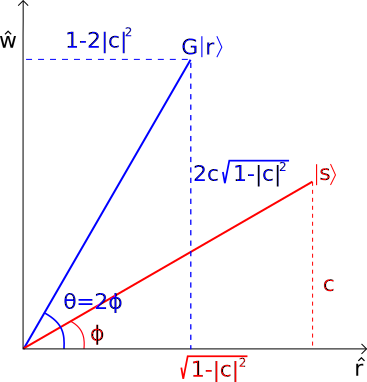
\includegraphics{./figures/trig}
	\end{center}
	\caption{\textbf{Grover search in the plane of the initial and target states.} To summarize Eqs.~(\ref{eq:sinq}), (\ref{eq:s0}), (\ref{eq:s1}), and \eqref{eq:theta_derv}, we depict the states $G\ket{r}$ and $\ket{s}$.   The answer state $\ket{w}$ is parallel to the ordinate axis.  The abscissa is the orthogonal state $\ket{r}$ defined in Eq.~\eqref{eq:r}.  The uniform superposition of all states is $\ket{s}$ and is characterized in Eqs.~\eqref{eq:s1} and \eqref{eq:s0}.  If $\phi_r$ is the angle between the $\hat{r}$ axis and $\ket{s}$ then the Grover operator $G$ performs a rotation of $2\phi_r$.  After $O(\sqrt{N})$ applications of the $G$ to the state $\ket{s}$, there is high probability that measurement will result in marked state $w$.  }
	\label{fig:trig}
\end{figure}


Thus, after $k$ iterations, the initial state with angle $\phi_r$ has been rotated to a vector characterized by angle $\Phi_k=k(2\phi_r)+\phi_r$.  When $\Phi_k$ is close to $\pi/2$, we have accomplished the goal of creating high overlap with the answer.  So, if $N$ is large, then the state $\ket{s}$ is approximately $\ket{r}$.  Then, we will need the following to be approximately satisfied.
\begin{eqnarray}
	\Phi_k=\frac{\pi}{2}&=&(2k+1)\phi_r\\
	\frac{\pi}{2\phi_r}&=& 2k+1\\
	k&=& \frac{\pi}{4\phi_r}-\frac{1}{2}
	\label{eq:iter_derv}
\end{eqnarray}
From Eqs.~\eqref{eq:s0} and \eqref{eq:s1} we have that $\sin\phi_r=1/\sqrt{N}$.  Using the small angle approximation, we say $\phi_r\approx 1/\sqrt{N}$.  Substituting into Eq.~\eqref{eq:iter_derv} we have
\begin{equation}
	k= \frac{\pi}{4}\sqrt{N}-\frac{1}{2}\approx \frac{\pi}{4}\sqrt{N}.
	\label{eq:scaling}
\end{equation}
Hence, the algorithm obtains the answer with high probability after a number of iterations that is scales as $\sqrt{N}$.


\subsection{Lower bound for Grover search}
Briefly, note that Grover search  is optimal with respect to the number of oracle calls it makes~\cite{Preskill98,Bennett97}.  Historically, its proof is important because of the technique that was used in the proof: the hybrid method. 

Grover algorithm, which relies on the oracle to find a marked item in time $O(\sqrt{N})$ can be proved optimal by changing a critical subset of oracle outputs such that the errors cannot be detected in time $\Omega(\sqrt{N})$~\cite{Bennett97}. This lower bound proof technique is a precursor to the widely used adversary method. 
The idea is an adversary makes modification of the true oracle on a subset of critical answers to trick you. Any quantum algorithms that access the oracle less than some lower bound is not sensitive to critical changes of the oracle.  For the Grover search problem, if the oracle is accessed less than $O(\sqrt{N})$ times, then for any algorithm (Grover or otherwise), there is an oracle for which the algorithm  will fail to distinguish the desired object from any other with high probability~\cite{Bennett97}. %This technique, along with the polynomial method~\cite{Beals98} and its many generalizations, are the two main techniques for proving lower bounds in the quantum query model.



% The classical analogue is boosting success probability of an event by repetition.
% To quote E. Farhi: `If you give me a probability, through repetition I can give you certainty.' 
%\alert{Incomplete\dots}  If $k$ independent trials each have a probability $p$ of success, then the probability to get the correct answer after $k$ repetitions is $1-(1-p)^k$. Defining a variable $s$ through $\exp(-1/s)=1-p$, the probability to err is decaying as $\exp(-k/s)$. The Chernoff bound says the probability of error decreases exponentially fast.  This holds when each trial is independent so after $1/p$ trials we expect event has occurred after $N$ trials is $N(1-p)$.   Then because each trial is independent the probability that each event is successful can be summed.  Thus after $1/p$ trials we expect with probability  event has occurred after $N$ trials is $N(1-p)$.   \alert{end(Incomplete)}

% Three extensions are worth mentioning.  First, amplitude amplification is a general framework for quantum algorithms such as Grover search and was first introduced in ref.~\cite{BHMT00}.  Second, there is a continuous version of Grover algorithm that was first discussed in~\cite{FG98} and is also discussed in\cite{NC01}.  Finally, we mention that quantum walks have lead to many extensions of Grover search.  A review can be found by Ambainis~\cite{Amb05}.

% Chapter 5: Complexity

\end{document}
